\documentclass[11pt]{book}
\usepackage[a4paper, margin=2.5cm]{geometry}

\usepackage[hidelinks]{hyperref}
\usepackage[french]{babel}
\usepackage{rotating}
\usepackage{wrapfig}
\usepackage{graphicx}
\usepackage{siunitx}
\usepackage{array}
\usepackage{enumerate}

% Theorems and definitions
\usepackage{amsthm}
\usepackage[framemethod=tikz]{mdframed}


% Math
\usepackage{amscd}
\usepackage{amsmath}
\usepackage{gensymb} % symbole degré: \degree
\usepackage{parskip}

\theoremstyle{definition}
\newmdtheoremenv[
  hidealllines=true,
  leftline=true,
  innerleftmargin=10pt,
  innerrightmargin=10pt,
  innertopmargin=1ex,
  innerbottommargin=1ex,
]{definition}{Définition}

\newcommand{\pbs}[1]{\let\temp=\\#1\let\\=\temp}
\newcommand{\tbf}[1]{\textbf{#1}}
\newcommand{\cov}{\ensuremath{\text{cov}}}

\begin{document}
\frontmatter
    \pagestyle{plain}

    \begin{titlepage}
    \thispagestyle{empty}
    \begin{center}
        \mbox{}\\[-29mm]
        \Large
        \rule[0.5ex]{\textwidth}{0.3mm}\\[1mm]
        Haute Ecole d'Ingénierie et de Gestion du Canton de Vaud\\[1mm]
        \rule[0.5ex]{\textwidth}{0.3mm}\\[2cm]
        \rule[0.5ex]{\textwidth}{0.5mm}\\
        \huge\textbf{Techniques de mesure \\
            et \\analyse de données\\
            \rule[0.5ex]{\textwidth}{0.5mm}}\\
        \vspace{1.5cm}
        \Large
        Département TIN - Technologies Industrielles\\[3mm]
        Profs. Cédric Bornand, Michel Demierre, Laurent Jolissaint\\[3mm]
        1er août 2019
    \end{center}
\end{titlepage}


    \tableofcontents

    \chapter*{Note}

Le matériel présenté dans ce document consiste en une reprise, avec beaucoup d'apports personnels et de modifications, des cours présentés par les Profs. Lorenzo Zago et Jacques Unger de la HEIG-VD. Nous tenons à les remercier de nous avoir transmis l'intégralité de leurs documents de cours et laboratoire.

Ces documents ont été eux-mêmes basés sur une compilation de plusieurs sources - polycopiés préexistants à la \href{http://www.heig-vd.ch}{HEIG-VD}, \href{http://wikipedia.org}{Wikipédia}, et contributions d'auteurs librement disponibles sur internet.


\mainmatter

    \chapter{Introduction}
\label{chap:introduction}

\section{Techniques de mesure, métrologie, analyse des données}

En ingénierie, et dans toutes les branches scientifiques, les informations sur les systèmes physiques, construits par l'humain, ou naturels, sont obtenues par des \textbf{mesures}. deux questions essentielles se posent alors à l'expérimentateur:
\begin{enumerate}
\item comment mesurer de la manière la plus juste possible,
\item et comment déduire, des mesures brutes, l'information recherchée ?
\end{enumerate}
La première partie est du domaine de ce que nous pouvons nommer les \textbf{techniques de mesures}, accompagnée des règles de la \textbf{métrologie}. La seconde partie constitue le vaste domaine de \textbf{l'analyse des données}. Dans ce cours, nous traiterons tout d'abord des techniques des mesures, logiquement suivies de la présentation des techniques d'analyse de données.

\section{Utilité de la métrologie}

Les techniques de mesure ont recours à la métrologie, terme qui se traduit, au sens étymologique, par \textless\textless\ science de la mesure\ \textgreater\textgreater. Avant d'entrer dans le vif du sujet, à savoir les techniques de mesure, il est donc nécessaire de bien comprendre quels sont les défis résolus par la métrologie.

La métrologie s'intéresse traditionnellement à la détermination de caractéristiques (appelées grandeurs) qui peuvent être fondamentales comme par exemple une longueur, une masse, un temps, ou dérivées de grandeurs fondamentales comme par exemple une surface, une vitesse (notons que dans beaucoup de domaines, comme celui des essais des matériaux, la médecine ... il existe des unités spécialisées qui n'ont pas de lien forcément direct avec les unités fondamentales ci-dessus, mais qui sont néanmoins parfaitement définies).

Quoi qu'il en soit, mesurer une grandeur physique consiste à lui attribuer une valeur quantitative en prenant pour référence une grandeur de même nature appelée unité. Dans le langage courant des métrologues, on entend souvent dire \textless\textless\ mesurer c'est comparer\ \textgreater\textgreater.

\begin{figure}[ht]
   \centering
   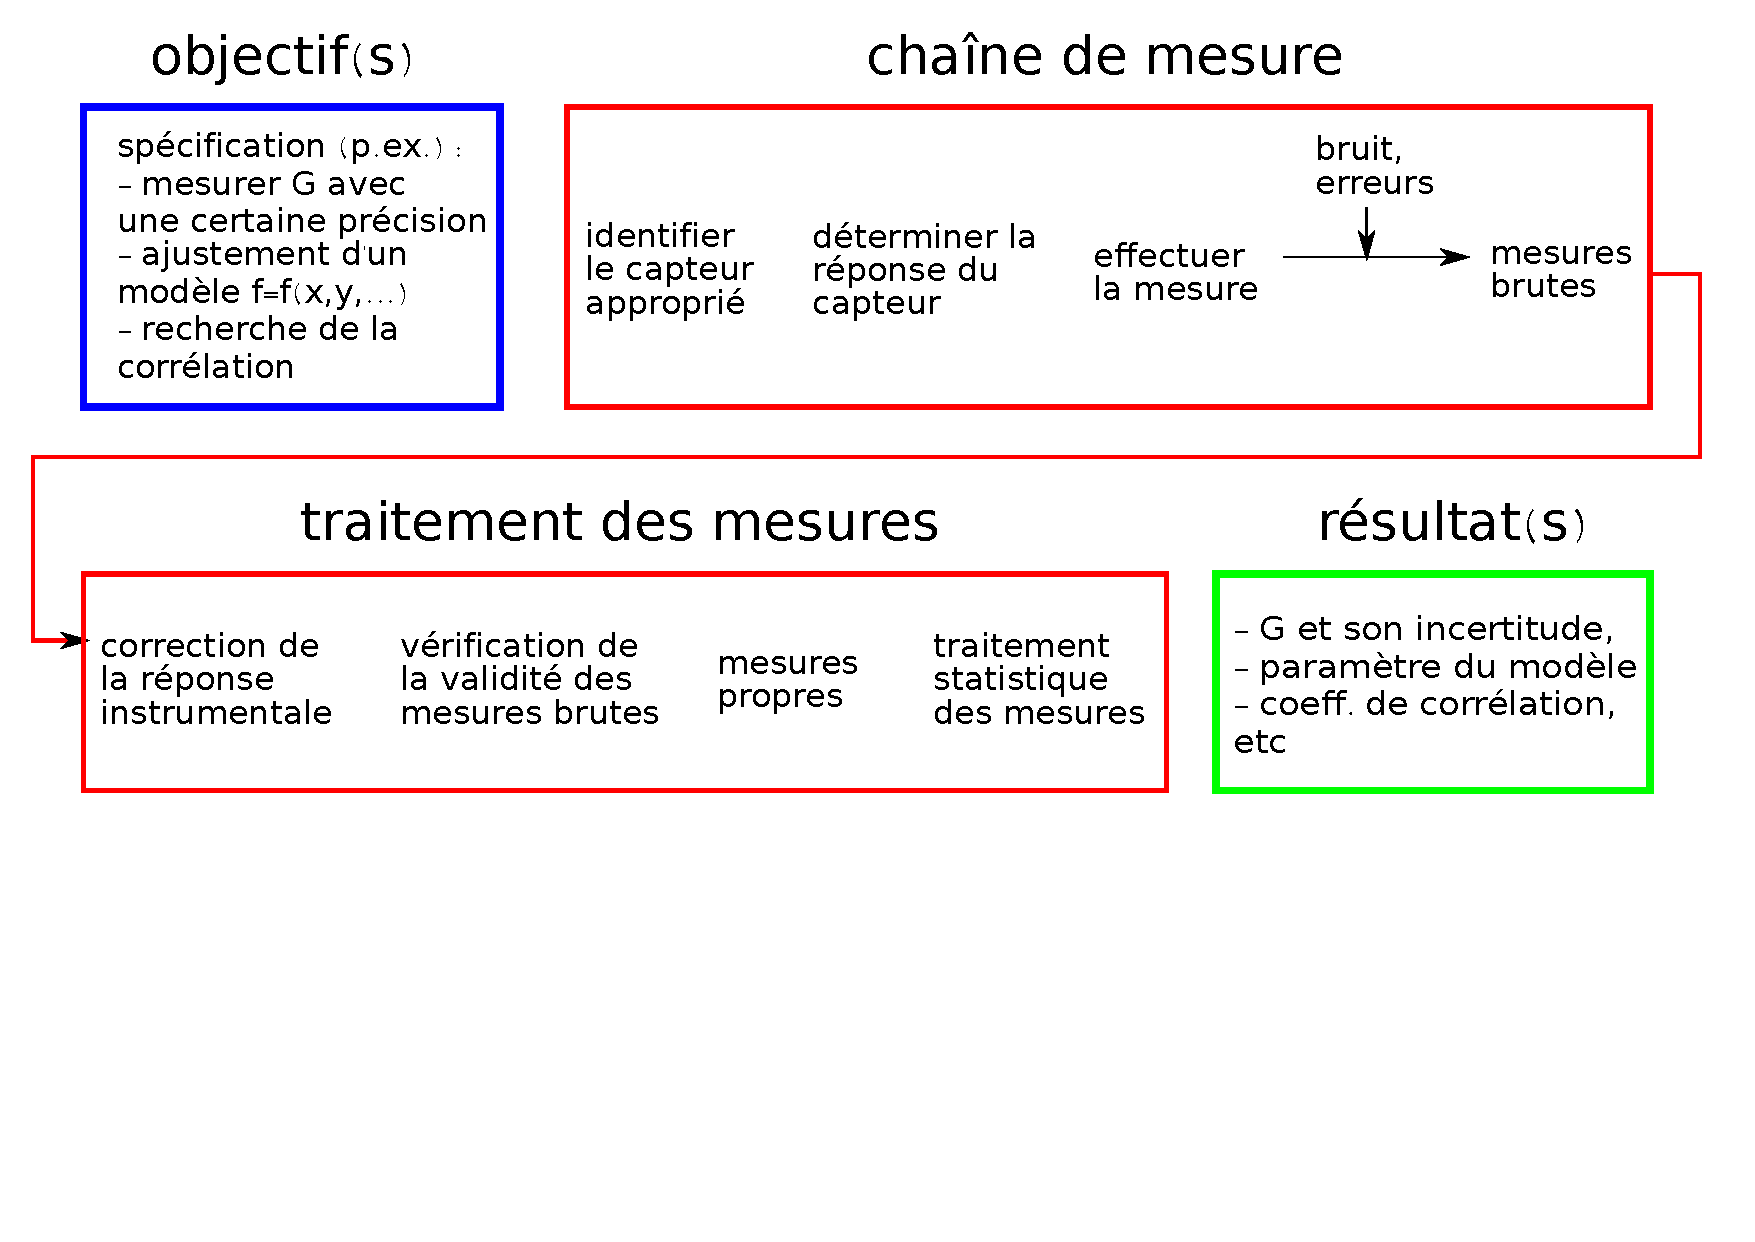
\includegraphics[width=0.9\textwidth]{assets/figures/flowChartTechMes.pdf}
   \caption{Techniques de mesure et traitement des données: les étapes clés.}
   \label{fig:flowchartTechMes}
\end{figure}
Les résultats des mesures servent à prendre des décisions dans de nombreux domaines, tels que:

\begin{itemize}
   \item validation d'une hypothèse scientifique,
   \item acceptation d'un produit (conformité à une exigence),
   \item réglage d'un paramètre dans le cadre du contrôle d'un procédé de fabrication,
   \item protection de l'environnement,
   \item définition des conditions de sécurité d'un produit ou d'un système.
\end{itemize}

L'ensemble de ces décisions concourt à la qualité des produits ou des services: on peut quantifier (ou caractériser) la qualité d'un résultat de mesure grâce à son incertitude.
En effet sans incertitude les résultats de mesure ne peuvent plus être comparés:

\begin{itemize}
   \item soit entre eux (essais croisés),
   \item soit par rapport à des valeurs de référence spécifiés dans une norme ou une spécification (conformité d'un produit).
\end{itemize}

Le diagramme de la figure  ~\ref{fig:flowchartTechMes} représente les différentes étapes nécessaires à la réalisation d'un système de mesure, depuis l'acquisition au traitement des mesures. C'est sur cette base que les chapitres ont été définis:

\begin{description}
   \item[Chapitre \ref{chap:introduction}] Introduction
   \item[Chapitre \ref{chap:si}] Le système international d'unités
   \item[Chapitre \ref{chap:measurement-chain}] La chaîne de mesure
   \item[Chapitre \ref{chap:measurement-chain-modelisation}] Modélisation de la chaîne de mesure
   \item[Chapitre \ref{chap:sensors}] Capteurs
\end{description}

La 2e partie traite de l'analyse des données:

\begin{description}
\item[Chapitre \ref{chap:measurements}] La mesure et sa représentation
\item[Chapitre \ref{chap:measurements-stochastic}] La mesure vue comme une variable aléatoire. Distributions usuelles des
variables aléatoires.
\item[Chapitre \ref{chap:measurements-multidimentional}] Mesures multidimensionnelles, corrélations, budget d'erreur
\item[Chapitre \ref{chap:model-adjustment}] Ajustement d'un modèle sur une série de mesures
\end{description}

\textbf{A la fin de ce cours, vous devriez être capable de concevoir un système de mesure d'une grandeur physique donnée, et de traiter les données enregistrées pour en tirer les informations désirées.}

    \chapter{Le système international d'unité (SI)}
\label{chap:si}

Le \textbf{Système international d'unités (abrégé SI)}, basé sur le \textbf{système métrique}, est le système d'unités le plus largement employé du monde. Il s'agit d'un système d'unités décimal (on passe d'une unité à ses multiples ou sous-multiples à l'aide de puissances de 10). C'est la Conférence générale des Poids et mesures (CGPM), rassemblant des délégués des états membres de la Convention du Mètre, qui décide de son évolution, tous les quatre ans, à Paris.

L'abréviation de \textless\textless\ Système international\ \textgreater\textgreater est SI, \textbf{quelle que soit la langue utilisée}\footnote{oui, \textit{même} en anglais}. La norme internationale ISO 1000 (ICS 01 060) décrit les unités SI et les recommandations pour l'emploi de leurs multiples et de certaines autres unités.

\section{Les sept unités de base SI}

\subsection{Origine}

Le nombre minimal d'unités possibles est basé sur le nombre minimal de grandeurs indépendantes et fondamentales permettant de décrire les lois de l'Univers. On comprendra aisément que l'\textbf{espace}, le \textbf{temps} et la \textbf{masse} sont des grandeurs ne pouvant pas s'exprimer les unes en fonction des autres, et que ces trois grandeurs définissent forcément \textbf{les trois premières unités fondamentales} de tout système métrologique, qui sont respectivement, en unités SI, le mètre, la seconde, le kilogramme.

Il existe une quatrième grandeur fondamentale, la \textbf{charge électrique}, irréductible aux  précédentes: on ne peut pas traduire la charge de l'électron ou du proton en une combinaison de masse, distance, et/ou temps~! A noter que c'est l'unité du courant électrique, soit la quantité de charge électrique qui passe dans un conducteur par unité de temps, qui constitue la quatrième unité fondamentale - l'ampère (A) - et non l'unité de la charge, le coulomb (C).

Pour continuer, il existe encore d'autres grandeurs fondamentales dont on ne parle presque jamais en dehors du monde de la physique subatomique: les charges liées aux interactions entre les particules fondamentales constitutives des protons et neutrons (les quarks), ainsi qu'entre les électrons et leur différentes versions (positron, muon etc.) Ces deux interactions se nomment l'interaction forte (pour les quarks) et faible (pour les électrons), mais ont une portée se limitant essentiellement aux dimensions du noyau de l'atome, et leurs effets ne se font ressentir que lors des expériences de physique des particules.

De la même manière que la charge électrique est le véhicule de la force électromagnétique, il existe des charges véhiculant les interactions forte et faible (nous ne les décrirons pas ici). Or, ces charges ne sont pas exprimables en termes des 4 unités fondamentales précédentes, elles constituent par conséquent de nouvelles grandeurs indépendantes, pour lesquelles des unités sont définies. Ceci dit, étant donné que ces charges n'ont d'importance que dans le domaine spécialisé de la physique des particules, et qu'elles sont loin d'avoir des applications courantes dans le monde actuel (hormis dans le domaine de l'imagerie médicale nucléaire), ces unités ne sont pas (encore) incluses comme unités fondamentales SI.

Aux quatre unités fondamentales ci-dessus, le système SI ajoute trois autres unités, le \textbf{kelvin} pour la température, la \textbf{candela} pour les mesures photométriques (quantité de lumière) et la \textbf{mole}, pour la quantité de matière.

Formellement, le kelvin et la candela ne sont pas des unités fondamentales: la température est en fait une mesure de l'énergie d'agitation thermique (oscillation, vitesse) des particules constituantes d'un corps à une température donnée; un flux de lumière n'est rien d'autre qu'un flux de photons véhiculant une certaine énergie. Or, l'énergie est exprimable en termes de distance, de masse et de temps.

La mole est en revanche une unité assez particulière, puisqu'elle ne correspond à aucune grandeur fondamentale des lois de la physique, au contraire des unités ci-dessus. Elle trouve son origine en chimie, où l'on a trouvé bien plus pratique, pour désigner un nombre d'atomes ou de molécules au sein d'une solution, de les regrouper par rapport à un nombre de bases, très grand, le nombre d'Avogadro, égal à $6.022141293\times 10^{23}$, typique du nombre d'atomes/molécules que l'on trouve dans les préparations de chimie\footnote{on consultera avec intérêt la page Wikipédia dédiée à ce sujet}. Il est en effet par exemple plus simple d'indiquer qu'il y a 3.5 moles d'une certaine molécule dans une solution donnée que de dire qu'il y en a $21.08\times 10^{23}$.

\subsection{Définitions}

Considérons l'unité de distance fondamentale, le mètre. Afin que cette référence soit disponible partout dans le monde, nous pourrions par exemple reproduire le mètre étalon conservé au \textbf{Bureau international des Poids et mesures (BIPM)} à Sèvres, France. Cette procédure présente cependant deux inconvénients majeurs : (1) tout procédé de reproduction ne saurait être exempt d'erreurs, (2) il faut avoir accès au mètre étalon.

Pour pallier à ces inconvénients, il a été décidé de définir le mètre non plus par rapport à un étalon physique, un objet bien réel, mais d'utiliser une propriété fondamentale de la matière, indépendante du temps et de l'espace, c'est-à-dire disponible partout et tout le temps, et parfaitement invariable, ou constante. On a donc choisi de définir le mètre comme la distance parcourue par la lumière, dans le vide, durant $1/299'792'458$ secondes exactement. Tout laboratoire bien équipé pourra reproduire cette expérience, et donc définir avec toute la précision requise une distance, entre deux plans de référence bien accessibles, égale au mètre ou à un de ses multiples ou sous-multiples.

L'exemple du mètre décrit le principe que l'on applique aujourd'hui à la définition des unités fondamentales SI. Seul le kilogramme est encore défini par rapport à un objet matériel concret – une masse composée d'un alliage de platine et d'iridium conservé au BIPM - susceptible de s'altérer. Des recherches ont d'ailleurs actuellement lieu pour remplacer cette définition par une autre, utilisant cette fois un phénomène physique, inaltérable par nature.

\newpage

\begin{center}
\begin{tabular}[t]{>{\pbs\raggedright}p{2.5cm}
                   >{\pbs\centering}p{2.2cm}
                   >{\pbs\centering}p{2.3cm}
                   >{\pbs\raggedright}p{7cm}}
\hline\hline
\textbf{Grandeur} & \textbf{Nom} & \textbf{Symbole SI} & \textbf{Définition, remarques}\\
\hline
longueur & mètre & m &
Le mètre est la longueur du trajet parcouru dans le vide par la lumière pendant 1/299'792'458 secondes. Historiquement, la première définition officielle du mètre (1791) était basée sur la circonférence de la terre, et valait 1/40'000'000 du périmètre de notre planète.
\\ \hline
masse & kilogramme & kg &
Le kilogramme est la masse d'un cylindre composé d'un alliage de platine (90 \%) et d'iridium (10\%), conservé au Bureau international des Poids et mesures. Historiquement, la définition du kilogramme était la masse d'un décimètre cube d'eau.
\\ \hline
temps & seconde & s &
La seconde est la durée de temps associée à 9'192'631'770 oscillations de l'onde électromagnétique (photons) émise lors de la transition des électrons entre les deux sous-niveaux d'énergie de l'état d'énergie fondamental de l'atome de césium 133 ($^{133}$Cs) à la température de 0 kelvin. La seconde était à l'origine basée sur la durée (instable) du jour terrestre, d'une durée de 86'400 secondes.
\\ \hline
\end{tabular}
\end{center}
\begin{center}
\begin{tabular}[t]{>{\pbs\raggedright}p{2.5cm}
                    >{\pbs\centering}p{2.2cm}
                    >{\pbs\centering}p{2.3cm}
                    >{\pbs\raggedright}p{7cm}}
\hline
courant électrique & ampère & A &
L'ampère est l'intensité d'un courant constant qui, maintenu dans deux conducteurs parallèles, rectilignes, de longueur infinie, de section circulaire négligeable et placés à une distance de un mètre l'un de l'autre dans le vide produirait entre ces conducteurs une force égale à $2\times10^{-7}$ newton par mètre de longueur.
\\ \hline
température & kelvin & K	&
Le kelvin, unité de température thermodynamique, est la fraction 1/273.16 de la température thermodynamique du point triple de l'eau. Le point triple de l'eau est, dans le diagramme pression-température, un point où l'eau peut exister dans les trois états, soit solide, liquide et gazeux. La température associée à cet état est de 273.16 K. A noter que l'on écrit K et non $^{\circ}$K.
\\ \hline
quantité de matière & mole & mol	&
La mole est la quantité de matière d'un système contenant autant d'entités élémentaires qu'il y a d'atomes dans 0.012 kg de carbone 12 ($^{12}$C). Ce nombre d'entités élémentaires est appelé nombre d'Avogadro, et vaut $\mathcal{N}_{A}=6.02214129(27)\times10^{23}\,\text{mol}^{-1}$. Lorsque l'on emploie la mole, les entités élémentaires doivent être spécifiées et peuvent être des atomes, des molécules, des ions, des électrons, d'autres particules ou des groupements spécifiés de telles particules.
\\ \hline
\end{tabular}
\end{center}
\begin{center}
\begin{tabular}[t]{>{\pbs\raggedright}p{2.5cm}
                    >{\pbs\centering}p{2.2cm}
                    >{\pbs\centering}p{2.3cm}
                    >{\pbs\raggedright}p{7cm}}
\hline
intensité lumineuse & candela & cd &
La candela est l'intensité lumineuse, dans une direction donnée, d'une source qui émet un rayonnement monochromatique de fréquence $540\times10^{12}$ hertz et dont l'intensité énergétique dans cette direction est de 1/683 watt par stéradian.
\\ \hline\hline
\end{tabular}
\end{center}


\section{Unités dérivées}


Les unités dérivées font partie du système SI et sont déduites des sept unités de base.
\begin{center}
\begin{tabular}[t]{>{\pbs\raggedright}p{28mm}
                    >{\pbs\centering}p{15mm}
                    >{\pbs\centering}p{12mm}
                    >{\pbs\centering}p{22mm}
                    >{\pbs\centering}p{22mm}
                    >{\pbs\raggedright}p{32mm}}
\hline\hline
\textbf{Grandeur} & \textbf{Nom} & \textbf{Sym. SI} & \textbf{lien avec autres unités} & \textbf{lien avec unités de base} & \textbf{Relation physique}\\
\hline
Fréquence & hertz & Hz & --- & 1/s & Fréquence = 1/période \\ \hline
Force & newton & N & --- & kg m/s$^2$ & Force = masse $\times$ accélération \\ \hline
Contrainte, pression & pascal & Pa	& N/m$^2$ & kg/m/s$^2$ & Pression = force / surface \\ \hline
Energie, travail, quantité de chaleur & joule & J & N m & kg m$^2$/s$^2$	& Travail = force$\times$distance;
énergie cinétique = masse$\times$vitesse$^2$/2 \\ \hline
Puissance, flux énergétique et flux thermique & watt & W & J/s & kg m$^2$/s$^3$ & Puissance = travail / temps \\ \hline
Charge électrique, quantité d'électricité & coulomb & C & --- & A s & Charge = courant$\times$temps \\ \hline
\end{tabular}
\end{center}

\begin{center}
\begin{tabular}[t]{>{\pbs\raggedright}p{28mm}
                    >{\pbs\centering}p{17mm}
                    >{\pbs\centering}p{11mm}
                    >{\pbs\centering}p{22mm}
                    >{\pbs\centering}p{22mm}
                    >{\pbs\raggedright}p{32mm}}
\hline
Force électromotrice, différence de potentiel (tension) & volt & V & J/C & kg m$^2$/s$^3$/A & Tension = travail / charge
\\ \hline
Résistance électrique & ohm & $\Omega$ & V/A & kg m$^2$/s$^3$/A$^2$ & Résistance =  tension / courant
\\ \hline
Conductance électrique & siemens & S	& A/V & s$^3$A$^2$/kg/m$^2$ & Conductance = courant / tension
\\ \hline
Capacité électrique & farad & F & C/V & s$^4$A$^2$/kg/m$^2$ & Capacité = charge / tension
\\ \hline
Induction magnétique & tesla & T	& V s/m$^2$ & kg/s$^2$/A & Induction = tension$\times$temps / surface
\\ \hline
Flux d'induction magnétique & weber & Wb	& V s & kg m$^2$/s$^2$/A & Flux d'induction = tension$\times$temps
\\ \hline
Inductance électrique & henry & H & V s/A & kg m$^2$/s$^2$/A$^2$ & Inductance = tension$\times$temps / courant
\\ \hline
Température & degré Celsius & $^{\circ}$C & --- & K & T [$^{\circ}$C]=T [K]-273.15
\\ \hline
Flux lumineux & lumen & lm & --- & cd sr & ---
\\ \hline
Éclairement lumineux & lux & lx & --- & cd sr/m$^2$ & ---
\\ \hline
Nombre de désintégrations par seconde (radioactivité) & becquerel & Bq & --- & 1/s & ---
\\ \hline
Dose de radioactivité absorbée & gray & Gy & J/kg & m$^2$/s$^2$ & ---
\\ \hline
Équivalent de dose radioactivité absorbée & sievert & Sv & J/kg & m$^2$/s$^2$ & ---
\\ \hline
Activité catalytique & katal & kat & --- & mol/s & ---
\\ \hline\hline
\end{tabular}
\end{center}


\section{Préfixes du système SI}


Les préfixes du système international d'unités simplifient la manipulation des mesures qui ont des rapports élevés d'unité (par exemple de 0.1 cm à 1'000 m). Ces préfixes renvoient à des multiples et des fractions de 10 ou de 1000.  Les préfixes et noms correspondants sont donnés dans le tableau ci-après. On notera que les préfixes s'écrivent avec une lettre minuscule à partir et en dessous de l'échelle des milliers. \textbf{Il est fondamental d'observer très exactement ces conventions internationales}.

\begin{table}[htbp]
%\footnotesize
\begin{center}
\begin{tabular}{>{\pbs\raggedright}p{1cm}>{\pbs\raggedright}p{1.4cm}>{\pbs\centering}p{1.5cm}ll}
$10^n$ & Préfixe & Sym. SI & Nombre décimal & Échelle \\ \hline
$10^{24}$  & yotta &     Y & 1'000'000'000'000'000'000'000'000 & Quadrillion \\
$10^{21}$  & zetta &     Z & 1'000'000'000'000'000'000'000 & Trilliard \\
$10^{18}$  &   exa &     E & 1'000'000'000'000'000'000 & Trillion \\
$10^{15}$  &  péta &     P & 1'000'000'000'000'000 & Billiard \\
$10^{12}$  &  téra &     T & 1'000'000'000'000 & Billion \\
$10^{9}$   &  giga &     G & 1'000'000'000 & Milliard \\
$10^{6}$   &  méga &     M & 1'000'000 & Million \\
$10^{3}$   &  kilo &     k & 1'000 & Millier \\
$10^{2}$   & hecto &     h & 100 & Cent \\
$10^{1}$   &  déca &    da & 10 & Dix \\
$10^{0}$   &   --  &    -- & 1 & Unité \\
$10^{-1}$  &  déci &     d & 0.1	& Dixième \\
$10^{-2}$  & centi &     c & 0.01 & Centième \\
$10^{-3}$  & milli &     m & 0.001 & Millième \\
$10^{-6}$  & micro & $\mu$ & 0.000'001 & Millionième \\
$10^{-9}$  &  nano &     n & 0.000'000'001 & Milliardième \\
$10^{-12	}$ &  pico &     p & 0.000'000'000'001 & Billionième \\
$10^{-15	}$ & femto &     f & 0.000'000'000'000'001 & Billiardième \\
$10^{-18	}$ &  atto &     a & 0.000'000'000'000'000'001 & Trillionième \\
$10^{-21	}$ & zepto &     z & 0.000'000'000'000'000'000'001 & Trilliardième \\
$10^{-24	}$ & yocto &     y & 0.000'000'000'000'000'000'000'001 & Quadrillionième \\ \hline
\end{tabular}
\end{center}
\end{table}

\newpage

\section{Unités angulaires}

\begin{wrapfigure}[20]{l}[0pt]{5cm}
   \centering
   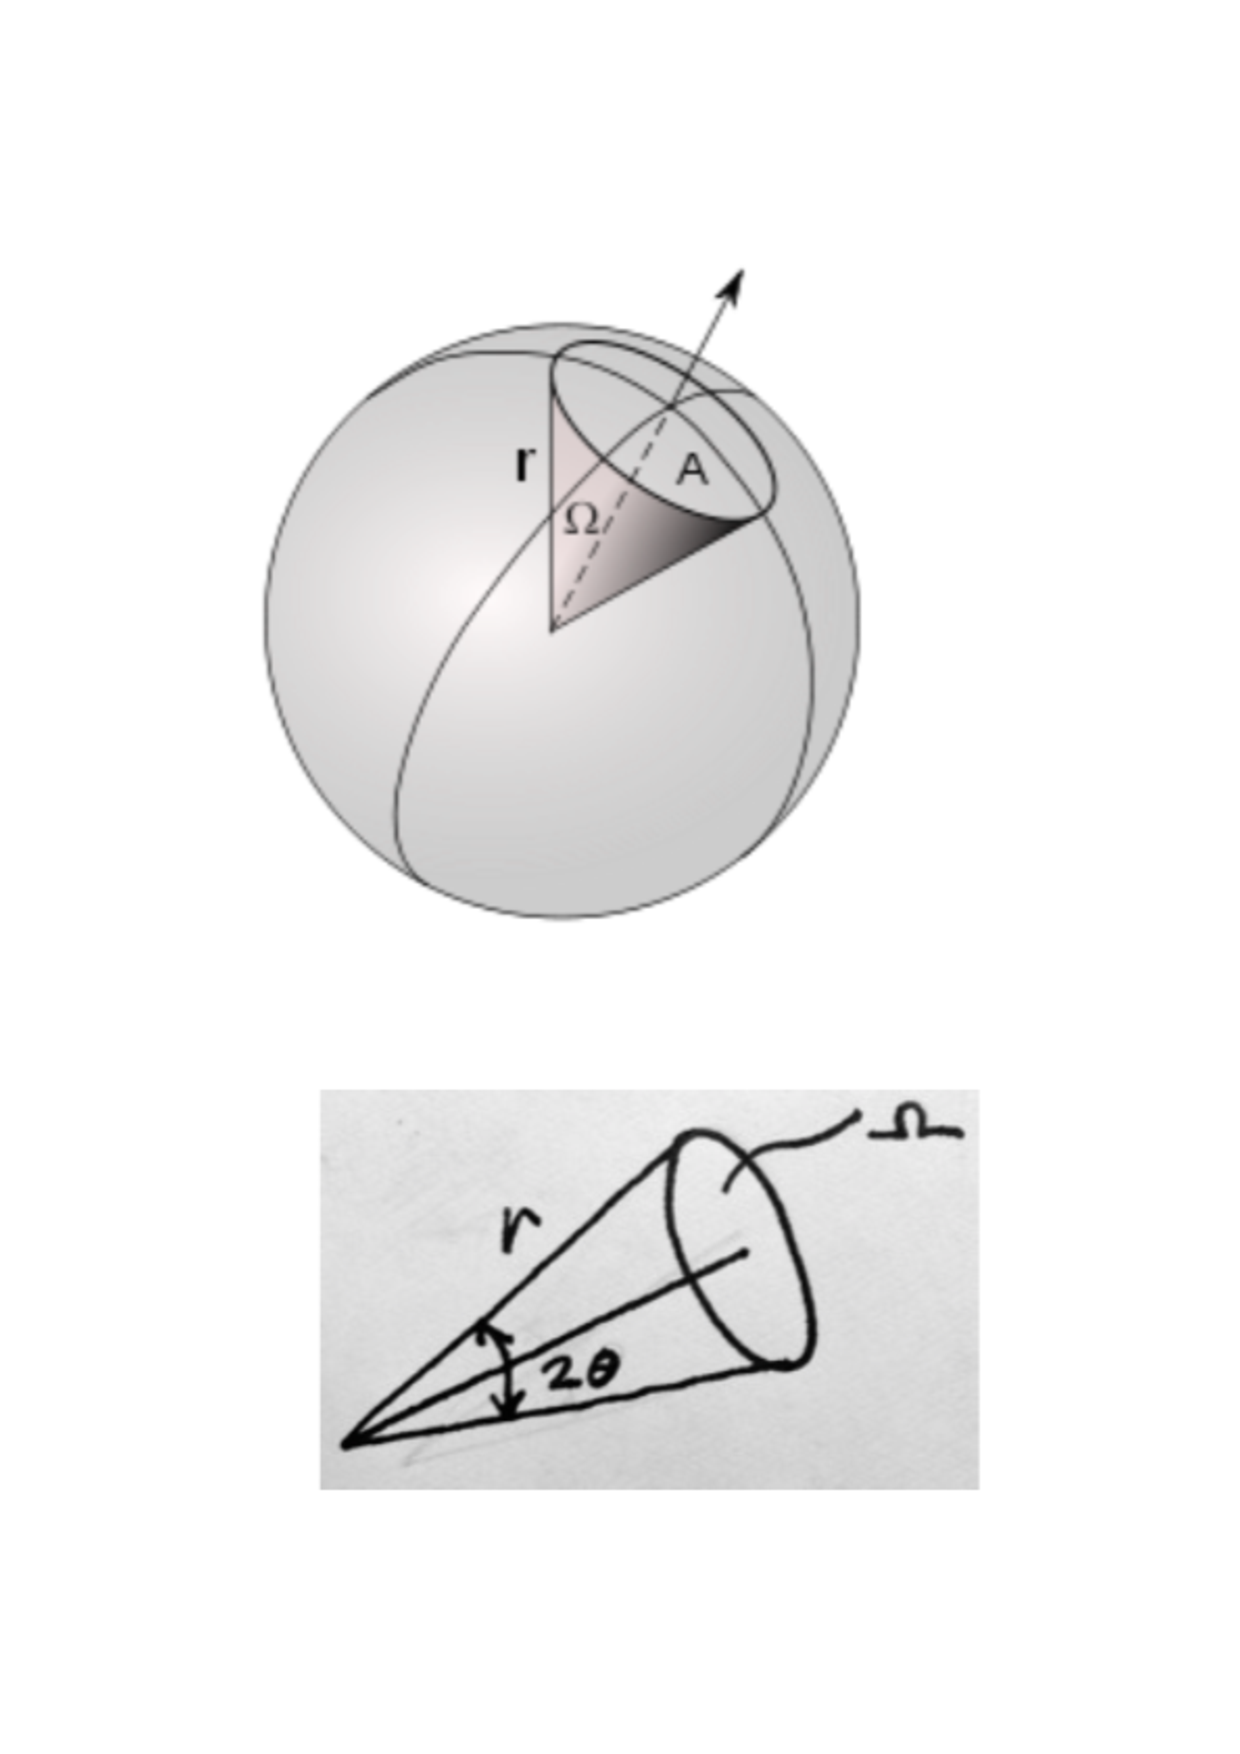
\includegraphics[width=5cm]{assets/figures/defAngleSolide.pdf}
   \caption{Définition de l'angle solide.}
   \label{fig:angles}
\end{wrapfigure}
À côté des unités de base et des unités dérivées, il existe deux unités angulaires:

\paragraph{L'unité d'angle plan: le radian (symbole: rad)} Soit un secteur de cercle de rayon $r$ et de longueur d'arc $l$. L'angle $\theta$ associé au secteur, en radian, est défini par le rapport
$$
\theta=\frac{l}{r}\ \ [\text{rad}]
$$
180$^\circ$ correspondant à $\pi$ rad, on a que 1 rad $\approx$ 57.3$^\circ$.

\paragraph{L'unité d'angle solide: le stéradian (symbole: sr)} Soit un cône dont l'angle au sommet est de $2\theta$ [rad], et soit $A$ l'aire de la calotte sphérique formée par l'intersection du cône avec la surface de la sphère de rayon $r$ (figure~\ref{fig:angles}). L'angle solide $\Omega$ associé au cône est défini par le rapport
$$
\Omega=\frac{A}{r^2}\ \ [\text{sr}]
$$
L'aire d'une sphère de rayon $r$ étant donnée par $4\pi\,r^2$, on trouve que l'angle solide de la sphère est égal à $4\pi$ sr, et de la demi-sphère $2\pi$. On peut aussi montrer que
$$
\Omega=2\pi(1-\cos\theta)
$$

Les grandeurs \textless\textless\ angle plan \ \textgreater\textgreater et \textless\textless\ angle solide \ \textgreater\textgreater sont des unités sans dimension - puisqu'il s'agit de rapport de longueurs et de surface - qui peuvent être indiquées ou non dans les expressions des unités dérivées.

\section{Règles d'écriture des unités et symboles SI}

\begin{itemize}

\item le nom de l'unité est un nom commun même pour les unités provenant de noms propres : volt, ampère, kelvin, tesla etc;
\item les symboles SI des unités sont écrits en police droite, et en minuscules, \textbf{sauf} si le nom de l'unité est dérivée d'un nom propre: dans ce cas la première lettre du symbole est en majuscule, par exemple N (Newton), J (Joule), V (Volta), Bq (Bequerel);
\item les symboles SI sont invariables au pluriel;
\item les symboles SI sont écrits sans point final;
\item les symboles SI doivent être placés après les valeurs numériques, en laissant un espace entre valeur et symbole, donc 30 m est juste, 30m ne l'est pas;
\item le produit de 2 unités est indiqué par un point, qui peut être omis si aucune confusion n'est possible, par exemple 1 mN est un millinewton et non un mètre-newton (c.-à-d. un joule), sinon nous aurions écrit m$\cdot$N !
\item le quotient est indiqué par une barre oblique, ou alors on peut utiliser les puissances négatives, comme avec m/s$^2$ ou m$\cdot$s$^{-2}$, mais pas ms$^{-2}$ car alors ms peut être interprété comme indiquant des millisecondes;
\item lorsque l'unité suit une valeur numérique, on ne met \textbf{jamais} de crochets autour de l'unité; on ne place l'unité entre crochets que dans les formules, par exemple la fameuse formule d'Einstein s'écrira
$$
E=mc^2\ \text{[J]}\ \ \ \ \text{mais par contre}\ \ \ \ E=10^6\ \text{J}
$$
\end{itemize}
Quelques exemples d'écriture  fausses et justes:

\begin{center}
\begin{tabular}{lll}
faux & juste & interprétation\\\hline
$99Kg$& 99 kg & 99 kilogramme\\
$25 [ms]$ & 25 ms & 25 milliseconde\\
$12 \mu v$ & 12 $\mu$V & 12 microvolt\\
100 K*m & 100 K$\cdot$m & 100 kelvin$\cdot$mètre\\\hline
\end{tabular}
\end{center}
    \input{src/15-chaîne-de-mesure}
    \chapter{Modélisation de la chaîne}
\label{chap:measurement-chain-modelisation}

Reprenant le schéma bloc des étapes clé des techniques de mesure de la figure \ref{fig:flowChartTechMes_chaine_de_mesure}, nous souhaiterions aborder le traitement des mesures. Toutefois nos connaissances de la chaîne de mesure sont encore insuffisantes: nous devons maintenant comprendre comment modéliser la chaîne de mesure afin d'avoir les outils et informations nécessaires aux traitements mathématiques qui vont suivre.

Pour résoudre le problème de la mesure, à savoir retrouver la valeur du mesurande à partir de la sortie du capteur, il faut inverser la fonction mathématique $F(X)$ liant le mesurande à la sortie. La difficulté vient du fait que F(X) est mal définie: du bruit s'ajoute au signal de sortie, les grandeurs d'influence modifient la fonction, les tolérances de fabrication conduisent à une fonction réelle légèrement différente de la fonction nominale. De plus les lois physiques qui régissent le capteur et la chaîne de mesure peuvent conduire à une expression mathématique complexe de la fonction.

\section{Approximations mathématiques}

Nous avons vu au chapitre \ref{chap:introduction} que les approximations mathématiques pouvaient être faites au travers de modèles de formes mathématiques diverses: linéaire, polynomiale ou découlant directement de la loi physique exploitée dans le capteur. Pour la suite de l'analyse, \textbf{nous ne considérerons ici que le cas linéaire.}

\section{Incertitudes}

Le modèle linéaire est une droite, ne passant pas nécessairement par l'origine, approchant au mieux la caractéristique de la chaîne de mesure:

\begin{center}
    \fbox{\textbf{Y = G X  + Of}}
\end{center}

Cette équation fait intervenir les deux paramètres G et Of, caractéristiques de la chaîne.

\begin{definition}
    Le gain $G$ est la pente de la caractéristique entrée-sortie.
\end{definition}

\begin{definition}
    Le décalage $Of$ est l'ordonnée à l'origine du modèle linéaire (de l'anglais \emph{offset}).
\end{definition}

Il est fondamental de ne jamais oublier qu'il ne s'agit là que d'une approximation de la courbe de réponse (forme de la réponse pas tout à fait droite, tolérances de fabrication), et de plus que cette approximation est variable dans le temps, en raison des grandeurs d'influence (vieillissement, température, ...) ou des conditions d'utilisation (effet de charge, perturbations,...). Le fabricant nous indique les valeurs nominales du gain et du décalage $G_{nom}$ et $Of_{nom}$.
On résout le problème de mesure sur la base de ces valeurs nominales, et l'on obtient alors une estimation $X_{m}$ de la grandeur d'entrée $X$:

\begin{center}
    \fbox{
        \begin{minipage}{0.96\textwidth}
            \textbf{\textit{Déf}. Erreur absolue (e) :}
            Écart entre la valeur mesurée et la vraie valeur 	$e = X_{m} - X$
            \newline
            \newline
            \textbf{\textit{Déf}. Erreur relative ($\epsilon$) : }
            \text{Quotient entre erreur absolue et vraie valeur  }	$\epsilon = \frac{e}{X}  \cong \frac{e}{X_{m}}$
        \end{minipage}
    }
\end{center}

Pour analyser l'erreur, il faut tenir compte des écarts entre la courbe réelle et son approximation linéaire dans les conditions de mesure, ainsi que du fait que cette approximation diffère légèrement de la droite nominale. Nous écrivons donc une nouvelle expression de la sortie Y
\begin{equation}
    Y = G_{reel}X + Of_{reel} + L(X,t)
\end{equation}
où $G_{reel}$ et $Of_{reel}$ représentent le modèle linéaire actuel, tenant compte des grandeurs d'influence et effets de charge. $L(X,t)$ représente l'écart entre la courbe et la droite du modèle actuel, ainsi que le bruit ajouté à la sortie. On ne connaît jamais ces trois termes, mais un étalonnage dans des conditions données des grandeurs d'influence permet au fabricant de spécifier les écarts maximum. Exprimons l'erreur:
\begin{gather}
    e = X_m - X =  Y - \frac{Of_{nom}}{G_{nom}} - X = \frac{G_{reel}X + Of_{reel} + L -Of_{nom}}{G_{nom}} - X\\
    e = X \cdot(\frac{G_{reel}}{G_{nom}}   - 1) +  \frac{Of_{reel} - Of_{nom}}{G_{nom}}   +  \frac{L}{G_{nom}}
\end{gather}
c.-à-d.
\begin{equation}
    e = X \cdot \alpha  + D + NL
\end{equation}
On constate alors que l'erreur est la somme de trois termes. Les deux premiers expriment des erreurs systématiques fonctions des grandeurs d'influence (dérive du modèle linéaire par rapport aux valeurs nominales), le troisième peut être assimilé à une erreur aléatoire.
\begin{center}
    \fbox{
        \begin{minipage}{0.95\textwidth}
            \textbf{\textit{Déf}. Erreur de gain  ($\alpha$) :}\\
            Erreur relative du gain de la chaîne: Gréel - GnomGnom  .  Correspond à une rotation de la courbe autour de l'origine. Provoque une erreur systématique proportionnelle au mesurande (calculable seulement si l'on connaît toutes les grandeurs d'influence)\\
            \\
            \textbf{\textit{Déf}. Erreur de décalage (D) :}\\
            Erreur absolue à l'origine: Ofréel - OfnomGnom  . Correspond à une translation verticale de la courbe de réponse. Provoque une erreur systématique constante, indépendante de X (calculable seulement si l'on connaît toutes les grandeurs d'influence)\\
            \\
            \textbf{\textit{Déf}. Erreur de non-linéarité (NL)}\\
            Écart entre la droite du modèle actuel et la courbe réelle de réponse. Fonction du mesurande, si bien qu'on la considère comme une grandeur aléatoire.
        \end{minipage}
    }
\end{center}
Le fabricant indique l'incertitude de la chaîne ou d'un appareil en combinant ces trois erreurs et le bruit interne.

\begin{center}
    \fbox{
        \begin{minipage}{0.96\textwidth}
            \textbf{\textit{Déf}. Incertitude de mesure :	}
            Valeur limite que peut prendre l'erreur (en valeur absolue), avec un certain degré de confiance, en général 99 \%. En d'autres termes, si l'on a spécifié une incertitude I, la valeur absolue de l'erreur e sera dans 99 \% des cas inférieure à I : 	|e| < I 	(99 fois sur 100)
        \end{minipage}
    }
\end{center}

\begin{figure}
    \centering
    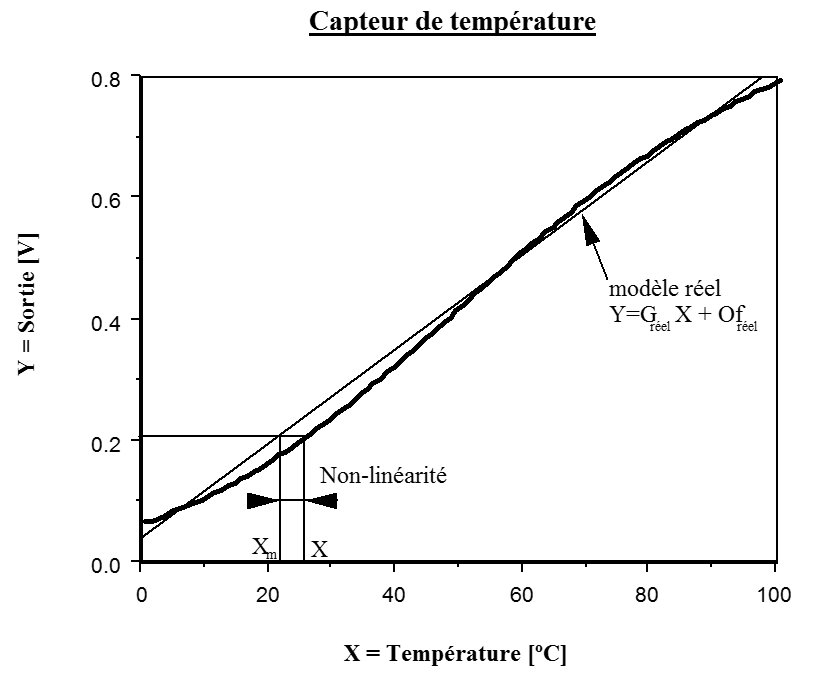
\includegraphics[height=8cm]{assets/figures/3_1_Non_Linearite.PNG}
    \caption{Non-linéarité.}
    \label{fig:Non-linéarité}
\end{figure}
La spécification de l'incertitude comprend deux termes, pour tenir compte du fait que l'une des composantes est proportionnelle à X. L'erreur de gain est toujours spécifiée sous forme d'une valeur relative $\alpha$ (en \%, \textperthousand ~ ou ppm, soit des facteurs de $10^{-2}, 10^{-3}, ou 10^{-6}$), alors que l'effet global du décalage, des non-linéarités et du bruit interne est spécifié comme un terme indépendant de X, soit sous forme absolue B (unités de X, ou unités d'affichage: divisions sur un écran analogique, digit sur un affichage numérique), soit sous forme relative $\beta$ par rapport à une grandeur caractéristique de la chaîne: gamme de mesure, étendue de mesure, ou pleine échelle.
\begin{equation}
    I = \alpha \cdot \text{lect} + B \cdot digit = \alpha \cdot \text{lect} + \beta \cdot \text{gamme}
\end{equation}

\begin{figure}[h]
    \centering
    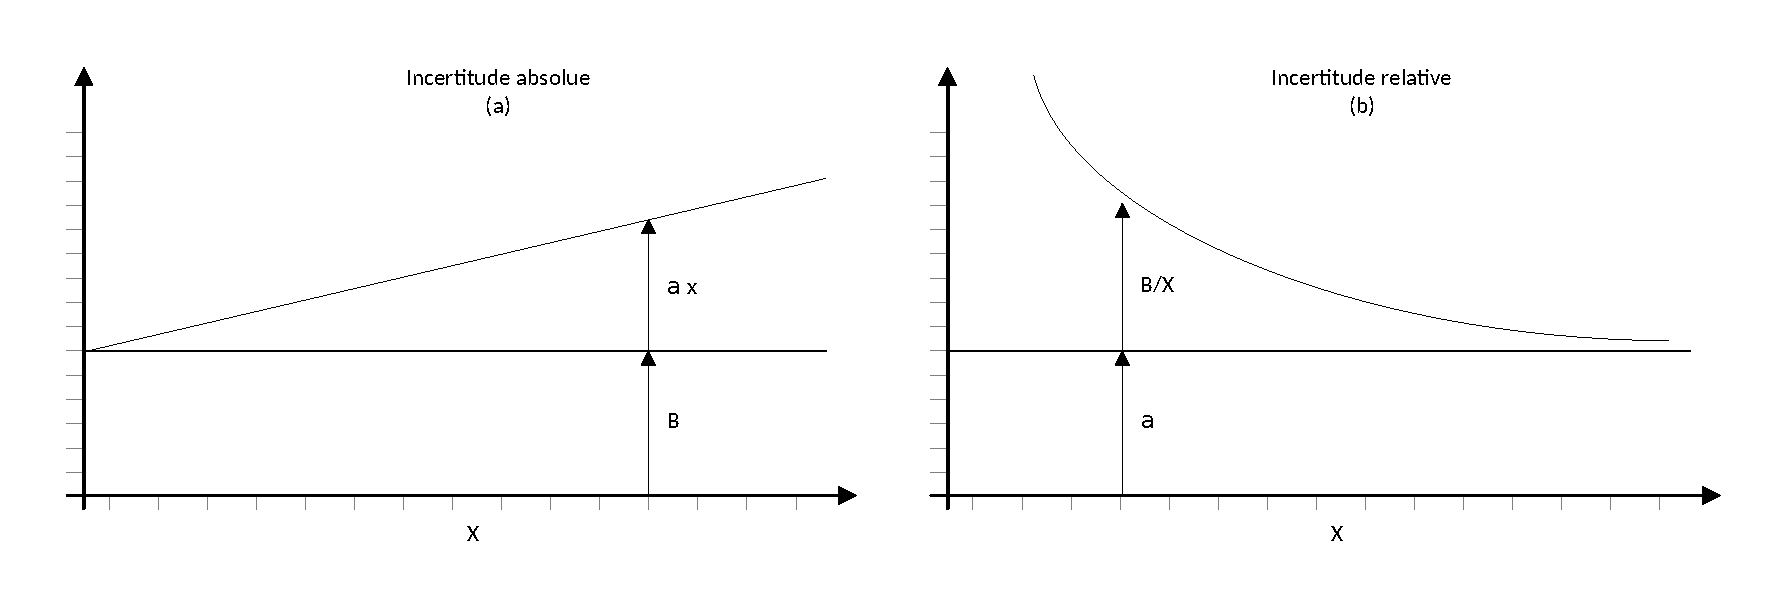
\includegraphics[height=10.7cm]{assets/figures/incertitudes.pdf}
    \caption{Évolution des incertitudes absolues et relatives en fonction du mesurande.}
    \label{fig:incertitudes_absolues_et_relatives}
\end{figure}

La figure \ref{fig:incertitudes_absolues_et_relatives} nous montre que l'incertitude absolue est maximum en haut de gamme, alors que l'incertitude relative tend vers l'infini lorsque X tend vers zéro. Lorsqu'on doit évaluer l'imprécision d'un système de mesure, on le fera soit en estimant l'incertitude absolue en haut de gamme, soit l'incertitude relative en bas de gamme (recherche du pire des cas).

Lorsqu'on fait l'évaluation d'un mesurande qui évolue dans une plage de variation donnée, on cherchera avantageusement à relativiser l'incertitude par rapport à la pleine échelle (PE, en anglais FS pour "Full Scale") de cette variation, et de l'exprimer alors en \%(PE) ou \%(FS). Par exemple, l'information fournie par un capteur de pression qui évolue entre 950 et 1100 mbar permet bien de savoir à quel endroit se trouve la pression le long des 150mbar d'évolution possible. Dans ce cas c'est donc bien la pleine échelle qui nous intéressera comme référence.

Par ailleurs, lorsqu'on cherche à faire une mesure d'une grandeur avec un appareil donné, on remarquera souvent que la valeur B augmente quasi proportionnellement avec la gamme alors que $\alpha$ reste assez stable quelle que soit la gamme. Ainsi, pour de bonnes mesures il est indispensable de choisir la plus petite gamme de mesure possible. On aura ainsi un B minimal.

\section{Calibrage et étalonnage}

Sur de nombreuses chaînes de mesure on dispose d'un amplificateur avec lequel on peut ajuster le gain et le décalage. On est alors amené, au moment de la mise en service de la chaîne, à ajuster cet amplificateur, de manière à obtenir la réponse la plus proche que possible de l'idéal (modèle nominal). C'est ce qu'on appelle le calibrage (en anglais: gauging ou calibration), opération qui vise à annuler les erreurs de gain et de décalage. Une autre opération consiste, sans modifier la chaîne, à déterminer son modèle réel, et l'écart entre le modèle réel et le modèle nominal. C'est l'opération d'étalonnage(en anglais: calibration). Cette opération peut être faite dans un but de correction ou de vérification. Dans ce dernier cas, la chaîne est acceptée si elle se trouve dans les tolérances, ou rejetée sinon. Dans le cas de la correction, alors un moteur de correction sera mis en oeuvre par l'utilisateur de la chaîne de mesure pour exploiter non pas le modèle nominal, mais le modèle réel mesuré.
On notera que la terminologie française est cette fois plus précise que la terminologie anglaise où la distinction entre calibrage et étalonnage ne se fait pas. Ce flou se retrouve en français lorsqu'on utilise l'anglicisme "calibration", alors que ce terme s'applique normalement à des méthodes de datation en dendrochronologie.
\begin{center}
    \fbox{
        \begin{minipage}{0.96\textwidth}
            \textbf{\textit{Déf}. Étalonnage :	}
            Ensemble des opérations permettant de déterminer le modèle réel de la chaîne de mesure, et donc de déterminer les erreurs de mesure par rapport au modèle nominal.\\

            \textbf{\textit{Déf}. Calibrage :	}
            Ensemble des opérations d'ajustage des différents réglages de la chaîne, pour l'amener à un fonctionnement aussi juste que possible, c'est-à-dire aussi proche que possible du modèle nominal.
        \end{minipage}
    }
\end{center}

Dans ces opérations, il faut imposer à l'entrée de la chaîne une valeur connue du mesurande, et observer la sortie de la chaîne. Quatre situations peuvent se présenter :
\begin{enumerate}[a)]
    \item Dans de très rares cas, on dispose d'un moyen d'imposer une valeur exacte (par exemple une tension nulle au moyen d'un court-circuit).
    \item Parfois on dispose d'un étalon (par exemple 0 \degree C au moyen d'un mélange d'eau et de glace fondante), et la valeur imposée n'est connue qu'avec une certaine incertitude.
    \item Dans la majorité des cas, il faut mesurer la grandeur d'entrée avec des instruments de précision, et  régler la valeur désirée, ce qui conduit également à une incertitude sur cette valeur.
    \item Enfin il peut être impossible d'imposer une grandeur d'entrée connue et stable (par exemple 1200 \degree C), on procède alors par simulation du capteur en générant la grandeur électrique qu'il est censé produire (résistance, charge électrique, tension, etc.) sous l'effet de la grandeur physique désirée; l'incertitude provient alors d'une part de la qualité des générateurs, d'autre part de celle du capteur (on simule un capteur parfait, alors que le capteur réel ne l'est pas).
\end{enumerate}
L'idéal recherché généralement est de connaître le mesurande avec une incertitude inférieure à $1/10$ de l'incertitude de la chaîne à étalonner ou à calibrer.

\subsection{Calibrage}

Pour ajuster le gain et le décalage, il suffit de faire passer la réponse par deux points connus. Si ces 2 points sont choisis arbitrairement, il est évident que les deux réglages seront dépendants l'un de l'autre, et qu'il faudra procéder par approximations successives: imposer $X_{0}$, ajuster le décalage de la chaîne pour $Y_{0} = G_{nom} \cdot X_{0} + Of_{nom}$; puis imposer $X_{max}$ et ajuster le gain pour $Y_{max} = G_{nom} \cdot X_{max} + Of_{nom}$; revenir à $X_{0}$ et corriger le décalage ...etc.

Si l'on connaît la construction et les signaux à l'intérieur de la chaîne, alors on peut choisir $X_{0}$ de telle manière que le signal interne soit nul. Dans ce cas le gain n'influence pas l'ajustage du décalage, et l'opération peut se faire en deux étapes seulement.

L'ajustage des potentiomètres ne sera jamais exact : les bruits internes dans la chaîne et  la résolution du potentiomètre conduisent à une erreur d'affichage résiduelle.

Ainsi on applique généralement le mesurande X et on effectue plusieurs mesures Y qui permettent de déterminer une moyenne de la valeur appliquée et une moyenne de la valeur mesurée, ainsi que les minima et maxima. On détermine ainsi un rectangle d'incertitude. On établit ensuite un rectangle d'incertitude centré sur la valeur moyenne en maximisant les écarts autour de la valeur moyenne. Les valeurs moyennes permettront de déterminer le modèle réel.

\begin{figure}
    \centering
    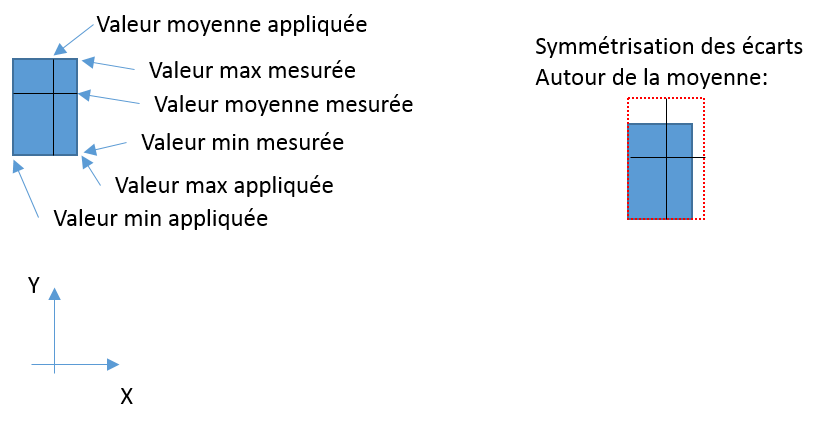
\includegraphics[width=12cm]{assets/figures/3_3_explications.PNG}
    \caption{Un point de mesure, avec les incertitudes sur la valeur appliquée X et sur la valeur mesurée Y.}
    \label{fig:3_3_explications}
\end{figure}

\begin{figure}
    \centering
    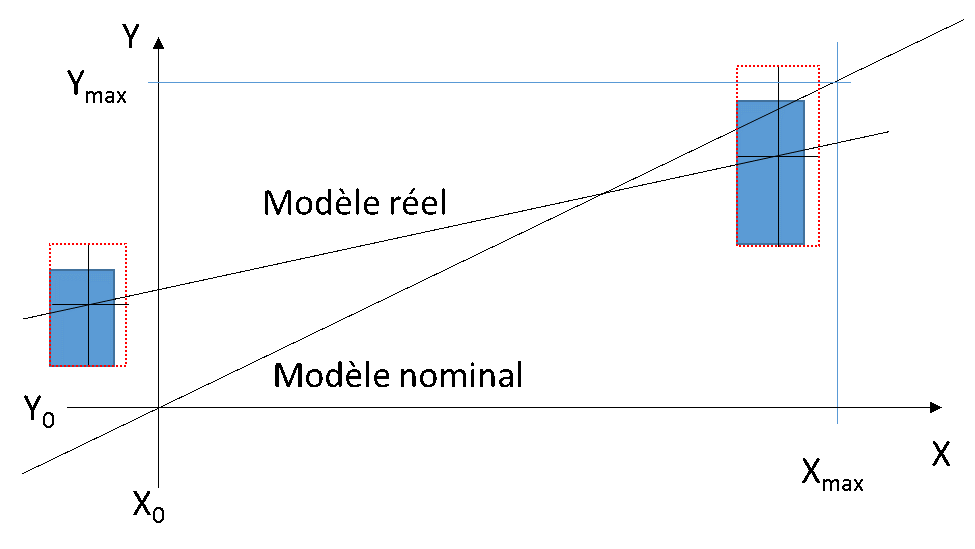
\includegraphics[width=12cm]{assets/figures/3_3a_reel_versus_nominal.PNG}
    \caption{Mesure après calibrage: modèles nominal et réel.}
    \label{fig:3_3a_reel_versus_nominal}
\end{figure}

\begin{figure}
    \centering
    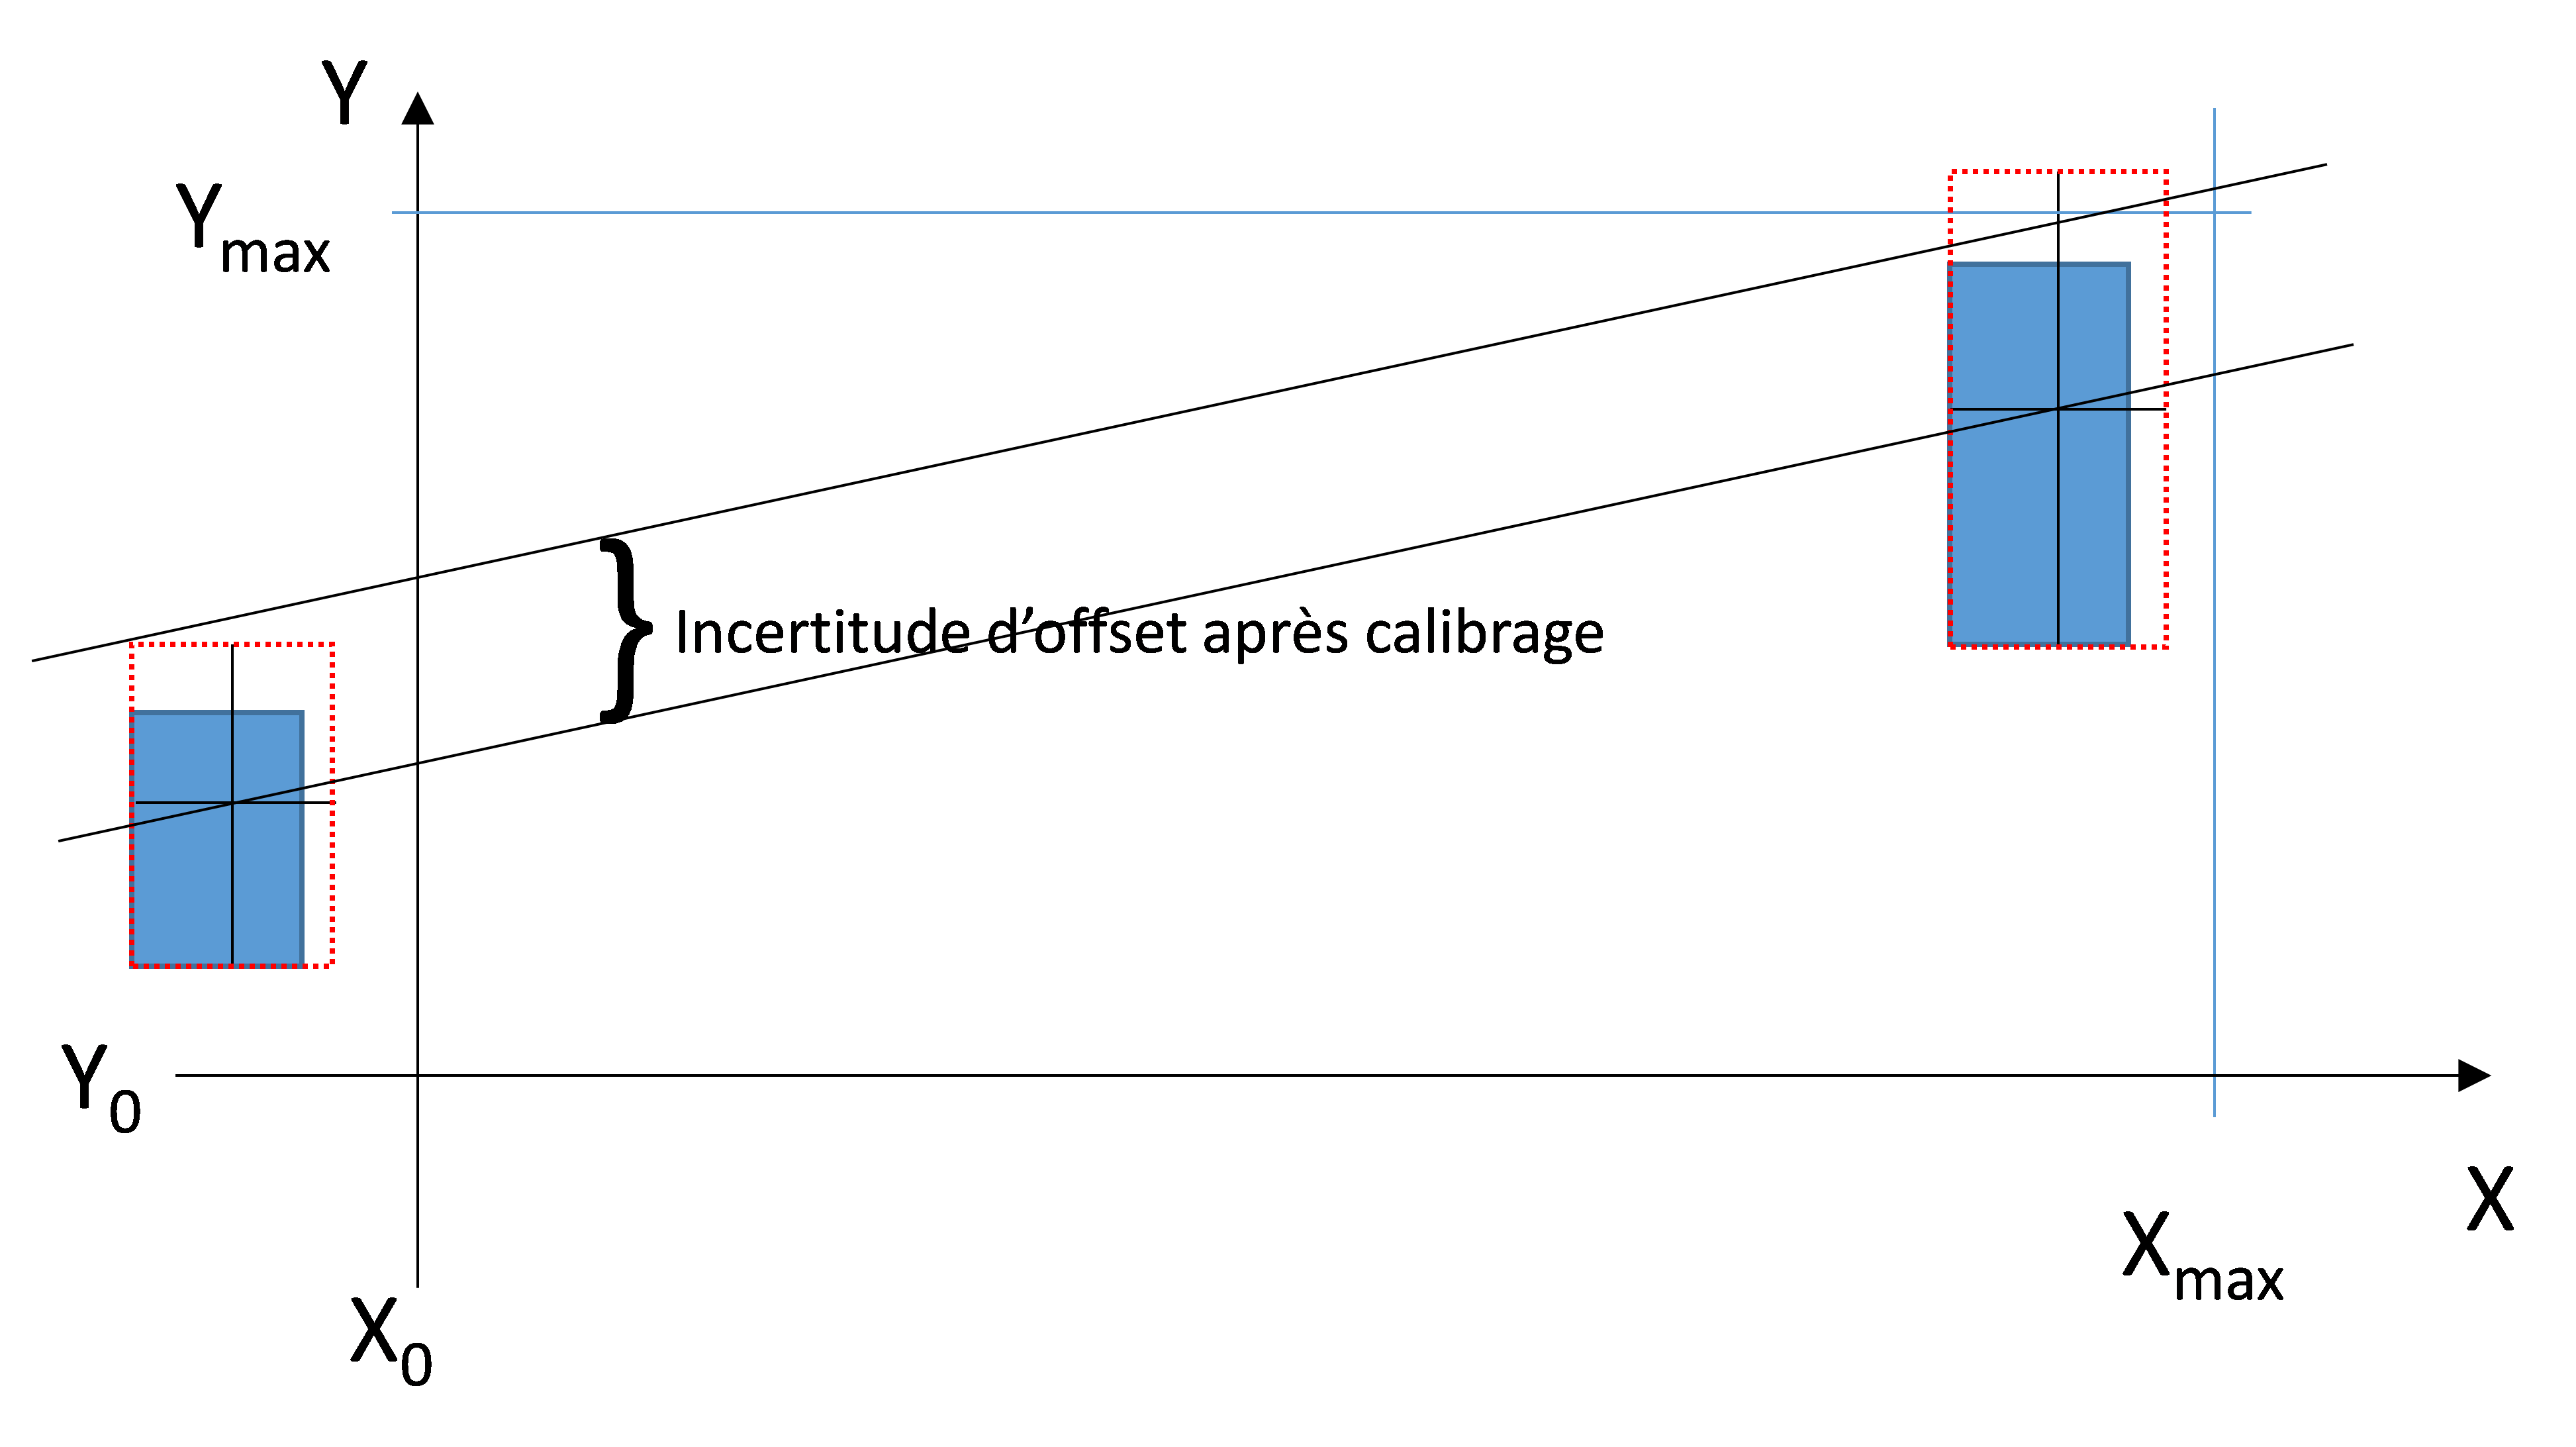
\includegraphics[width=12cm]{assets/figures/3_3b_incertitude_de_offset.PNG}
    \caption{Mesure après calibrage: incertitude sur l'offset.}
    \label{fig:3_3b_incertitude_de_offset}
\end{figure}

\begin{figure}
    \centering
    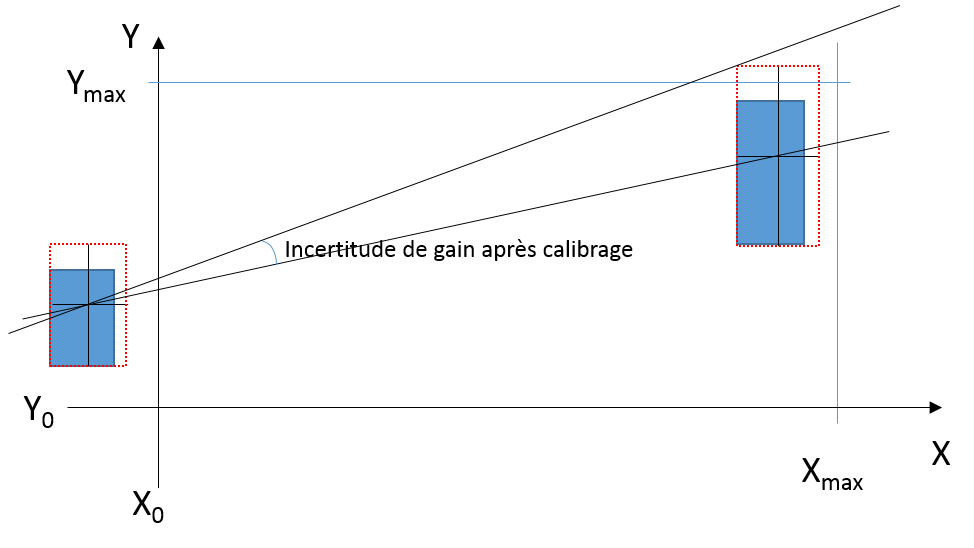
\includegraphics[width=12cm]{assets/figures/3_3c_incertitude_de_gain.PNG}
    \caption{Mesure après calibrage: incertitude sur le gain.}
    \label{fig:3_3b_incertitude_de_gain}
\end{figure}

En résumé, le calibrage consiste à :

\begin{center}
    \fbox{
        \begin{minipage}{0.96\textwidth}
            \textbf{ }
            \begin{itemize}
                \item Imposer un mesurande $X_0$ nul correspondant au zéro de mesure, et ajuster le décalage de la chaîne pour obtenir l'offset du modèle nominal ; le zéro est le point sur lequel le gain n'a pas d'effet.
                \item Imposer la valeur maximum $X_{max}$ de mesure et ajuster le gain (span) de la chaîne pour obtenir la valeur correspondante selon le modèle nominal.
                \item Déterminer les incertitudes sur les valeurs ajustées et en déduire les incertitudes de calibrage:	$D_{c} = \Delta X_{o} + \frac{\Delta Y_{o}}{G} $ et
                      $\alpha _{c} = \frac{D_{c} + \Delta X_{max} + \frac{\Delta Y_{max}}{G}}{X_{max} -X_{o}} $
            \end{itemize}
        \end{minipage}
    }
\end{center}

Après une opération de calibrage, on peut généralement considérer que les erreurs de gain et de décalage ont été annulées. Par conséquent, pour les mêmes valeurs des grandeurs d'influence (raisonnablement quelques minutes à quelques heures après le calibrage) seules interviennent les erreurs de non-linéarité et le bruit interne. C'est pourquoi un calibrage préalable est très souvent utilisé dans les procédures de mesure. Dans ce cas on utilisera comme référence le modèle nominal.

Dans certains cas, lorsque les moyens de réglage ne nous permettent pas de nous rapprocher suffisamment du modèle nominal ou lorsqu'on cherche à améliorer la précision, alors on choisira comme référence le modèle réel obtenu par étalonnage, mesuré après calibrage. Dans ce dernier cas, alors les valeurs $\Delta X_{o}$ et $\Delta Y_{o}$ ainsi que $\Delta X_{max}$ et $\Delta Y_{max}$ seront généralement établies autour des valeurs moyennes de $\Delta X$ et $\Delta Y$.

Lorsqu'il n'est pas possible ou pas souhaitable d'appliquer un mesurande nul, l'évaluation des incertitudes suivra le même principe que ci-dessus, mais il faudra tenir compte du fait que chacun des points $X_{min}$ et $X_{max}$ influencent la réponse à $X_{0}$, et donc la valeur du décalage. Les relations pour $D_{c}$ et $\alpha_{c}$ ne sont alors pas valables.

\subsection{Étalonnage}

Ici, il faut établir un tableau de mesure, couvrant toute l'étendue de mesure. Manuellement on se contente d'une dizaine de mesures répartie entre le minimum et le maximum. Lorsqu'on utilise un système d'acquisition, on recherche un beaucoup plus grand nombre de mesures, couvrant plusieurs cycles sur l'étendue de mesure, de manière à permettre la mise en évidence de phénomènes éventuels tels que l'hystérèse, la répétabilité ou le bruit de mesure.

Pour chaque couple mesuré $(X(i), Y(i))$, on peut déterminer l'erreur
\[
    e(i) = X_m(i) - X(i) = \frac{Y(i) - Of_{nom}}{G_{nom}}   -X(i)
\]
mais ceci ne nous permet pas de bien séparer les composantes de l'erreur.

Il convient donc de déterminer le modèle actuel de la chaîne, c'est-à-dire $G_{réel}$ et $Of_{réel}$, après quoi on pourra séparer les composantes d'erreur (gain, décalage, non-linéarité et bruit). La manière de définir la droite de réponse influence quelque peu les résultats, si bien qu'il est indispensable d'utiliser une définition commune, si l'on veut comparer les résultats (par exemple avec les spécifications individuelles des composants de la chaîne). On utilise généralement deux méthodes de choix de cette droite:
\begin{center}
    \fbox{
        \begin{minipage}{0.96\textwidth}
            \textbf{Droite par les extrêmes (End points linearity) :}
            la droite passe par deux points de la courbe de réponse réelle (en général le zéro et la pleine échelle, ou encore les deux extrémités du domaine de mesure).\\

            \textbf{Meilleure droite (Best fit linearity) :}
            C'est la droite de régression linéaire, elle minimise la somme des carrés des écarts entre la courbe de réponse réelle et la droite ainsi définie.
        \end{minipage}
    }
\end{center}

Le gain réel $G_{reel}$ est la pente de la droite ainsi choisie. Le décalage réel $D_{reel}$ est l'ordonnée à l'origine de la droite. Pour chaque couple mesuré $(X(i),Y(i))$ on détermine l'écart entre la valeur mesurée et la droite $\Delta = Y(i) - [G_{reel}\cdot X(i) + Of_{reel}]$. Cet écart est une combinaison de l'erreur de non-linéarité et du bruit. Pour une utilisation immédiate après le calibrage, cet écart représente l'erreur résiduelle du montage, et on en spécifie la limite maximum en valeur absolue, dans l'unité du mesurande, ce qui revient à diviser $max{|\Delta|}$ par le gain de la chaîne:
\[
    NL+Bruit = \frac{max{|\Delta|}}{G_{reel}}
\]
Une séparation du bruit et de la non-linéarité n'est généralement pas nécessaire.
Les erreurs de gain et de décalage du modèle réel par rapport au modèle nominal se calculent en comparant $G_{reel}$ et $Of_{reel}$ avec $G_nom$ et $Of_nom$ :

\[\alpha =  \frac{G_{reel}-G_{nom}}{G_{nom}}	 \]
\[D =  \frac{Of_{reel}-Of_{nom}}{G_{nom}} \]

Dans certains cas on sera amené à établir les incertitudes de gain et de décalage du modèle réel par rapport à lui-même, dues à des instabilités constatées sur l'affichage et à des difficultés d'appliquer un mesurande parfaitement stable. Dans ce cas on procédera comme au point précédent pour l'établissement des incertitudes de calibrage.

\subsection{Auto calibrage }
Les avantages apportés par un calibrage juste avant une série de mesures sont tels qu'il devient indispensable de le réaliser pour compenser les effets des grandeurs d'influence si l'on veut atteindre une haute précision. C'est pourquoi de nombreux équipements de précision incorporent une séquence automatique de calibrage (ou au moins d'ajustage du zéro = auto zéro) à intervalles réguliers ou même avant chaque mesure. Ce calibrage peut se faire de manière analogique ou entièrement numérique.
Pour permettre un auto calibrage, il suffit d'insérer un commutateur permettant de déconnecter l'entrée normale de mesure pour la remplacer par les étalons correspondants à $X_0$ et à $X_{max}$. La séquence de travail lors du calibrage est semblable à la séquence manuelle, si ce n'est qu'il faut mémoriser les valeurs de correction. Ensuite, il faut soit agir sur les réglages matériels, soit utiliser un moteur de correction, qui n'est en fait rien d'autre qu'un calculateur. Si ce calculateur se trouve dans la chaîne de mesure et que celle-ci fournit une sortie numérique ainsi calibrée, alors on a bien un auto calibrage. Toutefois dans certains cas la chaîne de mesure fournit d'une part le signal sans correction, d'autre part les paramètres de correction. Dans ce dernier cas, on parlera alors d'auto étalonnage.

\section{Compensation des erreurs systématiques}

Au lieu d'un auto calibrage, il est parfois plus efficace de faire une compensation directe d'une erreur systématique, s'il est possible d'identifier son influence. Un cas typique se présente dans les capteurs de pression intégrés où la température est l'influence prépondérante ; souvent c'est également l'influence de la tension d'alimentation qu'il faut pouvoir compenser.

\subsection{Compensation linéaire }
L'identification consiste à déterminer les coefficients d'influence agissant sur le gain et le décalage de la chaîne. Généralement on se contente de déterminer $G_r$ et $Of_r$ aux deux valeurs extrêmes d'utilisation. En faisant l'hypothèse que l'évolution du gain et celle du décalage sont linéairement dépendantes de la grandeur d'influence, on définit les coefficients d'influence :

\begin{center}
    \fbox{
        \begin{minipage}{0.96\textwidth}
            \textbf{\textit{Déf}. Coefficient d'influence sur le gain : }
            variation relative du gain par unité de la grandeur d'influence. Représente l'erreur de gain additionnelle due à la grandeur d'influence $Z_i : d\alpha / dZ_i = (dG_r/G_r)/dZ_i$ (proportionnelle à X : exprimée en$ \%/unité de Z_i$)
            \\
            \\
            \textbf{\textit{Déf}. Coefficient d'influence sur le décalage :}
            variation d'offset par unité de la grandeur d'influence. Représente l'erreur de décalage additionnelle due à la grandeur d'influence $Z_i$ : \\
            \begin{equation}
                {dD}{dZ_i} = \frac{(dOf_r/G_r)}{dZ_i}\text{ }[\frac{unites de X}{unites de Z_i}]
            \end{equation}
        \end{minipage}
    }
\end{center}

Pour effectuer la correction, il suffit alors de mesurer $Z_i$ (chaîne auxiliaire), d'en déduire la variation par rapport à la valeur de $Z_i$ au moment du calibrage, et de multiplier les coefficients d'influence par cet écart pour connaître la variation de gain ou de décalage par rapport au calibrage.

À titre d'exemple, prenons un capteur de pression intégré. La grandeur d'influence est la température T. On commence par étalonner le capteur aux deux températures extrêmes d'utilisation, ici environ 25 et 60 \degre C. Une telle mesure est présentée sur le graphique ci-dessous.

\begin{figure}
    \centering
    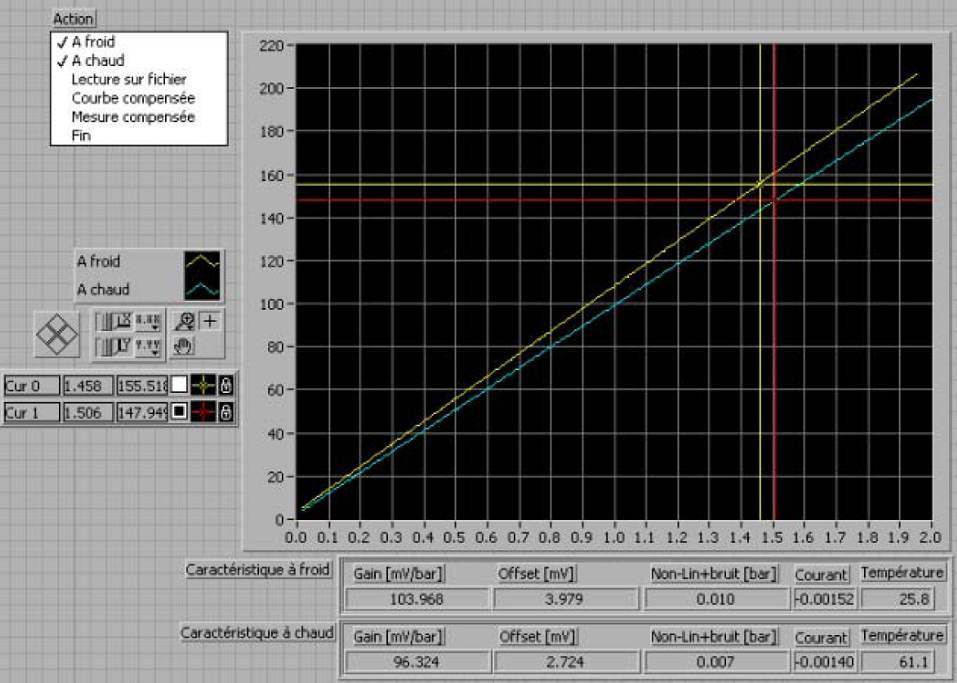
\includegraphics[height=10cm]{assets/figures/3_5_identification_reponse_en_temperature.PNG}
    \caption{ Identification de la réponse du capteur aux températures extrêmes.}
    \label{fig:IdentificationTemperature}
\end{figure}

On en déduit les coefficients d'influence, en prenant les valeurs exactes mesurées à une température de calibrage, ici 25.8 \degre C :
Gain:
\[
    \frac{d\alpha}{dT} = \frac{dGr/Gr}{dT} = \frac{(96.324-103.968)/103.968}{ (61.1-25.8)} =\]
\begin{equation}
    = \frac{-0.0735}{35.3} = -0.002083 = -0.21 \% \text{/ \degre C}
\end{equation}

Décalage:
\begin{equation}
    \frac{dD}{dT} = \frac{(dOfr/Gr)}{dT} = \frac{(2.724-3.979)/103.968}{(61.1-25.8)} =
    \frac{-0.012 bar}{ 35.3 \text{\degre C}} = -0.34 \text{mbar/ \degre C}
\end{equation}

Par conséquent, si l'on mesure alors que la température est de 38.0 \degre C, nous avons un écart de température de (38.0 - 25.8) = 12.2 \degre C et les erreurs additionnelles de gain et de décalage par rapport aux valeurs de calibrage (gain 103.968 mV/bar et offset 3.979 mV) seront de :

$d\alpha = -0.002083 \cdot 12.2 = -0.0254 = -2.54 \% lect $
\\
$dD = -0.34 m \cdot 12.2 = - 4.148 mbar $

Pour corriger les indications, il est généralement plus simple de calculer le gain et l'offset actuels avant de traduire la sortie (mV) en valeurs de pression :

$G(38 \text{\degre C}) = G(25.8 \text{\degre C}) (1 + d \alpha) = 103.968(1-0.0254) = 101.327 mV/bar $
\\
\\
$Of(38 \text{\degre C}) = Of(25.8 \text{\degre C}) + G(25.8 \text{\degre C}) \cdot dD = 3.979 - 4.148 \cdot 10-3 \cdot 103.968 = 3.548 mV$
\\

Ainsi une sortie de 89 mV correspond à une pression de (89-3.548) / 101.327 = 0.843 bar.

Sans correction, avec les valeurs de calibrage on obtient 0.731 bar : on sous-évalue la pression, car la température introduit un décalage négatif de -4.2 mbar ainsi qu'une erreur de gain négative de -2.54\% de 731 mbar soit -15.6 mbar, et donc un total de -19.8 mbar.

\subsection{Moteur de correction mathématiques}

La puissance de calcul des microprocesseurs incorporés aux capteurs dits \textless\textless\ intelligents \ \textgreater\textgreater permet d'envisager des corrections bien plus efficaces, qui sont maintenant incorporées dans les profils d'utilisation de ces capteurs (réseau de terrain).
À titre d'exemple, la norme IEEE-1451 / Smart Transducers, définit une fonction multi - variables, de type polynomial, et décomposable par segments :

\begin{equation}
    \displaystyle\sum_{i=0}^{D(1)}
    \displaystyle\sum_{j=0}^{D(2)} \text{...}
    \displaystyle\sum_{p=0}^{D(n)} C_{i,j,...,p} [X_1-H_1]^i[X_2-H_2]^j \text{...} [X_n-H_n]^p
\end{equation}

Le calcul de correction ci-dessus représente une somme polynomiale de n variables, dont on peut choisir indépendamment les degrés de chaque variable. Dans le cas de la compensation linéaire de température, nous aurions $X_1$ = sortie en mV du capteur de pression, $X_2$ = sortie du capteur de température, les degrés D(1) et D(2) seraient tous deux égaux à 1 (linéaire), et la formule permet de calculer la valeur de pression. Par conséquent la formule de calcul devient :
\begin{equation}
    P_m =C_{00} + C_{10} \cdot (X_1-H_1)+C_{01} \cdot (X_2-H_2) + C_{11}\cdot(X_1-H_1) \cdot (X_2-H_2)
\end{equation}

\begin{equation*}
    = C_{00} + C_{01} \cdot X_2 + X_1 \cdot (C_{10} + C_{11} \cdot X_2)  \text{ si les termes $H_1$ et $H_2$ sont nuls }
\end{equation*}

On voit bien qu'ainsi on a bien un décalage $(C_{00} + C_{01} \cdot X_2)$ dépendant de $X_2=T$ et un gain $(C_{10} + C_{11} \cdot X_2)$ également dépendant de T. Par contre cette méthode permet des corrections bien plus évoluées (polynômes et compensation de plusieurs grandeurs d'influence).

Pour de grands domaines ou pour de fortes non-linéarités, afin d'éviter des polynômes de degré trop élevé, la norme prévoit de segmenter la réponse selon les valeurs des différentes variables, et d'exploiter un ensemble de paramètres de faible degré dans chaque segment, comme illustré dans la figure ci-dessous.

\begin{figure}
    \centering
    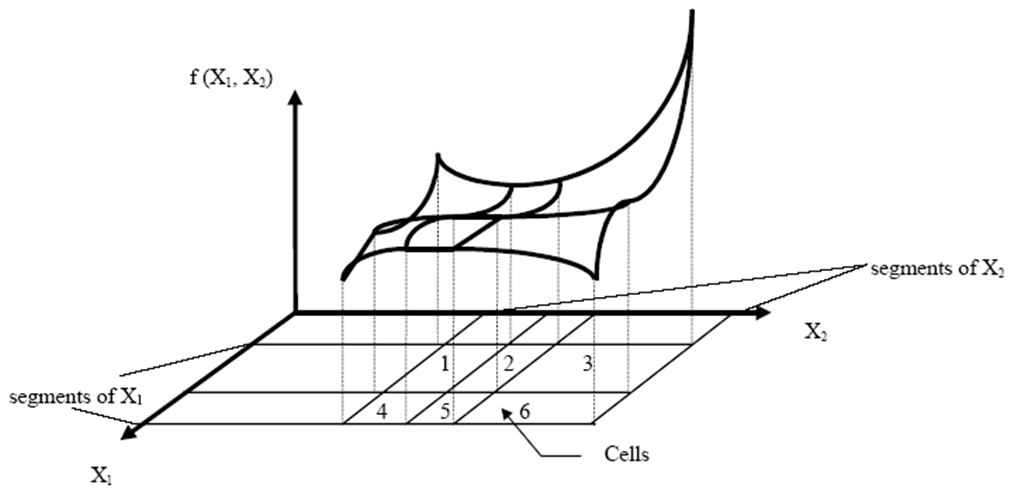
\includegraphics[height=6cm]{assets/figures/3_6_Correction_a_2_variables_segementees.PNG}
    \caption{Correction à deux variables segmentées.}
    \label{fig:Correction_a_2_variables_segementees}
\end{figure}

A chaque élément de surface (désigné par "Cell") correspond un ensemble de paramètres $C_{ij}$ et $H_x$ permettant d'approcher la surface réelle en minimisant le nombre total de paramètres à mémoriser.

\section{Mesures répétées}

Lors de mesures répétées de la même valeur du mesurande X, on constate que les résultats ne sont pas toujours parfaitement ceux qu'on attend, et ne sont pas identiques. Une analyse statistique des résultats de mesure permettra d'établir une valeur moyenne $\mu$ de tous les résultats ainsi qu'un écart-type $\sigma$. Les mesures sont en général réparties autour de la moyenne selon une distribution gaussienne caractérisée par cet écart-type. Ainsi la moyenne constitue la partie systématique de l'erreur appelée aussi le biais, alors que l'écart-type représente sa composante aléatoire.

\newpage
On a donc :
\begin{itemize}
    \item X, le mesurande
    \item La moyenne des mesures $\mu$
    \item L'erreur de biais $\beta :  \beta = \mu - X$  [unité de X], erreur systématique
    \item L'exactitude ou la justesse, termes utilisés pour caractériser l'erreur systématique
    \item L'écart-type $\sigma$ sert à quantifier l'erreur aléatoire
    \item La répétabilité ou la fidélité, termes utilisés pour caractériser l'erreur aléatoire
\end{itemize}

\begin{equation}
    \mu = \lim\limits_{N \to \infty} \frac{1}{N} \sum_{i=1}^N x_i
\end{equation}

\begin{equation}
    \sigma = \lim\limits_{N \to \infty} \sqrt{\frac{1}{N}\sum_{i=1}^N (x_i-\mu)^2}
\end{equation}

\begin{figure}
    \centering
    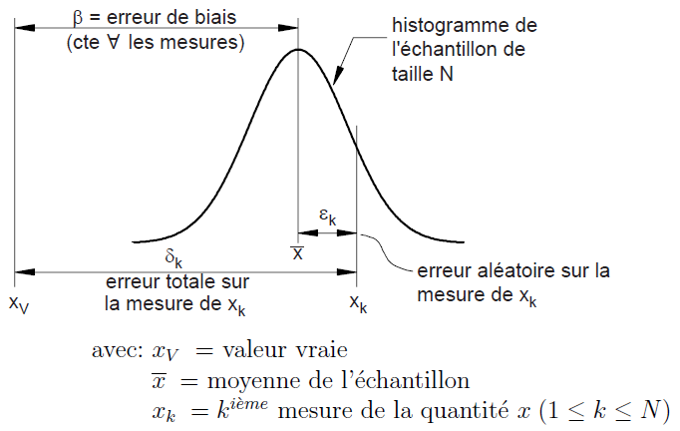
\includegraphics[height=7cm]{assets/figures/3_7_Exemple_de_mesures_repetees_N_fois.PNG}
    \caption{Exemple de mesures répétées N fois, où N >100 pour être significatif.}
    \label{fig:Exemple_de_mesures_repetees_N_fois}
\end{figure}

\begin{figure}
    \centering
    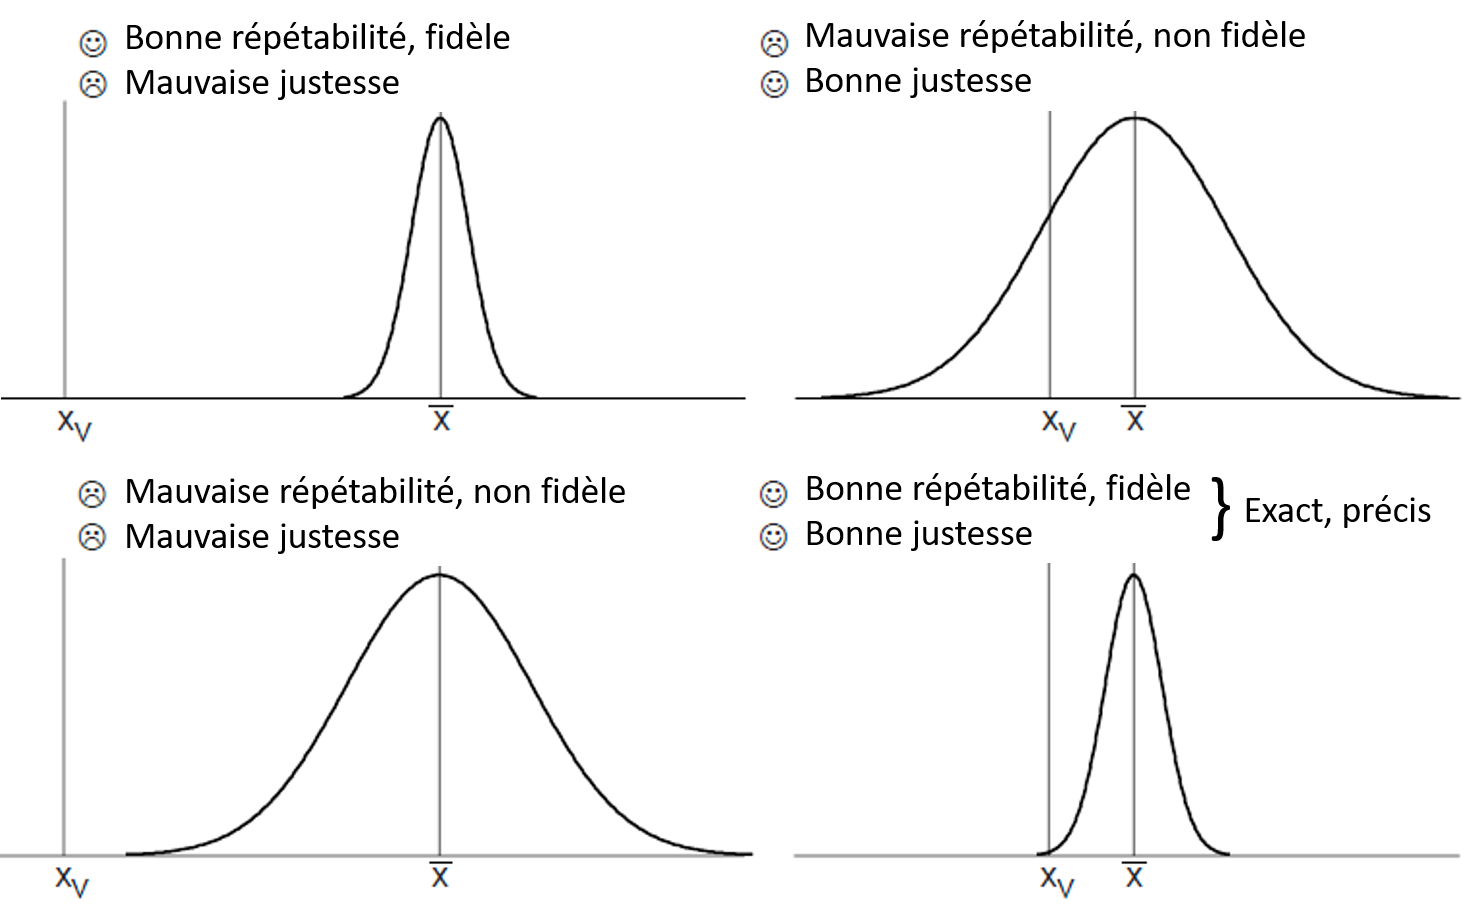
\includegraphics[height=7cm]{assets/figures/3_8_distinction_entre_repetabiite_et_justesse.PNG}
    \caption{distinction entre répétabilité et justesse.}
    \label{fig:distinction_entre_repetabiite_et_justesse}
\end{figure}

\begin{figure}
    \centering
    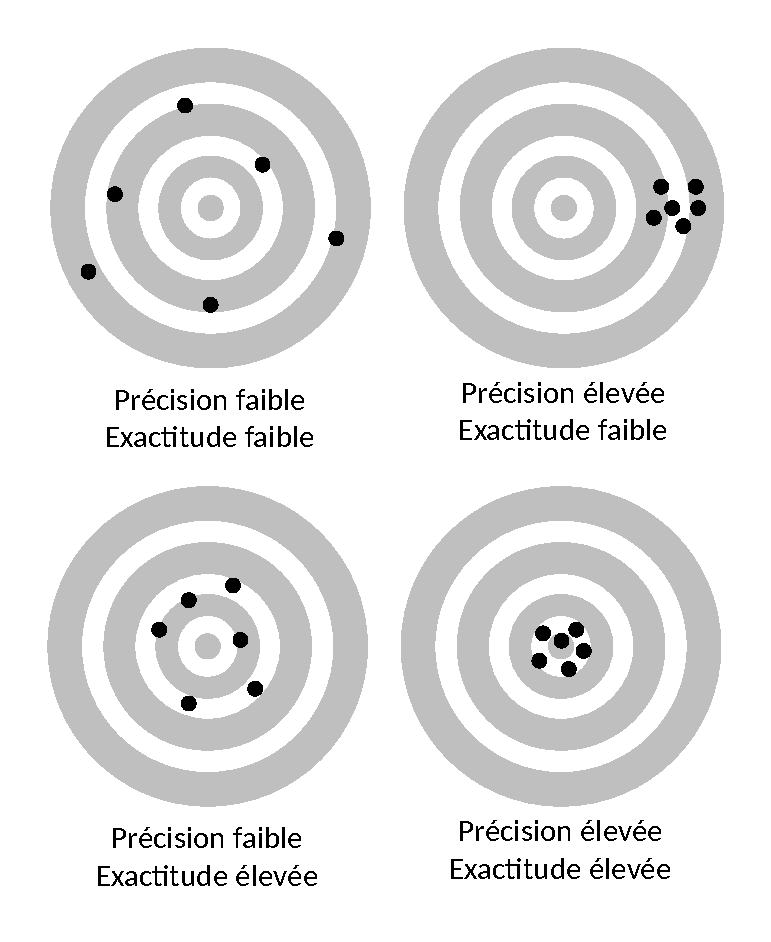
\includegraphics[height=7cm]{assets/figures/juste-fidèle-précis.pdf}
    \caption{Autre représentation des notions de justesse et fidélité.}
    \label{fig:juste_fidele_precis}
\end{figure}

L'écart-type sert à mesurer la dispersion d'un ensemble de données. Plus il est faible, plus les valeurs sont regroupées autour de la moyenne. Par exemple pour la répartition des notes d'une classe, plus l'écart type est faible, plus la classe est homogène. ¿ l'inverse, s'il est plus important, les notes sont moins resserrées. Dans le cas d'une notation de 0 à 20, l'écart-type minimal est 0 (notes toutes identiques), et peut valoir jusqu'à 10 si la moitié de la classe a 0/20 et l'autre moitié 20/20.

En sciences, il est fréquent de considérer que les valeurs se répartissent selon une courbe de Gauss. Dans le cas des sciences sociales, par exemple, la moyenne $\mu$ et l'écart-type $\sigma$ permettent de déterminer un intervalle dans lequel on trouve une majorité de la population. En effet, si la moyenne est $\mu$ et l'écart type est $\sigma$, on trouve 95 \% de la population dans l'intervalle $[ \mu - 1.96 \sigma ; \mu + 1.96 \sigma ]$ et on trouve 68.2 \% de la population dans l'intervalle $[ \mu - \sigma ; \mu + \sigma ]$.

L'écart-type est aussi utilisé pour construire un intervalle de confiance attribuable à un échantillon. Si l'on se réfère à la figure ci-contre, on voit qu'un $\sigma$ d'écart de part et d'autre de la valeur moyenne recouvre 68,2\% de la distribution, deux $\sigma$ d'écart $(13.6+34.1+34.1+13.6 =) 95.4\%$, 3 $\sigma$ d'écart $(2.1+13.6+34.1+34.1+13.6+2.1 =) 99.6\%$ et ainsi de suite... C'est l'usage notamment en physique des particules, où la détection d'évènements est quantifiée en nombre de sigmas, et où un résultat notamment est considéré comme significatif par l'obtention de 5 $\sigma$, représentant une probabilité d'erreur inférieure à 0,00003\% (niveau de confiance de plus de 99.99997\%).

En pratique, on considère que :
\begin{itemize}

    \item $1 * \sigma \rightarrow 68\% $
    \item $2 * \sigma \rightarrow 95\% $
    \item $3 * \sigma \rightarrow 99.7\%$

\end{itemize}


\begin{figure}
    \centering
    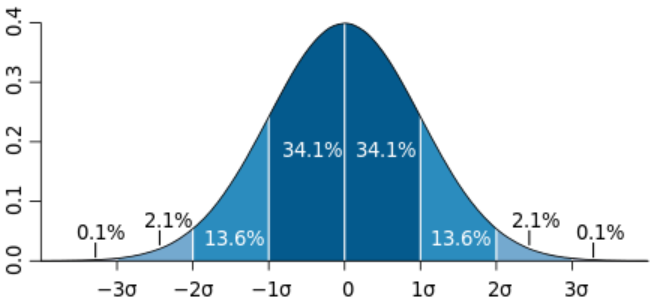
\includegraphics[height=7cm]{assets/figures/3_9_Loi_normale_et_intervale_de_confiance.PNG}
    \caption{Loi normale et intervalle de confiance.}
    \label{fig:3_9_Loi_normale_et_intervale_de_confiance}
\end{figure}

\section{Exercices }

\subsection{Exercice: Incertitudes des appareils }
Spécifications:\\
\\
\textbf{HP34401A}: spécifié pour 1 an, $23 \pm 5 \degree C$, en (\%lect+ \%gamme) et jusqu'à 20\% de dépassement de gamme\\
\\
\begin{tabular}{l c c}
    \hline
    gamme: & 100.0000 mV & 0.0050 + 0.0035 \\
           & 1.000000 V  & 0.0040 + 0.0007 \\
           & 10.00000 V  & 0.0035 + 0.0005 \\
           & 100.0000 V  & 0.0045 + 0.0006 \\
           & 1000.000 V  & 0.0045 + 0.0010 \\
    \hline
\end{tabular}
\\
\\
\textbf{Prema} 6000:spécifs pour 1 an, $23 \pm 5 \degree C$, en (\% of reading + \% of full scale)
Full scale : 1'999'999 (sauf gamme 1000 V : 1'000'000)
\\
\begin{tabular}{lcc}
    \hline
    range & $\pm$ 0.2 V  & 0.006 + 0.0007 \\
          & $\pm$ 2 V    & 0.005 + 0.0005 \\
          & $\pm$ 20 V   & 0.005 + 0.0006 \\
          & $\pm$ 200 V  & 0.005 + 0.0006 \\
          & $\pm$ 1000 V & 0.006 + 0.0005 \\
    \hline
\end{tabular}
\\
\\
\textbf{APPA-98}: spécifié pour 2 ans, $23 \pm 5 \degree C$ et moins de 75\% humidité relative, en (\% reading + number of digits)
\\
\begin{tabular}{lcl}
    \hline
    Range  & Resolution & Accuracy                     \\
    200 mV & 100 $\mu$V & |                            \\
    2 V    & 1 mV       & |                            \\
    20 V   & 10 mV      & |  $\pm$ (0.5 \%rdg + 1 dgt) \\
    200 V  & 100 mV     & |                            \\
    1000 V & 1 V        & |                            \\
    \hline
\end{tabular}
\\

\begin{enumerate}
    \item Quelles sont les incertitudes absolues et relatives si on mesure 2.2 V avec HP34401A ?
    \item Quelles sont les incertitudes absolues et relatives si on mesure 2.2 V avec APPA-98 ?
    \item Quelle est l'incertitude relative maximum si on mesure entre 10 et 250 mV avec HP34401A ?
    \item Quelle est l'incertitude relative maximum si on mesure entre 10 et 250 mV avec Prema6000 ?
    \item Quelle est l'incertitude absolue maximum si l'on mesure entre 30 et 500 V avec APPA-98 ?
    \item Représenter les incertitudes relatives du HP34401A et du Prema6000 pour un domaine de 10mV à 1000V (utilisez une échelle Log pour l'axe X des tensions).
\end{enumerate}
NB: la pleine échelle définie pour le PREMA n'est pas la définition habituelle qui dit que la pleine échelle est la différence entre les valeurs min et max. On aurait alors attendu pour le PREMA une pleine échelle égale au double de la gamme.

\subsection{Exercice: Calibrage d'une chaîne}
a)	Une chaîne de mesure de température doit être utilisée pour la régulation de température d'une enceinte, autour de 60 $\degree$ C. On désire qu'elle nous indique l'erreur (température actuelle moins consigne de 60 $\degree$ C). Le calibrage est réalisé ainsi: \\
i)	on place le capteur dans un bain à 60 $\pm$ 0.35 $\degree$ C, et on ajuste le décalage pour un affichage nominal de 0.00. On constate que les indications oscillent entre -0.03 et + 0.08. \\
ii)	on place le capteur dans un bain à 70 $\pm$ 0.5 $\degree$ C, et on ajuste le gain pour un affichage nominal de 10.00. On constate que les indications oscillent entre 9.88 et 10.09. \\  ~ \\
Quelles sont les incertitudes de gain et de décalage dues à ce calibrage ? \\

b)	Une chaîne de mesure doit indiquer l'épaisseur d'une feuille plastic (capteur capacitif sans contact, basé sur la variation de la constante diélectrique). Le calibrage s'effectue comme suit: \\
i)	Pas de feuille dans le capteur, on ajuste le décalage et on obtient un affichage stable de 000. \\
ii)	On place une feuille étalon d'épaisseur 0.500  $\pm$  0.005 mm dans le capteur, et on ajuste le gain pour un affichage nominal de 500. Malheureusement le potentiomètre ne permet pas l'ajustage exact et on doit se contenter d'un affichage oscillant entre 497 et 499. \\~ \\
Quelles sont les incertitudes de calibrage de cette chaîne ? \\

c)	Une chaîne de mesure de la hauteur du liquide contenu dans un réservoir utilise la pression relative à la base de ce réservoir (P = $\rho\,gh$ où h est la hauteur du liquide dans le réservoir). Pour le calibrage on procède comme suit: \\
i)	Réservoir vide, on ajuste le décalage pour un affichage de 0000  $\pm$  0001 \\
ii)	On remplit le réservoir, on mesure une hauteur h = 10.00 $\pm$ 0.02 m, ainsi que la densité du liquide  $\rho$ = 0.800  $\pm$  0.006 kg/dm3, et on ajuste l'affichage à 1000  $\pm$  0003 \\ ~ \\
Quelles sont les incertitudes de calibrage (indication: n'oubliez pas que la chaîne est sensible à la pression et non directement à la hauteur du liquide)? \\

d)	On a calibré un capteur de pression relative (=différence de pression par rapport à l'atmosphère) de la manière suivante : pression appliquée par une pompe dans la tuyauterie du capteur avec une vanne de détente, mesure de la pression appliquée par la différence de hauteur de mercure dans un tube en U, ouvert sur l'atmosphère, lecture de la sortie dans un PC. La réponse nominale est 0 à +2 bar, 0 à +20'000digit (1 bar = 100kPa). \\
i)	Vanne ouverte (= pression atmosphérique), ajustage de l'offset pour une valeur nominale de 0, on obtient un affichage stable de 00'000digit. \\
ii)	Vanne fermée, on agit sur la pompe jusqu'à une hauteur de mercure de 148.5 $\pm$ 0.2cm dans le tube en U. On calcule alors la pression appliquée $P=\rho\,gh = 13.6\times10^3 \text{ kg/m}^3 * 9.81\text {m/s}^2 * 1.485\text{ m}=198.12276\text{ kPa} = 1.98123\text{ bar}$. On ajuste donc le gain pour obtenir un affichage nominal de 19'812.3 digit, et obtient un affichage oscillant entre 19'810 et 19'814. \\ ~\\
Quelles sont les incertitudes de calibrage ?

\subsection{Exercice: Linéarité}

a)On a mesuré la réponse d'un capteur de force à $23 \degree C$ (réponse idéale : $0-100N \Leftrightarrow 0-20 mV$):\\
~
\\
\begin{tabular}{|l|l|l|l|l|l|l|l|l|l|l|l|}
    \hline
    F [N]  & 0    & 10   & 20   & 30   & 40   & 50    & 60    & 70    & 80    & 90    & 100  \\
    \hline
    U [mV] & 0.50 & 2.49 & 4.46 & 6.41 & 8.34 & 10.25 & 12.14 & 14.01 & 15.86 & 17.69 & 19.5 \\
    \hline
\end{tabular}
\\

Déterminez l'offset réel en [mV], le gain réel en [mV/N], les erreurs de décalage [N], de gain [\%lect] et l'incertitude de non-linéarité en [N] et en [\%(PE)] de ce montage par les deux méthodes :
\begin{enumerate}
    \item Choix de la droite de référence par les extrémités de la courbe de réponse
    \item Choix de la "meilleure droite"	 ...
\end{enumerate}
~\\

b)	L'étalonnage d'une chaîne de mesure de couple, gamme 0 à 100 mNm, sortie 4 à 20 mA, a donné: \\
~
\\
\begin{tabular}{|l|l|l|l|l|l|l|l|l|l|l|l|}
    \hline
    \footnotesize C [mNm] & 0                    & 10                   & 20                   & 30                   & 40                    & 50                    & 60                    & 70                    & 80                    & 90                    & 100                   \\
    \hline

    \footnotesize I [mA]  & \footnotesize  3.960 & \footnotesize  5.564 & \footnotesize  7.192 & \footnotesize  8.800 & \footnotesize  10.443 & \footnotesize  12.063 & \footnotesize  13.677 & \footnotesize  15.315 & \footnotesize  16.926 & \footnotesize  18.550 & \footnotesize  20.160 \\
    \hline
\end{tabular}
\\

L'équation nominale de cette chaîne vaut donc $I = 4 [mA] + 0.16 [\frac{mA}{mNm}]  \cdot C [mNm]$.

Quelles sont les erreurs de gain et de décalage ainsi que l'incertitude de non-linéraité + bruit dans les 2 cas suivants:
\begin{enumerate}
    \item Choix de la droite de référence par les extrémités de la courbe de réponse
    \item Choix de la "meilleure droite"	 ...
\end{enumerate}

\subsection{Exercice: Auto-Calibrage d'une chaîne}

a)	Pour réaliser l'auto calibrage d'un canal de mesure de courant (nominal 0-20 mA, code numériques 0-2000 digits), on procède comme suit:
\begin{itemize}
    \item ouverture du circuit de mesure par un interrupteur (donc courant nul), mémorisation du code obtenu :  $N_0=2$ (stable)
    \item Fermeture d'un interrupteur reliant une source de tension de référence ($U_g = 10.000V \pm 0.005V$) au circuit de mesure à travers une résistance de $R_g = 500 \Omega \pm 0.1\%$ (la borne de mesure étant supposée travailler à potentiel nul, le courant nominal ainsi imposé est de 20mA). On mémorise alors le code moyen obtenu sur 10 mesures : $N_1 = 2018.3$, alors que les codes max et min sont 2021 et 2015.
    \item Les mesures seront ensuite corrigées à l'aide de $N_0$ et $N_1$ pour obtenir :
          \begin{itemize}\itemsep1pt
                    \renewcommand{\labelitemi}{$\bullet$}
              \item i) une valeur numérique corrigée ;
              \item ii) une valeur dans l'unité du mesurande ;
          \end{itemize}
\end{itemize}
NB : si ces corrections sont faites à l'extérieur de la chaîne de mesure, alors on parlera d'auto étalonnage.
Quelles sont les fonctions mathématiques de correction et quelles sont les incertitudes de calibrage ?\\

b)	Pour programmer l'auto calibrage d'une chaîne de mesure de température dont le capteur (PT100 : $R(T)=100 \Omega (1+0.00385T)$ a une interchangeabilité de 0.2 $\degree$ C + 0.1\%lecture, on a inséré des interrupteurs programmables permettant de déconnecter le capteur et de le remplacer soit par une résistance de$ 100 \Omega \pm 0.1 \Omega$, soit par une résistance de $138.5 \Omega \pm 0.14 \Omega$. La séquence d'auto calibrage est la suivante :
\begin{itemize}
    \item Capteur remplacé par la résistance de $100 \Omega$, on mémorise la moyenne de 100 conversions: on trouve $M_0=1985.65$, toutes les conversions sont soit 1985, soit 1986.
    \item Capteur remplacé par la résistance de $138.5 \Omega$. On mémorise la moyenne de 100 conversions: $M_1=2825.45$, conversion maximum 2827, minimum 2824.
    \item Pour les mesures, on ne fait qu'une seule conversion $N_x$, et l'on calcule \\
          $T= (N_x - M_0)\frac{100}{M_1 - M_0}$
\end{itemize}
Quelles sont les incertitudes de calibrage ? \\

c)	Une chaîne de mesure de pression est constituée d'un capteur-transmetteur avec les spécifications suivantes : gamme -1 à +3 bar, sortie 4 à 20mA, précision 0.5\%lect + 35 mbar ; le courant de sortie est mesuré par une résistance shunt de $10 \Omega \pm 0.012 \Omega$, et un convertisseur gamme $\pm 0.25V$.
Pour programmer l'autocalibrage de cette chaîne, on a inséré des interrupteurs programmables permettant de déconnecter le capteur et de le remplacer soit en laissant le circuit ouvert, soit en reliant une résistance de $490 \Omega \pm 0.2 \Omega$ entre la borne positive du shunt et une source de tension de $+10V \pm 15mV$ (courant nominal de 20 mA). La séquence d'auto calibrage est la suivante :
\begin{itemize}
    \item Capteur déconnecté, circuit ouvert on mémorise la moyenne de 100 conversions: on trouve $M_0=-0.73$ digit, toutes les conversions sont soit -1, soit 0 digit.
    \item Capteur déconnecté, résistance $490 \Omega$ enclenchée. On mémorise la moyenne de 100 conversions: $M_1=1647.32$, conversion maximum 1646, minimum 1649 digit.
    \item Les valeurs de $M_0$ et $M_1$ nous permettent de calculer le gain et l'offset total actuel de la chaîne.
\end{itemize}

Quelles sont les incertitudes de calibrage ?

\subsection{Exercice: Coefficients d'influence}

a)	On a étalonné une chaîne de mesure de position à deux températures:


\begin {center}
\begin{tabular}{lll}
    $T_1=25 \degree C$ & $G_1= 100.3 digit/mm$  & $Of_1 = 3.4 digit$  \\
    $T_2=75 \degree C$ & $G_2 = 103.5 digit/mm$ & $Of_2 = -5.8 digit$ \\
\end{tabular}
\end{center}
~\\
\begin{itemize}
    \item Déterminer les coefficients d'influence de la température
    \item A une température de 40 $\degree$ C, l'indication obtenue est de 1380 digit. Calculer la position correspondante
\end{itemize}
~\\


b)	Une chaîne de mesure du contenu d'un réservoir utilise un capteur de force à jauges de contraintes (pont de Wheatstone à 4 jauges)

\begin{figure}[h!]
    \centering
    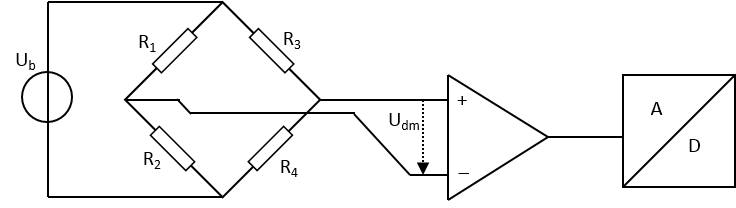
\includegraphics[height=3.7cm]{assets/figures/Exercice_3_5_c.PNG}
    \caption{Chaîne de mesure du contenu d'un réservoir.}
    \label{fig:Exercice_3_5_c}
\end{figure}

\begin{center}
    $R_1 = R_4 = R_0(1 + F \cdot K)$\\
    $R_2 = R_3 = R_0(1 - F \cdot K)$\\
\end{center}

Avec K = facteur de jauge et F = force appliquée.\\

On en déduit :	$U_{dm} = U_b ( \frac{ R_4}{R_3+R4} - \frac{R2}{R1+R2} ) = U_b \frac{ Ro(1+KF) -Ro(1-KF)}{2Ro}  = Ub \cdot K \cdot F$ \\
La sortie est donc théoriquement proportionnelle à la force, mais aussi à la tension d'alimentation $U_b$, on parle alors de capteur ratio-métrique : la sortie est une fraction (ratio) de l'alimentation.

On a étalonné la chaîne dans les 3 conditions suivantes :\\

\begin {center}
\begin{tabular}{llll}
    $U_b = 5V$ & $T=25 \degree C$ & $G_1 = 1015 digit/tonne$ & $Of_1 = -55 digit$ \\
    $U_b = 3V$ & $T=25 \degree C$ & $G_2 = 609 digit/tonne$  & $Of_2 = -33 digit$ \\
    $U_b = 5V$ & $T=50 \degree C$ & $G_3 = 1095 digit/tonne$ & $Of_3 = +12 digit$ \\
\end{tabular}
\end{center}
~\\
On suppose les influences indépendantes et linéaires

\begin{itemize}
    \item Calculer les coefficients d'influence de la température T et de l'alimentation $U_b$.
    \item Calculez le gain et l'offset pour une température $T=30 \degree C$ et une alimentation $U_b=5.5V$
    \item Enumérez les coefficients du moteur de correction IEEE1451
\end{itemize}

\subsection{Exercice: Mesures répétées}

Un expérimentateur utilise un capteur de pression différentielle dont on lui a dit que la plage de précision était de $\pm 2\%$, pour une différence de pression de 20 Pa, pour un intervalle de confiance de 95\%. Afin de vérifier cette affirmation, il étalonne le capteur en effectuant 100 mesures de la tension U donnée par le capteur lorsque la pression différentielle est p = 20 Pa (il contrôle cette pression de façon très précise). À partir de son échantillon de 100 mesures, il calcule $\mu = 5V$ et $\sigma = 0.2 V$. Il prétend que le capteur n'est pas aussi précis qu'on le lui avait certifié. Pourquoi?

    \chapter{Capteurs}
\label{chap:sensors}

\section{Classification des capteurs}
\subsection{Introduction}
Les capteurs peuvent être classés selon différents critères, à savoir :
\begin{itemize}
\item Principe de fonctionnement passif ou actif
\item Type de mesure absolue ou relative
\item Les types de matériaux utilisés
\item Les principes de mesures
\item Les stimuli utilisés
\item Les champs d'application
\end{itemize}

Dans ce chapitre nous listerons les critères de classement et nous présenterons quelques exemples de capteurs au travers de leur fiche de spécification.
Et n'oubliez pas le système mksA (mètre, kilogramme, seconde, Ampère, ...) ou système international d'unités de mesure vu précédemment. Le tableau \ref{fig:Systeme_international_d_unites_SI} donne un bref rappel des 7 unités physiques de base indépendantes.

\begin{figure}[h!]
\centering
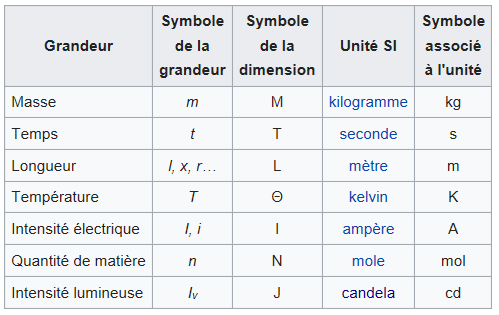
\includegraphics[height=6cm]{assets/figures/4_1_2_Systeme_international_d_unites_SI.PNG}
\caption{Système international d'unités SI: les 7 unités physiques de base.}
\label{fig:Systeme_international_d_unites_SI}
\end{figure}

\section{Choix d'un capteur}

Le choix du capteur approprié dépend du cahier des charges. Les conditions imposées sur la valeur à mesurer imposent des caractéristiques métrologiques sur le capteur.
\begin {center}
\begin{tabular}{|p{6cm}|p{6cm}|}\hline
\textbf{MESURANDE} & \textbf{CAPTEUR} \\
Conditions imposées & Caractéristiques métrologiques \\\hline\hline
Plage de variation &	Étendue de mesure \\\hline
Variation minimale à mesurer & Résolution \\\hline
Spectre de fréquence ou vitesse de rotation  & Bande passante \\\hline
Précision de mesure	& Erreur de linéarité, Erreur d'hystérésis \\\hline
Plage de température de fonctionnement &	Dérive thermique du zéro, Tenue en température \\\hline
Localisation &	Encombrement \\\hline
Composition de l'atmosphère	 & Inertie chimique, Protection \\\hline
Parasites &	Blindage, Isolement ou non par rapport à la masse \\\hline
\end{tabular}
\end{center}
Source : www.geea.org

Ces conditions concernent autant le paramètre à mesurer (par exemple la pression) que l'environnement de mesure. Elles doivent être traduites en caractéristiques métrologiques du capteur. Ces caractéristiques sont à comparer à celles se trouvant dans les fiches techniques du capteur.

Le choix du bon capteur consiste à trouver des caractéristiques qui englobent les conditions imposées sur la mesurande.

\subsection{Principaux termes utilisés pour spécifier les capteurs}

Un grand nombre de paramètres spécifient un capteur. Ces paramètres sont identifiés par les termes du tableau ci-dessous.
\begin {center}
\begin{tabular}{|p{2.2cm}|p{2.8cm}|p{6.8cm}|p{2.4cm}|}
\hline
\textbf{Français} &	\textbf{Anglais} &	\textbf{Définition} &	\textbf{exemple} \\
\hline
\hline
Sensibilité &	Sensitivity &	output variation / input variation	 & mV/g, mA/oC \\
\hline
Stabilité &	Stability &	Coefficient de variation selon une grandeur d'influence &	stabilité en température \\
\hline
Précision &	Accuracy &	Somme de toutes les perturbations qui influencent la sortie du capteur	 &  \\
\hline
Étendue de mesure &	Span, range &	Valeur max mesurable - valeur min mesurable &	  \\
\hline
Résolution &	Resolution &	Plus petite variation du mesurande mesurable par le capteur &	  \\
\hline
Sélectivité &	Selectivity &	S'applique à des capteurs biochimiques, sensibles à une molécule plus particulièrement par rapport à une autre molécule &	  \\
\hline
Temps de réponse &	Response time &	Temps de propagation entre l'entrée et la sortie du capteur &	  \\
\hline
Conditions environnementales &	Environmental conditions &	Décrit les plages de variation admissible pour les paramètres extérieurs &	humidité, température, pression \\
\hline
Facteur de surcharge &	Overload characteristics &	Capacité à supporter un dépassement de la plage de mesure du mesurande & \\
\hline
Linearité &	Linearity & &	 	  \\
\hline
Hystérèse &	Hysteresis & &	 	  \\
\hline
Zone morte &	Dead band &	Plage de valeur du mesurande pour laquelle la sensibilité du capteur est nulle ou mauvaise &	 \\
\hline
Durée de vie &	Operating life &	Durée pendant laquelle les caractéristiques du capteur sont observées &	mtbf = mean time before failure \\
\hline
Taille & Size & &	 	  \\
\hline
Poids &	Weight & &	 	  \\
\hline
Prix &	Price & &	 	  \\
\hline
\end{tabular}
\end{center}

Il existe des capteurs actifs et passifs :
\begin{center}
\fbox{
\begin{minipage}{0.95\textwidth}
\textbf{\textit{Déf}. Capteur actif :}
n'a pas besoin d'énergie additionnelle: génère un signal électrique en réponse à un stimulus externe. Exemples: thermocouples, capteur pyroélectrique, capteur piézoélectrique. \\

\textbf{\textit{Déf}. Capteur passif :}
il s'agit généralement d'impédances. Les capteurs passifs nécessitent une énergie externe pour fonctionner, appelé signal d'excitation. Ce signal est modulé par le capteur pour produire le signal de sortie. Ces capteurs sont parfois appelés paramétriques, car leur signal de sortie change en fonction de ce signal d'excitation.
\end{minipage}
}
\end{center}

Les capteurs peuvent aussi être absolus ou relatifs, avec comme définitions :
\begin{center}
\fbox{
\begin{minipage}{0.95\textwidth}
\textbf{\textit{Déf}. Capteur absolu :}
détecte  un mesurande et produit une sortie en relation directe avec une échelle physique absolue indépendante des conditions de mesure. Exemple: résistance à coefficient de température positif, sa résistance dépend de la température absolue. \\

\textbf{\textit{Déf}. Capteur relatif :}
la sortie d'un capteur relatif dépend du contexte, d'une autre grandeur. Par exemple le signal de sortie d'un thermocouple ne peut être associé à une température absolue sans référencer l'une de ses extrémités à une température connue. Autre exemple, un capteur de pression peut être absolu lorsque son signal de sortie dépend de la différence entre la pression d'entrée et une pression de référence interne, ou relatif lorsqu'il est nécessaire d'appliquer une pression de référence de manière externe.
\end{minipage}
}
\end{center}

\section{Matériaux utilisés dans la réalisation de capteurs}

Différents matériaux sont utilisés pour la réalisation de capteurs.

\begin {center}
\begin{tabular}{|p{4.2cm}|p{9.5cm}|}
\hline
Organique &	Matière fabriquée par les êtres vivants \\
\hline
Inorganique &	Matière qui ne possède pas les caractéristiques nécessaires à la vie \\
\hline
Conducteur &	Corps capable de transmettre de l'électricité \\
\hline
Isolant &	Matériau qui isole de l'électricité \\
\hline
Semi-conducteur &	matériau qui a les caractéristiques électriques d'un isolant, mais pour lequel la probabilité qu'un électron puisse contribuer à un courant électrique, quoique faible, est suffisamment importante. En d'autres termes, la conductivité électrique d'un semi-conducteur est intermédiaire entre celle des métaux et celle des isolants \\
\hline
Liquide, gaz ou plasma &	Etats de la matière \\
\hline
Substance biologique &	Matériau extrait du monde vivant \\
\hline
\end{tabular}
\end{center}

\section{Principes de conversion}

Le mesurande doit être converti dans une grandeur exploitable. Cela nécessite un principe physique reliant cette grandeur au mesurande. Voici une liste non exhaustive de principes physiques se retrouvant dans les capteurs :

\begin {center}
\begin{tabular}{|p{4.2cm}|p{9.5cm}|}
\hline
Physiques &	Piézoélectricité \\
\hline
 & 	Thermoélectrique \\
\hline
  &	Photoélectrique \\
\hline
 & 	Photomagnétique \\
\hline
 & 	Magnétoélectrique \\
\hline
 & 	Électromagnétique \\
\hline
 & 	Thermoélastique \\
\hline
 & 	Electroélastique \\
\hline
 & 	Thermomagnétique \\
\hline
 & 	Thermo-optique \\
\hline
 & 	Photoélastique \\
\hline
 & 	... \\
\hline
Chimiques &	Transformation chimique \\
\hline
 & 	Transformation physique \\
\hline
 & 	Processus électrochimique \\
\hline
 & 	Spectroscopie \\
\hline
 & 	... \\
\hline
Biologiques &	Transformation biochimique \\
\hline
 & 	Transformation physique \\
\hline
 & 	Effet sur un organisme de test \\
\hline
 & 	Spectroscopie \\
\hline
 & 	... \\
\hline
\end{tabular}
\end{center}

\section{Le mesurande}
Le mesurande est un terme défini comme étant la grandeur que l'on veut mesurer. La définition du mesurande est un préalable essentiel dans tout processus de mesure. Une liste non exhaustive de mesurandes :

%\begin{multicols}{2}
\begin {center}
\begin{tabular}{|p{3cm}|p{7cm}|}
\hline
Onde & acoustique	amplitude \\
\hline
 & 	phase \\
\hline
 & 	polarisation \\
\hline
 & 	spectre \\
\hline
 & 	vélocité \\
\hline
\end{tabular}
\begin{tabular}{|p{3cm}|p{7cm}|}
Biologique &	type de biomasse \\
\hline
 & 	concentration \\
\hline
 & 	états \\
\hline
\end{tabular}
\begin{tabular}{|p{3cm}|p{7cm}|}
Chimique &	type de composants \\
\hline
 & 	concentration \\
\hline
 & 	états \\
\hline
\end{tabular}
\begin{tabular}{|p{3cm}|p{7cm}|}
Électrique &	charge, courant \\
\hline
 & 	potentiel, tension \\
\hline
 & 	champ électrique \\
\hline
 & 	conductivité \\
\hline
 & 	permittivité \\
\hline
\end{tabular}
\begin{tabular}{|p{3cm}|p{7cm}|}
Magnétique &	amplitude \\
\hline
  &	phase \\
\hline
  &	polarisation \\
\hline
  &	spectre \\
\hline
  &	flux \\
\hline
  &	perméabilité \\
\hline
\end{tabular}
\begin{tabular}{|p{3cm}|p{7cm}|}
Onde optique &	amplitude \\
\hline
 & 	phase \\
\hline
 & 	polarisation \\
\hline
 & 	spectre \\
\hline
 & 	vélocité \\
\hline
 & 	indice de réfraction \\
\hline
 & 	émissivité \\
\hline
 & 	réflectivité \\
\hline
 & 	absorption \\
\hline
\end{tabular}
\begin{tabular}{|p{3cm}|p{7cm}|}
Mécanique &	position linéaire \\
\hline
 & 	position angulaire \\
\hline
 & 	force \\
\hline
 & 	tension, pression \\
\hline
 & 	contrainte \\
\hline
 & 	masse, densité \\
\hline
 & 	moment, couple \\
\hline
 & 	vitesse \\
\hline
 & 	forme, état de surface \\
\hline
 & 	orientation \\
\hline
 & 	cristalinité, structure \\
\hline
\end{tabular}
\begin{tabular}{|p{3cm}|p{7cm}|}
Radiation &	type \\
\hline
 & 	énergie \\
\hline
 & 	intensité \\
\hline
\end{tabular}
\begin{tabular}{|p{3cm}|p{7cm}|}
Thermique &	température \\
\hline
 & 	flux thermique \\
\hline
 & 	chaleur spécifique \\
\hline
 & 	conductivité thermique \\
\hline
\end{tabular}
\end{center}
~\\
%\end{multicols}

Le \textbf{mesurage}, c'est l'ensemble des opérations pour déterminer la valeur du mesurande, dont le résultat est la \textbf{mesure}.

Parfois, la valeur que l'on peut mesurer n'est pas la valeur que l'on veut mesurer. La grandeur mesurée n'est alors pas équivalente au mesurande. Par exemple, si les conditions de mesure ne sont pas adéquates, il est alors nécessaire d'effectuer une correction de la valeur mesurée. Exemple : en voulant mesurer la longueur d'une pièce mécanique à $20 \degree C$, alors que sa température réelle est de $80 \degree C$, il est nécessaire d'effectuer une correction due à la dilatation (entre $20 \degree C$ et $80 \degree C$).

\section{Capteur réel}
L'écart entre la valeur vraie et la valeur mesurée s'appelle l'erreur de mesure. Un capteur réel souffre de plusieurs erreurs caractéristiques (source : www.geea.org) :

\begin{figure}[h!]
\centering
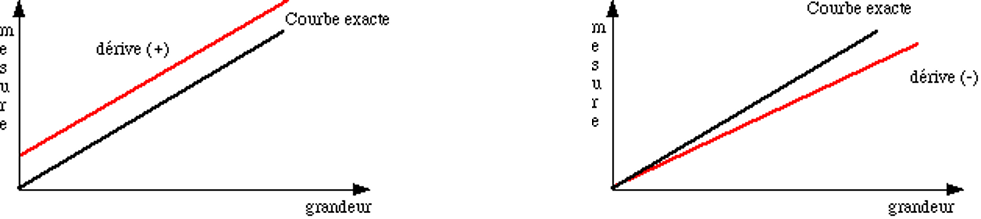
\includegraphics[width=\textwidth]{assets/figures/4_1_8_Erreurs_de_decalage_et_de_gain.PNG}
\caption{Erreurs de décalage et de gain}
\label{fig:Erreurs_de_decalage_et_de_gain}
\end{figure}

\begin{figure}[h!]
\centering
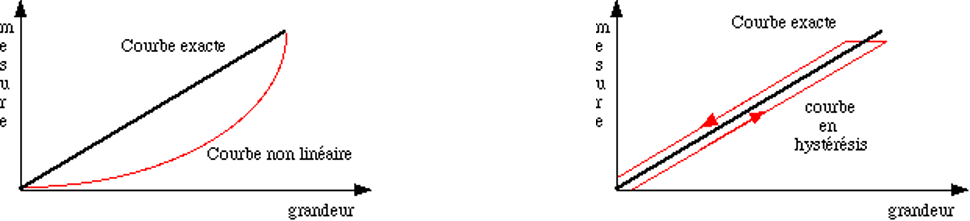
\includegraphics[width=\textwidth]{assets/figures/4_1_8_Erreurs_de_linearite_et_d_hysterese.PNG}
\caption{Erreurs de linéarité et d'hystérèse}
\label{fig:Erreurs_de_linearite_et_d_hysterese}
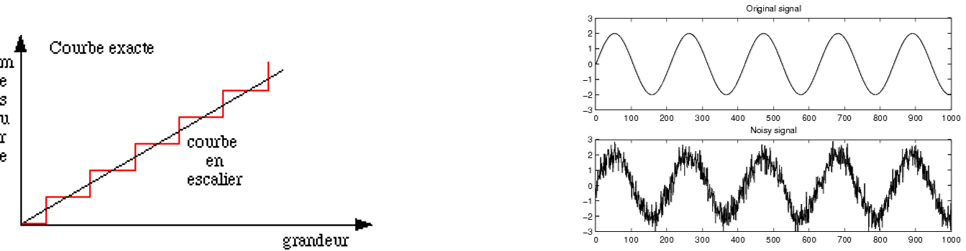
\includegraphics[width=\textwidth]{assets/figures/4_1_8_Erreurs_de_mobilite_et_bruit.PNG}
\caption{Erreurs de mobilité et bruit}
\label{fig:Erreurs_de_mobilite_et_bruit}
\end{figure}
Il faut en particulier différencier les erreurs systématiques et les erreurs aléatoires. L'erreur systématique est un décalage entre la valeur vraie et la valeur mesurée. L'erreur aléatoire peut se situer de part et d'autre de la valeur vraie.
\begin{figure}[h!]
\centering
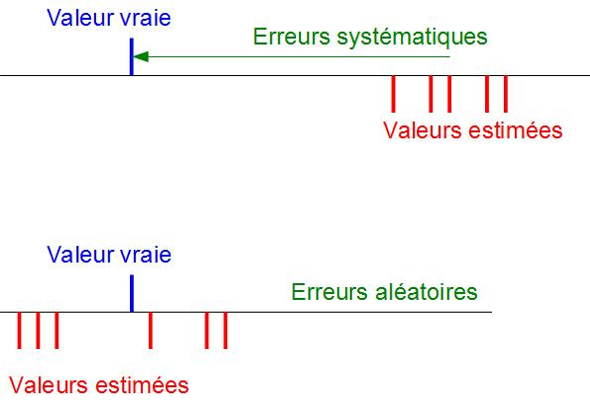
\includegraphics[height=6cm]{assets/figures/4_1_8_Erreurs_systematiques_et_aleatoires.PNG}
\caption{Erreurs systématiques et aléatoires}
\label{fig:Erreurs_systematiques_et_aleatoires}
\end{figure}
Les notions de justesse et de fidélité (ou répétabilité) sont associées à ces erreurs systématiques et aléatoires.

\section{Exemples de capteurs}

\subsection{Grandeurs électriques}

\subsubsection{Capteur de courant inductif}

Différent principaux permettent la mesure du courant électrique. Le transformateur de courant est une technique inductive basé sur un transformateur ayant au primaire une ou plusieurs spires avec le fil où la mesure de courant est effectuée. Au secondaire se trouve un ampèremètre. Le ratio entre le courant du secondaire et du primaire est proportionnel au rapport du nombre de spires entre le primaire et le secondaire.
\begin{figure}[h!]
\centering
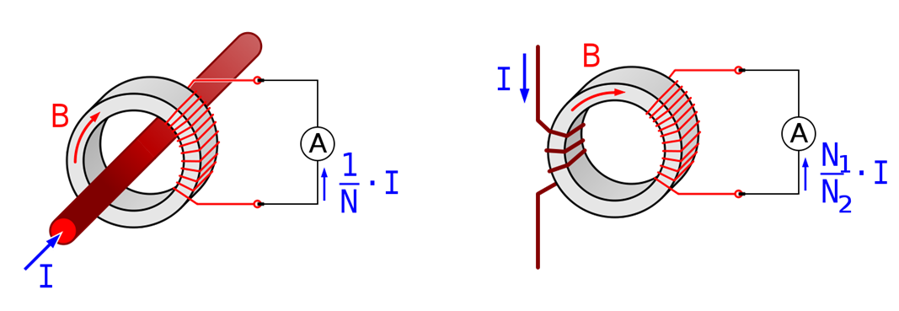
\includegraphics[height=5cm]{assets/figures/4_2_1_1_Capteur_de_courant_inductif.PNG}
\caption{Capteur de courant inductif (Source : Wikipedia).}
\label{fig:Capteur_de_courant_inductif}
\end{figure}

\subsubsection{Bobine de Rogowski}

La bobine de Rogowski est un cas particulier de mesure inductive sans entrefer. Il s'agit d'un solénoïde particulier placé autour du conducteur. La tension induite est peu/pas dépendante de la position du conducteur dans la boucle.

\begin{figure}[h!]
\centering
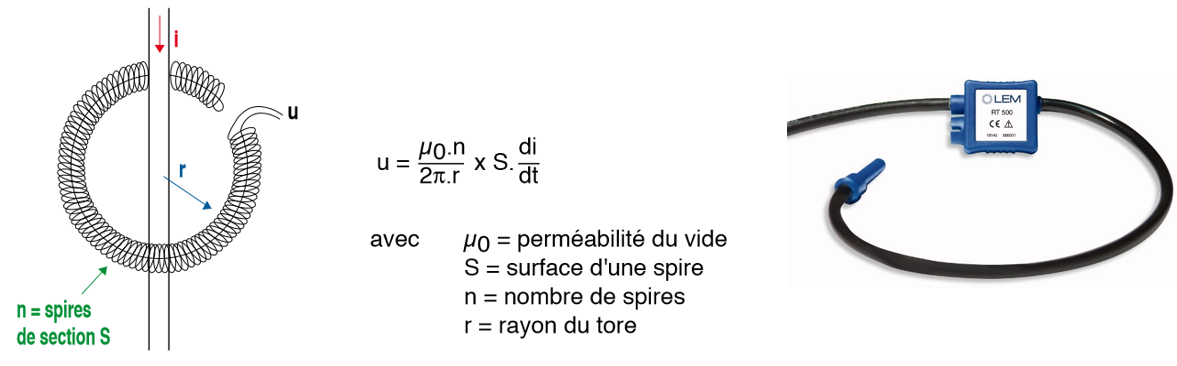
\includegraphics[width=15cm]{assets/figures/4_2_1_2_Bobine_de_Rogowski.PNG}
\caption{Bobine de Rogowski (Sources : Chauvin-Arnoux et LEM).}
\label{fig:Bobine_de_Rogowski}
\end{figure}


\subsubsection{Capteur de courant par effet Hall}
D'autres principes permettent de mesurer le courant, comme par exemple un capteur à effet Hall mesurant le champ magnétique autour du conducteur. Cette solution a comme gros avantage, par rapport aux techniques inductives, de permettre la mesure des courants continus.


\begin{figure}[h!]
\centering
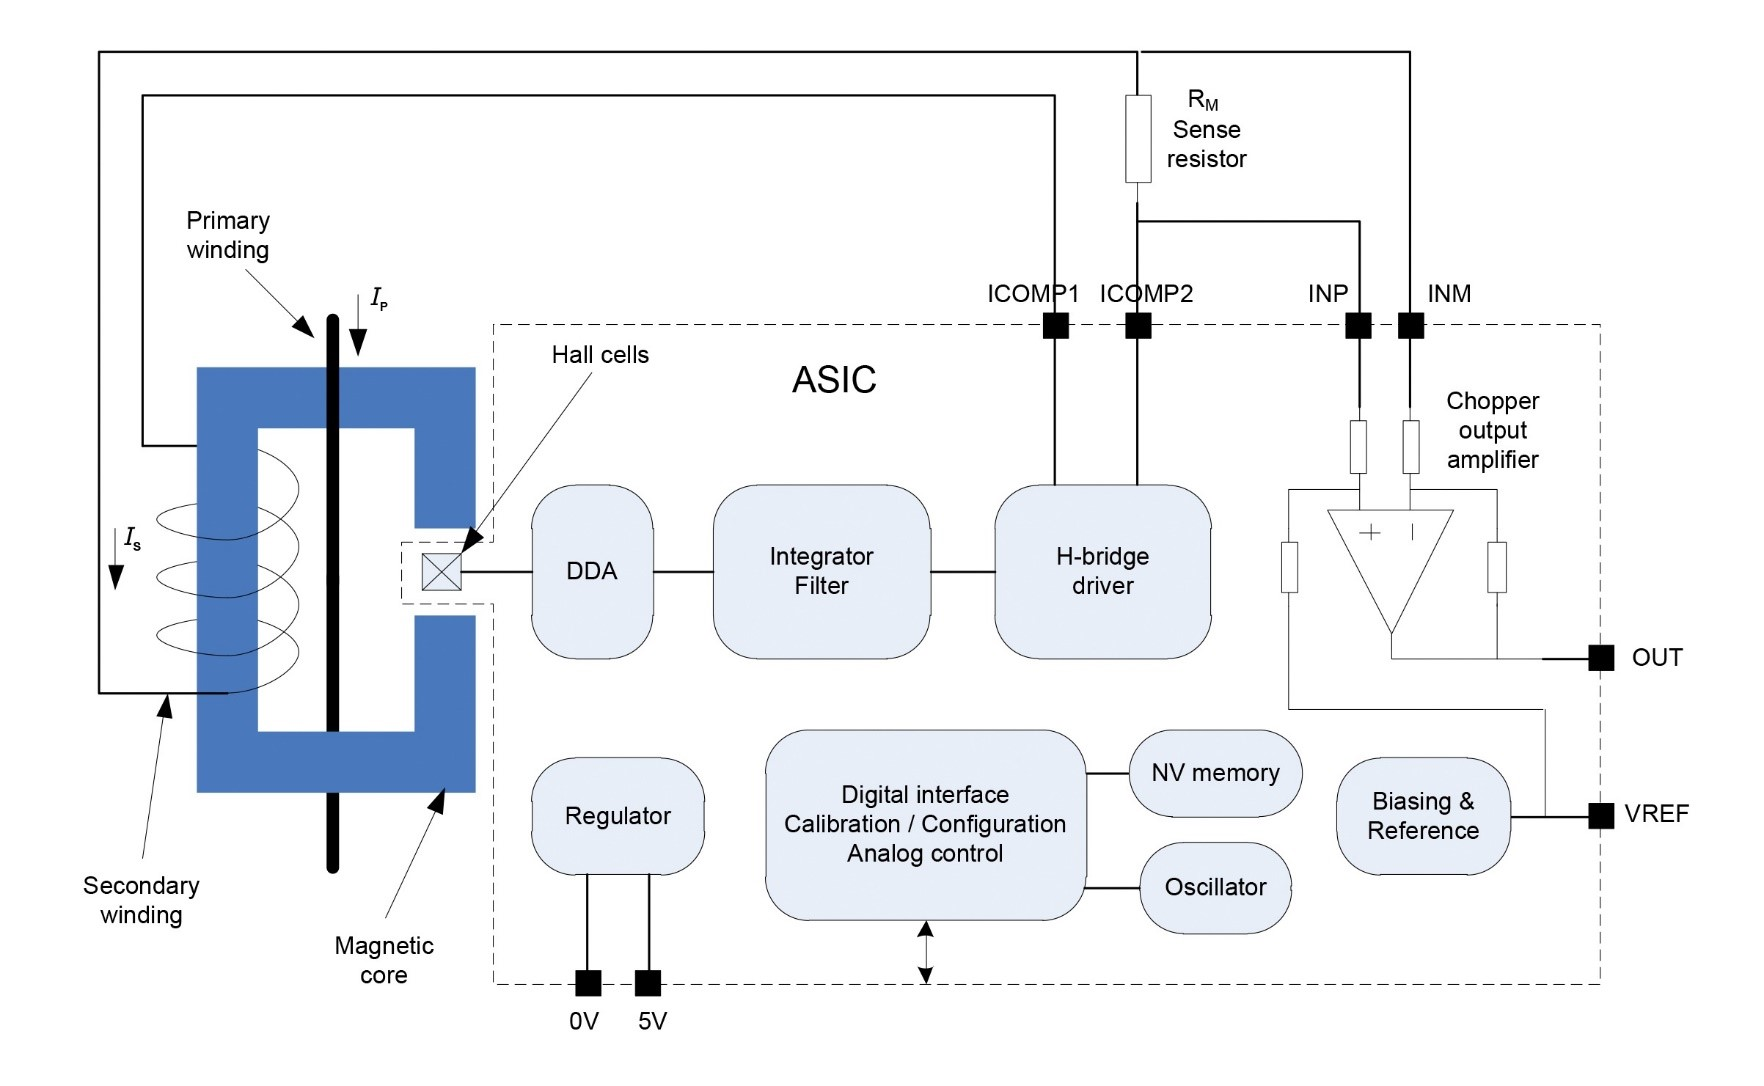
\includegraphics[width=15cm]{assets/figures/4_2_1_2_Capteur_de_courant_par_effet_Hall.jpg}
\caption{Capteur de courant par effet Hall (Source: LEM).}
\label{fig:Capteur_de_courant_par_effet_Hall}
\end{figure}

Ci-joint se trouve le schéma d'un capteur intelligent permettant la mesure en boucle fermée. Une contre-réaction permet de générer un champ magnétique s'opposant au champ magnétique lui-même généré par le courant à mesurer. Une structure à contre-réaction offre le grand avantage d'être sensible aux caractéristiques de la bobine plutôt qu'à la sensibilité du capteur à effet Hall.

\subsection{Température (TMP75 de Texas Instruments)}
Le TMP75 de Texas Instrument est un capteur intelligent disposant d'une interface I2C.

\begin{figure}[h!]
\centering
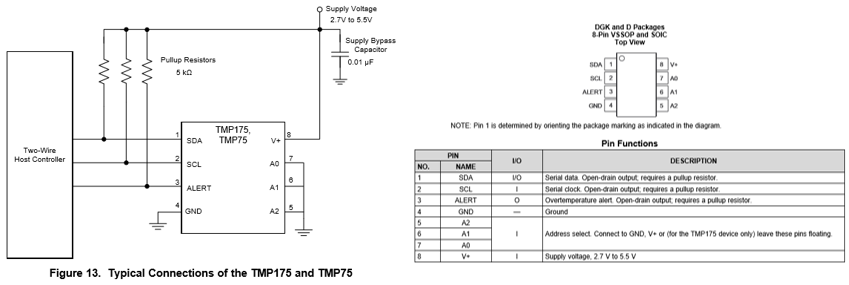
\includegraphics[width=15cm]{assets/figures/4_2_2_Temperature_TMP75.PNG}
\caption{Mesure de température avec le circuit TMP75}
\label{fig:Temperature_TMP75}
\end{figure}

Il se connecte aisément à un hôte, comme un microcontrôleur avec les deux signaux SDA et SCL. Une ligne supplémentaire ALERT permet en particulier de déclencher des interruptions.

Ce capteur intelligent dispose d'une cellule de mesure (Diode Temp. Sensor dans le schéma bloc ci-dessous), d'un convertisseur analogique numérique (convertisseur $ \Delta \Sigma$) et numérique-analogique.


\begin{figure}[h!]
\centering
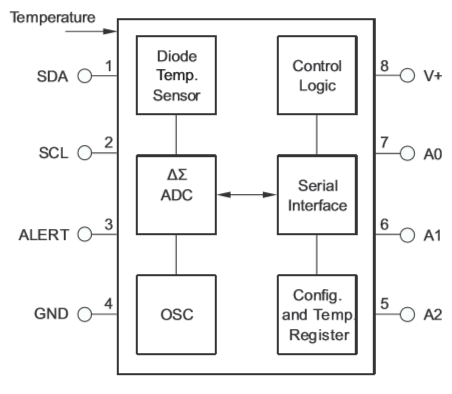
\includegraphics[height=6cm]{assets/figures/4_2_2_Temperature_TMP75_schema_bloc.PNG}
\caption{Schéma bloc circuit TMP75}
\label{fig:Temperature_TMP75_schema_bloc}
\end{figure}

Pour un capteur de température, la fiche technique donne un grand nombre de paramètres, comme en particulier les caractéristiques électriques ci-dessous. Chaque caractéristique peut avoir une grande importance pour une application.

\begin{figure}[h!]
\centering
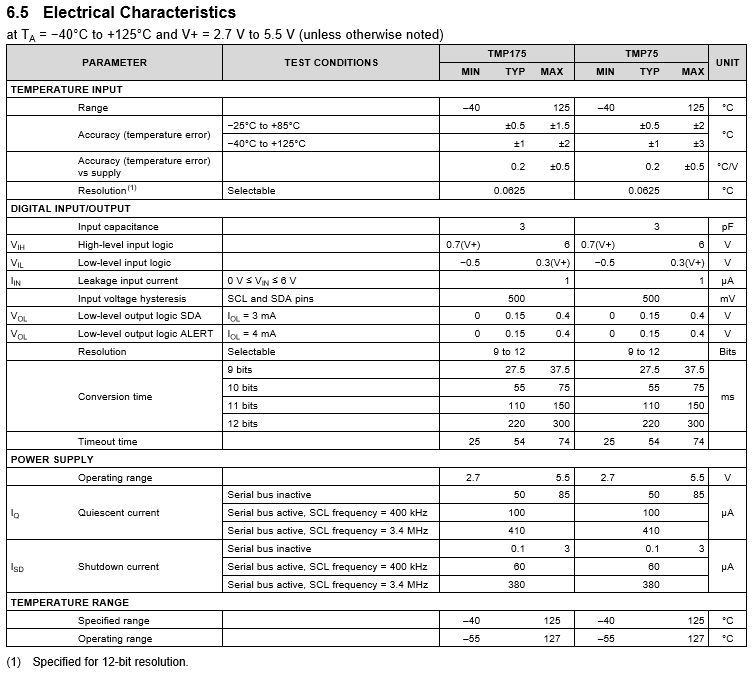
\includegraphics[width=15cm]{assets/figures/4_2_2_Temperature_TMP75_caracteristiques.PNG}
\caption{Caractéristiques du circuit TMP75}
\label{fig:Temperature_TMP75_caracteristiques}
\end{figure}



\subsection{Humidité (SHT3x-ARP de Sensirion)}
\begin{figure}[h!]
\centering
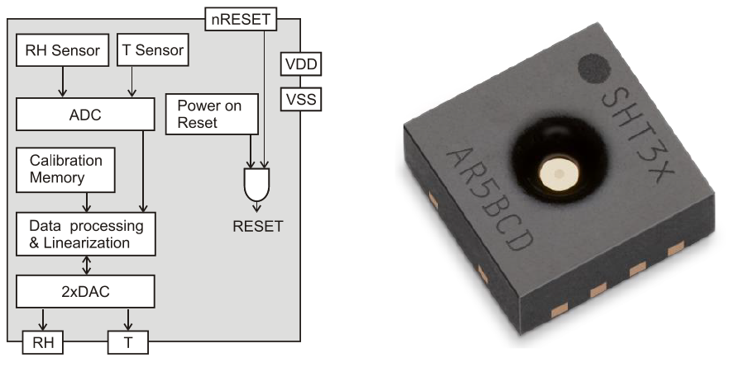
\includegraphics[width=8cm]{assets/figures/4_2_3_Humidite_SHT_3x_ARP.PNG}
\caption{Capteur d'humidité de Sensirion, SHT3x-ARP}
\label{fig:Humidite_SHT3x_ARP}
\end{figure}


La mesure de l'humidité avec ce capteur (Sensirion SHT3x-ARP) est une tension analogique radiométrique 10\% to 90\%. Cela veut dire que la mesure est proportionnelle à la tension d'alimentation. À noter un deuxième signal de température.


\begin{figure}[h!]
\centering
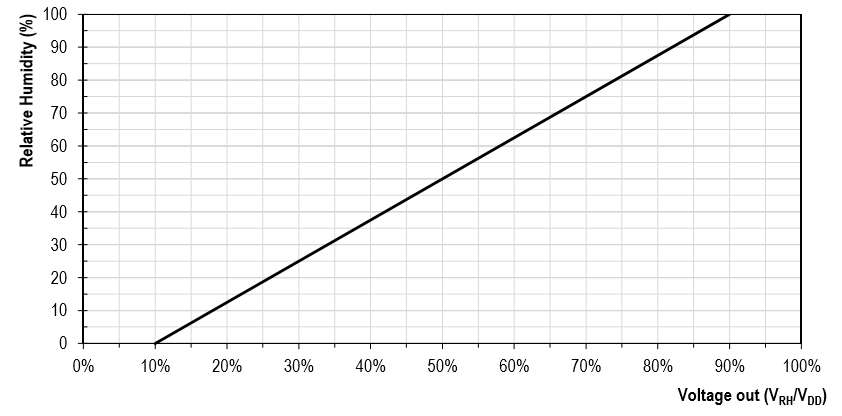
\includegraphics[width=15cm]{assets/figures/4_2_3_Humidite_SHT_3x_ARP_reponse.PNG}
\caption{Réponse du capteur d'humidité de Sensirion, SHT3x-ARP}
\label{fig:Humidite_SHT3x_ARP_reponse}
\end{figure}

L'incertitude de mesure se retrouve dans la fiche technique, avec une erreur typique et une erreur maximale.



\begin{figure}[h!]
\centering
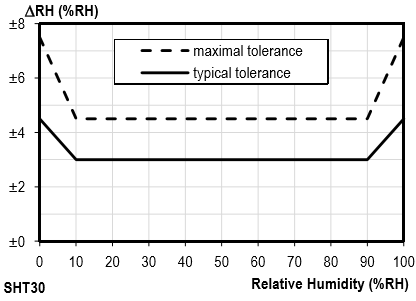
\includegraphics[width=10cm]{assets/figures/4_2_3_Humidite_SHT_3x_ARP_incertitude.PNG}
\caption{Incertitude de mesure du capteur d'humidité de Sensirion, SHT3x-ARP}
\label{fig:Humidite_SHT3x_ARP_incertitude}
\end{figure}

\subsection{Pression (Keller series 26 W)}
Le principe de fonctionnement de ce capteur de pression est une membrane se déformant sous l'effet de la différence de pression appliquée sur ces deux faces. Des piézorésistances (changement de résistance électrique d'un matériau dû à une contrainte mécanique) mesurent les contraintes mécaniques dans la membrane.


\begin{figure}[h!]
\centering
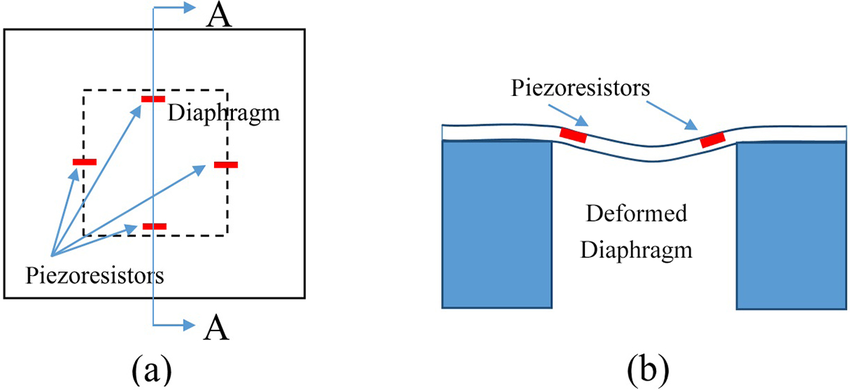
\includegraphics[width=10cm]{assets/figures/4_2_4_Pression_Keller_series26W.PNG}
\caption{Capteur de pression de Keller, series 26 W (Source : Kubba 2016)}
\label{fig:Pression_Keller_series26W}
\end{figure}

Ce capteur est utilisé pour mesurer des niveaux d'eau, indirectement en mesurant la pression due à la profondeur d'immersion. C'est la différence de pression avec la pression hors de l'eau qui est mesurée. Pour amener la pression atmosphérique au niveau de la membrane, un tuyau remonte en surface en passant dans le c‚ble (tube de ventilation).

\begin{figure}[h!]
\centering
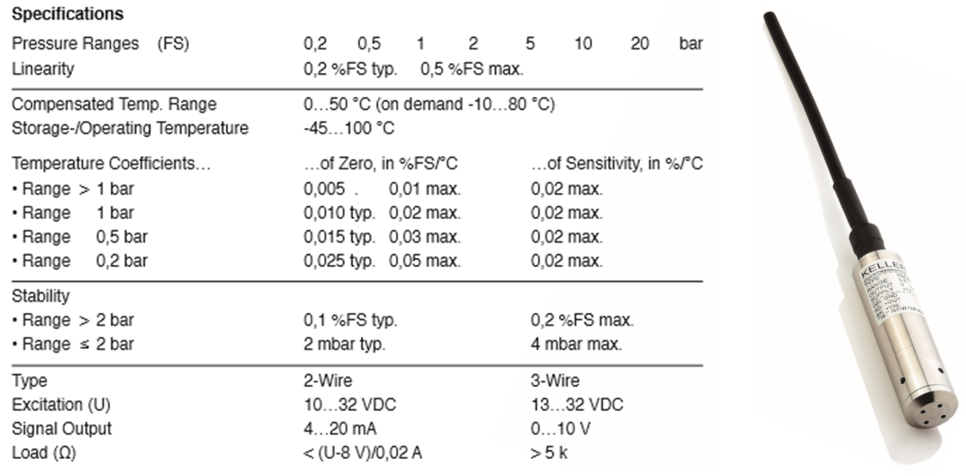
\includegraphics[width=15cm]{assets/figures/4_2_4_Pression_Keller_series26W_caracteristiques.PNG}
\caption{Caractéristiques du capteur de pression de Keller, series 26 W}
\label{fig:Pression_Keller_series26W_caracteristiques}
\end{figure}

\subsection{Jauges de déformation}
Dans une jauge, une déformation provoque une variation de la résistance. Cette variation de résistance répond à l'équation : \\
$\Delta R = k \ Delta L $
Avec :
$\Delta R$ : variation de résistance [$\Omega$]
$\Delta L$ : déformation [m]
k : coefficient ou facteur de jauge [$\Omega/m$]

\begin{figure}[h!]
\centering
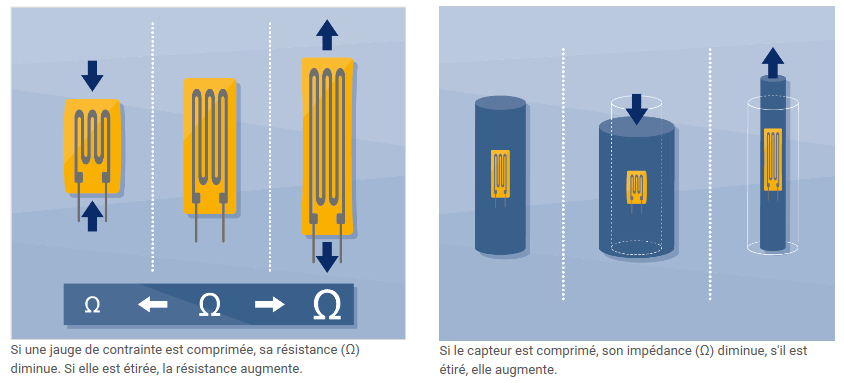
\includegraphics[width=15cm]{assets/figures/4_2_5_Jauges_de_deformation.png}
\caption{Jauges de déformation (source HBM)}
\label{fig:Jauges_de_deformation}
\end{figure}

Les jauges sont montées sur un corps d'épreuve. Les contraintes mécaniques entraînent une déformation. C'est cette déformation qui est mesurée par la jauge. Elle permet de retrouver la contrainte connaissant la rigidité du corps d'épreuve.


\subsection{Force (HBM RSCC)}

Les forces sont mesurées par la déformation d'un corps d'épreuve.
Pour ce capteur de force, des jauges de contraintes sont montées selon un pont de Wheastone sur les zones avec des contraintes mécaniques importantes et avec des paires où les contraintes mécaniques sont opposées (jauges 1-4 et 2-3).

\begin{figure}[h!]
\centering
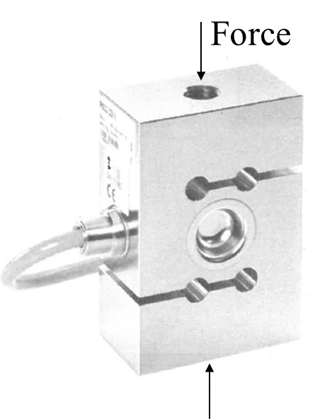
\includegraphics[width=7cm]{assets/figures/4_2_6_Force_HBM_RSCC.PNG}
\caption{Capteur de Force HBM RSCC (source HBM)}
\label{fig:Force_HBM_RSCC}
\end{figure}

\begin{figure}[h!]
\centering
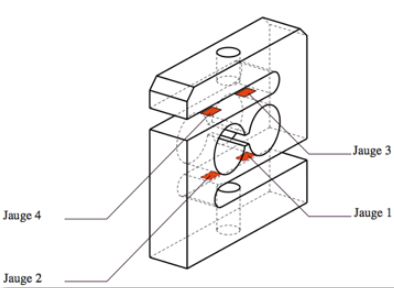
\includegraphics[width=7cm]{assets/figures/4_2_6_Force_HBM_RSCC_detail.PNG}
\caption{Capteur de Force HBM RSCC: détails}
\label{fig:Force_HBM_RSCC_detail}
\end{figure}

Le pont de Wheastone est composé de 4 résistances. Ces résistances sont remplacées par des jauges, avec une, deux ou quatre jauges, respectivement pour un quart de pont, demi-pont ou pont complet.
\begin{figure}[h!]
\centering
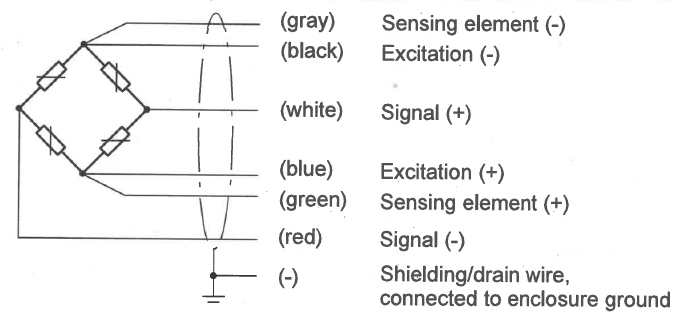
\includegraphics[width=7cm]{assets/figures/4_2_6_Force_HBM_RSCC_connexions.PNG}
\caption{Capteur de Force HBM RSCC: connexions}
\label{fig:Force_HBM_RSCC_connexions}
\end{figure}

\subsection{Couple (Omega TQ513)}
L'Omega TQ513 est un capteur de couple, basé sur des jauges de contraintes, placées sur une zone déformable (corps d'épreuve). Les jauges étant sur la partie tournante, un dispositif permet d'assurer le contact électrique glissant (slip rings).

\begin{figure}[h!]
\centering
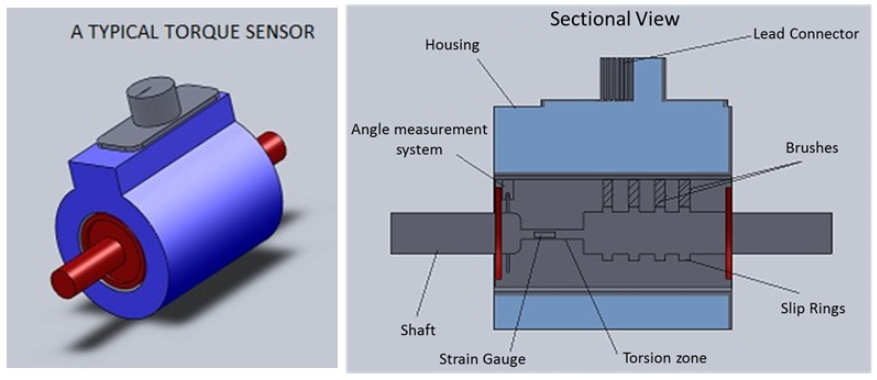
\includegraphics[width=7cm]{assets/figures/4_2_7_Couple_Omega_TQ513.PNG}
\caption{Capteur de couple: Omega TQ513}
\label{fig:Couple_Omega_TQ513}
\end{figure}

La déformation est liée aux propriétés mécaniques de la zone de torsion. Les jauges sont placées dans les axes de déformation maximale. Pour un pont complet, il y a une paire de jauge en compression et une paire en extension.


\begin{figure}[h!]
\centering
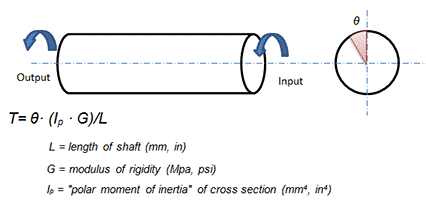
\includegraphics[width=7cm]{assets/figures/4_2_7_Couple_Omega_TQ513_principe.PNG}
\caption{Principe du capteur de couple (Source : https://cecas.clemson.edu)}
\label{fig:Couple_Omega_TQ513_principe}
\end{figure}

\subsection{Position linéaire (LT1300)}
Les capteurs LT1300 est un capteur de position linéaire, avec une gamme de 25 à 200mm.


\begin{figure}[h!]
\centering
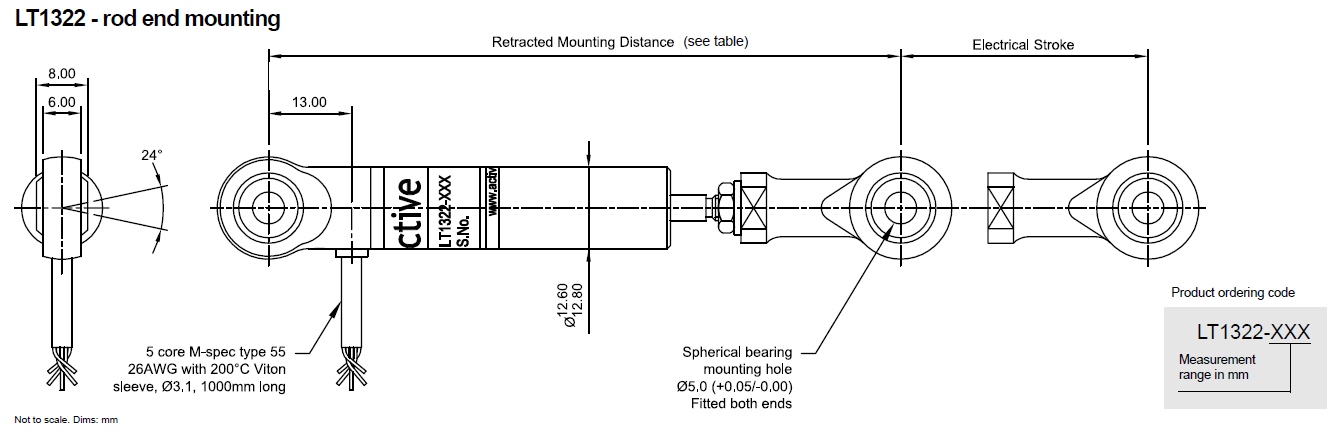
\includegraphics[width=7cm]{assets/figures/4_2_8_Position_lineaire_LT1300.PNG}
\caption{Capteur de position linéaire LT1300}
\label{fig:Position_lineaire_LT1300}
\end{figure}

Il fonctionne sur le principe du LVDT. C'est un principe inductif, utilisant un noyau ferromagnétique se déplaçant dans un transformateur pour modifier les couplages. Il utilise deux secondaires afin d'obtenir une réponse symétrique.

\begin{figure}[h!]
\centering
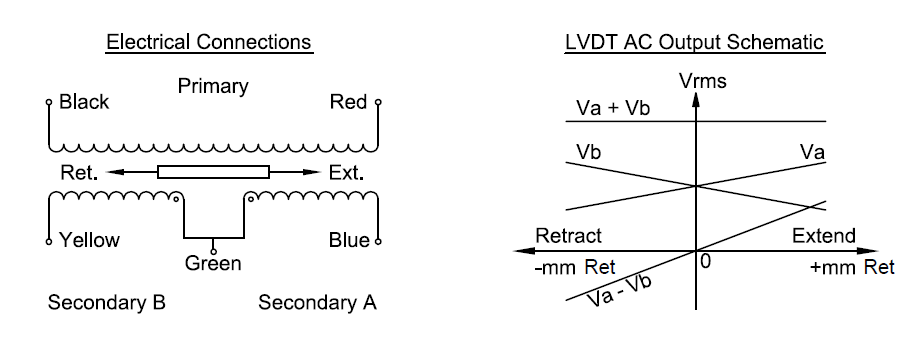
\includegraphics[width=7cm]{assets/figures/4_2_8_Position_lineaire_LT1300_detail.PNG}
\caption{Capteur de position linéaire LT1300: principe}
\label{fig:Position_lineaire_LT1300_detail}
\end{figure}

Un conditionneur de signal est nécessaire pour l'excitation du LVDT et pour effectuer la mesure. À noter que la réponse des LVDT n'est pas très linéaire, ce qui nécessite souvent une linéarisation.

\begin{figure}[h!]
\centering
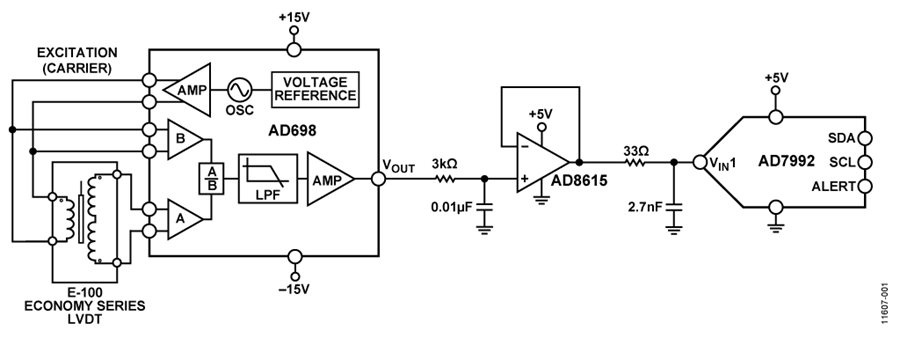
\includegraphics[width=7cm]{assets/figures/4_2_8_Position_lineaire_LT1300_conditionneur.PNG}
\caption{Capteur de position linéaire LT1300: conditionneur}
\label{fig:Position_lineaire_LT1300_conditionneur}
\end{figure}

\subsection{Position angulaire (Baumer GM400)}
Le Baumer GM400 est un codeur absolu. Il utilise un principe optique. Un disque codé avec des trous, tournant avec l'axe, permet de mesurer la position angulaire grâce à une source lumineuse est des photodétecteurs.

\begin{figure}[h!]
\centering
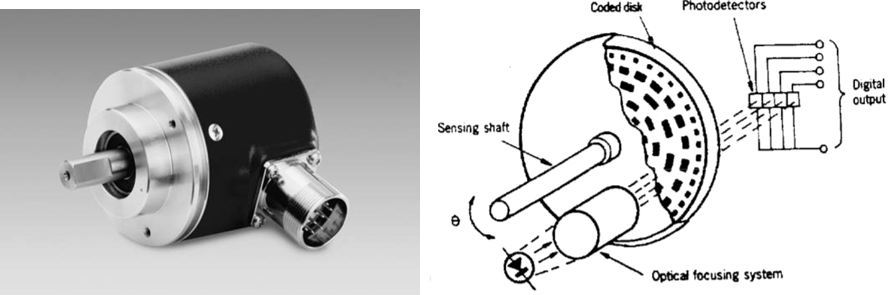
\includegraphics[width=7cm]{assets/figures/4_2_9_Position_angulaire_Baumer_GM400.PNG}
\caption{Position angulaire Baumer GM400 (Sources : Baumer et Guy Gauthier)}
\label{fig:Position_angulaire_Baumer_GM400}
\end{figure}

Pour certains codeurs optiques, le code binaire Gray est utilisé. Ce code offre l'avantage de ne modifier qu'un seul bit à la fois quand un nombre est augmenté d'une unité, contrairement au codage binaire naturel. Cela permet d'éviter des états transitoires lors des transitions.


\begin{figure}[h!]
\centering
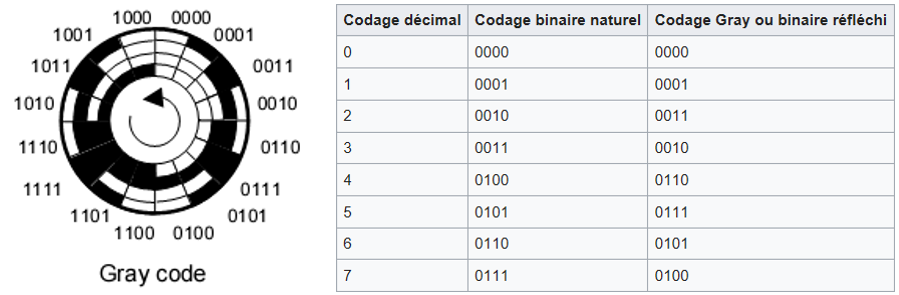
\includegraphics[width=7cm]{assets/figures/4_2_9_Position_angulaire_Baumer_GM400_codage.PNG}
\caption{Position angulaire Baumer GM400: codage}
\label{fig:Position_angulaire_Baumer_GM400_codage}
\end{figure}


Le transcodage binaire Gray/naturel est évidemment possible avec des algorithmes simples.

À noter que pour un capteur incrémental, deux signaux sont nécessaires pour connaître le sens de rotation. L'idée est d'utiliser deux signaux carrés déphasés de $90 \degree$.


\begin{figure}[h!]
\centering
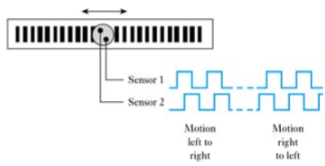
\includegraphics[width=7cm]{assets/figures/4_2_9_Position_angulaire_Baumer_GM400_fonctionnement.PNG}
\caption{Position angulaire Baumer GM400: fonctionnement}
\label{fig:Position_angulaire_Baumer_GM400_fonctionnement}
\end{figure}

\subsection{Vitesse (Philips KMI15/1)}
Le capteur de vitesse Philips KMI15/1 utilise un principe magnétique, avec une roue dentée ferromagnétique déformant le champ magnétique d'un aimant permanent.



\begin{figure}[h!]
\centering
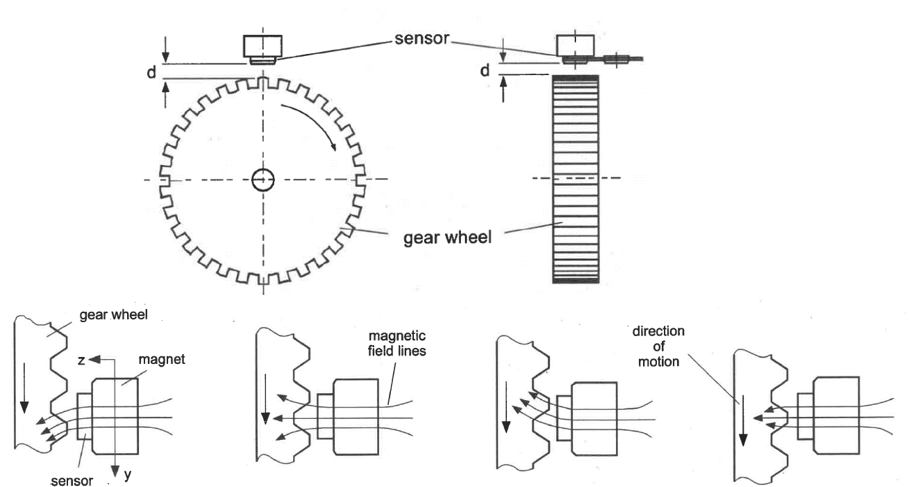
\includegraphics[width=7cm]{assets/figures/4_2_10_Vitesse_Philips_KMI15_1.PNG}
\caption{Capteur de vitesse: Philips KMI15/1}
\label{fig:Vitesse_Philips_KMI15_1}
\end{figure}

Le capteur KMI15/1 comprend l'aimant permanent et un capteur magnétorésitif (dont la résistance varie avec la magnétisation). La sortie du capteur est numérique de type tout ou rien (TOR).


\begin{figure}[h!]
\centering
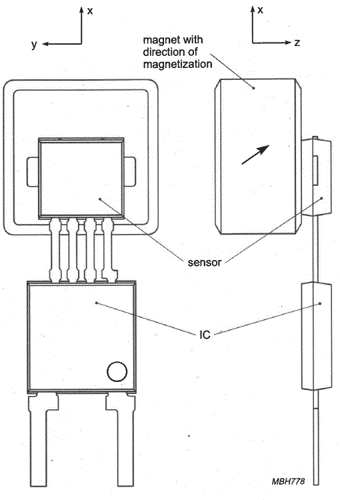
\includegraphics[width=7cm]{assets/figures/4_2_10_Vitesse_Philips_KMI15_1_detail.PNG}
\caption{Détail du capteur de vitesse Philips KMI15/1}
\label{fig:Vitesse_Philips_KMI15_1_detail}
\end{figure}

À noter encore que la mesure de vitesse avec une roue dentée est aussi possible en utilisant des capteurs de technologie inductive ou optique.


\subsection{Capteur de vibration (Colibrys VS1000)}

Le capteur de vibration Colibrys VS1000 est base sur une masse suspendue. Un principe capacitif permet de mesurer la position de la masse ou de créer des forces (pour le self-test)
Ce capteur dispose d'une sortie analogique radiométrique différentielle. Il dispose aussi d'une entrée pour lancer le self-test et d'un signal d'erreur en sortie. À noter encore la présence d'une mesure de température, souvent présente dans les capteurs intelligents.



\begin{figure}[h!]
\centering
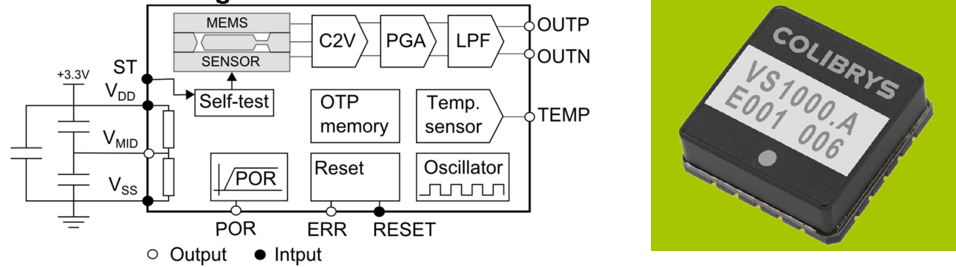
\includegraphics[width=7cm]{assets/figures/4_2_11_Capteur_de_vibration_Colibrys_VS1000.PNG}
\caption{Capteur de vibration: Colibrys VS1000}
\label{fig:Capteur_de_vibration_Colibrys_VS1000}
\end{figure}

\subsection{Capteur de proximité (Baumer CFDK 30N3600)}

Le capteur Baumer CFDK 30N3600 est un capteur de proximité capacitif. Il permet de détecter sans contact des objets métalliques et non métalliques à faible distance. Il permet aussi de détecter des niveaux de liquide à travers un réservoir. Un potentiomètre permet de régler la sensibilité du détecteur.

Ces capteurs de proximité disposent d'une sortie tout ou rien (TOR).

\subsection{Capteur chimique (Membrapor  CO/C-200)}

Les capteurs Membrapor  CO/C-200 sont des capteurs électrochimiques permettant la mesure de la concentration de monoxyde de carbone (CO). Pour ce type de capteurs, les dérives sont importantes, en particulier la dérive thermique, comme le montrent les graphiques ci-dessous.

\begin{figure}[h!]
\centering
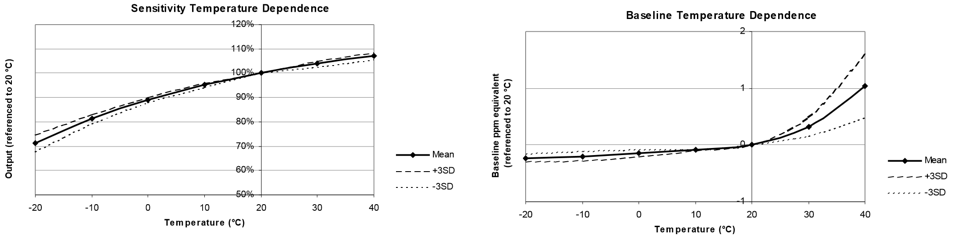
\includegraphics[width=7cm]{assets/figures/4_2_13_Capteur_chimique_Membrapor_CO_C_200.PNG}
\caption{Capteur chimique: Membrapor  CO/C-200}
\label{fig:Capteur_chimique_Membrapor_CO_C_200}
\end{figure}

À noter encore des grandeurs d'influence (cross-sensitivity) provenant d'autres gaz.

\begin{figure}[h!]
\centering
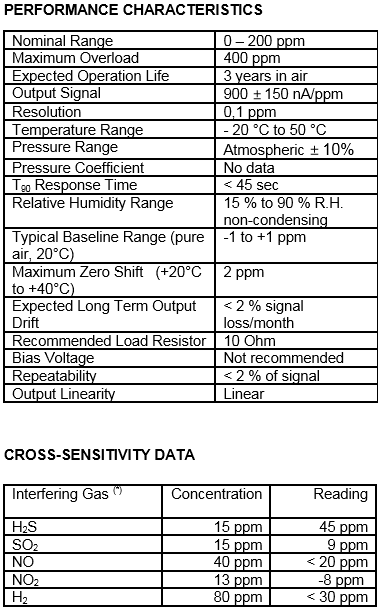
\includegraphics[width=7cm]{assets/figures/4_2_13_Capteur_chimique_Membrapor_CO_C_200_performance.PNG}
\caption{Capteur chimique Membrapor  CO/C-200: performances}
\label{fig:Capteur_chimique_Membrapor_CO_C_200_performance}
\end{figure}

\subsection{Capteur optique (Hamamatsu S-4251)}

Le capteur optique Hamamatsu S-4251 est constitué d'un driver pour une led exerne, une photodiode (c'est la raison du boîtier transparent) et une électronique de mesure utilisant le principe de la détection synchrone.

\begin{figure}[h!]
\centering
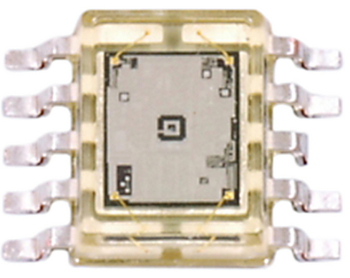
\includegraphics[width=7cm]{assets/figures/4_2_14_Capteur_optique_Hamamatsu_S_4251.PNG}
\caption{Capteur optique:Hamamatsu S-4251}
\label{fig:Capteur_optique_Hamamatsu_S_4251}
\end{figure}

Il y a souvent dans les capteurs des composantes de bruit à basses fréquences (bruit 1/f ou de la dérive). Il y a aussi souvent la présence de perturbations à basse fréquence. Par exemple des variations lentes de la lumière ambiante ou un scintillement à 50Hz. Le principe de la détection synchrone consiste à moduler le signal à mesurer pour se retrouver avec une fréquence plus élevée que ces bruits à basse fréquence.

\begin{figure}[h!]
\centering
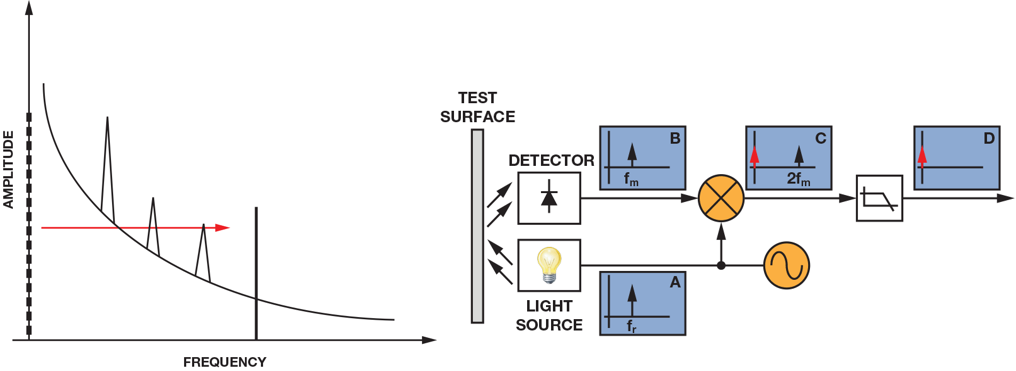
\includegraphics[width=7cm]{assets/figures/4_2_14_Capteur_optique_Hamamatsu_S_4251_conditionneur.PNG}
\caption{Capteur optique Hamamatsu S-4251: exemple de conditionneur (source: Analog Devices)}
\label{fig:Capteur_optique_Hamamatsu_S_4251_conditionneur}
\end{figure}

Dans ce capteur, le principe consiste à moduler la lumière vers 10kHz. Le signal reçu est alors démodulé en phase. Cela permet de s'affranchir de toutes les composantes de bruit à plus basse fréquence.

\subsection{Lectures conseillées}

\begin{itemize}
\item " Les capteurs en instrumentation industrielle ", Georges Asch et Bernard Poussery, Dunod, 2017.
\item " Acquisition de données, du capteur à l'ordinateur ", Gorge Asch, Dunod, 2011.
\end{itemize}

%\end{document}

    \chapter{La mesure et sa représentation}
\label{chap:measurements}

Lors de tout procédé expérimental, on effectue des mesures. Une mesure brute, seule, ne veut presque rien dire (éventuellement on obtient l'ordre de grandeur). Il faut lui adjoindre une estimation d'incertitude. La plupart du temps, lorsque l'on a besoin d'une connaissance précise des caractéristiques d'un système quelconque, on va réaliser un grand nombre de mesures individuelles de ces propriétés, et c'est l'analyse statistique des mesures qui va nous permettre d'estimer les propriétés du système, avec marge d'incertitude. Cette démarche en deux temps, (1) acquisition d'un nombre significatif de données (2) traitement statistique de ces données, constitue le c\oe ur de la démarche expérimentale. Elle seule permet d'obtenir des résultats valides.

Avant d'appliquer les outils de l'analyse statistique à un échantillon de mesures, il est cependant indispensable d'examiner \textbf{la qualité de l'échantillon}: existe-t-il des valeurs aberrantes qu'il faudrait rejeter ? Y a-t-il assez de mesures ? etc. On utilise pour cela des outils de représentation simples: moyenne, écart-type, et surtout, l'histogramme. Ce chapitre est donc dédié à la définition de ce que c'est qu'une mesure, et des outils permettant de la valider, et de la caractériser.

\section{Définitions}

\subsection{L'échantillon}

Soit une grandeur physique $\mathcal{G}$ (par exemple une tension électrique) et un ensemble de $N_m$ mesures de $\mathcal{G}$. Cet ensemble est appelé un \textbf{échantillon} $\mathcal{E}$ de $\mathcal{G}$. Quelques exemples:
\begin{description}
\item[mesures de la tension aux bornes d'une résistance] $\mathcal{E}=[3.5,3.4,3.1,3.7]$ mV,
\item[cinq jets d'un dé à 6 faces] $\mathcal{E}=[5,4,1,2,2]$,
\item[une séquence du génome humain] $\mathcal{E}=[A,G,G,T,A,G,G,T,C,C,A]$,
\item[mesure d'un diamètre d'axe] $\mathcal{E}=[19.998,20.004,20.003,19.997,20.013]$ mm.
\end{description}
On voit que les éléments d'un échantillon peuvent être de tout type, entier ou réel, et même non numérique. Ce qui caractérise un échantillon, c'est la \textbf{nature} et le \textbf{nombre} de ses éléments (quoi, et combien).

\subsection{La population}

La population $\mathcal{P}$ d'une grandeur $\mathcal{G}$ est définie par \textbf{l'ensemble de toutes les valeurs possibles que peut prendre cette grandeur}. C'est à partir de la population que l'on forme des échantillons. Quelques exemples:
\begin{description}
\item[dé à 6 faces] $\mathcal{P}=[1,2,3,4,5,6]$,
\item[les lettres du génome humain] $\mathcal{P}=[A,C,G,T]$
\item[mesure d'un diamètre de 20 mm] $\mathcal{P}=\infty$ !
\end{description}
Quelques remarques s'imposent:
\begin{itemize}
\item la longueur d'un échantillon peut être inférieure, égale ou supérieure à la dimension de la population: il s'agit simplement du nombre de mesures effectuées;
\item la dimension d'une population peut être infinie ! par exemple, dans le cas de la mesure du diamètre d'un axe, les fluctuations de la mesure dues à la précision toujours limitée de l'instrument de mesure, ou aux variations de la pièce elle-même (dilatation/contraction thermique), vont induire une mesure dont la différence avec la valeur réelle sera aléatoire.
\end{itemize}
Il n'est pas toujours évident de déterminer la population d'une mesure. Seule une inspection détaillée du processus de mesure nous permettra de déterminer au cas par cas la population complète de $\mathcal{G}$.

À quoi sert-il de déterminer la population ? Tout simplement à connaître à l'avance les résultats possibles des mesures, et éliminer par avance les mesures impossibles. Un exemple: admettons qu'un ingénieur ait mis au point un appareil automatique de mesure de diamètre, et que l'on soumette à cet appareil un axe cylindrique de 20 mm de diamètre. Quatre mesures sont effectuées, et l'échantillon est le suivant $\mathcal{E}=[19.9,20.1,1.7,19.8]$ mm. Immédiatement, on voit que la valeur des 3$^\text{ème}$ mesures n'a aucun sens, elle ne peut vraiment pas faire partie de la population. L'ingénieur en conclut qu'il y a un problème avec le procédé de mesure.

\subsection{L'analyse statistique}

L'analyse statistique \textit{est un ensemble de méthodes de traitement numérique d'un échantillon permettant d'estimer les propriétés de la population dont il est issu.}

Pour donner un exemple, imaginons que nous disposions d'un échantillon de mesure d'une tension électrique. Les outils de l'analyse statistique nous permettront de calculer l'incertitude sur la moyenne de l'échantillon, ce qui est une information aussi importante que la moyenne elle-même.

On peut aussi dire: \textit{l'analyse statistique permet de réduire un ensemble de données brutes en un petit nombre de valeurs caractéristiques de la population associée}. C'est assez identique à la première définition. On parle aussi de \textbf{réduction} des données.

\section{Moyenne, écart quadratique moyen, écart-type}

Soit un échantillon de $N_m$ mesures de la grandeur $\mathcal{G}$. Désignons par $x_i$ la valeur de la mesure individuelle numéro $i$, avec $i=1\dots N_m$.

\subsection{La moyenne de l'échantillon}

Elle est définie par
\begin{equation}
\langle x\rangle=\frac{1}{N_m}\sum\limits_{i=1}^{N_m}\,x_i
\end{equation}
Notation: les parenthèses angulaires $\langle\cdot\rangle$ désignent l'opération de moyenne. On rencontre aussi dans la littérature le symbole $\overline{x}$, mais la première notation est plus fréquente.

\subsection{L'écart quadratique moyen de l'échantillon}

C'est la moyenne de l'écart quadratique (c.-à-d. au carré) entre les éléments de l'échantillon et sa valeur moyenne $\langle x\rangle$,
\begin{equation}
\text{EQM}(x)=\langle (x-\langle x\rangle)^2\rangle
\end{equation}
Si nous développons, il vient
$$
\langle (x-\langle x\rangle)^2\rangle=\langle x^2-2x\langle x\rangle+\langle x\rangle^2\rangle
=\langle x^2\rangle-2\langle x\rangle\langle x\rangle+\langle\langle x\rangle^2\rangle
=\langle x^2\rangle-2\langle x\rangle^2+\langle x\rangle^2
=\langle x^2\rangle-\langle x\rangle^2
$$
d'où, en appliquant la définition de la moyenne
\begin{equation}
\text{EQM}(x)=\frac{1}{N_m}\sum\limits_{i=1}^{N_m}\,x_i^2-
\left(\frac{1}{N_m}\sum\limits_{i=1}^{N_m}\,x_i\right)^2
\end{equation}
À noter que l'on désigne aussi l'écart quadratique moyen par la \textbf{variance} de l'échantillon, mais comme ce dernier terme possède une définition très spécifique en relation avec les distributions de probabilité, il vaut mieux ne pas l'utiliser dans le contexte d'un échantillon de taille finie.

\subsection{L'écart-type de l'échantillon}

Il est simplement défini par la racine carrée de l'écart quadratique moyen, et on le note avec le symbole $\sigma$
\begin{equation}
\sigma(x)=\sqrt{\text{EQM}(x)}
\end{equation}
Il représente la \textbf{dispersion typique des mesures} autour de la moyenne.
\vspace{3mm}
\begin{center}
\fbox{
\begin{minipage}{12cm}\textbf{L'écart-type et la moyenne constituent les deux outils centraux de l'analyse statistique d'un échantillon.}
\end{minipage}
}
\end{center}

\section{La représentation d'un échantillon de mesures à l'aide d'un histogramme}

\begin{figure}[htb]
   \centering
   \vspace{-5mm}
   \includegraphics[width=6cm]{assets/figures/serie1000points.pdf} \hspace{5mm}
   \includegraphics[width=6cm]{assets/figures/serie1000points_histogram.pdf}
   \caption{\it À gauche: les 1000 premières mesures d'une série de 100'000 mesures, pour lesquelles on sait qu'il existe une mesure parasite autour de la valeur 1. Elle est invisible dans ce graphique. À droite: histogramme des 100'000 mesures. En noir, histogramme sans le signal parasite. En rouge, histogramme avec le signal parasite.}
   \label{fig:sdp}
\end{figure}
En général, les échantillons de mesure sont constitués d'un grand nombre d'éléments - quelques dizaines lorsque l'acquisition se fait à la main, à plusieurs milliers ou plus lorsque l'acquisition se fait de manière automatique (ce qui est préférable).

Or, avant d'exploiter les données, il faut les examiner, afin de détecter un problème éventuel - ce qui arrive toujours lors de la phase de mise au point d'un instrument ou d'une machine. Il est donc crucial de \textbf{visualiser} les échantillons. Si la dimension de l'échantillon est grand, il peut être pratiquement impossible (ou peu pratique) d'examiner chaque mesure individuelle (figure~\ref{fig:sdp}). Dans ce cas, on utilisera avec avantage une représentation graphique, \textbf{l'histogramme}.

L'idée de l'histogramme consiste à segmenter l'intervalle entre la valeur minimale et la valeur maximale de l'échantillon en $N_c$ sous-intervalles - ou classes - de même largeur, puis à compter le nombre de fois que les mesures tombent dans chacune des classes. On établit alors un graphique montrant le nombre de mesures dans chaque classe, qui nous donne une vue d'ensemble immédiate, permettant de détecter la présence éventuelle de mesures problématiques, pour autant que nous ayons une idée préalable des valeurs que peuvent prendre les mesures (la population).

Considérons l'exemple de la figure~\ref{fig:sdp}. Il s'agit d'un échantillon de 100'000 mesures d'une grandeur physique (quelconque, dont on ne précise pas l'unité) de moyenne nulle, et d'écart-type $\sigma=1$. On montre la série des 1'000 premiers points de mesure. On a ajouté, à cette série de mesures, un \textbf{signal parasite} de moyenne égale à 1 et d'écart-type 0.1. Ce signal parasite n'est pas du tout visible parmi la série des 1'000 points de mesure. En revanche, l'histogramme montre très bien, centré sur 1, un excès du nombre de mesures (ou fréquence) par rapport à la fréquence des valeurs voisines.

\begin{figure}[h]
   \centering
   \includegraphics[height=6cm]{assets/figures/serie1000points_histogram_20classes.pdf} \hspace{5mm}
   \includegraphics[height=6cm]{assets/figures/serie1000points_histogram_2000classes.pdf}
   \caption{Histogramme des 100'000 mesures, avec 20 classes, à gauche, et 2000 classes, à droite. En noir, histogramme du signal sans signal parasite. En rouge, histogramme du signal avec le signal parasite.}
   \label{fig:hapoabdc}
\end{figure}
Toute la difficulté consiste à choisir le nombre de classes. Dans l'exemple ci-dessus, nous avons considéré 200 classes. Si nous avions pris moins de classes, par exemple 20, alors l'histogramme serait plus lisse (figure~\ref{fig:hapoabdc}), mais la résolution trop grossière, et nous n'aurions pas détecté les mesures parasites. En revanche, avec beaucoup de classes (2000), la résolution est grande, mais l'histogramme devient plus chaotique, et il se pourrait que le signal parasite soit noyé dans les fluctuations statistiques (ce qui n'est en fait pas encore le cas ici).

Une bonne méthode empirique pour choisir le nombre de classes est de prendre la racine carrée du nombre de mesures. Pour 100'000, nous devrions prendre 316 classes. Quoi qu'il en soit, le nombre optimal de classes sera celui qui nous permettra de visualiser au mieux les propriétés de notre échantillon de mesures. On a vu que pour notre exemple, avec 200 classes on obtient en pratique une très bonne représentation.

\subsection{Comment interpréter un histogramme ?}

\begin{itemize}
\item si l'histogramme est symétrique, alors la valeur sur laquelle il est centré est une indication de la valeur moyenne de l'échantillon; s'il n'est pas symétrique, on ne peut rien dire sur la valeur moyenne, et il faut faire un calcul;
\item la valeur de la mesure correspondant au maximum de l'histogramme définit le \textbf{mode} de l'échantillon. C'est la valeur \textbf{la plus fréquente}. Qui se confond avec la valeur moyenne seulement si l'histogramme est symétrique;
\item la largeur à mi-hauteur de l'histogramme est une indication de la dispersion des mesures, et est directement reliée à l'écart-type $\sigma(x)$.
\item la forme de l'histogramme est une indication du type de processus statistique à l'\oe uvre lors de l'acquisition de l'échantillon (on aura des processus de type gaussien, poissonien, binomial, uniforme, etc - que l'on introduira plus loin). Or, il est possible de prévoir, pour un processus de mesure donné, le type de distribution attendu. La comparaison de la forme de l'histogramme des mesures avec la distribution prévue nous permettra de confirmer que le système se comporte de la manière attendue. Par exemple, le pic dans l'histogramme de l'exemple précédent dévoile l'existence du signal parasite, car en général, toutes les mesures de grandeurs physiques suivent des distributions régulières (ici une distribution dite gaussienne).
\end{itemize}

\subsection{La distribution gaussienne}

On discutera, dans le chapitre dédié aux distributions, de la répartition dite gaussienne d'une mesure aléatoire. Mais comme il s'agit d'une distribution très fréquemment utilisée en pratique, et que nous utilisons souvent comme référence, il est utile de l'introduire rapidement ici.

Dans la grande majorité des cas, lorsque l'on mesure la valeur d'une grandeur physique de type \textbf{réel}\footnote{c.-à-d. ne prenant pas des valeurs discrètes, mais pouvant avoir toute valeur dans l'intervalle des nombres réels} soumise à des fluctuations aléatoires, comme la tension électrique, la température, etc., on trouve que les mesures se répartissent symétriquement autour d'une moyenne, selon une courbe dite \textit{en cloche}. L'équation de cette répartition est la suivante
\begin{equation}
g(x)=\frac{1}{\sigma\sqrt{2\pi}}\exp{\left[-\frac{(x-\mu)^2}{2\sigma^2}\right]}
\end{equation}
ou $\mu$ représente la moyenne des mesures et $\sigma$ l'écart-type de la grandeur physique $x$. Les 100'000 points dont on a représenté l'histogramme à 20 classes en figure~\ref{fig:hapoabdc} suit une distribution gaussienne de moyenne $\mu=0$ et d'écart-type $\sigma=1$.

\subsection*{Histogramme, ou distribution de probabilité ? et combien de mesures faut-il acquérir ?}

Il y a une grande différence conceptuelle entre un histogramme et une distribution de probabilité. Un histogramme n'est qu'une représentation graphique des fréquences associées à \textbf{un seul échantillon} de mesures. En principe, si on enregistre N échantillons de mesures de la même grandeur physique, on va tomber sur N histogrammes légèrement différents les uns des autres car il n'y a aucune raison de mesurer à chaque fois la même série de valeurs !

En revanche, si on effectue une infinité de mesures ($N_m\rightarrow\infty$), alors la fréquence relative $p_k=f_k/N_m$ va tendre vers une valeur stable, constante, qui pourra s'interpréter comme la probabilité que la mesure tombe dans la classe $k$. On verra alors plus loin que dans ce cas, il peut y avoir égalité exacte entre les moyennes et EQM calculés à partir de l'échantillon ou à partir de la distribution des probabilités.

Il ressort de tout cela que si on désire avoir une bonne estimation de la structure de la distribution des valeurs, il faut considérer des échantillons de mesure assez grands.  Typiquement, une centaine de mesures permet déjà de se faire une idée de la répartition sous-jacente. Mais ce n'est qu'avec 1000 points que l'on arrive vraiment à identifier le type de distribution. La figure~\ref{fig:h123} montre l'évolution de l'histogramme associé à une \begin{wrapfigure}[19]{l}[0pt]{6cm}
   \centering
   \includegraphics[width=6cm]{assets/figures/histGaussienDixCentMilleMesures.pdf}
   \caption{\it Histogramme d'une mesure gaussienne de moyenne nulle et d'écart-type 1, pour des échantillons de 10, 100 et 1000 mesures.}
   \label{fig:h123}
\end{wrapfigure}
distribution gaussienne, lorsque l'on considère 10, 100 et 1000 points de mesure. On voit qu'avec 10 points (et donc 3 classes), il est impossible de dire quoi que ce soit. Avec 100 points (courbe bleue, 10 classes) on commence à voir que la distribution est centrée, compacte, avec un maximum autour de 0. Avec 1000 points (30 classes), la distribution gaussienne devient évidente.

On peut montrer, en théorie statistique, que si on dispose de $N_m$ mesures d'une grandeur physique quelconque $G$, alors l'erreur commise sur la détermination de la vraie moyenne est égale à l'écart-type de l'échantillon divisé par la racine carrée de $N_m$,
\begin{equation}
\text{err}(\langle G\rangle)=\frac{\sigma_G}{\sqrt{N_m}}
\end{equation}
Par conséquent, l'erreur relative due au nombre fini de mesures va comme $1/\sqrt{N_m}$. Par conséquent, si on veut une précision de 1\% sur la moyenne, il faudra acquérir au moins 10'000 mesures. Cette règle fonctionne très bien, pour tout type de mesure.

\section{Histogramme cumulé}

Un autre outil de représentation pratique de l'échantillon est constitué par le cumul des fréquences, c.-à-d. la détermination du nombre de fois $F_k$ que la mesure x est comprise dans une classe donnée ou dans les classes précédentes,
$$
F_k=\text{nombre de fois que x $\in$ classes } 1,2,\cdots,k
$$
c.-à-d.
\begin{equation}
F_k=\sum\limits_{i=1}^{k}\,f_k
\end{equation}
\begin{wraptable}[6]{r}[0pt]{44mm}
\centering
\vspace{-6mm}
\begin{tabular}{cccccc}
 8 &  1 &  2 &  1 &  2 &  7 \\
 5 & 10 &  1 &  9 &  4 &  6 \\
10 &  9 &  5 &  4 &  2 &  3 \\
 5 &  2 &  0 &  1 &  5 &  4 \\
 4 &  6 &  6 &  7 &  4 &  5 \\
 6 &  4 & 10 &  3 &  0 &  4
\end{tabular}
\end{wraptable}
Considérons par exemple un échantillon de 36 éléments (ci-contre), tiré d'une distribution uniforme. La moyenne de l'échantillon est 4.72 et l'écart-type 3.00. Considérons 5 classes, et calculons les fréquences de chaque classe. La largeur des classes sera donnée par $\Delta x=(\text{max}(x)-\text{min}(x))/N_c=10/5=2$. On trouve
\begin{center}
\begin{tabular}{cccc}
classe $k$ & intervalle & val. centrale $x_k$ & fréquence $f_k$ \\\hline
1 & [0,2[ & 1 & 6 \\
2 & [2,4[ & 3 & 6 \\
3 & [4,6[ & 5 & 11 \\
4 & [6,8[ & 7 & 6 \\
5 & [8,10] & 9 & 7 \\\hline
\end{tabular}
\end{center}
L'histogramme correspondant est montré en Fig.~\ref{fig:hcapoabdc}, gauche. Les fréquences cumulées sont données ci-dessous, et l'histogramme cumulé correspondant en Fig.~\ref{fig:hcapoabdc}, droite.
\begin{center}
\begin{tabular}{ccccc}
classe $k$ & intervalle & val. centrale $x_k$ & fréquence $f_k$ & fréq. cum. $F_k$\\\hline
1 & [0,2[ & 1 & 6 & 6 \\
2 & [2,4[ & 3 & 6 & 12 \\
3 & [4,6[ & 5 & 11 & 23 \\
4 & [6,8[ & 7 & 6 & 29 \\
5 & [8,10] & 9 & 7 & 36\\\hline
\end{tabular}
\end{center}
\begin{figure}[h]
   \centering
   \includegraphics[width=5.5cm]{assets/figures/hist5classes.pdf}\hspace{5mm}
   \includegraphics[width=5.5cm]{assets/figures/histCumul5classes.pdf}
   \caption{À gauche: histogramme des 36 mesures, pour 5 classes; à droite, histogramme cumulé correspondant. La ligne horizontale à la hauteur $N_m/2$ permet de repérer la médiane, ici égale à 4, par interpolation.}
   \label{fig:hcapoabdc}
\end{figure}
où on voit naturellement que $F_{N_c}=N_m$, c.-à-d. que la fréquence cumulée de la dernière classe est égale aux nombres de mesures. \textbf{L'histogramme cumulé} est simplement la représentation graphique de la fréquence cumulée. L'intérêt principal de l'histogramme cumulé est de mettre en évidence la valeur de la grandeur critique séparant les mesures en deux échantillons de dimension égale, \textbf{la médiane}, que nous introduisons ci-dessous.

Par ailleurs, puisque la fréquence cumulée est une somme, elle représente en quelque sorte l'intégrale de la fréquence; inversement, on peut interpréter la fréquence $f_k$ comme la dérivée de la fréquence cumulée. Nous reviendrons sur ces notions lors de l'introduction des distributions de probabilité, dans un prochain chapitre.

\section{Médiane et mode}

\subsection{Médiane}

La médiane de l'échantillon est définie par la valeur qui sépare l'histogramme des fréquences en deux parties de somme égales, en d'autres termes il existe autant de mesures de valeur inférieure à la médiane que de mesures de valeur supérieure à la médiane. La valeur médiane ne fait pas toujours partie de l'échantillon, ni de la population. Par exemple, dans l'exemple de l'échantillon à 36 mesures, il y a 12 valeurs inférieures ou égales à 3, mais 19 valeurs inférieures ou égales à 4. Or la médiane devrait séparer l'échantillon en 18 mesures inférieures à elle-même, et 18 mesures supérieures. Ce n'est pas possible avec cet échantillon. On choisira alors, pour la valeur médiane, la valeur partageant l'échantillon en deux parties de dimensions les plus égales possible, en l'occurrence, ici, 4.

À noter que lorsque l'histogramme est symétrique autour de la valeur moyenne, la médiane est naturellement égale à la moyenne de l'échantillon.

\subsection{Mode}

Le mode de l'échantillon est défini par la valeur la plus représentée, c'est-à-dire la valeur ayant la plus haute fréquence. Si l'échantillon consiste en une série de mesures ayant toutes des valeurs différentes, ce qui arrive souvent lorsque les mesures sont des nombres réels, alors la notion de mode n'a pas de sens, car aucune valeur n'est plus représentée qu'une autre.

En revanche, si on constitue l'histogramme de l'échantillon, et que l'on choisit un nombre de classes convenable (par exemple la racine carrée du nombre de mesures), alors le regroupement dans les classes va naturellement faire apparaitre une classe plus peuplée que les autres. La valeur associée sera alors le mode de l'échantillon.

Dans le cas de notre échantillon de 36 mesures, si les mesures sont réparties en 5 classes, on trouve alors que la classe numéro 3 est la plus représentée, correspondant aux mesures comprises dans l'intervalle 4 à 6.

\section{Exercices du chapitre 6}

\begin{center}
\Large \bf {\underline{Pour faire ces exercices, utilisez \texttt{matlab}}}
\end{center}

\subsection*{Exercice 6.1 - caractérisation de la qualité d'usinage de lentilles optiques}

Une industrie de matériel optique fabrique des lentilles de focale $f=100$ mm, plan-convexes (première surface plane, seconde surface sphérique). L'indice de réfraction du verre des lentilles est $n=1.5$. La relation entre la focale de la lentille et le rayon de courbure de la surface sphérique est
$$
f=\frac{R}{n-1}=2R
$$
Pour la mise au point du procédé de fabrication, 1000 lentilles sont usinées et leur rayon de courbure mesuré. Les 1000 mesures sont données - en mm - dans le fichier ASCII \texttt{RayonDeCourbure.txt} distribué avec cette série d'exercices. Chargez ces mesures au sein du logiciel de traitement de données \texttt{matlab}, et répondez aux questions suivantes:
\begin{enumerate}
\item on désire que la focale des lentilles soit égale à 100 mm avec une précision de 2\% (c.-à-d. que l'on accepte les lentilles dont la focale est dans l'intervalle 98-102 mm). Quelle est la proportion de bonnes lentilles dans notre échantillon ? Si on veut conserver 90\% des lentilles, quelle sera la précision de ces lentilles ?
\item calculez la moyenne, la médiane, le mode et l'écart-type de cet échantillon;
\item déterminez le coefficient d'asymétrie $\beta_1$ et d'aplatissement $\gamma_2$;
\item d'après la valeur de $\beta_1$ et de $\gamma_2$, à quelle forme d'histogramme vous attendez-vous ?
\item construisez la table de fréquences, puis l'histogramme, pour 5, 10, 20 et 40 classes;
\item vous devez présenter ces mesures à un collègue; quel nombre de classes vous semble le plus approprié ? (vous pouvez en choisir un autre nombre que ceux donnés ci-dessus);
\item votre collègue utilise le tableau des fréquences que vous lui avez présenté pour calculer la moyenne et l'écart-type de l'échantillon, et arrive à des chiffres différents de ce que vous avez calculé au premier point ci-dessus. Expliquez-lui pourquoi ce sont vos résultats qui sont les bons.
\end{enumerate}

\subsection*{Exercice 6.2 - distance de pénétration des rayons $\gamma$ dans un substrat de germanium}

On dispose de 50 mesures de la distance de pénétration en mm (avant absorption) de photons $\gamma$ (rayons gamma à très haute énergie) dans un morceau de germanium,
\begin{center}
\begin{tabular}{|r|r|r|r|r|r|r|r|r|r|}
3088 & 1749 & 4085 & 1906 & 782 & 3683 & 1706 & 6445 & 2431 & 1418 \\
3544 & 1398 & 625 & 2094 & 3807 & 1617 & 969 & 810 & 748 & 1535 \\
5014 & 2255 & 4899 & 1726 & 1552 & 1811 & 524 & 980 & 41 & 2068 \\
386 & 4084 & 615 & 388 & 1955 & 989 & 2206 & 6407 & 1019 & 1180 \\
1448 & 673 & 4029 & 6589 & 2434 & 4388 & 2955 & 2010 & 1709 & 1064
\end{tabular}
\end{center}
Ces données sont contenues dans le fichier \texttt{PhotonsGammaGermanium.txt} distribué avec cette série d'exercices. Lancez \texttt{matlab} et chargez cette série dans une variable.
\begin{enumerate}
\item Calculez la moyenne, la médiane, le mode et l'écart-type de cet échantillon;
\item déterminez le coefficient d'asymétrie $\beta_1$ et d'aplatissement $\gamma_2$;
\item d'après la valeur de $\beta_1$ et de $\gamma_2$, à quelle forme d'histogramme vous attendez-vous ?
\item construisez la table de fréquences, puis l'histogramme, pour des classes de 300 mm, 1200 mm et 3000 mm de large, à l'aide d'un programme \texttt{matlab};
\item calculez la moyenne et l'écart-type à partir des tables de fréquences, avec et sans la correction de Sheppard;
\item calculez la médiane et le mode pour l'histogramme de largeur de classe 1200 mm.
\end{enumerate}

\subsection*{Exercice 6.3 - mesure de la pression atmosphérique martienne, Gusev crater, Mars}

Le robot d'exploration Curiosity a mesuré, le 17 novembre 2014, la pression atmosphérique à 1 m du sol, en pascal (Pa). 275 points de mesure ont étés enregistrés. Les mesures sont données dans le fichier \texttt{GroundPressureGusev.txt} distribué avec cette série d'exercices. Chargez ces mesures au sein de \texttt{matlab}, et répondez aux questions suivantes:
\begin{enumerate}
\item choisir un nombre de classes tel qu'il y a au moins 10 mesures dans la classe la plus peuplée;
\item calculez le tableau des fréquences cumulées;
\item représentez l'histogramme cumulé correspondant;
\item afin que l'eau puisse rester liquide au sol, à $10^{\circ}$C, il faut que la pression soit supérieure à 890 Pa; quelle est alors la probabilité que l'eau puisse rester liquide pendant les phases de haute pression ?
\end{enumerate}

%\end{document}
    \chapter{La mesure vue comme stochastique}
\label{chap:measurements-stochastic}

\section{La mesure est une variable aléatoire}

Toutes les grandeurs physiques que l'on peut mesurer en ingénierie, physique, etc. sont soit \textbf{stables}, par exemple les dimensions mécaniques d'une pièce, la masse d'un proton, soit \textbf{variables}, par exemple la vitesse en un point donné d'un fluide turbulent, ou la pression atmosphérique.

Par ailleurs, à toute mesure s'ajoute toujours (sauf exception) une erreur aléatoire inconnue\footnote{si elle était connue alors il s'agirait d'une erreur systématique que nous pourrions éliminer}. Tout simplement parce que l'instrument de mesure lui-même est sensible aux conditions de son utilisation, et est susceptible de donner, pour la même grandeur physique, des mesures légèrement variables. Par exemple, lors de la mesure d'une dimension avec un pied à coulisse, si l'opérateur appuie un peu trop au contact de la pièce, les palpeurs vont se déformer légèrement, élastiquement, conduisant à une mesure qui diffère de la valeur réelle.

De fait, lorsque l'on effectue la mesure d'une grandeur physique, il est exceptionnel d'obtenir une valeur parfaitement stable: soit la grandeur est variable dans le temps, soit l'instrument de mesure est affecté par une erreur aléatoire, soit encore ces effets surviennent simultanément. Il n'y a en fait que lors de comptages d'éléments que les risques d'erreur sont pratiquement nuls (comptage du nombre de pièces dans une boite, par exemple)

Nous considérerons donc, dans ce cours, que le résultat de toute mesure est entaché d'une fluctuation aléatoire \textbf{non prédictible}, et nous allons étudier les caractéristiques statistiques de ces fluctuations.

\section{Définitions}

\subsection{Variable aléatoire}

Considérons une grandeur physique quelconque $X$, que l'on peut mesurer (comme la température). Si, d'une mesure à l'autre, le résultat de la mesure de $X$, noté $x$, varie de manière aléatoire, non prédictible, alors on dira que la variable $X$ est une \textbf{variable de type aléatoire} (VA dans la suite).

En général, on s'intéresse à la valeur moyenne de la VA, et à son écart-type. Pour connaitre ces propriétés statistiques, il faudra faire un grand nombre $N\gg 1$ de mesures individuelles $x_i$, $i=1\dots N$.

\subsection{Variable aléatoire stationnaire}

Si les propriétés statistiques d'une VA - moyenne, écart-type, etc. - ne changent pas au cours du temps, alors cette VA est dite \textbf{stationnaire}.
\begin{description}
\item[Un exemple de VA stationnaire:] le diamètre de pièces mécaniques usinées par une machine-outil;
\item[Un exemple de VA non-stationnaire:] la vitesse du vent au sommet d'une montagne (car les conditions météorologiques évoluent de manière continue).
\end{description}
En fait, il est plus facile d'imaginer des exemples de VA non-stationnaires que le contraire. Une VA stationnaire, souvent, ne l'est que pendant un temps limité. Il suffit que les conditions externes à la mesure changent pour que les propriétés statistiques de la VA changent aussi. Par exemple, toutes les VA météorologiques ne sont que des VA momentanément stationnaires.

\subsection{Variable aléatoire discrète}

Une VA \textbf{discrète} est une VA qui ne peut prendre que des valeurs \textbf{bien déterminées}. Attention, ces valeurs ne sont pas forcément des valeurs entières ! Elles peuvent être le multiple d'une valeur de base, réelle. Par exemple, la VA dont la population est $[0,\pi,2\pi,3\pi,4\pi,5\pi,\cdots,\infty[$ est une VA discrète.

La population d'une VA discrète peut être \textbf{finie ou infinie}. La VA précédente est de population infinie. La VA de population [A,C,G,T] est discrète, de population finie.

\subsection{Variable aléatoire continue}

Une VA continue est une VA qui peut prendre \textbf{n'importe quelle valeur réelle}. La population d'une VA continue est forcément infinie, même si le domaine dans lequel elle prend ses valeurs est borné. Par exemple, la VA associée à la vitesse de n'importe quelle particule dans l'Univers est forcément bornée par l'intervalle $[0,c]$ où $c$ est la vitesse de la lumière dans le vide.

\subsection*{Quelques exemples de variables aléatoires}

Les VA suivantes sont-elles continues ou discrètes ? Stationnaires ? De population limitée ou infinie ?
\begin{itemize}
\item La mesure du diamètre d'un axe avec un pied à coulisse dont la précision est de 0.01 mm. L'axe fait, selon les plans, 20 mm de diamètre. Cette VA est discrète, stationnaire, de population finie;
\item La température du lac Léman, en un point donné, pendant une année complète, avec un thermomètre dont la précision est de 0.1$^\circ$C: cette VA est discrète, non-stationnaire, de population finie;
\item La masse des petits cailloux que l'on s'amuse à jeter dans l'eau, au bord d'une rivière, au lieu de travailler ses cours: cette VA est continue, stationnaire, de population infinie.
\end{itemize}

\section{Universalité des lois de probabilité}

Les probabilités interviennent dans tous les domaines de l'activité humaine (science, technologie, sociologie, etc.). Or, lorsque l'on étudie les répartitions de probabilité des VA associées à n'importe lequel de ces domaines, on retombe \textbf{toujours} sur les mêmes formules ! Seuls les paramètres de ces formules varient d'un cas à l'autre. Le comptage des abeilles qui rentrent à la ruche au coucher du soleil obéit aux mêmes lois que le nombre de voitures dans les bouchons sur l'autoroute à l'heure de pointe du soir, et au nombre de cancers du poumon dus à la pollution engendrée par ce trafic.

Nous allons présenter ici ces différentes lois, en espérant qu'elles puissent vous servir un jour à compter le nombre de papillons dans les champs plutôt que le nombre de balles que tire  une mitrailleuse... bien qu'encore une fois les mathématiques soient les mêmes.

\section{Les distributions de probabilité des variables aléatoires discrètes}

Ce paragraphe constitue un rappel général sur les probabilités des VA discrètes, permettant de mieux appréhender les VA continues, dans les paragraphes suivants.

\subsection{La probabilité discrète}

Soit la VA \textbf{discrète} $X$, mesure d'une certaine grandeur physique. L'ensemble des valeurs possibles de $X$ est donné par la population $\mathcal{P}=[x_1,x_2,x_3,\cdots,x_{N_p}]$, de dimension $N_p$.
% La probabilité $p_k$ que la VA $X$ prenne la valeur $x_k$ est définie par le quotient
%\begin{equation}
%P[X=x_k]=p_k=\frac{\text{nombre de cas où $X=x_k$ parmi tous les résultats possibles}}
%{\text{nombre de résultats possibles}}
%\label{eq:ddlp2}
%\end{equation}
Soit $\mathcal{E}$ un échantillon de $N_m$ mesures de $X$. Dans \textbf{cet} échantillon, la probabilité que $X=x_k$ est naturellement donnée par
\begin{equation}
P_\epsilon[X=x_k]=
\frac{\text{nombre de fois que $X=x_k$}}
{N_m}
\end{equation}
Cependant, tout échantillon est - en principe - unique, c.-à-d. que si on effectue une autre série de $N_m$ mesures, en général le nouvel échantillon sera différent. Par conséquent, pour connaitre la vraie probabilité $p_k$ que $X$ soit égal à la valeur particulière $x_k$, on comprenne qu'il faudrait faire un nombre infini de mesures:
%La probabilité que la VA $X$ possède la valeur précise $x_k$ est alors
\begin{equation}
P[X=x_k]=p_k=\lim_{N_m\rightarrow\infty}
\frac{\text{nombre de fois que $X=x_k$}}{N_m}
\end{equation}

Mais cette formule n'est pas pratique. Il existe une autre façon de déterminer $p_k$, \textbf{si la population est finie}. Il suffit d'identifier, dans le processus qui nous intéresse, de compter toutes les situations où la variable $X$ va prendre la valeur particulière $p_k$, puis de diviser par le nombre de valeurs possibles pour $X$, c.-à-d. par la taille de la population. On aura donc
\begin{equation}
P[X=x_k]=p_k=\frac{\text{nombre total de situations où $X=x_k$}}{N_p}
\label{eq:ddlp2}
\end{equation}

\subsubsection*{Exemple: jet de deux dés à 6 faces}

La mesure est définie par le nombre total de points. La population est donnée par toutes les valeurs possibles, soit.
$$
\mathcal{P}=[2,3,4,5,6,7,8,9,10,11,12]
$$
Pour calculer, $p_k$ on va appliquer la définition de l'équation~(\ref{eq:ddlp2}), et construire le tableau des probabilités:
\begin{center}
\begin{tabular}{clcc}
$x_k$ & combinaisons favorables & nb de c.f. & $p_k$ \\\hline
 2 & [1,1] & 1 & 1/36 \\
 3 & [1,2] [2,1] & 2 & 2/36\\
 4 & [1,3] [2,2] [3,1] & 3 & 3/36 \\
 5 & [1,4] [2,3] [3,2] [4,1] & 4 & 4/36 \\
 6 & [1,5] [2,4] [3,3] [4,2] [5,1] & 5 & 5/36 \\
 7 & [1,6] [2,5] [3,4] [4,3] [5,2] [6,1] & 6 & 6/36 \\
 8 & [2,6] [3,5] [4,4] [5,3] [6,2] & 5 & 5/36 \\
 9 & [3,6] [4,5] [5,4] [6,3] & 4 & 4/36 \\
10 & [4,6] [5,5] [6,4] & 3 & 3/36 \\
11 & [5,6] [6,5] & 2 & 2/36 \\
12 & [6,6] & 1 & 1/36 \\\hline
 & & total 36 & $\sum p_k=1$
\end{tabular}
\end{center}
La distribution de probabilité est montrée en figure~\ref{fig:ddjddd}.
\begin{figure}[h]
   \centering
   \includegraphics[width=7cm]{assets/figures/Serie2_exe01fig1.pdf}
   \caption{Distribution de probabilité du résultat du jet de 2 dés.}
   \label{fig:ddjddd}
\end{figure}

\subsection{Propriétés de la probabilité discrète}

\begin{itemize}
\item $0\le P[x_k]\le 1$, 0 si l'événement est impossible, 1 si il est certain.
\item $P[x\in\text{population}]=1$ c.-à-d. $\sum_{k=1}^{N_p} p_k=1$
\item $P[x=x_k\ \text{ou}\ x=x_l]=P[x=x_k]+P[x=x_l]=p_k+p_l$
\item si x et y sont deux VA discrètes indépendantes, de populations identiques ou différentes, alors $P[x=x_k\ \text{et}\ y=y_l]=P[x=x_k]\cdot P[y=y_l]$. Par exemple, soit $p_1=1/20$ la probabilité qu'un étudiant de la HEIG-VD soit une fille, et $p_2=1/10$ la probabilité d'attraper la grippe en hiver. La probabilité pour qu'une étudiante de l'école ait la grippe en hiver est donc égale à $p_1\cdot p_2=1/200$.
\end{itemize}

\subsection{Différence entre fréquence et probabilité}

La fréquence $f_k$ d'une classe $k$ est une valeur que l'on détermine à partir d'un échantillon de mesures, de dimension forcément limité, puisqu’ il s'agit de mesures réelles. Donc on comprend tout de suite que les valeurs des fréquences ne seront pas stables, puisque les échantillons de mesures réelles ne sont jamais identiques (sauf exception). Tandis qu'une probabilité est une valeur que l'on déduit soit d'un raisonnement - comme nous l'avons fait ci-dessus avec le jet de 2 dés - soit d'un nombre très grand de mesures, assez grand pour que les valeurs $p_k$ soient stables. La fréquence ne s'associe donc à la probabilité que lorsque le nombre de mesures $N_m$ tend vers l'infini:
\begin{equation}
p_k=\lim_{N_m\rightarrow\infty}\frac{f_k}{N_m}
\end{equation}

\subsection{Moments d'une variable aléatoire discrète}\label{par:mdvad}

Considérons une VA discrète de population $\mathcal{P}=[1,2,3,4,5,6,7,8,9,10]$. On effectue $N_m=100$ mesures, données dans le tableau ci-dessous:
\begin{center}
\begin{tabular}{cccccccccc}
 3 &  2 &  3 &  8 &  7 &  2 &  4 &  4 &  3 &  5 \\
 3 &  6 &  6 &  3 &  6 &  5 &  6 &  4 &  2 &  7 \\
 4 &  6 &  4 &  7 &  9 &  5 &  4 &  1 & 10 &  5 \\
 8 & 10 &  7 &  9 &  8 &  9 &  3 &  3 &  8 &  2 \\
 8 &  6 &  6 &  5 &  7 &  9 &  4 &  9 &  5 &  4 \\
 4 &  8 &  6 &  6 &  4 &  9 &  5 &  7 &  8 &  6 \\
10 &  8 &  8 &  5 &  1 &  7 &  7 &  5 &  3 &  6 \\
 9 &  6 &  7 &  7 &  1 &  5 &  5 &  2 &  8 &  7 \\
 3 &  4 &  3 &  2 &  8 &  2 &  2 &  4 &  9 &  6 \\
10 &  5 &  4 &  7 &  5 &  3 &  7 &  1 &  5 &  6
\end{tabular}
\end{center}
Les valeurs s'échelonnent de 1 à 10, et leur fréquence est la suivante:
\begin{center}
\begin{tabular}{r|cccccccccc}
$k$   & 1 & 2 & 3 & 4 & 5 & 6 & 7 & 8 & 9 & 10 \\
$x_k$ & 1 & 2 & 3 & 4 & 5 & 6 & 7 & 8 & 9 & 10 \\
$f_k$ & 4 & 8 & 11 & 13 & 14 & 14 & 13 & 11 & 8 & 4
\end{tabular}
\end{center}
Si il y assez de mesures, la fréquence relative peut être assimilée à la probabilité $p_k=f_k/N_m$. On va faire l'hypothèse que c'est le cas ici (d'ailleurs le tableau des fréquences est très symétrique), et on aura:
\begin{center}
\begin{tabular}{r|cccccccccc}
$k$   & 1 & 2 & 3 & 4 & 5 & 6 & 7 & 8 & 9 & 10 \\
$p_k$ & 0.04 & 0.08 & 0.11 & 0.13 & 0.14 & 0.14 & 0.13 & 0.11 & 0.08 & 0.04
\end{tabular}
\end{center}
Voir aussi la figure~\ref{fig:edfdr}. Calculons la moyenne de la VA $x$. Pratiquement, à partir des mesures, elle se calcule de la manière suivante:
\begin{equation*}
\langle x\rangle=\frac{
(\text{nb. de fois où $x\!=\!1$})\!\cdot\!1 +
(\text{nb. de fois où $x\!=\!2$})\!\cdot\!2 + ... +
(\text{nb. de fois où $x\!=\!10$})\!\cdot\!10}{\text{nombre total de mesures}}
\end{equation*}
\begin{wrapfigure}[18]{r}[0pt]{6.5cm}
   \centering
   \vspace{-4mm}
   \includegraphics[width=6.5cm]{assets/figures/probabiliteEtfonctiondeRepartition.pdf}
   \caption{Distribution de probabilité de l'exemple des 100 mesures (courbe noire). En rouge, la fonction de répartition. La médiane est égale à la moyenne et vaut 5.5.}
   \label{fig:edfdr}
\end{wrapfigure}

ce qui peut s'écrire, en notation plus compacte, comme la somme
\begin{equation}
\langle x\rangle=\frac{\sum_{k=1}^{10}f_k\,x_k}{N_m}=\sum_{k=1}^{10}p_k\,x_k=5.5
\end{equation}
On voit alors que la moyenne se calcule comme la somme des valeurs de la population, \textbf{pondérées} par leur probabilité d'occurrence. On généralise ce résultat pour toutes les puissances de $x$, en introduisant \textbf{le moment d'ordre $\mathbf{m}$ d'une VA $\mathbf{x}$ discrète}, égal à la moyenne de $x^m$:
\begin{equation}
\langle x^m\rangle=\sum_{k=1}^{N_p}p_k\,x_k^m
\end{equation}

\noindent\textbf{La moyenne simple} est donc donnée par
\begin{equation}
\langle x\rangle=\sum_{k=1}^{N_p}p_k\,x_k
\end{equation}

\textbf{L'écart quadratique moyen} est donné par
\begin{equation}
\text{EQM}(x)=\langle (x-\langle x\rangle)^2\rangle=\langle x^2\rangle-\langle x\rangle^2=\sum_{k=1}^{N_p}p_k\,x_k^2-\left(\sum_{k=1}^{N_p}p_x\,x_k\right)^2
\end{equation}
que l'on appelle aussi la variance, et \textbf{l'écart-type} est simplement
\begin{equation}
\sigma(x)=\sqrt{\text{EQM}(x)}
\end{equation}

\subsection{Fonction de répartition d'une variable aléatoire discrète}

La somme partielle
\begin{equation}
F_k=\sum_{l=1}^{k} p_k=P[x\le x_k]
\end{equation}
définit la \textbf{fonction de répartition} de la VA. On a $F_1=p_1$ et $F_{N_p}=1$, où $N_p$ est la dimension de la population. Voir la figure~\ref{fig:edfdr}, pour la fonction de répartition de l'exemple des 100 mesures précédent. Nous avons aussi vu un exemple de fonction de répartition au premier chapitre, avec la somme partielle des fréquences. À nouveau, la somme partielle des fréquences ne s'identifie à la fonction de répartition que lorsque le nombre de mesures tend vers l'infini.

\subsection{Mode et médiane d'une variable aléatoire discrète}

Le \textbf{mode} de la VA est la valeur de $x$ pour laquelle $p_k$ est maximale, et la \textbf{médiane} la valeur de $x$ qui sépare la probabilité en deux sommes partielles égales:
\begin{equation}
\sum_{k=1}^{k_{\text{med}}}p_k=\sum_{k=k_{\text{med}}}^{N_p}p_k=\frac{1}{2}
\end{equation}
Ici il y a une petite difficulté: il peut se faire qu'aucune valeur de la population $\mathcal{P}$ ne satisfasse à cette définition, c.-à-d. que la valeur de la médiane soit située entre deux valeurs successives de $\mathcal{P}$, comme c'est le cas dans l'exemple ci-dessus: la somme des probabilités entre $x=1$ et $x=5$ est de 0.5, et la somme de $x=6$ à $x=10$ est aussi égale à 5. La médiane est donc située entre $x=5$ et $x=6$, soit, par interpolation $x=5.5$.

\section{Les distributions de probabilité des variables aléatoires continues}

Ce paragraphe constitue un rappel général sur les probabilités des VA continues. Au prochain paragraphe, nous introduirons les distributions continues les plus courantes.

\subsection{La densité de probabilité}

Soit une VA \textbf{continue} x (un nombre réel), mesure d'une grandeur physique $\mathcal{G}$. L'ensemble des valeurs possibles de $x$ est la population $\mathcal{P}$. Cette population est un intervalle continu de valeurs réelles, entre 2 bornes (qui peuvent être infinies). Par conséquent, la dimension de la population d'une VA continue est forcément infinie.

Définir la probabilité de $x$ est ici un peu plus difficile que dans le cas discret. Commençons tout d'abord par diviser la population en un certain nombre de classes (peu importe le nombre) de largeur $\Delta X$. On traite ainsi - momentanément - la VA continue comme une VA discrète. Il est alors possible de définir la probabilité que $x$ appartienne à un intervalle $[X,X+\Delta X]$ par
\begin{multline}
P\{x\in[X,X+\Delta X]\}=\\
\frac{\text{nombre de fois où $x\in[X,X+\Delta X]$ parmi tous les résultats possibles}}{\text{nombre de résultats possibles d'une expérience}}
\label{eq:ddlppuvac}
\end{multline}
Définissons alors la \textbf{densité de probabilité} de la VA $x$ par
\begin{equation}
p(x)=\lim_{\Delta X\rightarrow 0}\frac{P\{x\in[X,X+\Delta X]\}}{\Delta X}
\end{equation}
et on remarquera que cette densité de probabilité ressemble à une dérivée. Si $\Delta X$ est assez petit, alors $p(X)\approx p(X\!+\!\Delta X)$ (noté $\overline{p}$), et on aura
\begin{equation*}
P\{x\in[X,X+\Delta X]\}=\overline{p}\,\Delta X
\end{equation*}
Si à présent $\Delta X\rightarrow0$, alors $P\{x\in[X,X+0]\}=\overline{p}\cdot 0=0$, et donc la probabilité que la VA $x$ soit exactement égale à une valeur précise $X$ sera nulle ! Résultat à priori surprenant, car la valeur $X$ existe bel et bien. Cependant, dans la population $\mathcal{P}\in\text{I}\!\text{R}$, il existe un nombre infini de possibilités, et entre n'importe lesquelles des valeurs de $\mathcal{P}$, il existe encore une infinité de possibilités ! C'est du super-infini. Si on effectue une expérience numérique, le nombre de fois où on tombera exactement sur une valeur précise $X$ sera \textit{infiniment plus petit} que le nombre de fois où on tombera sur n'importe quoi d'autre. La probabilité d'une valeur particulière d'une VA continue est donc nulle, même si cela heurte notre intuition.

En revanche, la probabilité que la VA appartienne à un certain intervalle $[a,b]$ n'est pas nulle ! À l'aide de la densité de probabilité, on pourra alors écrire,
\begin{equation}
P\{x\in[a,b]\}=\int\limits_{a}^{b}p(x)\,\text{d}x
\end{equation}
\textbf{On veillera donc à ne pas confondre probabilité et densité de probabilité !}

\subsection{Propriétés de la probabilité continue}

\begin{itemize}
\item si $[a,b]\in\mathcal{P}$, alors $0\le P\{x\in[a,b]\}\le 1$
\item $P[x\in\text{population}]=1$ c.-à-d. $\int p(x)\text{d}x=1$
\item $P\{x\in[a,b]\ \text{ou}\ x\in[c,d]\}=P\{x\in[a,b]\}+P\{x\in[c,d]\}=\int_{a}^{b} p(x)\text{d}x+\int_{c}^{d} p(x)\text{d}x$
\item si x et y sont deux VA continues indépendantes, de densités de probabilité $p_x$ et $p_y$, alors $P\{x\!\in\![a,b]\ \text{et}\ y\!\in\![c,d]\}=P\{x\!\in\![a,b]\}\cdot P\{y\!\in\![c,d]\}=\int_{a}^{b} p_x(x)\text{d}x\cdot\!\int_{c}^{d} p_y(y)\text{d}y$.
\end{itemize}

\subsection{Moments d'une variable aléatoire continue}\label{par:mdvac}

Le moment d'ordre $m$ d'une VA continue est défini par la moyenne de $x^m$, pondérée par la densité de probabilité $p(x)$, sur toute l'étendue de la population $\mathcal{P}$. De manière similaire au cas des VA discrètes, on a
\begin{equation}
\langle x^m\rangle=\int\limits_{\mathcal{P}}p(x)\,x^m\,\text{d}x
\label{eq:mdvac}
\end{equation}

\textbf{La moyenne simple} est donnée par
\begin{equation}
\langle x\rangle=\int\limits_{\mathcal{P}}p(x)\,x\,\text{d}x
\end{equation}

\textbf{L'écart quadratique moyen} ou \textbf{variance} est donné par
\begin{equation}
\text{EQM}(x)=\langle x^2\rangle-\langle x\rangle^2=\int\limits_{\mathcal{P}}p(x)\,x^2\,\text{d}x-\Big(\int\limits_{\mathcal{P}}p(x)\,x\,\text{d}x\Big)^2
\end{equation}
et \textbf{l'écart-type} sera, comme d'habitude
\begin{equation}
\sigma(x)=\sqrt{\text{EQM}(x)}
\end{equation}
à noter que, très souvent, on note la variance par $\sigma^2$.

\subsection{Fonction de répartition d'une variable aléatoire continue}

La fonction de répartition $F(X)$ détermine la probabilité que la VA $x$ soit inférieure ou égale à une certaine limite $X$,
\begin{equation}
F(X)=\int\limits_{\text{min}(x)}^X p(x)\,\text{d}x
\label{eq:ddlfdrpuvac}
\end{equation}
où $\text{min}(x)$ est la plus petite valeur de la VA dans la population $\mathcal{P}$.

Puisque la fonction de répartition est égale à l'intégrale de la densité de probabilité, il vient automatiquement que \textbf{la densité de probabilité est égale à la dérivée de la fonction de répartition}. En effet, si on dérive~(\ref{eq:ddlfdrpuvac}), il vient, avec $P(x)$ la primitive de $p(x)$,
$$
\frac{\text{d}}{\text{d}X}F(X)=
\frac{\text{d}}{\text{d}X}\left[P(X)-P(\text{min}(x))\right]=p(X)
$$

\subsection{Mode et médiane d'une variable aléatoire continue}

Le mode est, comme toujours, la valeur de $x$ associée au maximum de la densité de probabilité $p(x)$. La médiane de la VA - $\text{med}(x)$ - est la valeur de $x$ qui sépare la probabilité en deux valeurs égales, naturellement égales à 1/2,
\begin{equation}
\int\limits_{\text{min}(x)}^{\text{med}(x)} p(x)\,\text{d}x=
\int\limits_{\text{med}(x)}^{\text{max}(x)} p(x)\,\text{d}x=\frac{1}{2}
\end{equation}
Dans le cas d'une VA continue, la médiane est donc définie sans ambiguité.

\section{Distributions de probabilité continues usuelles}

Nous présentons ci-dessous les distributions de probabilité continues que l'on retrouve le plus souvent en pratique. {\bf Dans le cas des VA continues, l'usage prévaut que l'on utilise aussi le terme distribution de probabilité pour désigner ce qui est en fait une densité de probabilité}, et dans ce cours, on utilisera indistinctement un terme ou l'autre - uniquement pour les VA continues, cela va de soi. En général, c'est en analysant qualitativement le processus de la mesure que l'on va pouvoir prédire le type de loi de probabilité auquel on doit s'attendre.

\subsection{La distribution uniforme}

Soit une population $\mathcal{P}$ constituée par l'intervalle $[a,b]$. Si toutes les valeurs de la population sont équiprobables, c.-à-d. si $p(x)$ est une constante $p$, alors on dit que la distribution est uniforme, et on aura
\begin{equation}
\int_a^b p(x)\text{d}x=p\int_a^b\text{d}x=p(b-a)=1\Longrightarrow p=\frac{1}{b-a}
\end{equation}

\subsubsection{Moments, moyenne, variance, écart-type, mode, médiane}

\begin{itemize}
\item \textbf{Le moment d'ordre $m$} est donné par
\begin{equation}
\langle x^m\rangle=\frac{1}{b-a}\int_a^b x^m\text{d}x=
\frac{b^{m+1}-a^{m+1}}{(b-a)(m+1)}
\end{equation}
\item \textbf{La moyenne} est donnée par
\begin{equation}
\langle x\rangle=\frac{b^2-a^2}{2(b-a)}=\frac{(b-a)(b+a)}{2(b-a)}=\frac{b+a}{2}
\end{equation}
\item \textbf{L'écart quadratique moyen} est donné par
\begin{align}
\langle x^2\rangle-\langle x\rangle^2&=\frac{b^3-a^3}{3(b-a)}-\left(\frac{b+a}{2}\right)^2=\frac{b^2+ab+a^2}{3}-\left(\frac{b^2+2ab+a^2}{4}\right)\nonumber\\
&=\frac{(b-a)^2}{12}
\end{align}
\item \textbf{L'écart-type} par
\begin{equation}
\sigma(x)=\frac{b-a}{\sqrt{12}}
\end{equation}
\item \textbf{Le mode} n'est pas défini, tandis que la \textbf{médiane} est égale à la moyenne.
\end{itemize}

\subsection{La distribution de Gauss ou << loi normale >>}

\begin{figure}[h!]
   \centering
   \includegraphics[width=7cm]{assets/figures/loiGaussienne.pdf}
   \caption{Densité de probabilité d'une VA gaussienne de moyenne $\mu=2$ et d'écart-type $\sigma=1$.}
   \label{fig:ddpdlldg}
\end{figure}
La distribution de Gauss\footnote{la courbe dite << en cloche >>} est de loin \textbf{la distribution la plus fréquente rencontrée} lors de la mesure de VA continues. Elle apparait en pratique dans les processus naturels ou techniques qui résultent de la composition d'un grand nombre de processus plus simples et indépendants. Par exemple, dans le cas d'un appareil de mesure complexe - constitué d'un grand nombre de composantes - l'effet total des erreurs individuelles associées à chacune des composantes va se distribuer en général sous la forme d'une courbe de Gauss.

Dans la pratique, très souvent, l'ingénieur fait face à des processus à composantes multiples (les machines construites sont presque toujours des assemblages complexes d'un grand nombre de pièces ou d'éléments), par conséquent on rencontrera, très fréquemment, des VA de type gaussien.

Soit donc X une VA continue de type gaussien, de moyenne $\mu$ et d'écart-type $\sigma$. La densité de probabilité de X est donnée par la formule suivante, que l'on appelle aussi la \textbf{loi normale}
\begin{equation}
g(x)=\frac{1}{\sigma\sqrt{2\pi}}\exp{\left[-\frac{(x-\mu)^2}{2\sigma^2}\right]}
\end{equation}
ou encore la courbe gaussienne, voire parfois tout simplement une << gaussienne >>. On montre en figure~\ref{fig:ddpdlldg} la forme de la loi de Gauss pour une VA de moyenne $\mu=2$ et d'écart-type $\sigma=1$.

\subsubsection{Largeur à mi-hauteur de la courbe de Gauss}

On quantifie souvent la dispersion de la courbe de Gauss par sa largeur à mi-hauteur. On utilise dans la pratique l'acronyme du terme en anglais, soit FWHM pour {\it Full Width at Half-Maximum}. En posant $g(x)/\text{max}(g)=1/2$, on trouve (exercice)
\begin{equation}
\text{FWHM}=2\sqrt{2\ln{2}}\,\sigma\approx2.35\,\sigma
\label{eq:fwhm}
\end{equation}

\subsubsection{Loi normale centrée réduite}

Soit une VA X gaussienne de moyenne $\mu$ et de variance $\sigma^2$. Considérons ensuite la VA Y définie par $Y=(X-\mu)/\sigma$. Cette VA est de moyenne nulle, ce qui est évident, et de variance égale à 1, ce qui est moins immédiat, mais se démontre très simplement en appliquant la définition de l'EQM. On dit alors que cette VA est \textbf{centrée} (de moyenne 0) et \textbf{réduite}, c.-à-d. de variance 1, et sa distribution est donnée par la loi normale dite centrée réduite,
\begin{equation}
g(y)=\frac{1}{\sqrt{2\pi}}\exp{(-y^2/2)}
\end{equation}

\subsubsection{Moments, moyenne, variance, écart-type, mode, médiane}

\begin{itemize}
\item \textbf{Le moment d'ordre} $m$ est donné par la définition habituelle (équation~\ref{eq:mdvac})
\item \textbf{La moyenne} est naturellement égale à $\mu$
\item \textbf{L'écart quadratique moyen ou variance} est donné par $\sigma^2$
\item \textbf{L'écart-type} par $\sigma$
\item \textbf{Le mode} et \textbf{la médiane} sont identiques et donnés par la moyenne $\mu$
\end{itemize}

\subsection{Convergence vers la distribution de Gauss: le théorème central limite}

Considérons un processus complexe, constitué d'un très grand nombre de processus individuels, chacun décrit par une distribution de probabilité \textbf{absolument quelconque}, de type continu ou discret. On peut montrer que si l'effet de ces processus s'additionne, ce qui est très souvent le cas, alors la distribution de probabilité de la VA constituée par l'addition de ces sous-processus sera donnée par la convolution des distributions individuelles.

Or, si on convole entre elles des fonctions de forme quelconque, mais tout de même toujours positive, et tendant vers 0 d'un côté et de l'autre de l'intervalle $]-\infty,+\infty[$, alors on peut montrer que le résultat va tendre vers une courbe gaussienne,
\begin{equation}
f_1(x)\star f_2(x)\star f_3(x)\star\dots\star f_\infty(x)\rightarrow g(x)
\end{equation}
Ce résultat très important en théorie des probabilités est connu sous le nom de \textbf{théorème central limite}. En général, la convergence est obtenue lorsqu'il existe au moins ne dizaine de sous-processus indépendants.

La \textbf{variance globale} de la gaussienne sera donnée par la somme des variances de chaque sous-processus, et la \textbf{moyenne globale} sera égale à la moyenne des moyennes des chaque processus.

\section{Incertitude de la moyenne empirique, intervalle et niveau de confiance}

Nous avons commencé ce chapitre par discuter du fait que la mesure de toute grandeur physique constitue une variable aléatoire, soit parce que la grandeur physique varie par elle-même de manière aléatoire, soit que le processus de mesure soit lui-même source d'erreurs. Souvent, les deux causes interviennent en même temps, mais puisqu'en métrologie nous nous intéressons surtout à la problématique de la précision des mesures, nous allons considérer à partir de maintenant que la fluctuation des mesures est due à la précision limitée des instruments, et que la grandeur à mesurer est, par nature, constante dans le temps.

Nous avons introduit, avec la distribution de probabilité et les moments de la distribution, des outils permettant de quantifier de manière efficace les fluctuations des mesures expérimentales. Parmi ces outils, c'est surtout la moyenne et l'écart-type qui sont le plus largement utilisés, et le résultat d'une mesure est en général annoncé comme suit:
\[
r=\text{moyenne}\pm\text{incertitude}\hspace{2mm} \text{unité}
\]
\textbf{Une question fondamentale se pose alors}: quelle est la fiabilité de la détermination de la moyenne ? Ou en d'autres termes, quel est l'écart probable entre la moyenne empirique, et la vraie valeur de la moyenne - celle que nous cherchons vraiment et que nous trouverions si nous avions une infinité de mesures ? \textbf{Estimer cet écart, c'est estimer la précision de notre mesure !} Examinons cela.

\subsubsection{Incertitude à 1-$\sigma$ sur la moyenne}

Soit donc un échantillon de $N$ mesures, de moyenne et de variance empiriques (c.-à-d. calculées à partir des mesures elles-mêmes, selon les équations des paragraphes~\ref{par:mdvad} ou~\ref{par:mdvac}) données par $\mu$ et $\sigma^2$. Si $N$ était infini, alors la moyenne empirique serait exactement égale à la moyenne de la grandeur physique étudiée. Mais comme $N<\infty$, il existe toujours un écart, inconnu, entre la moyenne vraie et $\mu$, qui n'est qu'une estimation.

On peut facilement montrer\footnote{à l'aide du théorème central limite} que les erreurs sur la détermination de la moyenne se distribuent selon une loi gaussienne, de moyenne égale à $\mu$, et d'écart-type
\begin{equation}
\Delta\mu=\sqrt{\frac{\sigma^2}{N}}=\frac{\sigma}{\sqrt{N}}
\end{equation}
et on voit que cet écart diminue avec le nombre de mesures. $\Delta\mu$ est donc une estimation de l'erreur commise sur le calcul de la moyenne, à partir d'un échantillon de $N$ mesures.

\subsubsection{Intervalle et niveau de confiance à n-$\sigma$}

Pour terminer, il nous faut encore introduire le concept \textbf{d'intervalle et de niveau de confiance} sur l'estimation de la moyenne. Un intervalle de confiance est un intervalle centré sur la valeur moyenne empirique $\mu$ dans lequel on estime que la vraie valeur de la moyenne se trouve avec un niveau de confiance $\alpha$ (entre 0 et 1 - c'est une probabilité).

Sachant que la distribution des erreurs sur la détermination de la moyenne est décrite par une loi gaussienne, on peut calculer les niveaux de confiance (dits à n-$\sigma$) associé aux intervalles $\mu\pm n\Delta\mu$, pour $n=1,2,3\dots$, en intégrant la loi de Gauss sur $[\mu-n\Delta\mu,\mu+n\Delta\mu]$, et on trouve
\begin{center}
\begin{tabular}{r|ccc}
 & 1-$\sigma$ & 2-$\sigma$ & 3-$\sigma$ \\
intervalle de confiance & $\mu\pm\Delta\mu$ & $\mu\pm2\Delta\mu$ & $\mu\pm3\Delta\mu$ \\
niveau de confiance & 68.3 \% & 95.4 \% & 99.7 \%
\end{tabular}
\end{center}

Avec le concept de niveau de confiance, on devra désormais annoncer le résultat d'une mesure de la manière suivante:
\begin{center}
résultat = moyenne $\pm$ incertitude [unité] à $\alpha$ \%
\end{center}
où $\alpha$ est le niveau de confiance associé à l'intervalle moyenne$\pm$incertitude. Par exemple, on dira
$$
m=12.35\pm0.01\ \text{mg}\ \text{à 95 \%}
$$
ce qui signifie que la vraie valeur de $m$ a 95 \% de chances de se trouver dans l'intervalle [12.34,12.36] mg.

Quand on donne un résultat \textbf{sans spécifier} le niveau de confiance, alors par défaut on fera l'hypothèse qu'il s'agit d'un intervalle à 1-$\sigma$, et que donc $\alpha=68.3\,\%$.

\newpage

\section{Exercices du chapitre 7}

\begin{center}
\Large \bf {\underline{Pour faire ces exercices, utilisez \texttt{matlab}}}
\end{center}

\subsection*{Exercice 7.1 - variable aléatoire discrète et distribution de probabilité}

On jette 2 dés à 6 faces. La variable aléatoire à laquelle on s'intéresse est la somme des points sur les deux faces supérieures. Répondre aux questions suivantes :
\begin{itemize}
\item quelle est la population ?
\item quelle est la probabilité $p(v)$ de chaque valeur $v$ ?
\item construire le graphique de la distribution de probabilité
\item quels sont les modes ?
\item quelle est la médiane ?
\item quelle est la moyenne ? visuellement, et avec la formule utilisant $p(v)$
\item calculez l'écart-type, les coefficients d'asymétrie et d'aplatissement
\item quelle est la probabilité que $v\in[\langle v \rangle-\sigma_v,\langle v \rangle+\sigma_v]$ ?
\item prenez deux dés, jetez-les 100 fois, et comparez la distribution des valeurs à ce que vous avez prédit théoriquement.
\end{itemize}

\subsection*{Exercice 7.2 - variable aléatoire discrète}

La variable aléatoire discrète X possède la distribution de probabilité suivante
\begin{center}
\begin{tabular}{c|cccccccccc}
$x_i$    &  -3 &   -2 &   -1 &    0 & 1    & 2    & 3    & 4    & 5   & 6\\
$p_i$ \% & 3.4 & 5.1 & 8.6 & 13.7 & 17.1 & 18.8 & 17.8 & 10.3 & 3.5 & 1.7
\end{tabular}
\end{center}
\begin{itemize}
\item vérifiez que $\sum p_i=1$
\item calculez la moyenne et l'écart-type de X
\item calculez les moments d'ordre 3 et 4
\item donnez le mode
\item calculez la fonction de répartition discrète $F_i$
\item calculez la médiane, par interpolation
\item calculez le niveau de confiance à 1 et 2 $\sigma$, c.-à-d. la probabilité que $X\in[\langle x\rangle\pm\sigma]$ et que $X\in[\langle x\rangle\pm2\sigma]$
\end{itemize}

\subsection*{Exercice 7.3 - variable aléatoire continue}

La mesure d'une tension électrique soumise à des perturbations aléatoires générant une erreur de mesure autour de la valeur moyenne $U_0$ a fourni la distribution de probabilité \underline{continue} suivante
$$
p(U)=\exp{(-2\,|U-U_0|)}
$$
\begin{itemize}
\item vérifiez qu'il s'agit bien d'une distribution de probabilité, c.-à-d. que $\int p\text{d}U=1$
\item calculez la moyenne et l'écart-type de $U$
\item calculez les moments d'ordre 3 et 4
\item donnez le mode
\item calculez la fonction de répartition $F(U)$
\item calculez la médiane
\item calculez le niveau de confiance de l'intervalle d'incertitude à 1, 2 et 3 $\sigma$, c.-à-d. la probabilité que $U\in[U_0-\Delta U,U_0+\Delta U]$ avec $\Delta U=\sigma$, $2\,\sigma$ et $3\,\sigma$)
\end{itemize}

\subsection*{Exercice 7.4 - variable aléatoire continue gaussienne}

\begin{figure}[t]
   \centering
   \includegraphics[height=6cm]{assets/figures/Serie2_exe10fig1.pdf}\hspace{10mm}
   \includegraphics[height=6cm]{assets/figures/Serie2_exe10fig2.pdf}
   \caption{À gauche : détail sur 32x32 pixels du bruit de lecture de la caméra CCD (WMKO); à droite : histogramme des valeurs, avec superposition de la courbe de Gauss correspondant à la moyenne et à l'écart-type mesuré sur l'image.}
   \label{fig:exe16}
\end{figure}

La figure \ref{fig:exe16} (gauche) représente une partie de l'image donnée par un détecteur CCD (détecteur d'image numérique) lors d'une observation stellaire à l'aide du télescope W. M. Keck à Hawaii, USA. Cette partie de l'image ne montre aucune source lumineuse, mais uniquement du bruit de lecture de nature électronique (amplificateur de sortie). L'histogramme des valeurs du bruit est montré dans la même figure, à droite, avec superposition d'une distribution gaussienne de moyenne et d'écart-type égale à celles de l'échantillon, respectivement 73 et 111 photons de bruit.

\begin{itemize}
\item Donnez la valeur moyenne, le mode et la valeur médiane du bruit de lecture, d'après la distribution gaussienne.
\item Calculez la probabilité d'obtenir une valeur positive puis négative de la valeur du bruit.
\item Calculez la largeur à mi-hauteur (notée $\lambda_b$) de la distribution du bruit.
\item Quel est le niveau de confiance de l'intervalle $[\mu_b\pm\sigma_b]$ où $\mu_b$ et $\sigma_b$ sont la moyenne et l'écart-type du bruit ?
\item Et quel est ce niveau pour l'intervalle $[\mu_b\pm\lambda_b/2]$ ?
\end{itemize}
Pour répondre à ces questions, vous pouvez calculez numériquement les intégrales avec \texttt{Matlab}, en approximant les intégrales par des sommes (soit $\int f(x)\text{d}x\approx\sum_if(x_i)\Delta x$), ou alors utiliser \texttt{mathematica}.

\subsection*{Exercice 7.5 - densité de probabilité gaussienne}

Démontrez la formule~\ref{eq:fwhm} de la largeur à mi-hauteur de la distribution gaussienne.

\subsection*{Exercice 7.6 - théorème central limite}

Lancez \texttt{matlab}, définissez un vecteur $x$ de 1000 éléments, et dont les éléments 400 à 600 valent 1, et les autres 0. En utilisant la fonction de convolution de \texttt{matlab}, \texttt{conv()} (voir help), convoluez ce vecteur avec lui-même 1 fois, puis 2 fois, 3 fois, etc. La syntaxe est la suivante:
\begin{verbatim}
>> x=zeros(1000,1);
>> x(400:600,1)=1;
>> y=conv(x,x);
>> plot(y)
>> y=conv(y,x);
>> plot(y)
\end{verbatim}
Répétez les deux dernières lignes un grand nombre de fois. Comment se comporte le résultat de ces convolutions multiples ?

\newpage
\subsection*{Exercice 7.7 - incertitude et niveau de confiance}

On a mesuré 10'000 fois la cote d'une pièce mécanique, et obtenu un écart-type des données de 0.005 mm. Quelle est l'incertitude sur la moyenne, pour un niveau de confiance à 2-$\sigma$ ?

\subsection*{Exercice 7.8 - incertitude et niveau de confiance}

Combien de mesures faut-il effectuer pour s'assurer que, pour l'exemple de l'Exercice 7.15 ci-dessus, l'incertitude à 3-$\sigma$ sur la mesure soit inférieure à 0.001 mm ?
    \chapter{Mesures multidimensionnelles}
\label{chap:measurements-multidimentional}

But du chapitre: admettons que l'on s'intéresse à mesurer une grandeur physique $G$, variable aléatoire, mais uniquement accessible de \textit{manière indirecte} à travers la mesure de variables aléatoires internes $G=G(x_1,x_2,x_3,\dots)$. Ce cas est très fréquent en pratique. On cherche à déterminer l'incertitude $\Delta G$ due aux erreurs sur les variables internes $\Delta x_1,\Delta x_2,\Delta x_3,\dots$. Or, la manière de tenir compte de cette incertitude va dépendre de la corrélation entre les variables internes.

Dans un cas (corrélation totale, et en pratique très rare), on additionne les incertitudes dues aux VA internes, dans l'autre (corrélation nulle, ce qui est la norme en pratique) les incertitudes s'additionnent de manière quadratique. Nous allons examiner dans ce chapitre la corrélation entre variables aléatoires. Comme application très importante, on introduira le concept de \textbf{budget d'erreur}, \textbf{absolument fondamental} pour l'ingénieur en conception.

\section{La covariance et la corrélation}

Soit deux séries de $N$ mesures, $x_1$ et $x_2$. On aimerait connaitre le lien entre ces deux séries: est-ce que l'une va dépendre de l'autre ? Un peu, beaucoup, pas du tout ? L'outil de mesure quantitatif de ce lien est la \textbf{corrélation}, notée $\Gamma(x_1,x_2)$. Elle s'introduit à travers une autre quantité de l'analyse statistique, la \textbf{covariance}, généralisation de la notion de variance, vue au chapitre précédent. Elle est définie par la valeur moyenne du produit des écarts des VA à leur valeur moyenne:
\begin{equation}
    \cov(x_1,x_2)\equiv\frac{1}{N}\sum\limits_{i=1}^{N}(x_1-\langle x_1\rangle)(x_2-\langle x_2\rangle)
    =\langle (x_1-\langle x_1\rangle)(x_2-\langle x_2\rangle)\rangle
    =\langle\Delta x_1\Delta x_2\rangle
    \label{eq:3-01}
\end{equation}
Si, au long des mesures, les écarts $\Delta x_1$ sont plutôt du même signe, c.-à-d. si lorsque $\Delta x_1$ est positif (ou négatif), $\Delta x_2$ l'est aussi, cela nous indique que $x_1$ et $x_2$ ont tendance à varier dans le même sens, et $\cov(x_1,x_2)>0$. De manière inverse, si lorsque $\Delta x_1$ est positif (ou négatif), $\Delta x_2$ est plutôt du signe opposé, cela signifie que $x_1$ et $x_2$ ont tendance à varier de manière opposée, et $\cov(x_1,x_2)<0$. Finalement, si en moyenne les écarts $\Delta x_1$ et $\Delta x_2$ varient de manière totalement indépendante, alors il y aura autant de chances que $\Delta x_2$ et $\Delta x_1$ aient le même signe ou un signe opposé, et la covariance sera faible, voir nulle. A noter qu'en développant l'équation~\ref{eq:3-01}, on a aussi la formulation utile suivante:
\begin{equation}
    \cov(x_1,x_2)=\langle x_1\, x_2\rangle-\langle x_1\rangle\langle x_2\rangle
    \label{eq:3-02}
\end{equation}

Si le signe de la covariance est un indicateur du lien entre $x_1$ et $x_2$ on ne sait en revanche pas interpréter sa valeur absolue: si la covariance est grande, est-ce par ce que les écarts $\Delta x_i$ sont grands ou parce que le lien est fort ? Afin de s'affranchir de l'effet de l'amplitude propre aux VA, on normalise la covariance par l'écart-type des VA $x_1$ et $x_2$, ce qui détermine ce que l'on appelle la \textbf{corrélation}:
\begin{equation}
    \Gamma(x_1,x_2)\equiv\frac{\cov(x_1,x_2)}{\sigma_{x_1}\sigma_{x_2}}
    =\frac{\langle\Delta x_1\Delta x_2\rangle}{\sigma_{x_1}\sigma_{x_2}}
\end{equation}

\subsection{Corrélation linéaire}

\noindent\textbf{Dans le cas où $x_1$ et $x_2$ sont totalement dépendantes} l'une de l'autre, et de manière \textbf{linéaire}, c.-à-d. si
$$
    x_2=ax_1+b
$$
la corrélation est naturellement maximale. Il vient, avec~\ref{eq:3-02}, et la formule de la variance (chapitre 2),
$$
    \cov(x_1,x_2)=\langle x_1(ax_1+b)\rangle-\langle x_1\rangle\langle(ax_1+b)\rangle
    =a\langle x_1^2\rangle+b\langle x_1\rangle-a\langle x_1\rangle^2-b\langle x_1\rangle
    =a\sigma_{x_1}^2
$$
de même
\begin{align*}
    \sigma_{x_2}^2 & =\langle x_2^2\rangle-\langle x_2\rangle^2=
    \langle (ax_1+b)^2\rangle-\langle (ax_1+b)\rangle^2                                                                   \\
                   & =a^2\langle x_1^2\rangle+2ab\langle x_1\rangle+b^2-a^2\langle x_1\rangle^2-2ab\langle x_1\rangle-b^2 \\
                   & =a^2\sigma_{x_1}^2
\end{align*}
d'où $\sigma_{x_2}=\pm a\sigma_{x_1}$. La corrélation est alors
$$
    \Gamma(x_1,x_2)=\frac{a\,\sigma_{x_1}^2}{\pm a\,\sigma_{x_1}^2}=\pm 1
$$
On dit que $x_1$ et $x_2$ sont totalement corrélées si le signe est $+$, et totalement anti-corrélées si le signe est $-$. Attention ! anti-corrélée ne signifie pas que la corrélation est nulle ! mais simplement que $x_1$ et $x_2$ varient de manière opposée, en signe.

\noindent\textbf{Dans le cas où $x_1$ et $x_2$ sont totalement indépendantes}, alors la covariance est nulle, et la corrélation aussi,
$$
    \Gamma(x_1,x_2)=0
$$

\subsection{Corrélation non linéaire}

Dans le cas où les deux VA $x_1$ et $x_2$ dépendent l'une de l'autre à travers une relation non linéaire, alors il y a deux options pour examiner la corrélation:
\begin{description}
    \item[Si la relation est linéarisable,] par exemple si $x_2=a\cos^2x_1+b$, alors on peut poser $z=\cos^2x_1$, d'où $x_2=az+b$, et examiner la corrélation entre $x_2$ et $z$.
    \item[Si la relation n'est pas linéarisable,] parce qu'elle est trop complexe, alors on utilisera une mesure de l'écart entre les mesures et le modèle $x_2=f(x_1)$, par exemple l'écart quadratique moyen entre $f(x_1)$ et $x_2$, normalisé par l'écart-type de $x_2$ et $x_1$ (mais on peut imaginer une autre méthode),
          $$
              q^2=\frac{\sum_{i=1}^{N}\left[x_{2,i}-f(x_{1,i})\right]^2}{N\sigma_{x_1}\sigma_{x_2}}
          $$
\end{description}

\section{Incertitude globale sur $G(x_1,x_2,\dots)$ et corrélation des variables internes}

\textbf{La question -} Soit donc une mesure des VA $x_1,x_2,\dots$. On va commettre des erreurs sur ces mesures, $\Delta x_1,\Delta x_2,\dots$. Quelle sera alors l'incertitude $\Delta G$ sur $G(x_1,x_2,\dots)$ ?

\textbf{La réponse -} On va calculer les dérivées partielles de $G$ par rapport aux composantes $x_1,x_2,\dots$, ce qui nous permettra de calculer l'effet que les variations $\Delta x_1,\Delta x_2,\dots$ ont sur $G$. Voyons cela en détail.

Soit donc une variation infinitésimale $\text{d}x_1,\text{d}x_2,\dots$ des VA interne $x_1,x_2,\dots$. La variation infinitésimale correspondante $\text{d}G$ sera donnée par la somme du produit des dérivées partielles de $G$ et des variations des VA internes,
\begin{equation}
    \text{d} G=\frac{\partial G}{\partial x_1}\,\text{d} x_{1}
    +\frac{\partial G}{\partial x_2}\,\text{d} x_{2}+\cdots
    =\sum\limits_{k=1}^{M}\frac{\partial G}{\partial x_k}\,\text{d} x_{k}
    \label{eq:eddp}
\end{equation}
Considérons alors une mesure (une seule, de numéro $i$) de toutes les VA internes $\vec{x}=x_1,x_2,\dots$ (on utilise une notation de vecteurs pour simplifier), que l'on va écrire $\vec{x}_i$. L'écart entre la mesure $\vec{x}_i$ et la moyenne de $\vec{x}$ constitue l'erreur sur les VA $\Delta\vec{x}_i=\vec{x}_i-\langle\vec{x}\rangle$, qui n'est, en général, jamais nulle.

Si l'erreur n'est pas trop grande, alors on peut identifier $\Delta\vec{x}_i$ à $\text{d}\vec{x}$ et utiliser la formule~\ref{eq:eddp} pour calculer l'erreur $\Delta G_i$ engendrée par les erreurs sur $\vec{x}$,
\begin{equation}
    \Delta G_i=\frac{\partial G}{\partial x_1}\Delta x_{1,i}
    +\frac{\partial G}{\partial x_2}\Delta x_{2,i}+\cdots
    =\sum\limits_{k=1}^{M}\frac{\partial G}{\partial x_k}\Delta x_{k,i}=\vec{\nabla} G\cdot\Delta\vec{x}_i
\end{equation}
où $M$ est le nombre de VA internes, et le vecteur $\vec{\nabla} G$ n'est que la suite des dérivées partielles de $G$ par rapport à chacun de ses composantes, que l'on appelle le \textbf{gradient} de $G$.

\textbf{En moyenne}, l'erreur $\Delta G_i$ sur $G$ est nulle. Si ce n'est pas le cas, c'est qu'il existe une erreur systématique dans la mesure, et ceci sort du cadre de cette analyse. Supposons donc que les erreurs sur $\vec{x}$ sont nulles en moyenne, c.-à-d. que $\langle\Delta\vec{x}\rangle=0$, il vient alors naturellement que $\langle\Delta G\rangle=0$. Par conséquent, ce que nous allons devoir considérer, pour caractériser l'erreur sur $G$, sera l'écart-type de  $\Delta G$, $\sigma_{\Delta G}$, que l'on calcule à partir de la variance $\sigma_{\Delta G}^2$, et que nous développons ci-dessous.
\begin{align*}
    \sigma_{\Delta G}^2= & \langle\Delta G^2\rangle-\langle\Delta G\rangle^2=
    \langle\Delta G^2\rangle                                                                                                                                                                                                                                                                                          \\
    =                    & \left\langle\left(\vec{\nabla} G\cdot\Delta\vec{x}\right)^2\right\rangle=\left\langle\left(\sum\limits_{k=1}^{M}\frac{\partial G}{\partial x_k}\Delta x_{k,i}\right)^2\right\rangle                                                                                                        \\
    =                    & \left\langle\left(\sum\limits_{m=1}^{M}\frac{\partial G}{\partial x_m}\Delta x_{m,i}\right)\left(\sum\limits_{n=1}^{M}\frac{\partial G}{\partial x_n}\Delta x_{n,i}\right)\right\rangle                                                                                                    \\
    =                    & \left\langle\sum\limits_{k=1}^{M}\left(\frac{\partial G}{\partial x_k}\right)^2\left(\Delta x_{k,i}\right)^2\right\rangle+2\left\langle\sum\limits_{m=1}^{M}\sum\limits_{n=m+1}^{M}\frac{\partial G}{\partial x_m}\Delta x_{m,i}\frac{\partial G}{\partial x_n}\Delta x_{n,i}\right\rangle \\
    =                    & \sum\limits_{k=1}^{M}\left(\frac{\partial G}{\partial x_k}\right)^2\langle\left(\Delta x_{k,i}\right)^2\rangle+2\sum\limits_{m=1}^{M}\sum\limits_{n=m+1}^{M}\frac{\partial G}{\partial x_m}\frac{\partial G}{\partial x_n}\langle\Delta x_{m,i}\Delta x_{n,i}\rangle
\end{align*}
c.-à-d. que l'on trouve le \textbf{résultat fondamental que la variance de l'erreur sur $G$ est égale à la somme de la contribution des variances de chaque VA interne}, plus un terme fonction de la covariance entre les VA internes:
\begin{equation}
    \boxed{\sigma^2_{\Delta G}=\sum\limits_{k=1}^{M}\left(\frac{\partial G}{\partial x_k}\right)^2\sigma_{x_k}^2
    +2\sum\limits_{m=1}^{M}\sum\limits_{n=m+1}^{M}\frac{\partial G}{\partial x_m}\frac{\partial G}{\partial x_n}\cov(x_n,x_m)}
    \label{eq:sdg2}
\end{equation}

\begin{center}
    \bf Oubliez donc à tout jamais la formule de l'addition simple des erreurs ! cela ne se présente que pour les cas où les erreurs des éléments internes du système sont coordonnées, ce qui ne se réalise pratiquement jamais ! Il faut, et toujours, utiliser l'addition QUADRATIQUE des erreurs.
\end{center}

\subsection{Variables internes indépendantes}

Dans le cas très fréquent en pratique où les VA internes sont indépendantes, les covariances croisées sont nulles, par conséquent
\begin{equation}
    \sigma^2_G=\sum\limits_{k=1}^{M}\left(\frac{\partial G}{\partial x_k}\right)^2\sigma_{x_k}^2
    \label{eq:vardlcolvisd}
\end{equation}
on obtient alors que la variance totale est la somme des contributions des variances de chaque VA.
\begin{center}
    \bf
    dans le cas de VA internes indépendantes, les variances\\
    des erreurs dues à chaque VA s'additionnent
\end{center}

\subsection{En pratique}

L'incertitude mesurée, ou alors la tolérance spécifiée dans le cas d'un budget d'erreur (voir ci-dessous) n'est pas toujours égale à l'écart-type $\sigma_x$ des variables internes $x$, mais est parfois tout simplement un intervalle que l'on ne doit pas dépasser, ou alors une précision à $n-\sigma$. Par exemple, si la tension de sortie d'un appareil doit être de 10 V plus ou moins 0.1 V \textit{à 3-$\sigma$} cela signifie, en supposant que la distribution des erreurs est gaussienne (c'est en général le cas), que $3\sigma_U=0.1$ V et que donc l'écart-type de la tension due aux fluctuations internes de l'appareil doit être au maximum de 0.1/3 V soit 33 mV.

On pourra alors soit poser que $\sigma^2_{\Delta G}=33$ mV dans l'équation~\ref{eq:sdg2} ou alors remplacer $\sigma^2_{\Delta G}$ par la notation plus générale $\Delta^2_{\Delta G}$ et écrire qu'il faut que $\Delta^2_{\Delta G}=0.1$ V, et de même, remplacer les écarts-types individuels $\sigma_{x_k}$ par des intervalles $\Delta_{x_k}$. La sensibilité $\frac{\partial G}{\partial x_k}$ restera la même, simplement dans le premier cas on déterminera les $\sigma_x$ que l'on peut accepter pour assurer la tolérance spécifiée, tandis que dans le second cas on déterminera directement l'intervalle à $3-\sigma$ pour chaque composante $x$.

\subsection*{Exemple}\label{sec:exopt}

On désire déterminer la focale d'une combinaison de deux lentilles minces, séparées d'une distance $e=200$ mm, et de focales $f_1=100$ mm et $f_2=-50$ mm. On peut montrer que la focale totale est donnée par
$$
    f_t=\frac{f_1\,f_2}{f_1+f_2-e}
$$
Calculer l'incertitude sur $f_t$, sachant que les incertitudes sur les variables internes sont $\Delta f_1=0.1$ mm, $\Delta f_2=0.1$ mm et $\Delta e=0.2$ mm.

Il est absolument évident qu'il n'y a aucune raison que les incertitudes sur les deux focales et sur la distance entre les lentilles soient corrélées. Par conséquent, il faudra utiliser la formule~\ref{eq:vardlcolvisd} de l'addition quadratique des erreurs. Calculons les dérivées de $f_t$ par rapport aux trois variables internes. Il vient
\begin{gather*}
    \frac{\partial f_t}{\partial f_1}=\frac{f_2(f_1+f_2-e)-f_1f_2}{(f_1+f_2-e)^2}=
    \frac{f_2(f_2-e)}{(f_1+f_2-e)^2}=1\\
    \frac{\partial f_t}{\partial f_2}=\frac{f_1(f_1+f_2-e)-f_1f_2}{(f_1+f_2-e)^2}=
    \frac{f_1(f_1-e)}{(f_1+f_2-e)^2}=-0.5\\
    \frac{\partial f_t}{\partial e}=\frac{f_1f_2}{(f_1+f_2-e)^2}=-0.5
\end{gather*}
par conséquent
$$
    (\Delta f_t)^2=(\Delta f_1)^2+(-0.5)^2(\Delta f_2)^2+(-0.5)^2(\Delta e)^2=0.0225\ \text{mm}^2
$$
d'où $\Delta f_t=0.15$ mm.

\subsection{Variables internes totalement dépendantes}

Dans ce cas (très rare en pratique), on trouve que les erreurs s'additionnent de manière simple, c.-à-d. que
\begin{equation}
    \sigma_G=\sum\limits_{k=1}^{M}\left|\frac{\partial G}{\partial x_k}\right|\sigma_{x_k}
\end{equation}
ce n'est donc que dans le cas d'une corrélation totale entre les VA internes qu'il est légitime d'additionner de manière simple les contributions individuelles. Mais ce cas, encore une fois, est \textbf{exceptionnel}.

Notez encore qu'utiliser la somme simple en lieu et place de la somme quadratique, dans le cas où les variables internes sont décorrélées, conduit toujours à une surestimation de l'incertitude. Dans l'exemple plus haut, additionner les erreurs simples conduit à une estimation de l'incertitude sur la focale à 0.25 mm, au lieu de 0.15 mm.

\section{Cas particuliers fréquents: addition et produit de variables aléatoires totalement indépendantes}

Considérons le cas où la fonction $G$ consiste en l'addition et/ou soustraction de VA indépendantes, par exemple
\begin{equation}
    G(x_1,x_2,\cdots,x_n)=x_1-x_2+\cdots-x_n
\end{equation}
alors en vertu de l'équation~(\ref{eq:vardlcolvisd}), la variance de $G$ sera donnée par
\begin{equation}
    \sigma^2_G=\sigma_{x_1}^2+\sigma_{x_2}^2+\cdots+\sigma_{x_n}^2
\end{equation}
où on voit bien que les variances individuelles s'additionnent \textbf{toujours} et ne se soustraient \textbf{jamais}, même si les VA apparaissent en soustraction dans la relation avec $G$.

Considérons ensuite le cas où la fonction $G$ consiste un produit et/ou quotient de VA indépendantes, par exemple
\begin{equation}
    G(x_1,x_2,x_3)=\frac{x_1}{x_2\,x_3}
\end{equation}
le calcul est plus compliqué, mais on verra que le résultat est très simple: appliquons l'équation~(\ref{eq:vardlcolvisd}), il vient
\begin{equation}
    \sigma^2_G=
    \frac{1}{x_2^2x_3^2}\,\sigma_{x1}^2+
    \frac{x_1^2}{x_2^4x_3^2}\,\sigma_{x2}^2+
    \frac{x_1^2}{x_2^2x_3^4}\,\sigma_{x3}^2
\end{equation}
ce qui semble compliqué, mais si on divise par $G^2$, il vient
\begin{equation}
    \frac{\sigma^2_G}{G^2}=
    \frac{\sigma_{x1}^2}{x_1^2}+
    \frac{\sigma_{x2}^2}{x_2^2}+
    \frac{\sigma_{x3}^2}{x_3^2}
\end{equation}
on trouve alors que dans le cas d'un produit ou quotient de VA, l'erreur \textbf{relative} est la somme quadratique des erreurs relatives sur les VA indépendantes individuelles.

%----------
\section{Budget d'erreur pour le dimensionnement de systèmes - un aspect central du travail de l'ingénieur}
%----------

Lors de la conception d'une machine quelconque - ici au sens de système physique mécanique, électrique, optique, etc. - l'ingénieur se base au moins sur deux spécifications pour le design:
\begin{description}
    \item[les caractéristiques] de la machine à construire, c.-à-d. ce qu'elle doit fournir par exemple comme couple, tension, luminosité, etc.
    \item[la précision] avec laquelle la machine doit fournir les caractéristiques demandées.
\end{description}
Cette précision est normalement indiquée par un chiffre représentant une erreur à ne pas dépasser, ou par un intervalle autour de la caractéristique spécifiée, dont il ne faut pas sortir. \textbf{Cette spécification de précision est fondamentale et guide les choix de l'ingénieur en conception.} On l'appelle aussi très souvent le \textbf{budget d'erreur}, dans le sens où on fournit à l'ingénieur un budget pour l'erreur totale, et ce dernier devra choisir les composantes internes de la machine de manière à ce que l'accumulation des erreurs générées par chaque composant, ou à chaque étape de la conception (usinage, etc.) ne dépasse pas le budget alloué.

\subsection*{Exemple en mécanique: usinage d'un axe}

Soit à usiner un axe en acier à un diamètre de 20 mm avec une précision de 0.01 mm. La chaine de production comporte un certain nombre d'éléments, chacun pouvant être source d'erreurs: positionnement du burin de coupe par rapport à une référence (on pense qu'il est positionné au rayon $r$, mais on se trouve au rayon $r+\Delta r$), mécanisme de déplacement du burin (jeu mécanique, erreur dans le capteur de position du burin), et finalement mesure du diamètre de l'axe en fin de coupe.

Cela fait au moins 3 sources d'erreur. \textbf{Puisque ces erreurs sont forcément indépendantes, on doit considérer une addition quadratique des erreurs}. On aura donc
$$
    \text{erreur pos. burin}^2+\text{erreur dépl. burin}^2+\text{erreur mesure}\le0.01^2
$$
Ce sera le rôle de l'ingénieur de concevoir la chaine de production de manière à ce que le budget d'erreur ci-dessus soit respecté.

\subsection*{Exemple en optique: aberration totale d'un système optique à 3 miroirs}

On doit concevoir un télescope a 3 miroirs, dont l'écart-type de l'erreur de surface ne doit pas dépasser 50 nm. Comme les usinages des trois miroirs sont réalisés de manière indépendante, il n'y a aucune raison que les erreurs des miroirs soient corrélées. On aura donc
$$
    \text{erreur $M_1$}^2+\text{erreur $M_2$}^2+\text{erreur $M_3$}\le 50^2=2500\ \text{nm}^2
$$
En distribuant de manière identique sur les trois termes, on aura que
$$
    \text{erreur $M_1$}=\text{erreur $M_2$}=\text{erreur $M_3$}\le \sqrt{2500/3}=28.9\ \text{nm}
$$

En toute généralité, on devra tenir compte du facteur de sensibilité $\left(\frac{\partial G}{\partial x_k}\right)^2\sigma_{x_k}^2$, comme nous l'avons fait pour l'exemple du système à deux lentilles de la page~\pageref{sec:exopt}. Dans les exemples ci-dessus, le facteur était toujours égal à 1, mais cela ne représente pas le cas général.

\paragraph{Une dernière remarque.} Vous comprendrez à présent quel est l'effet catastrophique de l'utilisation d'une addition simple des erreurs dans le cadre de la conception d'un système. En effet, en additionnant de manière simple, vous allez très vite dépasser le budget d'erreur total spécifié, et conclure, faussement, que les composantes de votre systèmes ne sont pas assez précises ou fiables, et vous décideriez alors de sur contraindre les specifications de précision de ces composantes, conduisant à un système inutilement plus cher, et éventuellement hors budget financier, c.-à-d. non faisable. On voit donc où peut mener une mauvaise compréhension des règles de bases de l'analyse statistique... (il y a pire : les politiciens qui font exprès de trafiquer les résultats et les corrélations de variables économiques pour faire passer leur propos, mais ceci, c'est une autre histoire).

%----------
\section{Exercices du chapitre 8}
%----------

\begin{center}
    \Large \bf {\underline{Pour faire ces exercices, utilisez \texttt{matlab}}}
\end{center}

\subsection*{Exercice 8.1 - expressions analytiques de la propagation d'incertitude}

Déterminez les expressions analytiques de l'incertitude pour les grandeurs suivantes, et fonction de l'incertitude sur les membres de droite des équations, sauf pour les constantes suivantes supposées parfaitement connues, $h$, $c$, $k$, $P_0$, $n_1$, $n_2$.
\begin{description}\renewcommand{\labelitemi}{$\bullet$}
    \item[loi d'Ohm] $U=R\,I$, calculez $\Delta U$ en fonction de $R$, $\Delta R$, $I$ et $\Delta I$.
    \item[Energie du photon] $E=h\,c/\lambda$. Donnez $\Delta E$ en fonction de $\lambda$ et $\Delta\lambda$.
    \item[Période d'oscillation masse et ressort] $T=2\pi\sqrt{m/k}$. Calculez $\Delta T$ en fonction de $m$ et $\Delta m$.
    \item[Décibels et puissance] $dB=20\log{P/P_0}$. Calculez $\Delta dB$ en fonction de $\Delta P$ et de $P$.
    \item[Loi de Snell (optique)] $n_2\sin{\theta_2}=n_1\sin{\theta_1}$. Calculez $\Delta\theta_2$ en fonction de $\theta_1$ et $\Delta\theta_1$.
\end{description}

\subsection*{Exercice 8.2 - propagation d'incertitude, un cas pratique: indice de réfraction dans l'atmosphère terrestre}

L'indice de réfraction $n$ d'un gaz (ici l'air) est relié à sa pression $P$ et température absolue $T$ par la loi suivante:
$$
    n-1=\alpha\,\frac{P}{T}
$$
où $\alpha=80\times10^{-6}$ [K$\cdot$m$^2$/N] pour l'air en unités SI. La mesure de la température et de la pression en atmosphère libre au sommet du volcan Mauna Kea, Hawaii (USA) a fourni les valeurs suivantes, $T=276.5\pm0.3$ K et $P=616\pm10$ mb. Transformez le pression en unités SI, et calculez l'incertitude sur $N=n-1$ due à l'incertitude sur $T$ et $P$.

\subsection*{Exercice 8.3 - usinage, budget d'erreur}

On veut usiner un alésage avec une précision de 10 $\mu$m sur le diamètre. Les grandeurs d'influence, ainsi que leur incertitudes, sont les suivantes
\begin{center}
    \begin{tabular}{r|r}
        positionnement de la pièce par rapport au zéro de la machine-outil & 3 $\mu$m   \\
        positionnement de l'outil de coupe par rapport à la pièce          & 1.5 $\mu$m \\
        erreur de positionnement de l'outil de coupe lors du déplacement   & 0.8 $\mu$m \\
        erreur sur le diamètre de l'outil de coupe                         & 2 $\mu$m
    \end{tabular}
\end{center}
Calculez l'incertitude finale sur le diamètre de l'alésage.

\subsection*{Exercice 8.4 - propagation des incertitudes}

Pour les fonctions $f(x,y)$ ci-dessous, liant les variables aléatoires $x$ et $y$, calculer l'incertitude $\Delta f$ en fonction des incertitudes $\Delta x$ et $\Delta y$, dans le cas où $x$ et $y$ sont \underline{totalement corrélées}, et dans le cas où $x$ et $y$ sont \underline{indépendantes}.
\begin{eqnarray*}
    f(x,y)&=&\sin(x)+\cos(x) \\
    f(x,y)&=&\ln\left(\frac{y}{x}\right) \\
    f(x,y)&=&\frac{x^2}{1+xy} \\
    f(x,y)&=&\exp(x^2-y^2) \\
    f(x,y)&=&x^3/y^2 \\
\end{eqnarray*}

    \input{src/45-ajustement-modèle}

\appendix

    \input{src/80-histoire-métrologie}
    \chapter{Nomenclature de la métrologie}

La métrologie traite de la relation entre mesure et instruments de mesure, qui sont deux choses fort différentes. Le concept de mesure et le concept d'instrument englobent un certain nombre de notions fondamentales, décrites ci-après.

\section{Nomenclature propre à la mesure}

\subsection{Le mesurage}

C'est \textbf{l'opération} consistant à mesurer une des caractéristiques d'un objet physique, et que la plupart d'entre nous appellent, de manière inexacte, la mesure.

\subsection{Le mesurande}

C'est l'observable (la grandeur physique) soumise au mesurage.

\subsection{La mesure}

La mesure est le \textbf{résultat numérique} de l'opération de mesurage appliquée au mesurande.

\subsection{L'incertitude sur la mesure}

C'est l'intervalle numérique autour de la valeur mesurée dans lequel on \textit{estime} que se trouve la vraie valeur de l'observable, avec une \textit{certaine} probabilité.\footnote{voir la partie du cours de métrologie concernant l'analyse des données expérimentales}

\subsection{Traçabilité des mesurages}

\begin{wrapfigure}[18]{r}[0pt]{10cm}
    \centering
    \vspace{-5mm}
    \includegraphics[width=10cm]{assets/figures/pyramideTracabilite.pdf}
    \caption{Pyramide de la traçabilité}
    \label{fig:pyr}
\end{wrapfigure}
La traçabilité est la propriété du résultat d'un mesurage tel qu'il puisse être relié à des références déterminées, généralement des étalons nationaux ou internationaux, par l'intermédiaire d'une chaîne ininterrompue de comparaisons ayant toutes des incertitudes déterminées. Son organisation est pyramidale (figure \ref{fig:pyr}), c'est-à-dire de la référence nationale (et/ou internationale) vers l'utilisateur. Les Laboratoires Nationaux de métrologie (LNM) détiennent les références nationales et les diffusent vers l'utilisateur. En Suisse, il s'agit du METAS - \texttt{http://www.metas.ch}

\section{Nomenclature propre aux instruments de mesure}

 (Ce paragraphe est fortement inspiré de la page \texttt{wikipedia} dédiée à la métrologie). Les principales caractéristiques des instruments de mesure (ou propriétés métrologiques des dispositifs de mesure) sont définies dans le cadre du Vocabulaire international de métrologie (VIM). Nous les décrivons ci-dessous.

\subsection{Étalonnage ou calibration}

L'étalonnage d'un instrument de mesure consiste à mesurer un mesurande de valeur numérique parfaitement connue (étalon ou calibre) et d'ajuster le système de mesurage propre à l'instrument de manière à ce que la valeur donnée corresponde à la valeur du mesurande étalon.

En règle générale, tout instrument de mesure est sujet à une dérive de sa réponse - en raison du vieillissement des ses composants internes (usure mécanique p. ex.) -  et nécessite un étalonnage périodique.

\begin{wraptable}[22]{r}[0pt]{4.5cm}
    \vspace{-1.5cm}
    \caption{Calibration d'un thermocouple, un exemple pratique.}
    \begin{center}
        \begin{tabular}{c|c}
            $T_e$ [$^\circ$C] & $U_e$ [V] \\
            10                & 5.43      \\
            11                & 6.21      \\
            12                & 7.19      \\
            13                & 8.16      \\
            14                & 9.11      \\
            15                & 10.31     \\
            16                & 11.35     \\
            17                & 12.55     \\
            18                & 13.73     \\
            19                & 15.38     \\
            20                & 16.67     \\
            21                & 18.36     \\
            22                & 20.29     \\
            23                & 22.03     \\
            24                & 24.13     \\
            25                & 26.33     \\
            26                & 28.77     \\
            27                & 30.73     \\
            28                & 33.27     \\
            29                & 35.89     \\
            30                & 38.09
        \end{tabular}
    \end{center}
    \label{tab:tc}
\end{wraptable}

\begin{flushleft}
    \underline{\textbf{Dans le cas d'un système simple}}
\end{flushleft}
Par exemple une balance ou un pied à coulisse. On peut se contenter d'un étalonnage dit à \textbf{un point}: on pèse par exemple une masse étalon, et on corrige la position de l'aiguille de la balance pour que celle-ci indique la valeur correcte. Cependant, cela ne suffit pas toujours. L'instrument peut en effet présenter:
\paragraph{une dérive systématique:} il indique systématiquement une valeur supérieure ou inférieure d'une \textbf{quantité fixe}; dans ce cas, la mesure est égale à la mesure vraie $m_v$ plus une quantité fixe $m_0$, $m=m_v+m_0$; si c'est le cas, la calibration permet de s'affranchir immédiatement de cette erreur systématique;
\paragraph{une dérive de sensibilité:} il indique systématiquement une valeur supérieure ou inférieure d'une \textbf{proportion donnée}; dans ce cas, l'erreur $m_0$ est proportionnelle à $m_v$, $m_0=\alpha\,m_v$, $m=m_v\,(1+\alpha)$; il convient alors de réaliser un étalonnage sur toute l'étendue de mesurage de l'instrument, de manière à vérifier qu’ $\alpha$ est bien constante.

\begin{flushleft}
    \underline{\textbf{Dans le cas d'instruments de mesure complexes}}
\end{flushleft}
On préfère généralement établir une \textbf{courbe de calibration} (figure \ref{fig:tc}), en suivant la procédure ci-dessous:
\paragraph{1/ Sélection des étalons.} On commence par sélectionner un grand nombre de mesurandes étalons de valeurs numériques $E$ comprises dans l'étendue de mesurage de l'instrument, distribuées de la manière la plus régulière possible. Considérons le cas pratique de l'étalonnage d'un thermomètre à thermocouple\footnote{il s'agit de deux fils conducteurs métalliques de composition différente, soudée; on peut observer alors entre les deux fils une différence de potentiel électrique qui va croitre avec la température de la soudure; il est évident qu'un thermomètre à thermocouple doit être calibré, c.-à-d. que l'on aura besoin de connaitre la courbe tension-température afin de l'utiliser.}: on plongera le thermocouple dans un même liquide à diverses températures (parfaitement connues) et ces températures constitueront notre base d'étalons, comme par exemple les températures données en table~\ref{tab:tc}, que nous allons utiliser pour notre exemple pratique;
\begin{wraptable}[11]{r}[0pt]{4cm}
    \vspace{-3mm}
    \caption{Écart-type entre modèle et mesures, pour un degré croissant du modèle polynomial.}
    \begin{center}
        \begin{tabular}{c|c}
            degré & $\sigma$ [$^\circ$C] \\
            1     & 1.010                \\
            2     & 0.288                \\
            3     & 0.060                \\
            4     & 0.054                \\
            5     & 0.054
        \end{tabular}
    \end{center}
    \label{tab:tc2}
\end{wraptable}
\paragraph{2/ Mesurage des étalons.} On effectue un mesurage de chacune des valeurs étalon\footnote{éventuellement, si on constate que l'affichage du voltmètre n'est pas très stable, on effectuera plusieurs mesures à chaque valeur de la tension, et on considérera la moyenne.}, et on note $M(E)$ la valeur donnée par l'appareil - qui n'est pas forcément dans les mêmes unités que $E$; pour le thermocouple $M(E)$ sera la tension mesurée entre les deux fils pour une certaine température du liquide; on aura donc 21 valeurs de la tension $U_e=M(T_e)$ - la mesure est en volts, mais l'étalon est en $^\circ$C; voir table~\ref{tab:tc} pour les valeurs de $U_e$ mesurées avec notre thermocouple;

\paragraph{3/ Les données.} Les couples (étalon $E$, mesure $M(E)$) sont chargés dans un logiciel de traitement de données (MATLAB, par exemple); mais attention~! à présent, on inverse le problème: en effet, par exemple dans le cas du thermocouple, ce que l'on désire, c'est une courbe de calibration, c'est-à-dire une fonction mathématique qui permette, à partir de la donnée de la tension électrique $U$ mesurée, de donner la valeur correspondante de la température de la soudure, au plus juste; par conséquent, les mesures $M(E)$ (ici $U(T)$) constituent la variable d'\textbf{entrée}, et les valeurs étalons $E$ (ici $T$) la variable de \textbf{sortie};

\paragraph{4/ Recherche de la courbe de calibration.} On ajuste un modèle mathématique (par exemple ci-dessous un polynôme, ou alors une exponentielle, un cosinus, ou une combinaison de fonctions de base, etc.) $$\mathcal{C}(M)=a_0+a_1M+a_2M^2+a_3M^3+\dots$$ sur les couples ($M(E)$, $E$). L'ajustement consiste à trouver la valeur des paramètres $a_0, a_1, a_2,\dots$ qui permet d'obtenir l'écart minimal entre mesures et modèle. Le modèle optimal constituera notre courbe de calibration $\mathcal{C}(M)$.

Par exemple, pour le thermocouple, si on calcule l'écart-type moyen entre les données et un modèle polynomial, on trouve que le degré 4 est optimal - car au-delà, il n'y a pratiquement aucun gain de précision (voir table~\ref{tab:tc2}), et la courbe de calibration est donnée par:
\begin{equation*}
    \mathcal{C}_T(U)=2.439+1.621\,U-4.522\,10^{-2}\,U^2+7.221\,10^{-4}\,U^3-4.039\,10^{-6}\,U^4\ \ \text{[$^\circ$C]}
\end{equation*}

\begin{wrapfigure}[15]{r}[0pt]{7cm}
    \vspace{-0mm}
    \centering
    \includegraphics[width=7cm]{assets/figures/calibThermoCouple.pdf}
    \caption{Courbe de calibration du thermocouple (polynôme de degré 4).}
    \label{fig:tc}
\end{wrapfigure}
\paragraph{5/ précision de la calibration.} Bien entendu, puisqu'on effectue un ajustement de modèle - et que tout ajustement est forcément une approximation, car la mesure de calibration est aussi soumise à une erreur - il est important de connaitre la précision à laquelle on doit s'attendre lorsque l'on utilise la courbe de calibration. Ce niveau de sophistication est indispensable pour les mesures à très haute précision (physique fondamentale). Dans l'exemple du thermocouple, on trouve par exemple qu'avec le modèle d'ordre 4, la précision est de 0.054$^\circ$C (table~\ref{tab:tc2}).

\subsection{L'étendue de mesure}\label{sec:etd}

(inspiré de \texttt{wikipedia}). C'est le domaine de variation du mesurande auquel l'instrument est sensible. L'étendue est définie par une valeur minimale: la \textbf{portée minimale}, et une valeur maximale: la \textbf{portée maximale}. Par exemple, un voltmètre pourrait avoir une étendue de mesure de 1 mV à 100 V.

\subsection{La résolution}

(inspiré de \texttt{wikipedia}). La résolution d'un appareil est la plus petite variation du mesurande qui produit une variation perceptible de l'indication délivrée par l'instrument. Elle peut aussi être exprimée en nombre de points de résolution, qui sont alors le nombre de valeurs différentes que l'instrument peut afficher. Par exemple un multimètre de 2000 points pour une étendue de 2 V peut afficher toutes les valeurs comprises entre 0.000 V et 1.999 V; sa résolution est donc de 1 mV.

On rencontre également une autre notation: un appareil sera dit " 3 point 1/2 " au lieu de " 2000 points ". Cela signifie que l'instrument peut afficher une mesure avec trois chiffres après la virgule, plus un " demi chiffre ", un chiffre affiché qui ne peut pas prendre toutes les valeurs (par exemple, le chiffre avant la virgule, qui ne peut prendre que les valeurs 0 ou 1). Dans le cas du multimètre, le " 3 point " est associé aux 3 chiffres après la virgule nécessaire pour exprimer les valeurs de 0.000 V à 1.999 V, et le " 1/2 " est associé aux 0 et 1 avant la virgule.

\subsection{La sensibilité}

La \textbf{sensibilité} (notée $\mathcal{K}$) d'un instrument est définie par la pente de la courbe d'étalonnage $\mathcal{C}(M)$
$$
    \mathcal{K}(M)=\frac{\text{d}\,\mathcal{C}(M)}{\text{d}M}
$$
Elle caractérise l'influence d'un changement de la valeur d'entrée sur la valeur de sortie. Elle n'est constante que si l'instrument est parfaitement linéaire, c.-à-d. si sa courbe d'étalonnage est une droite de pente constante (un changement de la valeur d'entrée $\Delta M$ produit un même changement de la valeur de sortie, quelque soit la valeur de $M$). Dans les autres cas, la sensibilité de l'instrument va varier d'une extrémité à l'autre de son étendue (\ref{sec:etd}). Un bon instrument devra avoir une grande sensibilité.

\subsection{La justesse}

La justesse d'un instrument (notée $\mathcal{J}$) décrit sa capacité à fournir la vraie valeur du mesurande - en imaginant que toutes les sources d'erreur aléatoire ont été éliminées. Il ne reste donc que l'erreur systématique, qui comme on l'a vu plus haut peut être éliminée par étalonnage. On pourrait cependant imaginer des appareils impossibles à calibrer de manière interne (correction automatique impossible) et pour lesquels il soit utile de connaitre la justesse. La correction de calibration serait alors appliquée sur les valeurs données par l'instrument.

L'étalonnage permet de déduire la justesse de l'instrument. En entrant une valeur connue, on peut mesurer l'erreur due à l'instrument et caractériser la justesse par
$$
    \mathcal{J}\ [\%]=100\left(1-\left|\frac{\text{valeur étalon - valeur mesurée}}{\text{valeur étalon}}\right|\right)
$$
Un appareil sans erreur systématique est donc un appareil à 100\% de justesse.

\subsection{La fidélité, ou précision}

Imaginons un instrument à 100\% de justesse. La fidélité ou précision d'une mesure avec un tel instrument indique l'accord typique moyen (en valeur absolue) entre le résultat d'une mesure et la vraie valeur du mesurande. L'écart entre la mesure et la vraie valeur du mesurande est dû aux erreurs aléatoires imprédictibles et non compensables qui se présentent toujours dans les instruments réels (effets thermiques, mécaniques, perturbations électriques, etc.) Un instrument infiniment précis fournirait une mesure exactement égale à la valeur du mesurande.

En d'autres termes, la précision est une mesure de la fluctuation aléatoire des caractéristiques physiques des composants de l'instrument: plus l'instrument est stable, plus il sera précis. Puisque l'erreur interne est de nature aléatoire, la précision se caractérise par l'écart-type moyen entre mesure $M$ et valeur exacte du mesurande (on utilisera un étalon $E$)
$$
    \mathcal{P}=\sqrt{\langle[M-E]^2\rangle}
$$
La précision s'exprime naturellement dans les mêmes unités que le mesurande, et on notera encore que la précision peut tout à fait varier à travers l'étendue de l'instrument.

\subsection{L'exactitude = justesse + précision}

Un instrument de mesure est d'autant plus exact que les résultats de mesure qu'il indique coïncident avec la vraie valeur du mesurande. Il est à remarquer que l'exactitude ne s'exprime pas par une valeur chiffrée. C'est une appréciation qualitative des résultats.

L'exactitude d'un appareil est essentiellement liée à la justesse et la fidélité. \textbf{Un appareil est exact s'il est à la fois juste et précis}. Voir la figure~\ref{fig:exact}.

\begin{figure}[htbp]
    \centering
    \includegraphics[width=12cm]{assets/figures/juste-fidèle-précis.pdf}
    \caption{On peut représenter symboliquement la fidélité, la justesse et l'exactitude de la manière ci-dessus. Dans le premier cas, les mesures sont proches les unes des autres (bonne fidélité) mais en dehors de la zone de probabilité de la valeur vraie (mauvaise justesse). Dans le deuxième cas, les mesures sont au contraire bien dans la zone oé se trouve la valeur vraie et le " barycentre " des points est au centre de la zone rouge (bonne justesse) mais bien que bonnes, les mesures sont dispersées entre elles (mauvaise fidélité). Enfin, le dernier cas présente des mesures justes (dans la zone de la valeur vraie) et fidèles (proches les unes des autres). C'est le cas d'un bon appareil de mesure, à qui l'apport d'une correction n'est a priori pas nécessaire et les mesures effectuées avec l'appareil sont exactes.}
    \label{fig:exact}
\end{figure}

\subsection{La répétabilité}

Une mesure est qualifiée de \textbf{répétable} lorsqu'il existe un accord entre les résultats des mesures \textbf{successives} du même mesurande (c.-à-d. séparées dans le temps), effectuées dans les \textbf{mêmes} conditions de mesure, c'est-à-dire :
\begin{itemize}
    \item même instrument de mesure,
    \item même procédé de mesure,
    \item même observateur,
    \item même emplacement,
    \item répétition sur une courte période de temps (afin que la relation de calibration reste constante).
\end{itemize}
La dispersion naturelle entre les résultats des mesures individuelles du mesurande dans les conditions ci-dessus, permettra de donner une estimation quantitative de la répétabilité d'une mesure. Le contre-exemple d'une mesure non répétable correspond au cas oé à chaque mesure, le résultat est différent, avec des variations largement supérieures à ce que l'on pourrait s'attendre \underline{compte tenu de la précision de l'instrument}.

\subsection{La reproductibilité}

Une mesure est qualifiée de \textbf{reproductible} lorsqu'il existe un accord entre les résultats des mesures du même mesurande effectuées dans des \textbf{conditions de mesure différentes}. Par exemple, afin d'obtenir un statut universellement accepté par la communauté scientifique, le résultat d'une expérience scientifique destinée au test d'une théorie doit impérativement pouvoir être retrouvé (aux erreurs de mesure près) dans tout laboratoire convenablement équipé. Dans le cas contraire, la théorie testée ne saurait être considérée comme une théorie vraie. Une théorie non vérifiable n'a aucune valeur.

Considérons par exemple le cas de la détermination de la masse du proton, une constante fondamentale en physique nucléaire. Le premier laboratoire ayant réalisé cette mesure a bien entendu publié son résultat dans des revues scientifiques, et d'autres laboratoires à travers le monde se sont empressés de reproduire l'expérience, localement, afin de contrôler l'affirmation du premier laboratoire. Si aucun de ces laboratoires n'avait réussi à reproduire le résultat initial, malgré tous les soins apportés à la mesure et à la minimisation des erreurs, la valeur publiée par le premier laboratoire aurait été rejetée - à raison - par la communauté scientifique. En d'autres termes: \textbf{une mesure non reproductible, ce n'est pas de la science !}\footnote{pour cette simple raison, l'astrologie, la numérologie, l'homéopathie et autres fadaises - ne sauraient accéder au statut de vérité scientifique: \textbf{aucun résultat ni prédiction} de ces machins n'a jamais pu être reproduit ! Jamais ! Seule la naïveté humaine est une certitude universelle.}

    
\chapter{Erreurs de mesures}
Un système de mesure n'est jamais parfait puisqu'il est en général plus ou moins sensible à l'environnement (température, pression, humidité...), et même les étalons servant à la calibration de l'instrument ne sont qu'une matérialisation imparfaite de la définition de l'unité qu'ils sont chargés représenter. Par conséquent, toute mesure est inéluctablement attachée d'erreurs.

De manière générale, le but de la mesure est d'évaluer la valeur numérique d'une observable physique. Ce que l'on obtient en pratique est une valeur donnée par l'instrument de mesure. Soit cette valeur correspond directement à la valeur de l'observable (p. ex.: pied-é-coulisse), soit il faut encore utiliser une courbe de calibration p.ex. thermomètre à thermocouple.

Quoi qu'il en soit, la valeur numérique fournie par le mesurage ne sera jamais - ou alors sinon par pur hasard - exactement égale à la vraie valeur numérique de l'observable, en raison des erreurs de mesure, toujours présentes, jamais nulles. Et naturellement, les erreurs de mesures ne sont jamais connues - sinon il suffirait de corriger la valeur mesurée, et nous obtiendrions la vraie valeur de l'observable !

Notre objectif, en tant qu'opérateur du mesurage, sera donc non seulement de fournir la valeur numérique mesurée, mais aussi de donner l'incertitude associée à cette mesure, incertitude estimée à partir de l'analyse statistique des erreurs de mesure. précisons:

\begin{description}
    \item[L'erreur de mesure] est l'écart entre la valeur numérique de la mesure et la valeur vraie du mesurande. Elle varie de manière aléatoire entre deux mesures du même mesurande.
    \item[L'incertitude] quant à elle est notre estimation de l'impact des erreurs sur la valeur annoncée de la mesure (en général la moyenne des mesures). L'incertitude est une valeur forcément positive, elle indique l'intervalle dans lequel on estime que se trouve la vraie valeur du mesurande.
\end{description}
En d'autres termes, les erreurs sont subies, tandis que les incertitudes sont estimées.

\subsubsection*{Mais pourquoi donner une incertitude ? et est-ce toujours nécessaire ?}

Tout va dépendre de l'application. Si vous allez commander des planches chez votre menuisier pour fabriquer une cage à lapins dans votre jardin, pas besoin d'indiquer de tolérance pour vos cotes. Par défaut, on sait bien que les planches seront coupées typiquement avec une précision de l'ordre du millimètre, ce qui suffit largement.

\textbf{En revanche}, lors d'un processus de fabrication industriel ou de la conception d'un prototype, il est évident que l'on spécifie toujours une tolérance pour les pièces fabriquées. De fait, lors de la \textbf{vérification} des pièces, afin de voir si les spécifications de tolérance sont respectées, il sera indispensable d'évaluer l'erreur probable commise sur la mesure, et il sera bien entendu absolument nécessaire que cette incertitude soit bien inférieure à la tolérance sur les pièces.

Admettons par exemple que la spécification du diamètre d'un axe usiné soit de 20 mm avec une tolérance de $\pm$ 0.005 mm soit $\pm$ 5 $\mu$m. Il est simplement complètement évident que l'incertitude de notre mesure devra être significativement inférieure à 5 $\mu$m (disons typiquement 0.5 $\mu$m), sinon notre mesure n'aura aucun intérêt. Et à plus forte raison, ne pas donner l'incertitude associée à la mesure enlève tout intérêt à cette dernière ! Comment en effet savoir si la tolérance est respectée si nous n'avons aucune idée de la précision de la mesure ? Si par exemple la mesure indique 20.01 mm, est-ce réellement 20.01 mm ou alors, en fait, 19.99 mm, mais avec une erreur de mesure de 0.02 mm ? Impossible ici de décider si la pièce est bonne ou non. En revanche, si on mesure 19.997 mm et que l'incertitude sur la mesure est de 0.0005 mm, alors on sait que la vraie valeur du mesurande sera dans l'intervalle 19.9965 à 19.9975 mm, ce qui est inclus dans la marge de tolérance de 19.995 à 20.005 mm, et conduira à l'acceptation de la pièce.

Autre exemple: si une théorie scientifique prédit un résultat, par exemple la masse du fameux boson de Higgs, il est clair que le laboratoire (ici le CERN) effectuant la vérification de cette prédiction théorique devra préciser l'incertitude associée à la mesure. Si la valeur prédite par la théorie est à l'intérieur de la marge d'erreur de la mesure, alors il y aura de bonnes chances que la théorie soit correcte. Dans le cas contraire, tout va dépendre de l'écart en prédiction théorique et mesure. Si l'écart est vraiment très grand, et la mesure très précise, alors il y a de fortes chances que la théorie soit fausse. Par contre, si l'écart est petit, il y a plus de chances que ce soit la précision de la mesure qui soit discutable. Quoi qu'il en soit, on comprend bien que sans indication de l'incertitude associée à la mesure, impossible de se prononcer sur quoi que ce soit.

\newpage

\subsubsection*{Intervalle et niveau de confiance}

Mais ce n'est pas tout. Il faut encore préciser quel est le niveau de confiance que l'on peut accorder à l'estimation de l'incertitude. En d'autres termes, avec quelle probabilité peut-on affirmer que la vraie valeur du mesurande se trouve en effet dans l'intervalle donné par l'incertitude, c.-à-d. dans l'intervalle?
\begin{center}
    [moyenne - incertitude] à [moyenne + incertitude] ?
\end{center}
Le niveau de confiance de l'incertitude se calcule à partir de la connaissance de la distribution de probabilité des erreurs, dont on discute au cours d'analyse de données. Il est égal à la probabilité que la valeur du mesurande soit dans l'intervalle ci-dessus, probabilité qui n'est rien d'autre que la somme (ou l'intégrale) de la distribution de probabilité des erreurs de mesures entre les bornes $\pm$incertitude.

Pour connaître le niveau de confiance, il faut donc connaitre la distribution de probabilité des erreurs de mesure, et pour connaitre celle-ci, il faut faire un grand nombre de mesures. De toute manière, toute mesure demande toujours l'acquisition d'un nombre significatif de mesures individuelles, de manière à pouvoir déterminer, justement, l'incertitude.

\begin{center}
    \fbox{
        \begin{minipage}{15.3cm}
            \begin{center}
                \textbf{Un résultat de mesure sera ainsi toujours annoncé de la manière suivante}:\\
                $\text{résultat}=\text{valeur numérique}\pm\text{incertitude}\ [\text{unité}]$ (é n \%)
            \end{center}
        \end{minipage}
    }
\end{center}
où n'est le niveau de confiance associé à l'intervalle d'incertitude (ou intervalle de confiance).


Dans ce chapitre, nous allons simplement nous concentrer sur les différents types d'erreurs pouvant se retrouver en pratique. L'estimation des incertitudes et niveau de confiance est traité dans l'autre partie de ce cours : \textit{l'analyse de données en sciences expérimentales}.

\newpage

\section{Causes probables des erreurs de mesure}

En toute généralité, les erreurs peuvent se classer en trois catégories :
\begin{description}
    \item[1) Les erreurs d'étalonnage]
    \item dues aux étalons primaires
    \item dues à la technique d'étalonnage
    \item[2) Les erreurs d'acquisition de données]
    \item dues aux capteurs
    \item dues à l'appareil de mesure
    \item dues aux variables non contrôlées
    \item[3) Les erreurs lors de l'analyse des données]
    \item dues au lissage (p.ex. méthode des moindres carrés)
    \item dues à la troncature (conversion analogique digitale)
\end{description}
On donne ci-après \textbf{quelques exemples} des causes d'erreur les plus fréquentes. La liste n'est pas exhaustive: seul un examen approfondi du processus de mesurage pour un instrument donné permettra de déterminer l'ensemble et l'origine des erreurs possibles.

\subsection{Erreurs d'étalonnage ou de calibration}

La grandeur étalon utilisée pour calibrer le système peut être elle-même entachée d'une petite erreur (différence entre la valeur réelle et la valeur annoncée). Par ailleurs, la mise en \oe uvre de la procédure d'étalonnage est elle aussi sujette à des erreurs, car la calibration est elle aussi une mesure ! Bien entendu, la calibration d'un instrument va se faire avec de grandes précautions, mais des erreurs seront toujours présentes: les erreurs d'étalonnage.

\subsection{Hystérésis}

Balayons la plage de valeurs d'entrée d'un système en partant de la plus petite valeur vers la plus grande puis de la plus grande vers la plus petite. En raison des frottements (pour un système mécanique), ou de la viscosité (système hydraulique) ou des charges électriques résiduelles (système électrique), la valeur finale sera légèrement différente de la valeur de départ. Pour une même valeur d'entrée, un système soumis à de l'hystérésis donnera par conséquent deux valeurs différentes suivant le sens de balayage. L'erreur d'hystérésis sur la mesure $M$ est alors définie par
$$
    \epsilon_h\ [\%]=100\,\left|\frac{M_{\text{max}}-M_{\text{min}}}{\text{moyenne}\{M\}}\right|
$$

\subsection{Erreur de linéarité}

La plupart des instruments sont connus pour fournir une relation linéaire entre la valeur physique entrée dans le système et la valeur de sortie. Mais comme les systèmes réels ne sont jamais parfaitement linéaires, une erreur est introduite à ce niveau, caractérisée par
$$
    \epsilon_\text{lin}\ [\%]=100\,\left|\frac{M-M_{\text{lin}}}{M}\right|
$$
où $M_{\text{lin}}$ est la valeur donnée par le système s'il était linéaire.

\subsection{Erreur de sensibilité}

Dans la situation où la mesure est réalisée à l'aide d'un capteur, il faut encore passer par la courbe de calibration de ce dernier pour déterminer la mesure dans l'unité qui nous intéresse (par exemple dans le cas du thermocouple la tension est transformée en une température). Si le système est linéaire, une erreur dans l'application du facteur de transformation (ou gain ou sensibilité), pour une raison quelconque (parce que le gain est mal connu, par exemple) engendre ce que l'on appelle l'erreur de sensibilité.

\subsection{Erreur due à la résolution de l'instrument}

L'erreur due à la résolution $\rho$ de l'instrument (voir le chapitre 3) peut être évaluée par
$$\epsilon_{\text{res}}=\pm\,\rho\,/\,2$$
car $\rho/2$ est l'écart maximal possible entre la valeur mesurée et la valeur affichée: la mesure sera toujours affichée à la valeur la plus proche possible que peut donner l'affichage.

\subsection{Grandeurs d'influence externes}

Le système peut, lors de son utilisation, être soumis en plus du mesurande à l'influence d'autres grandeurs physiques dont les variations peuvent modifier la valeur de la grandeur de sortie, et qui sont impossibles à distinguer de celle due à l'action du mesurande. Les principales grandeurs d'influence sont les suivantes (la liste n'est pas exhaustive) :
\begin{description}
    \item[la température,] qui a des effets électriques, mécaniques, géométriques (dilatation);
    \item[la pression,] qui a un effet mécanique;
    \item[l'accélération et les vibrations,] qui génèrent déformations et contraintes;
    \item[l'humidité,] qui a un effet sur les constantes diélectriques, la résistivité, l'isolation;
    \item[le champ électromagnétique,] qui génère une force électromotrice et agit sur la résistivité;
    \item[la tension d'alimentation de l'instrument,] qui peut varier en amplitude et en fréquence.
\end{description}
On cherchera à réduire au maximum non seulement l'amplitude, mais aussi et surtout la variation temporelle des grandeurs d'influence. En effet, si ces dernières sont stables, les erreurs engendrées seront constantes, donc systématiques, et il sera toujours possible de les identifier lors du processus de calibration: la courbe de calibration sera additionnée d'une valeur systématique non nulle même lorsque le mesurande est nul, représentant l'effet systématique des grandeurs d'influence, qu'il suffira de soustraire aux valeurs mesurées.

En revanche, si les grandeurs d'influence sont d'amplitude variable dans le temps, et de manière aléatoire et inconnue, alors il ne sera pas possible de s'affranchir de leur effet. Il conviendra alors de minimiser leur impact (par exemple, refroidissement stabilisé de l'appareil de mesure si la température est une grandeur d'influence critique).

\section{définitions de l'erreur et de l'incertitude}

\begin{wrapfigure}[10]{l}[6pt]{6cm}
    \centering
    \vspace{-5.5mm}
    \includegraphics[width=6cm]{assets/figures/errinc.pdf}
\end{wrapfigure}

\textbf{L'erreur de mesure} est définie comme la différence entre la valeur annoncée et la valeur vraie qui reste inconnue. On ne connait jamais la valeur de l'erreur ni son signe, en revanche on peut estimer sa valeur absolue, en effectuant une calibration, et/ou un grand nombre de mesures.

\textbf{L'incertitude de mesure} décrit une région \textbf{autour} de la valeur mesurée dans laquelle on estime que se trouve la vraie valeur de l'observable. L'incertitude est un nombre que l'on calcule, à partir de la connaissance de la statistique des erreurs. Elle peut être annoncée de deux manières:
\begin{description}
    \item[absolue,] auquel cas elle a la même unité que la grandeur mesurée;
    \item[relative,] et se ramener à la valeur moyenne de l'observable, auquel cas elle est sans dimension et est généralement donnée en pourcentage \% de la valeur moyenne.
\end{description}

\begin{center}
    \fbox{\begin{minipage}{10cm}\textbf{Une mesure sans indication d'incertitude est une mesure pratiquement inutile. On s'attachera donc à déterminer l'incertitude avec le même soin que celui apporté à la mesure de la valeur elle-même.}\end{minipage}}
\end{center}

\begin{wrapfigure}[10]{l}[6pt]{7cm}
    \centering
    \includegraphics[width=7cm]{assets/figures/errbar.pdf}
    \caption{Graphique de données expérimentales avec barres d'erreur.}
    \label{fig:errbar}
\end{wrapfigure}
Sur un graphique de données expérimentales, l'incertitude de mesure sera décrite à l'aide de barres d'erreur, comme en figure \ref{fig:errbar}.

\section{Comment annoncer un résultat: les chiffres significatifs}

L'incertitude est une grandeur que l'opérateur du mesurage a la responsabilité d'estimer, afin d'être indiqué avec la valeur de la mesure. L'incertitude n'est cependant elle-même rien d'autre qu'une valeur approximative ! car il faudrait une infinité de mesures, et une connaissance absolue des caractéristiques de l'instrument de mesure pour pouvoir évaluer avec précision l'erreur probable commise de la mesure.

Par conséquent, lorsque l'on annonce la valeur de l'incertitude, il n'y a aucun sens à annoncer plus de 1 (voir 2) chiffre significatif. De même, il n'y a aucun sens à donner, dans la valeur annoncée du résultat de la mesure, des chiffres d'ordre décimal en dessous de la valeur de l'incertitude. Admettons par exemple que la valeur d'une mesure soit $V=9.876543$ et que l'incertitude estimée, dans la même unité, soit $E=0.004321$. On arrondira alors l'incertitude au premier chiffre significatif, soit $E=0.004$, et on arrondira la valeur $V$ à la décimale associée à $E$, soit à $10^{-3}$ ici. On énoncera alors le résultat de la manière suivante :
$$
    V=9.877\pm0.004\ \ \text{[unité]}
$$
Si cela est requis, il faudra encore donner le niveau de confiance de l'intervalle d'incertitude,
$$
    V=9.877\pm0.004\ \ \text{[unité], à 95 \%}
$$

\section{Erreurs systématiques et erreurs aléatoires}

\subsection{généralités}

L'incertitude comprend les effets d'erreurs \textbf{systématiques} et d'erreurs \textbf{aléatoires}, qui dépendent de la précision et résolution de l'instrument.

\textbf{L'erreur systématique} $\epsilon_s$ est la moyenne qui résulterait d'un nombre \textbf{infini} de mesurages du même mesurande, effectués dans des conditions de répétabilité, \textbf{moins} la valeur vraie du mesurande. En général, et à moins que l'instrument ne puisse être considéré d'une précision parfaite, l'erreur systématique et ses causes ne peuvent être connues qu'en partie. Les effets des erreurs systématiques, quand ils ne peuvent pas être corrigés, sont évalués d'après l'expérience acquise ou d'après d'autres informations.

\textbf{L'erreur aléatoire} $\epsilon_a$ est définie comme le résultat d'un \textbf{seul} mesurage moins la \textbf{moyenne} d'un nombre infini de mesurages, effectués dans des conditions de répétabilité absolue. Comme on ne peut faire qu'un nombre limité (fini) de mesurages, il n'est pas possible de déterminer avec une précision arbitrairement petite la moyenne des mesurages, et de fait, l'erreur aléatoire est elle-même sujette à une incertitude... L'amplitude des \textbf{erreurs aléatoires} peut cependant être évaluée à partir de la statistique des résultats de séries de mesurages (voir cours \textit{Analyse de données en sciences expérimentales}).

À ces deux erreurs peuvent s'ajouter les \textbf{erreurs grossières}, dues à des conditions anormales ou à des fautes techniques, et qui se manifesteront généralement par des valeurs mesurées considérablement différentes de toutes les autres valeurs.
\begin{figure}[t]
    \centering
    \includegraphics[width=14cm]{assets/figures/errsysale.pdf}
    \caption{Erreurs systématiques et aléatoires.}
    \label{fig:example}
\end{figure}

\subsection{Traitement des erreurs systématiques}

\subsubsection{Erreurs systématiques connues}

Les erreurs systématiques connues d'une mesure sont des grandeurs pouvant être déterminées tant du point de leur intensité que de leur signe. Les normes (ex. DIN1319) fournissent d'autres désignations telles que : erreurs systématiques avec signe connu, erreurs systématiques pures, erreurs corrigibles.

Un résultat peut être corrigé des erreurs systématiques connues. Lorsque la correction a été effectuée, les erreurs systématiques connues ne font plus partie de l'indication d'incertitude de mesure. Exemples d'erreurs systématiques connues:
\begin{itemize}

    \item Une cale-étalon plus longue de 0.7 $\mu$m que la valeur nominale indiquée;
    \item Une mesure de longueur effectuée à une température de 25$^{\circ}$C au lieu de la température de référence de 20$^{\circ}$C, produisant une erreur systématique à la suite de la dilatation thermique de l'objet;
    \item Un palmer qui possède des touches de palpage présentant une usure mesurable;
    \item Le tachymètre d'une voiture qui présente une indication de 5 km/h trop élevée dans une certaine plage;
    \item Un voltmètre dont on a vérifié qu'il possède un facteur d'amplification erroné ou indique une valeur trop élevée de 0.1 V dans toutes ses mesures.
\end{itemize}

\subsubsection{Erreurs systématiques inconnues}

Il existe aussi des erreurs systématiques inconnues qui sont généralement dues à des imprécisions des instruments : celles-ci sont normalement définies en termes de valeurs (ou tolérances) maximums, souvent avec le signe $\pm$. Il se peut que ces erreurs soient constantes dans une série de mesures avec un équipement particulier, mais on ne connaît \textit{ni} leur valeur \textit{ni} leur signe. On définit souvent les erreurs systématiques inconnues comme des \textbf{erreurs de tolérance}.

Les méthodes pour prendre en compte les erreurs systématiques inconnues dans un calcul global d'incertitude font l'objet d'études et de controverses depuis près de 200 ans, et le sujet reste controversé encore aujourd'hui.

Une approche fréquemment utilisée est la méthode \textit{ISO Guide to the Expression of Uncertainty in Measurement (GUM)}. L'idée de la méthode GUM est de " transformer " les erreurs systématiques inconnues en erreurs aléatoires, en postulant une distribution statistique ad hoc, généralement rectangulaire.

\subsection{Traitement des erreurs aléatoires}

On distingue en métrologie deux types d'erreurs aléatoires\footnote{La denomination type A ou B se référe au \textit{ISO Guide to the Expression of Uncertainty in Measurement} - la méthode GUM} :
\begin{description}
    \item[Type A] Les erreurs aléatoires dont la valeur peut être estimée par des méthodes statistiques;
    \item[Type B] Les erreurs systématiques inconnues " converties " en erreurs pseudo-aléatoires et qui demandent pour leur évaluation la prise en compte additionnelle d'aspects non statistiques tels que les caractéristiques et tolérances techniques de l'instrument, la précision et fiabilité de l'étalonnage, l'expérience de l'opérateur, etc..
\end{description}

\subsubsection{Erreurs aléatoires de type A - évaluées par des méthodes statistiques}

Ces erreurs aléatoires sont en général dues à des fluctuations des conditions environnementales (au sens large, ce qui inclut l'opérateur et l'instrument) au cours de la mesure. Ces erreurs sont par conséquent inconnues, tant du point de vue de leur intensité que de leur signe. Lors de mesures répétées au cours d'une série, on trouve que
\begin{enumerate}
    \item les  erreurs aléatoires fluctuent de manière imprévisible par rapport à une valeur moyenne;
    \item l'incertitude sur la moyenne diminue avec le nombre de mesures.
\end{enumerate}

On qualifie ces erreurs aléatoires, qui ont souvent une distribution normale\footnote{voir le cours " Analyse de données en sciences expérimentales "}, par leur écart-type.

Exemples d'erreurs aléatoires de type A :
\begin{itemize}

    \item Bruit d'instruments électroniques (amplificateurs) produisant des fluctuations du signal transmis.
    \item Influence de vibrations mécaniques sur l'instrument de mesure.
    \item Jeux des roulements ainsi que des flexions d'arbres de dispositifs mécaniques.
    \item Jeux d'articulations de palpeurs.
    \item Erreurs de lecture des graduations d'un microscope en raison d'une netteté insuffisante.
    \item Erreurs de positionnement d'un palpeur sur l'objet à mesurer au cours d'une série de mesures.
    \item Fluctuation de la température ambiante à la suite d'un défaut de régulation thermostatique ou par ouverture et fermeture répétée d'une porte du local de mesure. Une fluctuation de la température de l'objet à mesurer peut également intervenir à la suite d'un contact avec la main de l'opérateur.
    \item Influence de la fluctuation aléatoire du champ électrique et magnétique sur l'indicateur d'instruments de mesure électriques.
\end{itemize}

\subsubsection{Erreurs pseudo-aléatoires de type B - évaluées par des méthodes non statistiques}

Parmi de telles erreurs se trouvent, typiquement, les tolérances des instruments de mesure. Leur amplitude ainsi que leur signe au moment d'une mesure déterminée sont inconnus. Toutefois leur présence ainsi que l'intensité maximale (tolérance) est connue.

Dans le cadre de mesures répétées dans une série de mesures, il se peut que ces erreurs systématiques inconnues aient toujours la même valeur et le même signe.  Le problème est que cette valeur ainsi que ce signe sont inconnus : on ne connait en général que la valeur maximale.

Exemples d'erreurs de ce type:
\begin{itemize}

    \item La résolution d'un affichage numérique;
    \item Un palmer qui possède une tolérance connue de 0.3 $\mu$m. On ne sait cependant pas si l'erreur est de -0.3 $\mu$m ou +0.3 $\mu$m;
    \item Le cas oé, lors d'une mesure de longueur, la température de l'objet n'est pas mesurée. On sait cependant qu'au cours des mesures, la température se trouvait dans la tolérance de $\pm1^{\circ}$C par rapport à la température de référence de 20$^{\circ}$C;
    \item Une jauge qui possède une grandeur nominale de 30.000 mm et une indication de tolérance de $\pm 1\mu$m.
\end{itemize}
On remarquera que les erreurs de type B se distinguent des erreurs de type A par le fait qu'elles ne peuvent normalement pas être diminuées en augmentant le nombre de mesures effectuées.

Les erreurs de ce type peuvent être déterminées ou estimées de plusieurs manières, selon le cas:

À partir des caractéristiques de l'instrument donnés par le fabricant. Par exemple, si d'après ce dernier, la linéarité d'un voltmètre est de 0.1\% de la gamme de mesure de 300 V, il en résulte une erreur systématique inconnue de $\pm$0.3 V, à laquelle on associera une distribution rectangulaire \footnote{voir le cours " Analyse de données en sciences expérimentales "};
\begin{itemize}
    \item Comparaison avec un instrument de mesure au moins dix fois plus précis;
    \item Calcul des tolérances à partir des tolérances mécaniques et des relations géométriques de l'instrument de mesure, par exemple en cas de dilatation thermique.
\end{itemize}

\subsection{Traitement des erreurs grossières}

Après chaque série de mesures, il faut détecter et éliminer les erreurs grossières. L'origine de ces dernières doit aussitôt être élucidée de manière à ce que cette situation ne se reproduise plus au cours des séries de mesures suivantes. Si elles ne sont pas \textbf{éliminées} elles peuvent influencer considérablement la valeur moyenne et l'écart-type d'une série de mesures.

Quelques exemples d'erreurs grossières :
\begin{itemize}
    \item Les premières valeurs d'une série de mesures peuvent être erronées si l'appareil de mesure ne fournit des valeurs fiables qu'après un certain temps d'échauffement;
    \item Fausse lecture d'une mesure, par exemple par une erreur de virgule ou du facteur x10, x100 affiché;
    \item Les éléments d'une chaîne de mesure ne sont pas correctement adaptés en impédance;
    \item Tension d'alimentation fausse ou fluctuante;
    \item Choc contre l'instrument de mesure au cours du mesurage;
    \item L'appareil utilisé est défectueux en raison d'une chute antérieure;
    \item Mauvaise manipulation de l'appareil en raison de la méconnaissance du mode d'emploi de ce dernier.
\end{itemize}

%\end{document}

    \input{src/95-système-de-mesure}

    %\newcommand{\dd}{\ensuremath{\text{d}}}

\section{Solutions des exercices du chapitre 6}

\subsection*{Solution exercice 6.1 - qualité de l'usinage de lentilles optiques}

% TODO: Missing figure
% \begin{wrapfigure}[20]{l}[0pt]{6.7cm}
%    \centering
%    \includegraphics[width=6.5cm]{assets/figures/Serie1_exe1_cumulativeDisribution.pdf}
%    \caption{Proportion de lentilles ayant une erreur sur la focale inférieure ou égale à la valeur indiquée en abscisse.}
%    \label{fig:01}
% \end{wrapfigure}

On charge les données dans \texttt{matlab} avec la commande \texttt{load} - consultez le \textit{user manual} pour toute question relative à l'utilisation de \texttt{matlab}. En tant que futurs ingénieurs, vous devez êtres capable de vous débrouiller seuls avec un logiciel en lisant le manuel de l'utilisateur.

\textbf{Q1:} Il suffit de calculer le nombre de fois que la donnée est dans l'intervalle 98-102 mm, par rapport au nombre total de données; on trouve qu'il y a 675 cas sur 1000 soit 67.5\% des lentilles qui sont acceptables;

Pour savoir quelle est l'erreur d'usinage si on accepte 90\% des lentilles, il suffit de construire l'histogramme cumulé, jusqu'à l'erreur maximale, ce qui donne la courbe de la figure~\ref{fig:01}, puis on cherche par tâtonnement la valeur correspondant à 90\% du maximum de l'histogramme cumulé, soit 3.34 mm. Par conséquent, si on accepte une erreur de 3.34 mm sur la focale, alors jusqu'à 90\% des lentilles sont acceptables.

\textbf{Q2:} $\langle R\rangle=49.991$ mm, $\text{med}(R)=49.987$ mm, $\text{mode}(R)=49.95$ mm, $\sigma_R=1.029$ mm; on remarque que les trois valeurs de la moyenne, de la médiane et du mode sont très proches les unes des autres, on doit donc s'attendre à un histogramme très symétrique autour de la moyenne.

\textbf{Q3 et Q4:} On trouve $\beta_1=-0.0426758$ et $\gamma_2=-0.265687$; l'histogramme est par conséquent très symétrique, et très légèrement plus étroit qu'une gaussienne pure.

\textbf{Q5:} Pour construire la tableau des fréquences, il n'y a rien d'autre à faire que de compter le nombre de cas dans chaque classe, en fonction du nombre de classes. L'intervalle entre le maximum (52.9633 mm) et le minimum (46.5538 mm) de $R$ est de 6.4095 mm, par conséquent, pour respectivement 5, 10, 20 et 40 classes, les largeurs de classe $\Delta R$ sont 1.28190 mm, 0.640950 mm, 0.320475 mm et 0.160238 mm. En triant, on arrive aux tableaux de fréquences donnés en table~\ref{tab:cl}, et aux histogrammes de la fig.~\ref{fig:hist}.

\textbf{Q6 et Q7:} Il est clair que l'histogramme à 20 classes est celui qui véhicule le mieux la structure de la distribution, pratiquement une gaussienne, sans alourdir le graphique avec trop de données. L'histogramme à 10 classes pourrait encore convenir, mais 5 classes, c'est clairement trop peu. Par ailleurs, si votre collègue trouve une réponse légèrement différente de la votre, c'est parce que calculer des métriques à partir d'un histogramme est toujours une approximation - à moins que l'histogramme ne soit construit à partir d'une infinité de mesures - ce qui n'est jamais le cas.

\begin{table}[p]
\footnotesize
\caption{Tableaux des fréquences pour 5, 10 ,20 et 40 classes.}
\begin{center}
\begin{tabular}{cccccccc}
5 classes [mm] & fréq. & 10 classes [mm] & fréq. & 20 classes [mm] & fréq. & 40 classes [mm] & fréq. \\\hline
46.5538-47.8357 &  17 & 46.5538-47.1948 &   2 & 46.55380-46.87427 &   1 & 46.55380-46.71404 &  1 \\
47.8357-49.1176 & 187 & 47.1948-47.8357 &  15 & 46.87427-47.19475 &   1 & 46.71404-46.87427 &  0 \\
49.1176-50.3995 & 438 & 47.8357-48.4767 &  61 & 47.19475-47.51522 &   4 & 46.87427-47.03451 &  0 \\
50.3995-51.6814 & 312 & 48.4767-49.1176 & 126 & 47.51522-47.83570 &  11 & 47.03451-47.19475 &  1 \\
51.6814-52.9633 &  46 & 49.1176-49.7586 & 204 & 47.83570-48.15617 &  21 & 47.19475-47.35499 &  0 \\
         total & 1000 & 49.7586-50.3995 & 234 & 48.15617-48.47665 &  40 & 47.35499-47.51522 &  4 \\
                    & & 50.3995-51.0405 & 201 & 48.47665-48.79712 &  55 & 47.51522-47.67546 &  7 \\
                    & & 51.0405-51.6814 & 111 & 48.79712-49.11760 &  71 & 47.67546-47.83570 &  4 \\
                    & & 51.6814-52.3224 &  34 & 49.11760-49.43807 &  94 & 47.83570-47.99594 &  8 \\
                    & & 52.3224-52.9633 &  12 & 49.43807-49.75855 & 110 & 47.99594-48.15617 & 13 \\
                             & & total & 1000 & 49.75855-50.07902 & 125 & 48.15617-48.31641 & 15 \\
                                        & & & & 50.07902-50.39950 & 109 & 48.31641-48.47665 & 25 \\
                                        & & & & 50.39950-50.71997 & 106 & 48.47665-48.63689 & 24 \\
                                        & & & & 50.71997-51.04045 &  95 & 48.63689-48.79712 & 31 \\
                                        & & & & 51.04045-51.36092 &  66 & 48.79712-48.95736 & 32 \\
                                        & & & & 51.36092-51.68140 &  45 & 48.95736-49.11760 & 39 \\
                                        & & & & 51.68140-52.00187 &  26 & 49.11760-49.27784 & 48 \\
                                        & & & & 52.00187-52.32235 &   8 & 49.27784-49.43807 & 46 \\
                                        & & & & 52.32235-52.64282 &   8 & 49.43807-49.59831 & 53 \\
                                        & & & & 52.64282-52.96330 &   4 & 49.59831-49.75855 & 57 \\
                                                              & & & & total & 1000 & 49.75855-49.91879 & 67 \\
                                                              & & & & & & 49.91879-50.07902 & 58 \\
                                                              & & & & & & 50.07902-50.23926 & 57 \\
                                                              & & & & & & 50.23926-50.39950 & 52 \\
                                                              & & & & & & 50.39950-50.55974 & 56 \\
                                                              & & & & & & 50.55974-50.71997 & 50 \\
                                                              & & & & & & 50.71997-50.88021 & 46 \\
                                                              & & & & & & 50.88021-51.04045 & 49 \\
                                                              & & & & & & 51.04045-51.20069 & 39 \\
                                                              & & & & & & 51.20069-51.36092 & 27 \\
                                                              & & & & & & 51.36092-51.52116 & 18 \\
                                                              & & & & & & 51.52116-51.68140 & 27 \\
                                                              & & & & & & 51.68140-51.84164 & 20 \\
                                                              & & & & & & 51.84164-52.00187 &  6 \\
                                                              & & & & & & 52.00187-52.16211 &  6 \\
                                                              & & & & & & 52.16211-52.32235 &  2 \\
                                                              & & & & & & 52.32235-52.48259 &  6 \\
                                                              & & & & & & 52.48259-52.64282 &  2 \\
                                                              & & & & & & 52.64282-52.80306 &  1 \\
                                                              & & & & & & 52.80306-52.96330 &  3 \\
                                                              & & & & & & total & 1000 \\\hline
\end{tabular}
\end{center}
\label{tab:cl}
\normalsize
\end{table}

% TODO: Missing figures
% \begin{figure}[p]
%    \centering
%    \includegraphics[width=7cm]{assets/figures/Serie1_exe1_histogramme05classe.pdf} \hspace{5mm}
%    \includegraphics[width=7cm]{assets/figures/Serie1_exe1_histogramme10classe.pdf} \\ \vspace{5mm}
%    \includegraphics[width=7cm]{assets/figures/Serie1_exe1_histogramme20classe.pdf} \hspace{5mm}
%    \includegraphics[width=7cm]{assets/figures/Serie1_exe1_histogramme40classe.pdf}
%    \caption{De gauche à droite et de haut en bas, histogrammes pour 5, 10, 20 et 40 classes.}
%    \label{fig:hist}
% \end{figure}

\newpage

\subsection*{Solution exercice 6.2 - distance de pénétration des rayons $\gamma$ dans un substrat de germanium}

\begin{enumerate}%\renewcommand{\labelitemi}{$\bullet$}
\item La moyenne est de 2236.76 mm et l'écart-type de 1649.52 mm, cependant comme il convient toujours d'arrondir au premier chiffre significatif de l'écart-type, on annoncera alors que la distance de pénétration = $2\pm 2$ m. Cela semble brutal, mais si on regarde l'histogramme des valeurs, cela a du sens (voir fig.~\ref{fig:01}) : inutile de donner la moyenne et le $\sigma$ avec plus de chiffres significatifs.
\item On trouve $\beta_1=1.09$ et $\gamma_2=0.4$
\item Une asymétrie positive indique un histogramme de valeurs avec un étirement sur la droite de la moyenne, et pour un aplatissement positif, on a un histogramme plus pointu, c'est-à-dire assez peu étalé; cependant, selon le nombre d'éléments que l'on aura dans notre échantillon (ici 50, ce qui est assez peu), et aussi selon la largeur de la classe choisie pour représenter l'échantillon, l'aplatissement (ou son inverse) ne sera pas forcément très apparent. Ces deux paramètres, $\beta_1$ et $\gamma_2$, sont de fait à prendre comme des indicateurs généraux de la structure de l'histogramme, et non pas comme des vérités absolues. Disons que plus la taille de l'échantillon sera grande, meilleur sera le pronostic donné par ces deux paramètres.
\item les tables de fréquences et les histogrammes sont donnés ci-dessous.
\begin{table}
\caption{Classe de largeur 300, 22 intervalles --- \textbf{unités mm}}
\begin{center}
\begin{tabular}{cccccc}
\hline
num. & classe & valeur & occurrence & fréquence & fréquence\\
inter. &  & centrale & dans la classe & d'occurrence \% & cumulée \%\\\hline
 1 & $  41 \rightarrow  341$ &  191 & 1 &  2 &   2\\
 2 & $ 341 \rightarrow  641$ &  491 & 5 & 10 &  12\\
 3 & $ 641 \rightarrow  941$ &  791 & 4 &  8 &  20\\
 4 & $ 941 \rightarrow 1241$ & 1091 & 6 & 12 &  32\\
 5 & $1241 \rightarrow 1541$ & 1391 & 4 &  8 &  40\\
 6 & $1541 \rightarrow 1841$ & 1691 & 7 & 14 &  54\\
 7 & $1841 \rightarrow 2141$ & 1991 & 5 & 10 &  64\\
 8 & $2141 \rightarrow 2441$ & 2291 & 4 &  8 &  72\\
 9 & $2441 \rightarrow 2741$ & 2591 & 0 &  0 &  72\\
10 & $2741 \rightarrow 3041$ & 2891 & 1 &  2 &  74\\
11 & $3041 \rightarrow 3341$ & 3191 & 1 &  2 &  76\\
12 & $3341 \rightarrow 3641$ & 3491 & 1 &  2 &  78\\
13 & $3641 \rightarrow 3941$ & 3791 & 2 &  4 &  82\\
14 & $3941 \rightarrow 4241$ & 4091 & 3 &  6 &  88\\
15 & $4241 \rightarrow 4541$ & 4391 & 1 &  2 &  90\\
16 & $4541 \rightarrow 4841$ & 4691 & 0 &  0 &  90\\
17 & $4841 \rightarrow 5141$ & 4991 & 2 &  4 &  94\\
18 & $5141 \rightarrow 5441$ & 5291 & 0 &  0 &  94\\
19 & $5441 \rightarrow 5741$ & 5591 & 0 &  0 &  94\\
20 & $5741 \rightarrow 6041$ & 5891 & 0 &  0 &  94\\
21 & $6041 \rightarrow 6341$ & 6191 & 0 &  0 &  94\\
22 & $6341 \rightarrow 6641$ & 6491 & 3 &  6 &  100\\
\hline
\end{tabular}
\end{center}
\label{tab:01}
\end{table}
\vspace{1.5cm}

\begin{table}[ht]
\caption{Classe de largeur 1200, 6 intervalles --- \textbf{unités mm}}
\begin{center}
\begin{tabular}{cccccc}
\hline
num. & classe & valeur & occurrence & fréquence & fréquence\\
inter. &  & centrale & dans la classe & d'occurrence \% & cumulée \%\\\hline
 1 & $  41 \rightarrow 1241$ &  641 & 16 & 32 &  32\\
 2 & $1241 \rightarrow 2441$ & 1841 & 20 & 40 &  72\\
 3 & $2441 \rightarrow 3641$ & 3041 &  3 &  6 &  78\\
 4 & $3641 \rightarrow 4841$ & 4241 &  6 & 12 &  90\\
 5 & $4841 \rightarrow 6041$ & 5441 &  2 &  4 &  94\\
 6 & $6041 \rightarrow 7241$ & 6641 &  3 &  6 & 100\\
\hline
\end{tabular}
\end{center}
\label{tab:02}
\end{table}

\begin{table}[ht]
\caption{Classe de largeur 3000, 3 intervalles --- \textbf{unités mm}}
\begin{center}
\begin{tabular}{cccccc}
\hline
num. & classe & valeur & occurrence & fréquence & fréquence\\
inter. &  & centrale & dans la classe & d'occurrence \% & cumulée \%\\\hline
 1 & $  41 \rightarrow 3041$ & 1541 & 37 & 74 &  74\\
 2 & $3041 \rightarrow 6041$ & 4541 & 10 & 20 &  94\\
 3 & $6041 \rightarrow 9041$ & 7541 & 3 &  6 & 100\\
\hline
\end{tabular}
\end{center}
\label{tab:03}
\end{table}

\newpage
On remarquera que les classes sont incrémentées à partir de la valeur minimale de l'échantillon, à savoir ici 41 mm, et non à partir de 0.
\begin{figure}[ht] %  figure placement: here, top, bottom, or page
   \centering
   \includegraphics[height=56mm]{assets/figures/Serie1_exe2_histogramClasse0300.pdf}
   \includegraphics[height=56mm]{assets/figures/Serie1_exe2_histogramClasse1200.pdf}
   \includegraphics[height=56mm]{assets/figures/Serie1_exe2_histogramClasse3000.pdf}
   \caption{Histogrammes associés aux classes de largeur 300, 1200 et 3000.}
   \label{fig:02}
\end{figure}
%\newpage
\item on applique la théorie du cours :
\begin{gather}
\langle x \rangle \approx \frac{1}{N_{ech}}\sum\limits_{k=1}^{N_c} x_k H_k\\
\langle x^2 \rangle \approx \frac{1}{N_{ech}}\sum\limits_{k=1}^{N_c} x_k^2 H_k\\
\sigma_x=\sqrt{\langle x^2 \rangle-\langle x \rangle^2}
\end{gather}
où $N_{ech}$ est le nombre d'échantillons (ici 50), $N_c$ le nombre d'intervalles pour une classe donnée, soit ici 3, 6 et 22 (pour les classes 3000, 1200 et 300), $x_k$ est la valeur de $\Delta$ au centre de l'intervalle $k$, et $H_k$ est la valeur de l'histogramme associé à la valeur $x_k$. Pour les trois classes, on trouve les résultats suivants :
\begin{center}
\begin{tabular}{rcccc}
 & classe & classe & classe & valeur\\
\textbf{unités : mm} & 300 & 1200 & 3000 & exacte\\\hline
valeur moyenne $\langle x \rangle$ & 2243 & 2249 & 2501 & 2236.76 \\
sans corr. Sheppard $\sigma_x$ & 1631 & 1724 & 1743 & 1649.52\\
err. $\sigma_x$ & -18 & 75 & 94 & ---\\
avec corr. Sheppard $\sigma_x'$ & 1629 & 1689 & 1513 & 1649.52\\
err $\sigma_x'$ & -20 & 39 & -137 & ---\\
\hline
\end{tabular}
\end{center}
on remarquera que la correction de Sheppard sur la variance (ici exprimée en écart-type) n'a pas un effet extraordinaire pour notre échantillon, et en fait, ce n'est pas très étonnant, car cette correction ne s'applique que si l'échantillon est de statistique gaussienne. Ce qui n'est clairement pas le cas ici : on le sait déjà par les valeurs des paramètres $\beta_1$ et de $\gamma_2$, et surtout par inspection visuelle des histogrammes, qui ont une allure plutôt du type distribution de Poisson (voir cours).
\item examinons l'histogramme pour la classe 1200 (fig. \ref{fig:02}, centre), ainsi que le tableau des fréquences (table \ref{tab:02}). On sait que notre échantillon de distances de pénétration a 50 valeurs. La valeur médiane de la distance est définie comme la valeur de $\Delta$ qui sépare l'histogramme en deux parties de même somme, c'est-à-dire que le nombre de valeurs de $\Delta\le$ médiane est égale au nombre de valeurs de $\Delta\ge$ médiane. En d'autres termes, la médiane est la valeur telle que la fréquence cumulée est de 50 \%.

Si on examine la fréquence cumulée (colonne de droite), on voit que la valeur médiane de $\Delta$ doit se trouver quelque part entre les valeurs de $\Delta$ associées au premier et au deuxième intervalle de classe. Dans l'histogramme, la valeur de $\Delta$ associée à l'intervalle $k$ est le milieu de l'intervalle, donc $(1241+41)/2=641$ mm pour la première valeur et $(1241+2441)/2=1841$ mm pour la seconde. Nous allons interpoler entre ces deux valeurs. Les éléments (pente, ordonnée à l'origine) de la droite qui passe par les deux points $(\text{fréq. cumul.},\Delta)$ (32,641) et (72,1841) sont donnés par
$$
m=\frac{1841-641}{72-32}=30\ \ \ \ \ \ p=1841-m\cdot72=-319
$$
la valeur interpolée de la médiane est donc égale à $30\cdot50-319=1181$ mm.

Quant au mode, c'est très simple, c'est la valeur la plus fréquente (pour cette valeur de la classe et uniquement pour cette valeur), soit 1841 mm. Et le mode serait 1691 mm et 1541 mm pour les deux autres classes. On voit donc bien avec cet exercice que la manière de choisir la classe de l'histogramme a une énorme influence sur le calcul des caractéristiques statistiques d'un échantillon, et qu'il faut donc choisir la classe avec soin. Clairement, dans notre cas, la classe 1200 mm est encore acceptable, mais pas la classe 3000 mm.
\end{enumerate}

\subsection*{Solution exercice 6.3 - pression atmosphérique martienne, Gusev crater}

\textbf{Q1:} il faut 102 (ou moins) classes pour obtenir au moins 10 mesures dans la classe la plus peuplée, mais en fait, avec 102 classes, l'histogramme est assez chahuté et assez peu représentatif; il vaudrait mieux prendre moins de classes.

\textbf{Q2, Q3:} Si nous conservons néanmoins 102 classes, alors les fréquences cumulées, données par la somme des fréquences dans toutes les classes inférieures à la classe $i$, selon
$$
F_k=\sum\limits_{j=1}^{k}\,f_j
$$
sont données ci-dessous, et l'histogramme cumulé est donné en fig.~\ref{fig:ch}.
\begin{center}
\scriptsize
\begin{tabular}{cccccccccccccccccccc}
$k$ & $F_k$ & $k$ & $F_k$ & $k$ & $F_k$ & $k$ & $F_k$ & $k$ & $F_k$ & $k$ & $F_k$ & $k$ & $F_k$ & $k$ & $F_k$ & $k$ & $F_k$ & $k$ & $F_k$ \\\hline
 1 & 1 & 11 &  8 & 21 & 25 & 31 &  50 & 41 & 106 & 51 & 167 & 61 & 218 & 71 & 256 & 81 & 268 &  91 & 273\\
 2 & 1 & 12 & 11 & 22 & 30 & 32 &  55 & 42 & 111 & 52 & 176 & 62 & 226 & 72 & 262 & 82 & 269 &  92 & 273\\
 3 & 2 & 13 & 12 & 23 & 31 & 33 &  61 & 43 & 119 & 53 & 180 & 63 & 231 & 73 & 263 & 83 & 269 &  93 & 273\\
 4 & 2 & 14 & 14 & 24 & 33 & 34 &  66 & 44 & 129 & 54 & 186 & 64 & 234 & 74 & 264 & 84 & 270 &  94 & 273\\
 5 & 4 & 15 & 14 & 25 & 35 & 35 &  72 & 45 & 135 & 55 & 193 & 65 & 237 & 75 & 265 & 85 & 272 &  95 & 274\\
 6 & 4 & 16 & 16 & 26 & 37 & 36 &  76 & 46 & 138 & 56 & 198 & 66 & 244 & 76 & 266 & 86 & 272 &  96 & 274\\
 7 & 5 & 17 & 17 & 27 & 37 & 37 &  82 & 47 & 146 & 57 & 203 & 67 & 247 & 77 & 266 & 87 & 273 &  97 & 274\\
 8 & 6 & 18 & 17 & 28 & 37 & 38 &  88 & 48 & 150 & 58 & 208 & 68 & 250 & 78 & 266 & 88 & 273 &  98 & 274\\
 9 & 6 & 19 & 20 & 29 & 41 & 39 &  94 & 49 & 152 & 59 & 210 & 69 & 250 & 79 & 266 & 89 & 273 &  99 & 274\\
10 & 7 & 20 & 22 & 30 & 45 & 40 & 100 & 50 & 162 & 60 & 215 & 70 & 254 & 80 & 267 & 90 & 273 & 100 & 274\\
101 & 274 \\
102 & 275 \\\hline
\end{tabular}
\normalsize
\end{center}

\begin{wrapfigure}[7]{l}[10pt]{7cm}
   \centering
   \vspace{-5mm}
   \includegraphics[width=7cm]{assets/figures/Serie1_exe3_histCumulated.pdf}
   \caption{Histogramme cumulé.}
   \label{fig:ch}
\end{wrapfigure}
\textbf{Q4:} Il suffit de compter le nombre de mesures qui se trouvent égales ou supérieures à 890 Pa. On trouve que durant 174 sols sur 275 (1 sol = 1 jour martien = 24 h 40 min terrestres), l'eau aurait pu être liquide au fond du cratère Gusev. Les probabilités d'obtenir des conditions favorables à la vie sont donc de $174/275=63\%$.

\section{Solutions des exercices du chapitre 7}

\subsection*{Solution de l'exercice 7.1}

\paragraph{Population.} En jetant deux dés, les résultats que l'on peut obtenir vont de 2 à 12. La population, qui est l'ensemble des résultats possibles, est donc
$$
\Omega=[2,3,4,5,6,7,8,9,10,11,12]
$$
et la dimension de cette population est de 11 éléments.

\paragraph{Probabilité de chaque valeur.} Examinons quelles combinaison de jet de dés peuvent conduire à chacune des valeurs de la population. On a
\begin{center}
\begin{tabular}{llll}
i & somme des & combinaisons possibles & nombre de combi- \\
& dés, $v_i$ & pour obtenir $v_i$ & naisons $C(v_i)$\\ \hline
1 & 2 & (1,1) & 1 \\
2 & 3 & (1,2) (2,1) & 2 \\
3 & 4 & (1,3) (2,2) (3,1) & 3 \\
4 & 5 & (1,4) (2,3) (3,2) (4,1) & 4 \\
5 & 6 & (1,5) (2,4) (3,3) (4,2) (5,1) & 5 \\
6 & 7 & (1,6) (2,5) (3,4) (4,3) (5,2) (6,1) & 6\\
7 & 8 & (2,6) (3,5) (4,4) (5,3) (6,2) & 5 \\
8 & 9 & (3,6) (4,5) (5,4) (6,3) & 4 \\
9 & 10 & (4,6) (5,5) (6,4) & 3 \\
10 & 11 & (5,6) (6,5) & 2 \\
11 & 12 & (6,6) & 1 \\\hline
& & & $\sum_{i=1}^{11}C(v_i)=36$
\end{tabular}
\end{center}

\begin{wrapfigure}[6]{l}[0pt]{6.0cm}
	\centering
	\vspace{-5mm}
	\includegraphics[width=6.0cm]{assets/figures/Serie2_exe01fig1.pdf}
	\caption{Jet de 2 dés.}
	\label{fig:exe1fig1}
\end{wrapfigure}
La probabilité d'une des valeurs $v_i$ de la population est donc donnée par le nombre de combinaisons engendrant cette valeur, $C(v_i)$, divisée par le nombre total de combinaisons possibles, soit $p(v_i)=C(v_i)/\sum_{i=1}^{11}C(v_i)=C(v_i)/36$, et il vient\vspace{1mm}\\
\begin{tabular}{c|ccccccccccc}\hline
$v_i$ & 2 & 3 & 4 & 5 & 6 & 7 \\
$p_i$ & 1/36 & 2/36 & 3/36 & 4/36 & 5/36 & 6/36 \\
\%    & 2.78 & 5.56 & 8.33 & 11.11 & 13.89 & 16.67 \\\hline\hline
$v_i$ & 8 & 9 & 10 & 11 & 12 \\
$p_i$ & 5/36 & 4/36 & 3/36 & 2/36 & 1/36 \\
\%    & 13.89 & 11.11 & 8.33 & 5.56 & 2.78 \\\hline
\end{tabular}

\paragraph{Modes, médiane, moyenne.} Ici, le mode est 7. La médiane, qui sépare la distribution de probabilité en deux parties de somme égale, est clairement, sans calcul, la valeur 7. Qui correspond aussi à la moyenne. Et si on utilise la formule du cours pour la moyenne,
\begin{eqnarray*}
\langle v \rangle&=&\sum\limits_{i=1}^{11}p(v_i)\,v_i=\frac{1}{36}\sum\limits_{i=1}^{11}C(v_i)\,v_i
\\
&=&\frac{1\cdot 2+2\cdot 3+3\cdot 4+4\cdot 5+5\cdot 6+6\cdot 7+5\cdot 8
+4\cdot 9+3\cdot 10+2\cdot 11+1\cdot 12}{36}=7
\end{eqnarray*}
donc, ça marche.

\paragraph{Ecart-type.} On ne peut pas lire - visuellement - l'écart-type sur l'histogramme. On doit utiliser la formule
$$
\sigma_v=\sqrt{\langle v^2 \rangle-\langle v \rangle^2}
$$
avec
$$
\langle v^2 \rangle=\sum\limits_{i=1}^{11}p(v_i)\,v_i^2=
\frac{1}{36}\sum\limits_{i=1}^{11}C(v_i)\,v_i^2=54.8333
$$
et avec $\langle v \rangle^2=49$, on trouve $\sigma_v^2=5.8333$ soit $\sigma_v=2.4152$.

\begin{wrapfigure}[11]{l}[0pt]{6cm}
	\centering
	\vspace{-5mm}
	\includegraphics[width=6cm]{assets/figures/Serie2_exe01fig2.pdf}
	\caption{Distribution après 100 jets de dés (en rouge).}
	\label{fig:exe1fig2}
\end{wrapfigure}
\paragraph{Asymétrie et aplatissement.} Les formules du cours donnent
\begin{gather}
\beta_1=\frac{1}{\sigma_v^3}\sum\limits_{i=1}^{11}p(v_i)\,(v_i-\langle v \rangle)^3=0\\
\gamma_2=\frac{1}{\sigma_v^4}\sum\limits_{i=1}^{11}p(v_i)\,(v_i-\langle v \rangle)^4-3=-0.6343
\end{gather}

\paragraph{La probabilité} que $v\in[7\pm2.4152]$ est donnée par la somme de la probabilité de $v$ entre 4.5848 et 9.4152. Cependant, comme nous avons ici une distribution discrète, il n'y a pas beaucoup de sens à interpoler entre les valeurs de $p_i$, car les valeurs intermédiaires de $p_i$ ne représentent rien de réel. De fait, et en arrondissant $\sigma_v$ à l'unité la plus proche, soit 2, on peut calculer que la probabilité que $v\in[5,6,7,8,9]$ est égale à la somme $p(5)+p(6)+p(7)+p(8)+p(9)=(4+5+6+5+4)/36=24/36=2/3\approx 67\%$.

\paragraph{Vérification par l'expérience} On a jeté 100 fois deux dés, et relevé la somme des deux dés. Les occurrences des différents termes de la population ont été les suivants
\begin{flushright}
\begin{tabular}{r|ccccccccccc}
$v_i$ & 2 & 3 & 4 & 5 & 6 & 7 & 8 & 9 & 10 & 11 & 12 \\
test $p_i$ \%& 3 & 6 & 8 & 8 & 13 & 20 & 12 & 10 & 11 & 7 & 2 \\
théo. $p_i$\% & 3 & 6 & 8 & 11 & 14 & 17 & 14 & 11 & 8 & 6 & 3 \\
\end{tabular}
\end{flushright}
où l'on a arrondi la probabilité théorique à l'unité pour rendre la comparaison plus simple. On remarque que bien qu'il persiste encore quelque différences, les valeurs mesurées en pratique ont déjà bien convergé vers les valeurs théoriques attendues (fig. \ref{fig:exe1fig2}).

\subsection*{Solution de l'exercice 7.3}

\paragraph{Moyenne, écart-type :} on trouve
\begin{gather*}
\langle x \rangle=\sum_{i=1}^{10}p_i\,x_i=1.48\\
\langle x^2 \rangle=\sum_{i=1}^{10}p_i\,x_i^2=6.256\\
\sigma_x=\sqrt{\langle x^2 \rangle-\langle x\rangle^2}=\sqrt{4.0656}=2.0163\approx 2
\end{gather*}

\paragraph{Moments d'ordre 3 et 4 :} par définition, $\langle x^n\rangle=\sum_ip_i\,x_i^n$, d'où
\begin{gather*}
\langle x^3 \rangle=\sum_{i=1}^{10}p_i\,x_i^3=19.708\\
\langle x^4 \rangle=\sum_{i=1}^{10}p_i\,x_i^4=91.528
\end{gather*}

\paragraph{Le mode de X} est la valeur ayant la plus grande probabilité, soit $\text{mode}(X)=2$.

\paragraph{La fonction de répartition} $F(x)$ est la probabilité que la v.a. X soit inférieure ou égale à $x$. $F(x_i)$ est donnée par la somme des probabilités de toutes les valeurs inférieures ou égale à $x_i$. A partir du tableau de $p$, on trouve,
\begin{center}
\begin{tabular}{r|cccccccccc}
$i$ & 1 & 2 & 3 & 4 & 5 & 6 & 7 & 8 & 9 & 10 \\
$x_i$    &  -3 &   -2 &   -1 &    0 & 1    & 2    & 3    & 4    & 5   & 6\\
$p_i$ \% & 3.4 & 5.1 & 8.6 & 13.7 & 17.1 & 18.8 & 17.8 & 10.3 & 3.5 & 1.7 \\
$F_i$ \% & 3.4 & 8.5 & 17.1 & 30.8 & 47.9 & 66.7 & 84.5 & 94.8 & 98.3 & 100
\end{tabular}
\end{center}

\paragraph{La médiane} se trouve entre $x_5=1$ et $x_6=2$, valeurs pour lesquelles $F_5=47.9\%$ et $F_6=66.7\%$. Par interpolation, on trouve $(x_6-x_5)/(F_6-F_5)\times(50-F_5)+x_5=1/(66.7-47.9)\times(50-47.9)+1=1.1117$.

\paragraph{Le niveau de confiance} de l'intervalle $[\langle x\rangle\pm\sigma]=[1.48\pm2.0163]=[-0.5363,3.4963]$ est égale à la somme des probabilités que $x\in[\langle x\rangle\pm\sigma]$. Comme il s'agit d'une v.a. discrète, les probabilités des valeurs non discrètes n'ont pas de sens, ou sont nulles, donc
$$
P(x\in[-0.5363,3.4963])=p(0)+p(1)+p(2)+p(3)=13.7+17.1+18.8+17.8=67.4\ \%.
$$
Et pour le cas $x\in[\langle x\rangle\pm2\sigma]=[-2.5526,5.5126]$, on trouve
\begin{align*}
P(x\in[-2.5526,5.5126])&=p(-2)+p(-1)+p(0)+p(1)+p(2)+p(3)+p(4)+p(5)\\
&=5.1+8.6+13.7+17.1+18.8+17.8+10.3+3.5=94.9\ \%.
\end{align*}

\subsection*{Solution de l'exercice 7.3}

\paragraph{La probabilité totale} doit toujours être égale à 1 (ou 100 \%), sinon il ne s'agit pas d'une probabilité. Ici, nous sommes dans le cas d'une variable aléatoire \underline{continue}, dans le sens où toutes les valeurs réelles sont possibles, au contraire d'une v.a. discrète, où seules certaines valeurs sont possibles. Dans le cas d'une v.a. continue, les sommes deviennent des intégrales, et les bornes de l'intégrale sont celles du domaine de validité de la v.a. Dans le cas présent, la population de la v.a. est l'axe des réels, donc les intégrales sont à calculer de $-\infty$ à $+\infty$. Calculons la probabilité totale :
\begin{align*}
\int\limits_{-\infty}^{+\infty} p(U)\,\text{d}U=&
\int\limits_{-\infty}^{+\infty}\exp{(-2\,|U-U_0|)}\,\text{d}U=\cdots (z=U-U_0\Rightarrow\text{d}U=\text{d}z)\cdots
=\int\limits_{-\infty}^{+\infty}\exp{(-2\,|z|)}\,\text{d}z\\
=&2\int\limits_{0}^{+\infty}\exp{(-2\,z)}\,\text{d}z=2\left[-\frac{1}{2}\exp{(-2\,z)}\right]_{0}^{+\infty}=
-\Big[\exp{(-2\,z)}\Big]_{0}^{+\infty}=-(0-1)=1
\end{align*}
$p(U)$ est donc bien une distribution de probabilité.

\paragraph{Moyenne et écart-type} se calculent à partir de la définition du moment d'ordre $n$ de $U$,
$$
\langle U^n\rangle=\int\limits_{-\infty}^{+\infty} U^n\,p(U)\,\text{d}U
$$
et on trouve
\begin{align*}
\langle U \rangle=&\int\limits_{-\infty}^{+\infty} U\,\exp{(-2\,|U-U_0|)}\,\text{d}U=
\cdots z=U-U_0\Rightarrow\text{d}U=\text{d}z\cdots\\
=&\int\limits_{-\infty}^{+\infty} (z+U_0)\,\exp{(-2\,|z|)}\,\text{d}z
=\underbrace{\int\limits_{-\infty}^{+\infty} z\,\exp{(-2\,|z|)}\,\text{d}z}_{\text{fonction impaire, donc} \int=0}+
U_0\underbrace{\int\limits_{-\infty}^{+\infty} \exp{(-2\,|z|)}\,\text{d}z}_{\int p(U)\text{d}U=1}=U_0
\end{align*}
ce qui est normal, car la distribution de probabilité est symétrique autour de $U_0$. Quant à l'écart-type, on a
\begin{align*}
\langle U^2 \rangle=&\int\limits_{-\infty}^{+\infty} U^2\,\exp{(-2\,|U-U_0|)}\,\text{d}U=
\cdots z=U-U_0\Rightarrow\text{d}U=\text{d}z\cdots\\
=&\int\limits_{-\infty}^{+\infty} (z+U_0)^2\,\exp{(-2\,|z|)}\,\text{d}z
=\int\limits_{-\infty}^{+\infty} (z^2+2zU_0+U_0^2)\,\exp{(-2\,|z|)}\,\text{d}z\\
=&\int\limits_{-\infty}^{+\infty} z^2\,\exp{(-2\,|z|)}\,\text{d}z+
2U_0\underbrace{\int\limits_{-\infty}^{+\infty} z\,\exp{(-2\,|z|)}\,\text{d}z}_{=0}+
U_0^2\underbrace{\int\limits_{-\infty}^{+\infty} \exp{(-2\,|z|)}\,\text{d}z}_{=1}\\
=&\,2\int\limits_{0}^{+\infty} z^2\,\exp{(-2\,z)}\,\text{d}z+U_0^2=\cdots\text{double intégration par parties}\cdots=\frac{1}{2}+U_0^2
\end{align*}
par conséquent
$$
\sigma_U=\sqrt{\langle U^2 \rangle-\langle U\rangle^2}=\sqrt{1/2+U_0^2-U_0^2}=1/\sqrt{2}=0.707\approx 0.7
$$
\begin{wrapfigure}[13]{l}[0pt]{6cm}
   \centering
   \includegraphics[height=6cm]{assets/figures/Serie2_exe09fig1.pdf}
   \caption{Distribution et fonction de répartition des tensions autour de la moyenne 5 V.}
   \label{fig:exe13}
\end{wrapfigure}

\paragraph{Le mode de la distribution} est la valeur la plus probable, soit, ici, $U_0$.

\paragraph{La fonction de répartition} en U est donnée par l'intégrale de $p(U)$ de $-\infty$ à $U$,
\begin{align*}
F(U)=\int\limits_{-\infty}^{U}\exp{(-2\,|U-U_0|)}\,\text{d}U
\end{align*}
et il vaut mieux séparer le calcul en deux parties : tout d'abord, si $U\le U_0$, alors, sachant que $|x|=-x$ lorsque $x\le 0$,
\begin{align*}
F(U\le U_0)&=\int\limits_{-\infty}^{U}\exp{[+2\,(U-U_0)]}\,\text{d}U\\
&=\frac{1}{2}
\exp{[2\,(U-U_0)]}\bigg|_{-\infty}^{U}=\frac{1}{2}\exp{[2\,(U-U_0)]},
\end{align*}
puis si $U>U_0$,
\begin{multline*}
F(U>U_0)=F(U_0)+\int\limits_{U_0}^{U}\exp{[-2\,(U-U_0)]}\,\text{d}U\\=\frac{1}{2}-\frac{1}{2}
\exp{[-2\,(U-U_0)]}\bigg|_{U_0}^{U}\\
=\frac{1}{2}-\frac{1}{2}\exp{[2\,(U-U_0)]}+\frac{1}{2}=1-\frac{1}{2}\exp{[2\,(U-U_0)]}
\end{multline*}

\paragraph{La médiane} est la valeur de la tension telle que la fonction de répartition est égale à 1/2, soit, ici $\text{med}(U)=U_0$. Pour ces mesures, moyenne, mode et médiane sont donc égales.

\paragraph{Le niveau de confiance} des intervalles de confiance à $U_0$ $\pm1\sigma_U$, $\pm2\sigma_U$ et $\pm3\sigma_U$ est donné, respectivement, par
\begin{align*}
p(|U-U_0|\le \sigma_U)&=\int\limits_{U_0-\sigma_U}^{U_0+\sigma_U}p(U)\,\text{d}U=
\int\limits_{U_0-\sigma_U}^{U_0+\sigma_U}\exp{(-2\,|U-U_0|)}\,\text{d}U=\cdots z=U-U_0\Rightarrow\text{d}U=\text{d}z\cdots\\
&=2\int\limits_{0}^{\sigma_U}\exp{(-2\,z)}\,\text{d}z=\cdots=1-\exp{(-2\,\sigma_U)}=
1-\exp{(-2/\sqrt{2})}=0.7569
\end{align*}
puis,
\begin{align*}
p(|U-U_0|\le 2\,\sigma_U)&=\cdots=1-\exp{(-4\,\sigma_U)}=0.9409\\
p(|U-U_0|\le 3\,\sigma_U)&=\cdots=1-\exp{(-6\,\sigma_U)}=0.9856
\end{align*}

\subsection*{Solution de l'exercice 7.4}

\begin{itemize}
\item Pour une distribution symétrique, mode, médiane et moyenne sont forcément identiques, ici égale à 73 photons.
\item La probabilité que le bruit soit positif, c-à-d la proportion de pixels où le bruit est positif, est égale à l'intégrale de la distribution pour les valeurs positives, soit, avec $\sigma_b=111$ photons et $\mu_b=73$ photons,
$$
P(b>0)=\int\limits_{0}^{\infty}p(b)\,\text{d}b=\frac{1}{73\sqrt{2\pi}}
\int\limits_{0}^{\infty}\exp{\left[-(b-73)^2/(2\cdot111^2)\right]}\,\text{d}b
$$
et avec un calcul numérique, on trouve $P(b>0)=0.675$. Quant à la probabilité d'obtenir un bruit négatif, il est donnée par $P(b<0)=1-P(b>0)=1-0.675=0.325$.
\item la largeur à mi-hauteur $\lambda_b$ est égale à deux fois la valeur de l'écart $\Delta b=b-73$ par rapport à la moyenne pour laquelle la distribution de Gauss est égale à 1/2 sa valeur maximale (en $\Delta b=0$); il faut donc résoudre l'équation
$$
p(\Delta b)=\frac{\text{max}(p(b))}{2}=\frac{1}{\sigma_b\,2\sqrt{2\pi}}
$$
il vient donc
$$
\frac{1}{\sigma_b\,\sqrt{2\pi}}\exp{\left[-(\Delta b)^2/(2\,\sigma_b^2)\right]}=\frac{1}{\sigma_b\,2\sqrt{2\pi}}
$$
c-à-d
$$
\exp{\left[-(\Delta b)^2/(2\,\sigma_b^2)\right]}=\frac{1}{2}
$$
d'où
$$
\Delta b=\sqrt{2\ln{2}}\,\sigma_b=1.177\,\sigma_b
$$
puis
$$
\lambda_b=2\sqrt{2\ln{2}}\,\sigma_b=2.355\,\sigma_b
$$
On trouve alors, numériquement, $\lambda_b=261.4$ photons.
\item pour une distribution gaussienne, le niveau de confiance associé à l'intervalle $[\mu_b\pm\sigma_b]$ est donné par l'intégrale de la distribution sur cet intervalle, et on trouve $\alpha_{1\,\sigma}=0.683$.
\item pour l'intervalle $[\mu_b\pm\lambda_b/2]$, cette même intégration conduit à $\alpha=0.761$.
\end{itemize}

\subsection*{Solution de l'exercice 7.5}

Trivial. On pose que la distribution = 1/2 et on résous l'équation.

\subsection*{Solution de l'exercice 7.6}

La distribution tends vers une gaussienne. Donc, dès qu'un système physique (une machine) comporte un grand nombre d'éléments indépendants et dont les caractéristiques sont susceptibles  de fluctuer, tout variable globale, fonction des variables internes, se comportera comme une variable aléatoire gaussienne. C'est pour cela que la distribution gaussienne est si fréquente.

\subsection*{Solution de l'exercice 7.7}

On trouve $2\Delta\mu=2\cdots0.005/100=10^{-4}$ mm.

\subsection*{Solution de l'exercice 7.8}

On a $\Delta\mu=0.001/3=3.\overline{3}\cdots10^{-4}$ mm, d'où $\sqrt{N}=0.005/3.\overline{3}\cdots10^{-4}=15$ et $N=225$.

\section{Solutions des exercices du chapitre 8}

%..........
\subsection*{Solution de l'exercice 8.1}
%..........

\subsubsection*{Cas à une variable, \textit{f = f(x)}}

Ici, on utilise la forme simple, au premier ordre, à savoir
$$
\Delta f=\left|\frac{\dd f}{\dd x}\right|\Delta x
$$

\begin{description}\renewcommand{\labelitemi}{$\bullet$}
\item[Energie du photon] $E=h\,c/\lambda$. Donnez $\Delta E$ en fonction de $\lambda$ et $\Delta\lambda$.\\
\textbf{Solution :} $\dd E/\dd\lambda=-h\,c/\lambda^2$, d'où $\Delta E=(h\,c/\lambda^2)\Delta\lambda$
\item[Décibels et puissance] $dB=20\log{P/P_0}$. Calculez $\Delta dB$ en fonction de $\Delta P$ et de $P$.\\
\textbf{Solution :} avec $\log_a x=\ln x / \ln a$ et $\dd(\ln x)/\dd x=1/x$ il vient $\dd(\log_a x)/\dd x=1/(x\ln a)$ et donc, avec $P_0$ constante,
$$
\frac{\dd(dB)}{\dd P}=20\,\frac{\dd}{\dd P}(\log{P}-\log{P_0})=\frac{20}{P\ln{10}}
$$
d'où
$$
\Delta(dB)=\frac{20}{\ln{10}}\frac{\Delta P}{P}=8.686\,\frac{\Delta P}{P}
$$
\end{description}

\subsubsection*{Cas à deux variables indépendantes, \textit{f = f(x,y)}}

Ici, puisque les deux variables sont indépendantes, on utilisera
$$
\Delta f=\sqrt{\left|\frac{\dd f}{\dd x}\right|^2(\Delta x)^2+\left|\frac{\dd f}{\dd y}\right|^2(\Delta y)^2}
$$
\begin{description}\renewcommand{\labelitemi}{$\bullet$}
\item[loi d'Ohm] $U=R\,I$, calculez $\Delta U$ en fonction de $R$, $\Delta R$, $I$ et $\Delta I$.\\
\textbf{Solution :} ici c'est assez simple,
$$
(\Delta U)^2=\left|\frac{\dd U}{\dd R}\right|^2(\Delta R)^2+\left|\frac{\dd U}{\dd I}\right|^2(\Delta I)^2 \Longrightarrow \Delta U=\sqrt{I^2(\Delta R)^2+R^2(\Delta I)^2}
$$
\item[Période d'oscillation masse et ressort] $T=2\pi\sqrt{m/k}$. Calculez $\Delta T$ en fonction de $m$, $\Delta m$, $k$, $\Delta k$.\\
\textbf{Solution :}
$$
\frac{\dd T}{\dd m}=\frac{\pi}{\sqrt{k\,m}}\ \ \text{et}\ \ \frac{\dd T}{\dd k}=-\frac{\pi\sqrt{m}}{k\sqrt{k}}
$$
d'où
\begin{gather*}
(\Delta T)^2=\frac{\pi^2}{k\,m}(\Delta m)^2+\frac{\pi^2\,m}{k^3}(\Delta k)^2=
\frac{\pi^2\,m}{k}
\left[\left(\frac{\Delta m}{m}\right)^2+\left(\frac{\Delta k}{k}\right)^2\right]\\
\Delta T=\frac{T}{2}
\sqrt{\left(\frac{\Delta m}{m}\right)^2+\left(\frac{\Delta k}{k}\right)^2}
\end{gather*}
\item[Loi de Snell (optique)] $n_2\sin{\theta_2}=n_1\sin{\theta_1}$. Calculez $\Delta\theta_2$ en fonction de $\theta_1$, $\Delta\theta_1$, $n_1$, $\Delta n_1$, $n_2$, $\Delta n_2$.\\
\textbf{Solution :}
avec
\begin{equation}
\theta_2=\sin^{-1}{\left(\frac{n_1}{n_2}\sin{\theta_1}\right)}\\
\end{equation}
il vient, en utilisant une formulation compacte,
\begin{gather*}
\frac{\dd\theta_2}{\dd\theta_1}=\frac{1}{\sqrt{1-\left(\frac{n_1}{n_2}\sin{\theta_1}\right)^2}}
\frac{n_1}{n_2}\cos{\theta_1}=\frac{n_1\cos{\theta_1}}{n_2\cos{\theta_2}}\\
\frac{\dd\theta_2}{\dd n_1}=\frac{1}{\sqrt{\dots}}\frac{\sin{\theta_1}}{n_2}=
\frac{\sin{\theta_1}}{n_2\cos{\theta_2}}=\frac{\sin{\theta_1}}{n_1\cos{\theta_1}}\cdot\frac{n_1\cos{\theta_1}}{n_2\cos{\theta_2}}=
\frac{\tan{\theta_1}}{n_1}\cdot\frac{n_1\cos{\theta_1}}{n_2\cos{\theta_2}}\\
\frac{\dd\theta_2}{\dd n_2}=\frac{1}{\sqrt{\dots}}n_1\sin{\theta_1}(-1)n_2^{-2}=
-\frac{n_1\sin{\theta_1}}{n_2^2\cos{\theta_2}}=
-\frac{\tan{\theta_1}}{n_2}\cdot\frac{n_1\cos{\theta_1}}{n_2\cos{\theta_2}}
\end{gather*}
par conséquent,
\begin{gather*}
(\Delta\theta_2)^2=\left(\frac{n_1\cos{\theta_1}}{n_2\cos{\theta_2}}\right)^2
\left[(\Delta\theta_1)^2+
\left(\frac{\tan{\theta_1}}{n_1}\right)^2(\Delta n_1)^2+
\left(\frac{\tan{\theta_1}}{n_2}\right)^2(\Delta n_2)^2\right]\\
\Delta\theta_2=
\frac{n_1\cos{\theta_1}}{n_2\cos{\theta_2}}
\sqrt{(\Delta\theta_1)^2+\tan^2{\theta_1}
\left[\left(\frac{\Delta n_1}{n_1}\right)^2+\left(\frac{\Delta n_2}{n_2}\right)^2\right]}
\end{gather*}
\end{description}

%..........
\subsection*{Solution de l'exercice 8.2}
%..........

On va rappeler et généraliser un résultat du cours. On sait que pour un quotient $f(x,y)=x/y$ on aura que
$$
\left(\frac{\Delta f}{f}\right)^2=\left(\frac{\Delta x}{x}\right)^2+
\left(\frac{\Delta y}{y}\right)^2
$$
or ceci est aussi valable pour un quotient $f(x,y)=a\,x/y$, en effet :
$$
\left(\frac{\Delta f}{f}\right)^2=
\left(\frac{\Delta(a\,x)}{a\,x}\right)^2+\left(\frac{\Delta y}{y}\right)^2=
\left(\frac{a\,\Delta x}{a\,x}\right)^2+\left(\frac{\Delta y}{y}\right)^2=
\left(\frac{\Delta x}{x}\right)^2+\left(\frac{\Delta y}{y}\right)^2
$$
Par ailleurs, puisque pour
$$f(x)=x^n$$
on a
$$\frac{\dd f}{f}=n\frac{\dd x}{x}$$
on trouve le résultat général suivant : pour une fonction
$$f(x,y)=a\,x^n\,y^m$$
l'incertitude relative s'écrit
$$
\left(\frac{\Delta f}{f}\right)^2=
n^2\,\left(\frac{\Delta x}{x}\right)^2+m^2\,\left(\frac{\Delta y}{y}\right)^2
$$
et la constante $a$ n'apparaît pas dans l'incertitude relative.

Revenons à notre problème (nous n'avons en fait pas besoin de la formule générale ci-dessus pour cet exercice, mais j'ai pris cette opportunité pour l'introduire). Il vient
$$
\left|\frac{\Delta N}{N}\right|=
\sqrt{\left(\frac{\Delta P}{P}\right)^2+\left(\frac{\Delta T}{T}\right)^2}
$$
numériquement
$$
\left|\frac{\Delta N}{N}\right|=
\sqrt{\left(\frac{10}{616}\right)^2+\left(\frac{3}{277}\right)^2}=0.019515
$$
on garde autant de chiffres significatifs que l'on veut pour le moment. Ensuite,
$$
\langle N \rangle=\alpha\frac{\langle P \rangle}{\langle T \rangle}
=80\cdot10^{-6}\text{[K$\cdot$m$^2$/N]}\,\frac{\text{616 [mb]$\cdot$100 [N$\cdot$m$^{-2}\cdot$mb$^{-1}$]}}{\text{277 [K]}}=0.0177906
$$
par conséquent
$$
\Delta N=0.019515\times0.0177906=0.0003
$$
et on ne garde ici qu'un seul chiffre significatif sur l'incertitude. Finalement, on aura
$$
N=0.0178\pm0.0003\text{  [1]}
$$
ou encore mieux,
$$
N=(178\pm3)\cdot 10^{-4}\text{  [1]}
$$

%..........
\subsection*{Solution de l'exercice 8.3}
%..........

Les quatre grandeurs d'influence ci-dessus sont totalement indépendantes, par conséquent leurs incertitudes s'additionnent de manière quadratique (ou en d'autres termes, la variance totale est simplement la somme des variances de chaque composante, sans termes croisées, de corrélation nulle), et il vient
$$
\Delta D=\sqrt{3^2+1.5^2+0.8^2+2^2}=3.986\approx 4\ \mu\text{m}
$$

%..........
\subsection*{Solution de l'exercice 8.4}
%..........

\subsubsection*{Corrélation totale}

Dans le cas d'une corrélation totale, l'incertitude sur la fonction de x et y est donnée par la somme des incertitudes provenant de chaque composante, soit
$$
\Delta f=\left|\frac{\partial f}{\partial x}\right|\Delta x+
\left|\frac{\partial f}{\partial y}\right|\Delta y
$$
et dans le cas où $f$ est proportionnel à $x^n$ et/ou $y^m$, on a
$$
\left|\frac{\Delta f}{f}\right|=\left|n\frac{\Delta x}{x}\right|+\left|m\frac{\Delta y}{y}\right|
$$
L'application aux fonctions ci-dessus nous donne
\begin{gather*}
\Delta f_1=|\cos{(x)}|\Delta x+|\sin{(y)}|\Delta y\\
\Delta f_2=\left|\frac{\Delta x}{x}\right|+\left|\frac{\Delta y}{y}\right|\\
\Delta f_3=\left|\frac{x(xy+2)}{(1+xy)^2}\right|\Delta x+
\left|\frac{x^3}{(1+xy)^2}\right|\Delta y\\
\Delta f_4=2\exp(x^2-y^2)(|x|\Delta x+|y|\Delta y)\\
\left|\frac{\Delta f_5}{f_5}\right|=3\left|\frac{\Delta x}{x}\right|+2\left|\frac{\Delta y}{y}\right|
\end{gather*}

\subsubsection*{Variables indépendantes}

Si $x$ et $y$ sont indépendants, l'incertitude sur $f(x,y)$ est donnée par la somme \underline{quadratique} des incertitudes, soit
$$
\Delta f=\sqrt{\left|\frac{\partial f}{\partial x}\right|^2(\Delta x)^2+
\left|\frac{\partial f}{\partial y}\right|^2(\Delta y)^2}
$$
et dans le cas où $f$ est proportionnel à $x^n$ et/ou $y^m$, on a
$$
\left|\frac{\Delta f}{f}\right|=\sqrt{\left|n\frac{\Delta x}{x}\right|^2+
\left|m\frac{\Delta y}{y}\right|^2}
$$
L'application aux fonctions ci-dessus donne
\begin{gather*}
\Delta f_1=\sqrt{\cos^2{(x)}(\Delta x)^2+\sin^2{(y)}(\Delta y)^2}\\
\Delta f_2=\sqrt{\frac{(\Delta x)^2}{x^2}+\frac{(\Delta y)^2}{y^2}}\\
\Delta f_3=\frac{x\sqrt{(xy+2)^2(\Delta x)^2+x^4(\Delta y)^2}}{(1+xy)^2}\\
\Delta f_4=2\exp(x^2-y^2)\sqrt{x^2(\Delta x)^2+y^2(\Delta y)^2}\\
\left|\frac{\Delta f_5}{f_5}\right|=\sqrt{9\frac{(\Delta x)^2}{x^2}+4\frac{(\Delta y)}{y^2}}
\end{gather*}

\section{Solutions des exercices du chapitre 9}

%..........
\subsection*{Solution de l'exercice 9.1}
%..........

\begin{wrapfigure}[12]{l}[0pt]{6cm}
   \centering
	\vspace{-5mm}
   \includegraphics[width=6cm]{assets/figures/exe5.pdf}
   \caption{Mesures courant-tension et droite de régression directe (rouge) et inverse (noir).}
   \label{fig:03}
\end{wrapfigure}
Au cours, nous avons donné les formules pour le coefficient de corrélation linéaire ainsi que pour la pente $a$ et l'ordonnée à l'origine $b$ de la droite de régression $y=ax+b$, en fonction des statistiques sur les mesures des variables $x$ et $y$,
\begin{equation*}
a=r\,\frac{\sigma_y}{\sigma_x}\hspace{2cm}b=\langle y \rangle-a\,\langle x \rangle\\
\end{equation*}
avec
\begin{gather*}
r=\frac{\text{cov}(x,y)}{\sigma_x\sigma_y}\\
\sigma_x^2=\frac{1}{n}\sum_ix_i^2-\left(\frac{1}{n}\sum_ix_i\right)^2=
\langle x^2\rangle-\langle x \rangle^2\\
\sigma_y^2=\frac{1}{n}\sum_iy_i^2-\left(\frac{1}{n}\sum_iy_i\right)^2=
\langle y^2\rangle-\langle y \rangle^2\\
\text{cov}(x,y)=\frac{1}{n}\sum_ix_iy_i-\frac{1}{n}\sum_ix_i\frac{1}{n}\sum_iy_i=
\langle xy\rangle-\langle x \rangle\langle y \rangle
\end{gather*}
où la somme se fait sur le nombre de points de mesure, ici 5. Appliquons cela à notre problème. On trouve
\begin{center}
\begin{tabular}{ll}
$\langle I \rangle=5.256$ mA & $\langle U \rangle=2.3568$ V\\
$\langle I^2 \rangle=39.18788$ mA$^2$ & $\langle U^2\rangle=8.2310832$ V$^2$
\end{tabular}
\end{center}
donc
$$
\sigma_I=3.40034469\ \text{mA}\hspace{1cm}\sigma_U=1.6360247\ \text{V}
$$
puis
$$
\langle IU \rangle=17.87616\ \text{mA$\cdot$V}\Longrightarrow\text{cov}(I,U)=\text{cov}(U,I)=
5.4888192\ \text{mA$\cdot$V}
$$
on obtient alors
$$
r=0.987\hspace{1.5cm}a=0.47471509\ \text{V/mA}\hspace{1.5cm}b=-0.13830253\ \text{V}
$$
on donne ici un grand nombre de chiffres significatifs. Mais en fait, combien faudrait-il en garder ? Pour le trouver, il faudrait avoir une estimation de l'incertitude sur les mesures $I$ et $U$, et propager cette incertitude sur les calculs de $a$ et de $b$, à l'aide des équations ci-dessus, en suivant la même démarche que ce que nous avons fait dans les exercices 3 et 4, ce qui peut être assez fastidieux, mais parfois nécessaire. En l'absence de la connaissance des incertitudes sur les mesures, la règle est de donner 3 chiffres significatifs. On aura donc
$$
R=1000\,a=475\ \Omega\hspace{1.5cm}U_0=-0.138\ \text{V}
$$
On montre en figure \ref{fig:03} le résultat de l'ajustement de la droite de régression sur les points de mesure. On voit que la droite passe très proche de l'origine, et on peut se demander quelles serait la valeur de la pente si nous ajustions un modèle plus simple en $U=R\,I$, sans offset. Pour cela, il s'agit de trouver la valeur de la pente $a$ qui minimise l'écart quadratique suivant
$$
q^2=\sum\limits_{i=1}^{5}(U_i-a\,I_i)^2
$$
la solution est donnée par
$$
\frac{\dd q^2}{\dd a}=-2\sum\limits_{i=1}^{5}(U_i-a\,I_i)I_i=0
\Longrightarrow a=\frac{\sum\limits_{i=1}^{5}U_iI_i}{\sum\limits_{i=1}^{5}I_i^2}=
\frac{\langle UI\rangle}{\langle I^2\rangle}=\frac{17.87616}{39.18788}=0.45616552\ \text{V/mA}
$$
soit une valeur de la résistance $R=456\ \Omega$.

Pour déterminer la résistance $R$, nous avons choisi d'ajuster la droite $U=aI+b$, ce qui semble l'approche la plus intuitive. Cependant, nous aurions très bien pu, dans le cas présent, ajuster la droite inverse $I=aU+b$, et prendre l'inverse de $a$ pour déterminer $R$. Cette démarche, qui consiste à ajuster une droite de régression dans les deux sens, permet de déterminer une incertitude sur la pente la droite, et est souvent utilisée lorsque l'on a aucune information sur les incertitudes des mesures. Dans notre cas, on trouve, avec la droite inverse, et en utilisant les mêmes résultats sur la statistique de $U$ et de $I$, qui bien sûr sont les mêmes que dans le cas de la droite directe,
$$
a=r\frac{\sigma_I}{\sigma_U}=2.05068611\ \text{mA/V}\hspace{1cm}
b=\langle I \rangle-a\,\langle U \rangle=0.42294297\ \text{mA}
$$
La droite inverse est aussi représentée sur la figure \ref{fig:03}, et on voit qu'elle est tout de même très proche de la droite directe. La résistance déduite de la régression inverse est alors $R=1000/a=488\ \Omega$. On peut alors annoncer le résultat final, en prenant la moyenne des deux valeurs de la résistance, $R=481.5\pm6.5\ \Omega$, où on a considéré le demi-intervalle entre $R_{\text{max}}$ et $R_{\text{min}}$ comme une estimation (grossière) de l'incertitude. En appliquant la règle de 1 seul chiffre significatif pour l'incertitude, on écrira $R=482\pm7\ \Omega$.

%..........
\subsection*{Solution de l'exercice 9.2}
%..........

\begin{figure}[htb]
   \centering
   \includegraphics[height=7cm]{assets/figures/exe60.pdf}\hspace{10mm}
   \includegraphics[height=7cm]{assets/figures/exe6.pdf}
   \caption{Gauche : évolution temporelle des deux séries de mesures, acquises en même temps. Droite : comparaison des deux séries, et droite de régression directe (rouge) et inverse (bleue).}
\end{figure}
En utilisant les formules rappelées lors de l'exercice 5, il vient
\begin{gather*}
\langle x \rangle=0.6540"
\hspace{0.5cm}\langle y \rangle=0.6454"
\hspace{0.5cm}\langle x^2 \rangle=0.4406^{"^{2}}\\
\hspace{0.5cm}\langle y^2 \rangle=0.4296^{"^{2}}
\hspace{0.5cm}\langle xy \rangle=0.4345^{"^{2}}
\hspace{0.5cm}\text{cov}(x,y)=0.01238^{"^{2}}
\end{gather*}
d'où
$$
\sigma_x=0.1135"\hspace{0.5cm}\sigma_y=0.1145"\hspace{0.5cm}r=0.9441
$$

\subsubsection*{Remarque : statistique à partir d'un échantillon de taille finie}

La théorie donnée plus haut pour le calcul du coefficient de corrélation et des paramètres de la droite de régression est basée sur l'hypothèse que l'on a un échantillon de dimension infinie (c'est-à-dire que l'on a réalisé une infinité de fois la même mesure), et que l'on dispose de ce fait d'une connaissance exacte de la statistique du mesurande (moyenne, écart-type etc). Or, les échantillons réels sont toujours de dimension finie, par conséquent on commet toujours une petite erreur lors de l'estimation des propriétés statistiques à partir d'un nombre fini de mesures. En d'autres termes, $N_{ech}$ n'a, en général, pas encore convergé vers l'infini.

Pour le calcul de la moyenne, on peut montrer qu'il n'y a pas vraiment de problème, et que la moyenne de l'échantillon de taille finie est une bonne estimation de la vraie moyenne (celle que nous obtiendrions si $N_{ech}\rightarrow\infty$). En revanche, pour la variance, on montre que l'écart quadratique moyen n'est pas un bon estimateur, si la variable aléatoire est gaussienne : cependant, cet effet peut être corrigé, et que la meilleure estimation de la variance d'une v.a. gaussienne, à partir d'un échantillon de taille finie, est donné par
$$
\text{estimateur}(\sigma_x^2)=\left(\frac{N_{ech}}{N_{ech}-1}\right)\times\text{écart quadratique moyen}
$$
et bien entendu, dans la limite $N_{ech}\rightarrow\infty$, l'écart quadratique moyen converge exactement vers la variance.

Le programme \texttt{Matlab} calcule les variances en utilisant la correction, et de ce fait, donne une valeur du coefficient de corrélation différente de ce que nous obtenons plus haut, $r_{\texttt{matlab}}=0.9524$. Nous utiliserons cependant uniquement nos formules, car l'utilisation des calculs via \texttt{Matlab} nécessiterait aussi la correction de la covariance, pour un gain de précision relativement modeste sur les coefficients de la droite de régression.

On trouve, pour la droite de régression directe, puis la droite de régression indirecte
$$
y=0.9524\,x+0.02249\hspace{1cm}x=0.9358\,y+0.5005
$$
l'inverse de la pente de la droite inverse est $1.0685$, ce qui nous donne en moyenne, entre les deux régressions, une pente de $1.01\pm0.03$ où on a considéré le demi-intervalle entre les deux valeurs comme un indicateur grossier d'incertitude.

Quoi qu'il en soit, on remarquera que cette pente moyenne est tout à fait compatible avec l'hypothèse que les deux séries de mesures de la résolution angulaire représentent une seule et même quantité. Les deux méthodes de mesure de la résolution angulaire peuvent donc être considérées comme deux méthodes équivalentes.

\subsubsection*{La médiane}

Pour calculer la médiane, c'est assez simple : il suffit d'ordonner les valeurs par ordre croissant, et de déterminer la valeur au centre de cette liste ordonnée. En effet, la médiane est la limite qui sépare en deux parties égales le nombre de valeurs inférieures et supérieures à elle-même. En exécutant la suite de commandes suivante,
\begin{flushleft}
\tt
[B,IX]=sort(x);\\
med=B((137-1)/2+1);\\
\end{flushleft}
\rm
où 137 est le nombre d'échantillons, on trouve une médiane de 0.6589" pour $x$ et de 0.6602" pour $y$. A remarquer que \texttt{Matlab} procède exactement de la même manière, car c'est exactement le résultat donné par la commande \texttt{median(x)}.

\subsubsection*{Le mode}

Avec le mode, les choses se compliquent. En effet, la valeur la plus fréquente va dépendre de  la largeur de la classe considérée, tout simplement parce qu'avec ces données, réelles, la forme de l'histogramme dépend de la classe, comme on le voit sur la figure \ref{fig:exe62}. Dans les deux cas représentés, le mode est de 0.76" pour la classe 0.024" et 0.68" pour la classe 0.0173", ce qui est tout de même fort différent. Dans ce cas, on conclura que le mode est un paramètre indéterminé pour cette série, en raison de la taille limitée de l'échantillon.
\begin{figure}[htb]
   \centering
   \includegraphics[height=7cm]{assets/figures/exe6hist1.pdf}\hspace{7mm}
   \includegraphics[height=7cm]{assets/figures/exe6hist2.pdf}
   \caption{Histogrammes de la série $x$ pour une classe de 0.024" (gauche) et de 0.0173" (droite). Les largeurs de classes sont proches, mais l'allure des histogrammes est assez différent.}
   \label{fig:exe62}
\end{figure}

%..........
\subsection*{Solution de l'exercice 9.3}
%..........

La régression polynomiale est un cas particulier d'ajustement de fonctions non linéaires. Une fonction linéaire est une fonction telle que $f(a_1x_1+a_2x_2+\cdots)=a_1f(x_1)+a_2f(x_2)+\cdots$, par exemple la relation $f(x)=ax+b$ est linéaire, tandis qu'une fonction non linéaire n'a pas cette propriété, comme par exemple la fonction $f(x)=\tan{x}$.

\subsubsection*{Rappel théorique}

Soit donc une série de $N_m$ points de mesures $(x_i,y_i)_{i=1\cdots N_m}$. On cherche à ajuster sur ces points une fonction d'équation connue, $y=f(x,\vec{p})$, mais dont on ignore les paramètres $\vec{p}$. L'ajustement va consister à trouver les paramètres $\vec{p}$ tels que $f(x,\vec{p})$ s'ajuste le mieux aux points mesurés $(x_i,y_i)_{i=1\cdots N_m}$.

L'idée est donc de minimiser l'écart quadratique total (ou moyen, c'est égal) entre les données et le modèle, minimisation que l'on trouve en posant que la dérivée de cet écart par rapport à chacun des paramètres $p_j$ est nulle,
$$
\frac{\partial}{\partial p_j}\sum\limits_{i=1}^{N_m}\big[f(x_i,\vec{p})-y_i\big]^2=0
$$
en développant, on trouve un système de $N_p$ équations, avec $N_p$ le nombre de paramètres
$$
\sum\limits_{i=1}^{N_m}\frac{\partial f(x_i,\vec{p})}{\partial p_j}f(x_i,\vec{p})=
\sum\limits_{i=1}^{N_m}\frac{\partial f(x_i,\vec{p})}{\partial p_j}y_i
$$
Puisque l'on a $N_p$ équations en $\vec{p}$, on peut en extraire à priori les $N_p$ paramètres inconnus. Mais pour cela, il faut que la fonction $f(x,\vec{p})$ soit linéaire par rapport à ses paramètres, de façon à ce que l'on puisse écrire un système de $N_p$ équations linéaires en $\vec{p}$. En effet, avec
$$
f(x,\vec{p})=p_1h_1(x)+p_2h_2(x)+\cdots+p_{N_p}h_{N_p}(x)
$$
où les fonctions individuelles $h_j(x)$ peuvent être quelconques, il est facile de voir que le système des $N_p$ équations devient
\begin{eqnarray*}
\frac{\partial }{\partial p_1} \text{:} &
\sum\limits_{j=1}^{N_p}\sum\limits_{i=1}^{N_m}p_j\,h_1(x_i)\,h_j(x_i)=
\sum\limits_{i=1}^{N_m}h_1(x_i)\,y_i\\
\frac{\partial }{\partial p_2} \text{:} &
\sum\limits_{j=1}^{N_p}\sum\limits_{i=1}^{N_m}p_j\,h_2(x_i)\,h_j(x_i)=
\sum\limits_{i=1}^{N_m}h_2(x_i)\,y_i\\
& \vdots\\
\frac{\partial }{\partial p_{N_p}} \text{:} &
\sum\limits_{j=1}^{N_p}\sum\limits_{i=1}^{N_m}p_j\,h_{N_p}(x_i)\,h_j(x_i)=
\sum\limits_{i=1}^{N_m}h_{N_p}(x_i)\,y_i\\
\end{eqnarray*}
et si on détaille la première ligne (par exemple)
$$
p_1\sum\limits_{i=1}^{N_m}h_1^2(x_i)+
p_2\sum\limits_{i=1}^{N_m}h_2(x_i)\,h_1(x_i)+
%p_3\sum\limits_{i=1}^{N_m}h_3(x_i)\,h_1(x_i)+
\cdots
p_{N_p}\sum\limits_{i=1}^{N_m}h_{N_P}(x_i)\,h_1(x_i)=
\sum\limits_{i=1}^{N_m}h_1(x_i)\,y_i
$$
on comprend alors que l'on peut écrire ce système sous la forme d'un produit de matrices,
\begin{equation*}
\begin{bmatrix}
\sum_i h_1^2(x_i)       & \sum_i h_2(x_i)h_1(x_i) & \cdots & \sum_i h_{N_p}(x_i)h_1(x_i)\\
\sum_i h_1(x_i)h_2(x_i) & \sum_i h_2^2(x_i)       & \cdots & \sum_i h_{N_p}(x_i)h_2(x_i)\\
\vdots & \vdots & \vdots & \vdots \\
\sum_i h_1(x_i)h_{N_p}(x_i) & \sum_i h_2(x_i)h_{N_p}(x_i) & \cdots & \sum_i h_{N_p}^2(x_i)
\end{bmatrix}
\begin{bmatrix} p_1 \\ p_2 \\ \vdots \\ p_{N_p}\end{bmatrix}=
\begin{bmatrix}
\sum_ih_1(x_i)\,y_i\\
\sum_ih_2(x_i)\,y_i\\
\vdots\\
\sum_ih_{N_p}(x_i)\,y_i
\end{bmatrix}
\end{equation*}
ou
$$
A\cdot\vec{p}=B
$$
La matrice $A$ et le vecteur $B$ se calculent numériquement à partir de la connaissance des fonctions $h_j(x)$ et des points de mesure $(x_i,y_i)$. La solution est donnée par
$$
\vec{p}=A^{-1}\cdot B
$$
Cependant, lorsque la fonction $f$ est non-linéaire par rapport à ses paramètres $\vec{p}$, il n'est généralement pas possible d'écrire le système matriciel ci-dessus et on doit se résoudre à utiliser une approche numérique, c'est-à-dire que l'on cherche par essai les valeurs $p_j$ qui minimisent l'écart quadratique.

Revenons à notre problème, et appliquons la théorie ci-dessus à la fonction-modèle pour nos données, la fonction $f(x)=\exp{(ax^2+bx+c)}$. Les paramètres du problème sont les coefficients $a,b,c$, soit ici $\vec{p}=[a,b,c]$. Tout d'abord, on remarquera que la fonction-modèle n'est \textit{pas} linéaire par rapport aux paramètres; par contre, la fonction $g(x)=\ln{f(x)}=ax^2+bx+c$, elle, l'est. On ajustera donc le modèle $g(x)$, mais non pas aux points $(x_i,y_i)$, mais aux points $(x_i,\ln{y_i})$.

%..........
\subsection*{Solution de l'exercice 9.4}
%..........

\paragraph{La transformation à appliquer} pour linéariser la relation est très simplement le logarithme, que l'on peut prendre dans n'importe quelle base, par exemple en base 10,
$$
z(\Delta t)=\log{n(\Delta t)}=\log{n_0}-\gamma\Delta t\log{2}
$$
en posant $a=-\gamma\log{2}$ et $b=\log{n_0}$, on trouve bien une relation linéaire en $\Delta t$, du type $y=ax+b$,
$$
z(\Delta t)=a\,\Delta t+b
$$
et en appliquant le log aux données $n(\Delta t)$, on a le nouveau tableau des données linéarisées,
\begin{center}
\begin{tabular}{r|cccccccccc}
$\Delta t$ [min] & 10 & 20 & 30 & 40 & 50 \\
$z(\Delta t)$ & 0.2772 & -0.0132 & -0.2916 & -0.6676 & -0.8633 \\\hline\hline
$\Delta t$ [min] & 60 & 70 & 80 & 90 & 100\\
$z(\Delta t)$ & -1.1871 & -1.4559 & -1.7696 & -2.2218 & -2.3979
\end{tabular}
\end{center}
Calculons le coefficient de corrélation linéaire
$$
r=\frac{\text{cov}(\Delta t,z)}{\sigma_{\Delta t}\,\sigma_z}
$$
avec
\begin{eqnarray*}
\text{cov}(\Delta t,z)&=&
\langle\Delta t\cdot z\rangle-\langle\Delta t\rangle\cdot\langle z\rangle\\
\sigma_{\Delta t}&=&\sqrt{\langle\Delta t^2\rangle-\langle\Delta t\rangle^2}\\
\sigma_{z}&=&\sqrt{\langle z^2\rangle-\langle z\rangle^2}\\
\end{eqnarray*}
on calcule
\begin{center}
\begin{tabular}{ccccc|ccccc}
$\langle\Delta t\rangle$ &
$\langle z\rangle$ &
$\langle\Delta t^2\rangle$ &
$\langle z^2\rangle$ &
$\langle\Delta t\cdot z\rangle$ &
$\text{cov}(\Delta t,z)$ &
$\sigma_{\Delta t}^2$ &
$\sigma_{z}^2$ &
$\sigma_{\Delta t}$ &
$\sigma_{z}$
\\\hline
55 & -1.0591 & 3850 & 1.8700 & -83.0572 & -24.8075 & 825 & 0.7483 & 28.7228 & 0.8651
\end{tabular}
\end{center}
ce qui nous donne $r=-0.9984$. La corrélation est donc excellente, ce qui nous permet de confirmer la validité du modèle de la décroissance du nombre de bactéries selon une loi en puissance de 2.

\paragraph{Les coefficients de la droite de régression} sont les suivants
\begin{gather*}
a=r\frac{\sigma_z}{\sigma_{\Delta t}}=-0.9984\,\frac{0.8651}{28.7228}=-0.03007\\
b=\langle z\rangle-a\langle\Delta t\rangle=0.5947
\end{gather*}
dont on déduit les paramètres du modèle (voir fig. \ref{fig:exe3fig1serie2}),
\begin{gather*}
\gamma=-a/\log{2}=0.099889\,(\approx0.1)\\
n_0=10^b=3.9332\,(\approx 4)
\end{gather*}
$n_0$ est le nombre moyen initial de bactéries avant traitement. Si on calcule les coefficients de la droite de régression inverse ($\Delta t = a' z +b'$) on trouve $a'=-33.1508$ soit $1/a'=-0.03017$, ce qui donne $\gamma=0.100207$. Le facteur $\gamma$ moyen, et son incertitude \textbf{estimée}, est donc
$$
\gamma=0.1000\pm0.0002
$$
ce facteur nous indique qu'après chaque tranche de 10 minutes de traitement, le nombre de bactéries actives est divisé par deux.

\paragraph{La durée de traitement} nécessaire (que l'on va noter $\tau$) pour qu'il ne reste en moyenne qu'une seule bactérie pour 100 mm$^2$ se calcule simplement avec notre modèle : 1 bactérie par 100 mm$^2$, c'est 0.01 bactérie par mm$^2$. Il faut donc que $4\cdot2^{-0.1\tau}=0.01$, soit $\tau=-\text{log}_2(0.01/4)/0.1=86.4$ minutes.

\begin{figure}[t]
   \centering
   \includegraphics[height=7cm]{assets/figures/exe3fig1serie2.pdf}\hspace{7mm}
   \includegraphics[height=7cm]{assets/figures/exe3fig2serie2.pdf}
   \caption{A gauche : données et modèle après linéarisation; A droite : données brutes et modèle final en puissance de 2. L'extrapolation à $\Delta t=0$ indique le nombre moyen de bactéries avant traitement.}
   \label{fig:exe3fig1serie2}
\end{figure}

%..........
\subsection*{Solution de l'exercice 9.5}
%..........

L'idée est donc de tester s'il existe une corrélation entre le nombre de naissances et la phase de la Lune. On va calculer le coefficient de corrélation linéaire entre $p$ et $n$. On applique la théorie (rappelée dans l'exercice 2), et on trouve
\begin{center}
\begin{tabular}{ccccc|cccc}
$\langle p\rangle$ & $\langle p^2\rangle$ & $\langle n\rangle$ & $\langle n^2\rangle$ &
$\langle p\cdot n\rangle$ & $\text{cov}(p,n)$ & $\sigma_p$ & $\sigma_n$ & r\\\hline
50 & 3541.7 & 12.1 & 163.9 & 629.2 & 23.61 & 32.275 & 4.149 & 0.176
\end{tabular}
\end{center}
La corrélation est donc très éloignée de l'unité, ce qui indique qu'il n'est pas possible d'affirmer qu'il existe une corrélation.

%..........
\subsection*{Solution de l'exercice 9.6}
%..........

La théorie est rappelée dans l'exercice 7 de la première série d'exercices. Les paramètres $[a,b,c,d]$ (un vecteur) sont donnés par la résolution du système
\begin{equation*}
\begin{bmatrix}
\sum_i h_1^2(x_i)       & \sum_i h_2(x_i)h_1(x_i) &
\sum_i h_3(x_i)h_1(x_i) & \sum_i h_4(x_i)h_1(x_i)\\
\sum_i h_1(x_i)h_2(x_i) & \sum_i h_2^2(x_i) &
\sum_i h_3(x_i)h_2(x_i) & \sum_i h_4(x_i)h_2(x_i)\\
\sum_i h_1(x_i)h_3(x_i) & \sum_i h_2(x_i)h_3(x_i) &
\sum_i h_3^2(x_i) & \sum_i h_4(x_i)h_3(x_i)\\
\sum_i h_1(x_i)h_4(x_i) & \sum_i h_2(x_i)h_4(x_i) & \sum_i h_3(x_i)h_4(x_i) & \sum_i h_4^2(x_i)
\end{bmatrix}
\begin{bmatrix} a \\ b \\ c \\ d\end{bmatrix}=
\begin{bmatrix}
\sum_ih_1(x_i)\,y_i\\
\sum_ih_2(x_i)\,y_i\\
\sum_ih_3(x_i)\,y_i\\
\sum_ih_4(x_i)\,y_i
\end{bmatrix}
\end{equation*}
avec
\begin{eqnarray*}
h_1(x)&=&x^3\\
h_2(x)&=&x^2\\
h_3(x)&=&x^1\\
h_4(x)&=&1
\end{eqnarray*}
il vient
\begin{equation*}
\begin{bmatrix}
1588 & 0 & 196 & 0 \\
0 & 196 & 0 & 28 \\
196 & 0 & 28 & 0 \\
0 & 28 & 0 & 7
\end{bmatrix}
\begin{bmatrix} a \\ b \\ c \\ d\end{bmatrix}=
\begin{bmatrix}
1487\\
73\\
155\\
17
\end{bmatrix}
\end{equation*}
soit, en utilisant l'opération inverse dans \texttt{Matlab},
\begin{equation*}
\begin{bmatrix} a \\ b \\ c \\ d\end{bmatrix}=
\begin{bmatrix}
    0.0046    &     0  & -0.0324    &     0 \\
         0    & 0.0119 &        0 &  -0.0476 \\
   -0.0324    &     0  &  0.2626  &      0 \\
         0    & -0.0476 &        0 &   0.3333
\end{bmatrix}
\begin{bmatrix}
1487\\
73\\
155\\
17
\end{bmatrix}=
\begin{bmatrix}
    1.8611 \\
    0.0595 \\
   -7.4921 \\
    2.1905
    \end{bmatrix}
\end{equation*}
et on montre en figure \ref{fig:exe7} la solution avec les données initiales.
\begin{figure}[t]
   \centering
   \includegraphics[height=62mm]{assets/figures/exe7fig1serie2.pdf} \hspace{5mm}
   \includegraphics[height=62mm]{assets/figures/exe8fig1serie2.pdf}
   \caption{Solutions des exercices 4.6 (gauche) et 4.7 (droite).}
   \label{fig:exe7}
\end{figure}

%..........
\subsection*{Solution de l'exercice 9.7}
%..........

La théorie est rappelée dans l'exercice 7 de la première série d'exercices. Simplement, alors que dans l'exercice 8 ci-dessus les fonctions $h_j(x)$ sont des fonctions toutes simples de x, ici on aura que $h_1(x)=\cos{x}$ et $h_2(x)=\sin^{2}{x}$. Les coefficients $a$ et $b$ sont donnés par la solution du système
\begin{equation*}
\begin{bmatrix}
\sum_i h_1^2(x_i)       & \sum_i h_2(x_i)h_1(x_i) \\
\sum_i h_1(x_i)h_2(x_i) & \sum_i h_2^2(x_i)
\end{bmatrix}
\begin{bmatrix} a \\ b \end{bmatrix}=
\begin{bmatrix}
\sum_ih_1(x_i)\,y_i\\
\sum_ih_2(x_i)\,y_i
\end{bmatrix}
\end{equation*}
soit
\begin{equation*}
\begin{bmatrix}
\sum_i \cos^2{x_i} & \sum_i \sin^2{x_i}\cos{x_i} \\
\sum_i \cos{x_i}\sin^2{x_i} & \sin^4{x_i}
\end{bmatrix}
\begin{bmatrix} a \\ b \end{bmatrix}=
\begin{bmatrix}
\sum_i\cos{x_i}\,y_i\\
\sum_i\sin^2{x_i}\,y_i
\end{bmatrix}
\end{equation*}
numériquement
\begin{equation*}
\begin{bmatrix}
    5.9986 &  -0.2399 \\
   -0.2399 &   3.6259
\end{bmatrix}
\begin{bmatrix} a \\ b \end{bmatrix}=
\begin{bmatrix} 5.9315 \\ -1.8231 \end{bmatrix}
\end{equation*}
et donc
\begin{equation*}
\begin{bmatrix} a \\ b \end{bmatrix}=
\left(\begin{bmatrix}
    5.9986 &  -0.2399 \\
   -0.2399 &   3.6259
\end{bmatrix}\right)^{-1}
\begin{bmatrix} 5.9315 \\ -1.8231 \end{bmatrix}=
\begin{bmatrix}
0.1671 & 0.0111 \\
0.0111 & 0.2765
\end{bmatrix}
\begin{bmatrix} 5.9315 \\ -1.8231 \end{bmatrix}=
\begin{bmatrix} 0.9713 \\ -0.4385 \end{bmatrix}
\end{equation*}
La solution est proche des valeurs utilisées pour la construction de cet exercice, à savoir $[a,b]=[1,-0.5]$. On montre en figure \ref{fig:exe7} (droite) la superposition de la solution et des points de mesure. L'ajustement est très bon.

%..........
\subsection*{Solution de l'exercice 9.8}
%..........

La théorie est celle de la régression générale, avec, ici, $h_1(\Delta t)=\Delta t$ et $h_2(\Delta t)=1/\Delta t$. On trouve la solution suivante (voir figure \ref{fig:exe9})
\begin{equation*}
\begin{bmatrix} a \\ b \end{bmatrix}=
\left(\begin{bmatrix}
3.85 & 10 \\
  10 & 154.9768
\end{bmatrix}\right)^{-1}
\begin{bmatrix} 29.2020 \\ 205.5244 \end{bmatrix}=
\begin{bmatrix}
    0.3120 &  -0.0201 \\
   -0.0201 &   0.0078
\end{bmatrix}
\begin{bmatrix} 29.2020 \\ 205.5244 \end{bmatrix}=
\begin{bmatrix} 4.9740 \\ 1.0052 \end{bmatrix}
\end{equation*}
Pour trouver le $\Delta t$ optimal, soit la valeur qui minimise l'erreur, on pose la dérivée de $\epsilon$ par rapport à $\Delta t$ égale à zéro,
$$
\frac{\text{d}\epsilon}{\text{d}\Delta t}=a-\frac{b}{\Delta t^2}=0\Longrightarrow
(\Delta t)_{opt}=\sqrt{b/a}=\sqrt{1.0052/4.9740}=0.4495\ \text{ms}
$$
 (missing figures there)

\backmatter

    \listoffigures
    \listoftables

    %\section{Colophon}
. \newline
. \newline
. \newline
. \newline
. \newline





COLOPHON
\newline

Ce document à été rédigé sous \LaTeX. La plupart des figures ont été dessinées avec Microsoft Visio et converties en PDF via \texttt{rsvg-convert}. Le style par défaut de l'environment \texttt{book} a été préservé à l'exception des marges de page.


\end{document}